\documentclass[12pt]{rutgersthesis}
\usepackage{tabularx}
\usepackage{amssymb,amsmath,amsthm}
\usepackage[mathcal]{euscript}
\usepackage{epsfig}
\usepackage{textcomp}
\usepackage{epstopdf}
\usepackage{url}
%\usepackage{titlesec}
\usepackage{wrapfig}
% \usepackage{enumerate}
\usepackage{soul}
\usepackage{tipa}
% \usepackage{cite}
\usepackage[percent]{overpic}
\usepackage{tikz}
\usepackage{pgfgantt}
\usepackage{xspace}
\usepackage[linesnumbered,ruled]{algorithm2e}
\usepackage{diagbox}
\usepackage{multirow}
% \usepackage{remark}
\usepackage{enumitem}
% \usepackage{align}

\usepackage{xcolor}
% \usepackage{todonotes}
% \usepackage{xargs} 
\usepackage{tikz} 
\usepackage[textsize=footnotesize]{todonotes}
\usepackage{overpic}

\usepackage{comment}
\usepackage{tikz}
\newcommand*\circled[1]{\tikz[baseline=(char.base)]{
            \node[shape=circle,draw,inner sep=0.1pt, scale=0.7] (char) {#1};}}

\newtheorem{theorem}{Theorem}
\newtheorem{definition}[theorem]{Definition}
\newtheorem{proposition}[theorem]{Proposition}
\newtheorem{corollary}[theorem]{Corollary}
\newtheorem{observation}[theorem]{Observation}
\newtheorem{axiom}[theorem]{Axiom}
\newtheorem{lemma}[theorem]{Lemma}
\newtheorem{problem}{Problem}
\newtheorem{prob}[theorem]{Problem}
\newtheorem{conjecture}[theorem]{Conjecture}
\newtheorem{obj}[theorem]{Objective}
\newtheorem{prop}[theorem]{Property}
\newtheorem{schedule}[theorem]{Schedule}

% preamble

%%%%%%%%%%%%%%%%%%%%%%%%%%%%%%%%%%%
% Your information here
% !IMPORTANT!
%%%%%%%%%%%%%%%%%%%%%%%%%%%%%%%%%%%
\newcommand{\thesisType}{Dissertation } % Dissertation for PhD and Thesis for Master
\newcommand{\thesisTitle}{Some Geometric Problems Related to Sensor Layout Optimization} % your thesis/dissertation title, e.g., How to Write A Thesis
\newcommand{\yourName}{Si Wei Feng} % your name, e.g., Tim Cook
\newcommand{\yourDegree}{Doctor of Philosophy} % your degree to be obtained, e.g., Master of Science, Doctor of Philosophy
\newcommand{\yourProgram}{Department of Computer Science} % insert your graduate program’s official name
\newcommand{\yourDirectorTitle}{Associate Professor} % the title of your thesis director
\newcommand{\yourDirector}{Jingjin Yu} % your thesis director name here, his/her title not included
\newcommand{\yourCommitteeNumber}{4} % IMPORTANT! the number of the committee members for your defense
\newcommand{\yourMonth}{October} % your graduation month, not your defense month
\newcommand{\yourYear}{2023} % your graduation year

% document body
\begin{document}
% \doublespacing  %set line spacing

\clearpage
\begin{center}

\vspace*{\fill}

\copyright { }{\yourYear}\\
{\yourName}\\
ALL RIGHTS RESERVED\\

\vspace*{\fill}

\end{center}

\pagenumbering{gobble}
\clearpage


\makeTitlePage{Month}{Year}
 
\begin{frontmatter}
    \begin{my_abstract}

Abstract. 

\end{my_abstract}
    
\begin{acknowledgments}
First and foremost, I want to express my deepest gratitude to my advisor Prof. Jingjin Yu, 
who is also the lab director of the Algorithmic Robotics and Control Lab (ARCL). 
He has been extremely helpful during my PhD journey 
not only in guiding me into robotics research, funding my study and helping me through academic challenges,
but also in providing personal and professional advice during my stress and depression period. 
It's really my great pleasure and fortune to work on algorithmic robotics 
as well as many fun projects with you! 

I also want to express my sincere appreciation to my committee members. 
Prof. Kostas E. Bekris was the intructor of the first two robotics classes I have taken: 
computational robotics and robot manipulation seminar, both of which guide me
towards a mature roboticist. Prof. Boularious 

I also want to thank my labmates at ARCL who are also my collaborators Shuai Han, 
Kai Gao, Teng Guo, Baichuan Huang, Wei Tang, Sijie Ding, Andy Xu, Tanay Punjabi, 
Justin Yu, and Xinyu Cai.

PhD is not easy, were it not for my friends, my PhD life
could not have been as wonderful as it has been. 
So, I want to thank them here: Junchi Liang, Bowen Wen, Rui Wang, Juntao Tan, Chaitanya Mitash, 
Isidoros Marougkas, Shiyang Lu, Yinglong Miao, Haonan Chang, Xinyu Zhang, 
Dhruv Metha Ramesh, Alon Flor, and Hansen Lim. 

The pandemic period happens to be in my 2rd to 4th year of my PhD journey and it entirely changed people's
life and work style. But luckily we are back to normal, I think specially thanks should be given to the medical workers
who helped us fight with the virus.

Last but not least, I need to say thanks to my parents for their unconditional love
and support through these years in my life. 

\end{acknowledgments}

    \makeTOC
    % \makeListOfTables
    % \makeListOfFigures
    % y%
% \newacronym{starlabs}{STAR Labs}{Scientific and Technological Advanced Research Laboratories}
% \newacronym{uv}{UV}{ultraviolet}

\makeListOfAcronyms
\end{frontmatter}

\begin{thesisbody}
    
\chapter{Introduction} 
\thispagestyle{myheadings} 
In this chapter, we first discuss some regular types of sensing systems 
used for guarding, tracking or surveillance, 
with a focus on line and range sensors. 
These will serve as the motivation for this dissertation study
% and we then introduce the two types of simplified sensing model studied in this thesis, 
Then, we conduct a literature study of the related work on sensor placement and 
coverage-related problems. 
Lastly, some background knowledge of the theories and tools used in this chapter will be given. 

\section{Motivations} 
Sensor systems are ubiquitous in the modern world. 
To list a few, systems of radar antennas 
or other sensor sources are frequently used as base stations for signal transmission, 
or intruder detection system (IDS) for monitoring hazards. 
Early intruder detection systems can date back to ancient times, where 
watchtowers of the Great Wall of China were used as signal points. 
They can be seen as sensors from the broad sense 
since ancient soldiers lit wood to create smoke and inform others when they see invaders appear. 
% Surveillance or tracking cameras surveillance and tracking system, 
\begin{figure}[ht]
    \centering 
    \begin{subfigure}[b]{0.281\textwidth} 
        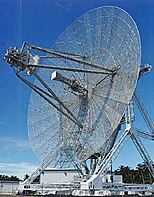
\includegraphics[width=\textwidth]{figures/Radar_antenna.jpg} 
        \caption{Radar antenna} 
        \label{fig:intro-radar} 
    \end{subfigure} 
    \begin{subfigure}[b]{0.48\textwidth} 
        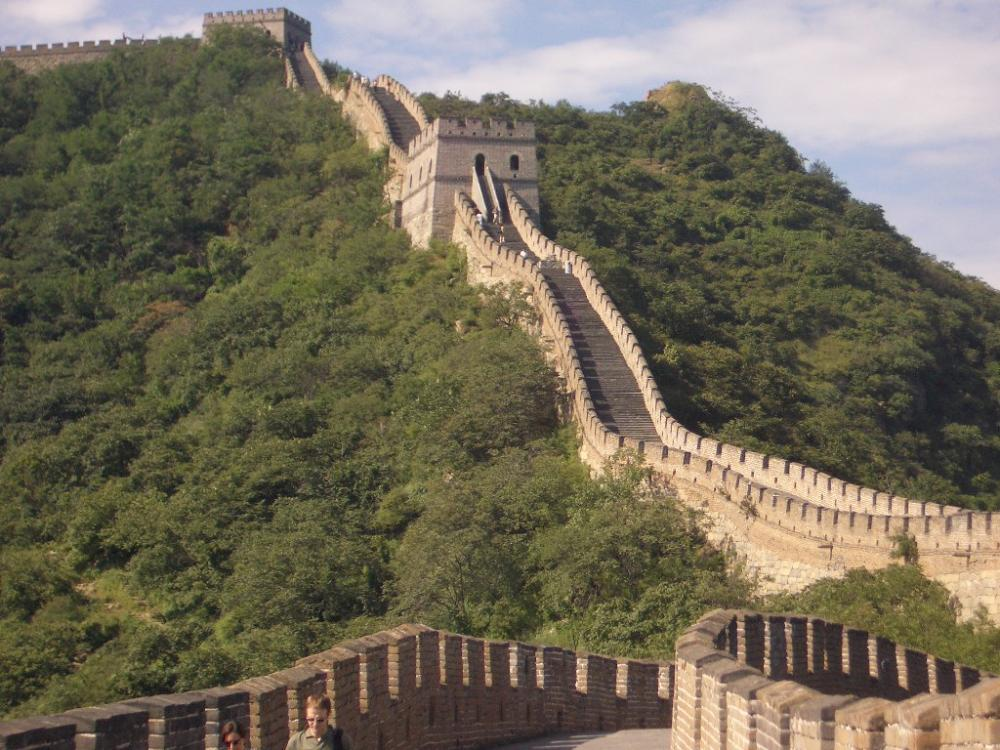
\includegraphics[width=\textwidth]{figures/great_wall.jpg} 
        \caption{Watch towers on the great wall} 
        \label{fig:intro-great_wall} 
    \end{subfigure}
    \caption{Two examples of intrusion detection systems}
    \label{fig:intro-IDS}
\end{figure} 

In surveillance or tracking systems (\ref{fig:intro-laser}), 
sensors like laser beams or cameras are deployed for purposes like thief detection, 
motion capture, pose tracking and so on. 
\begin{figure}[ht] 
    \centering 
    
    % \begin{subfigure}[b]{0.55\textwidth} 
    %     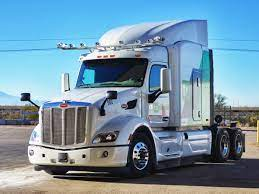
\includegraphics[width=\textwidth]{figures/truck_cam.jpeg} 
    %     \caption{Autonomous truck camera system} 
    %     \label{fig:intro_truckcam} 
    % \end{subfigure} 
    \begin{subfigure}[b]{0.41\textwidth} 
        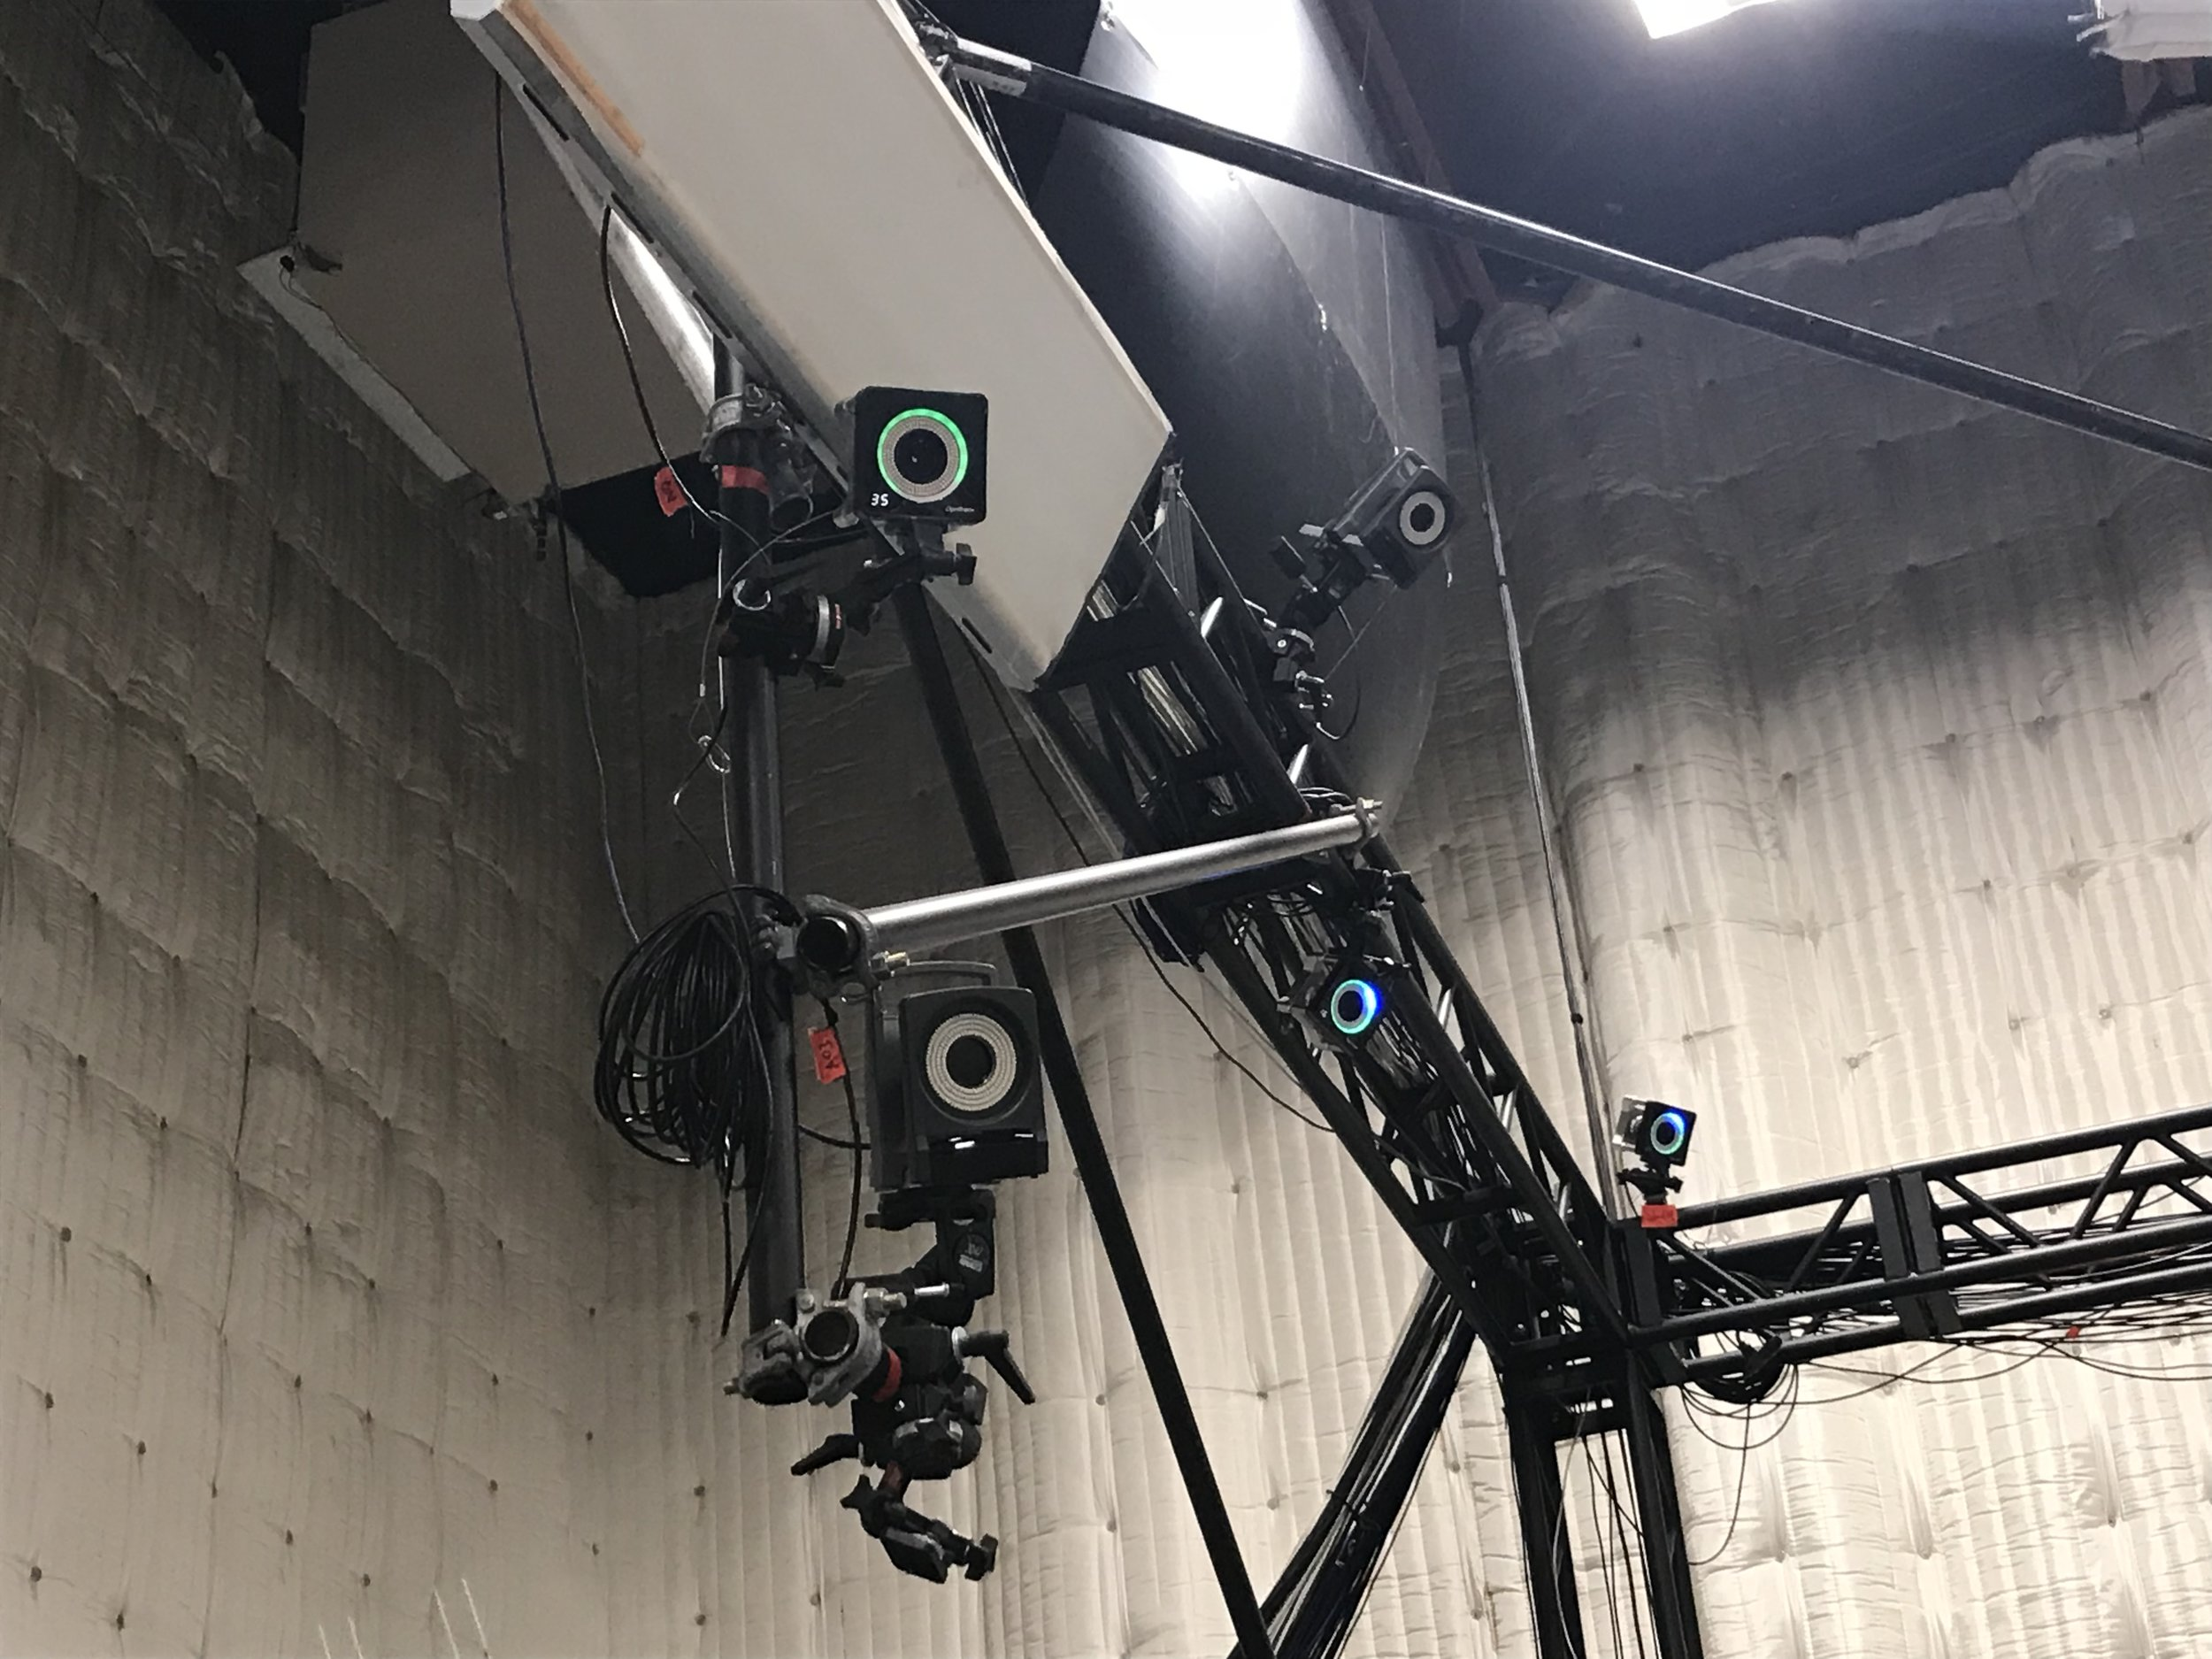
\includegraphics[width=\textwidth]{figures/optitrack.jpg} 
        \caption{Optical tracking system} 
        \label{fig:intro-optitrack} 
    \end{subfigure} 
    \hfill
    \begin{subfigure} [b]{0.46\textwidth} 
        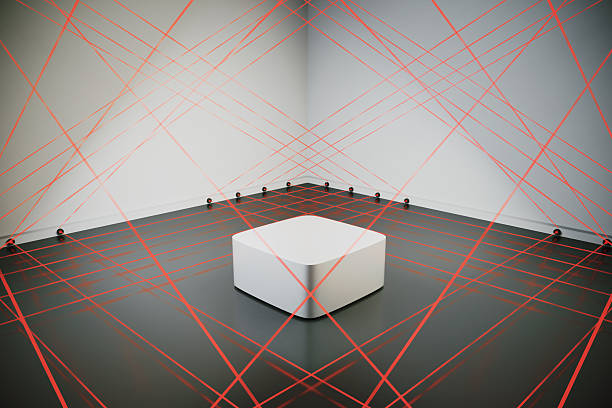
\includegraphics[width=\textwidth]{figures/laser.jpg} 
        \caption{Laser system} 
        \label{fig:intro-laser} 
    \end{subfigure} 
    \caption{Indoor tracking and surveillance systems}
    \label{fig:intro-indoor}
\end{figure}

The deployment of sensors is not limited only to deploying sensors static to the ground.
A notable example is the advent of self-driving cars.
On top of those autonomous vehicles, sensor systems are indispensable for obstacle avoidance and interactions between vehicles.
Tesla (~\ref{fig:intro-tesla}) uses 12 ultrasonic sensors 
near the front and rear bumper, as well as other radars and cameras,
but later changed into a vision system with only cameras 
\footnote{\url{https://www.tesla.com/en_eu/support/transitioning-tesla-vision}}. 
And TuSimple, an autonomous truck company, employs a combination of cameras, radars and lidars 
for their perception system \footnote{\\\url{https://www.tusimple.com/blogs/tusimple-1000-meter-perception-system}}. 
The layout of these sensors on an autonomous vehicle is important for reducing blind spots and casualties caused by them,
% and for budget issues caused by the price of those high-accuracy and long-range sensors.

\begin{figure}[ht] 
    \centering 

    \begin{subfigure}[b]{0.49\textwidth} 
        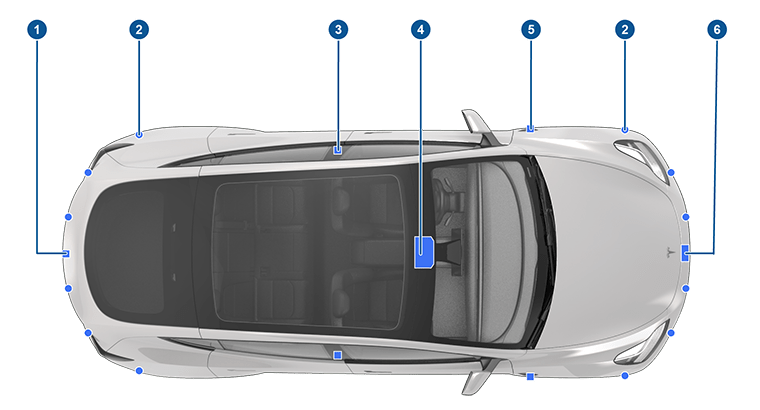
\includegraphics[width=\textwidth]{figures/tesla.png} 
        \caption{
        Tesla Model Y's sensing system
        equipped with cameras (\circled{\small{1}}, 
        \circled{\small{3}}, 
        \circled{\small{4}}, \circled{\small{5}}),
        ultrasonic sensors \circled{\small{2}}, and a radar \circled{6}.
        }
        \label{fig:intro-tesla} 
    \end{subfigure} \hfill
    \begin{subfigure}[b]{0.4\textwidth} 
        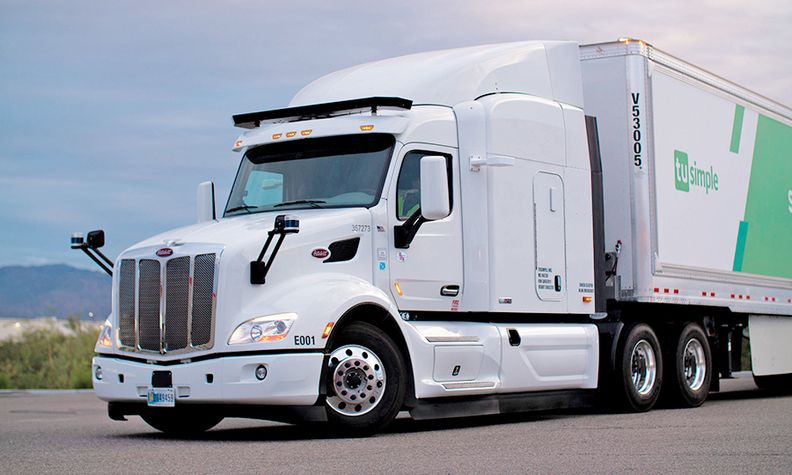
\includegraphics[width=\textwidth]{figures/tusimple.jpg} 
        \caption{TuSimple autonomous truck equipped with CMOS long-range cameras, 
        LiDARs and radars} 
        \label{fig:intro-truckcam} 
    \end{subfigure} 
    \caption{Sensor systems on autonomous vehicles}
    \label{fig:intro-autonomous-vehicles}
\end{figure} 

The placement of sensors is extremely crucial for many reasons.
First, a typical high-frequency tracking camera can cost up to several thousand US dollars in 2023, 
let alone sensors with specific industrial or military purposes. If a certain sensor layout solution
can reduce the number of sensors used in, e.g., in a secure environment, on an autonomous vehicle, or on a patrolling robot,
the cost for deployment of such sensor systems can be greatly reduced.
Second, real sensors come with many characteristics as mentioned in \cite{sebastian2005prob},
range sensors can have noise, unexpected objects blocking the view, sensing failures, random measurements and so on.
Hence, the objective that a sensor system being more balanced in terms of workload is a reasonable assumption
when quality assurance and fault tolerance are the main concerns for the system. 
Lastly, a good sensor deployment in systems like surveillance camera systems means less human labor from the security personnel;
and less energy consumption.
\section{Background}
In this section, we provide sufficient background knowledge and terms used in this dissertation, 
they will be used without explanation in the following chapters. 

\subsection{NP and NP-hardness}
% In the area of optimization, which this thesis is focusing on, NP-hardness has the 
% The definitions are taken from \cite{vazirani2001approximation}
\begin{definition}[Nondeterministic Polynomial (NP)]
    A language $L\in NP$ if there is a polynomial $p$ and a polynomial time-bounded Turing machine M, 
    called the {\textit verifier}, such that for each string $x\in \{0, 1\}^*$: 
    \begin{itemize}
        \item if $x\in L$, then there is a string $y$ (the certificate) of polynomially bounded length, i.e., $|y| \leq p(|x|)$,
        such that $M(x, y)$ accepts, and 
        \item if $x\notin L$, then for any string $y$, such that $|y|\leq p(|x|)$, $M(x,y)$ rejects.
    \end{itemize}
\end{definition}

A colloquial way in \cite{vazirani2001approximation} to describe NP is the class of problems that have ``short and quickly verifiable'' 
Yes certificates.
% NP-complete problems refers to the class of problems such that every problem in NP can be reduced to it.
And an NP-hard problem is a problem that every problem in NP can reduce to it.
Typically, when we call an optimization problem NP-hard, it means the decision version of it is NP-hard.
\subsection{Integer programming}
Since most natural optimization problems are NP-hard, mathematical programming tools are often 
used for solving the problem for its generality and efficiency. Essentially, they take in
some mathematical models including a set of integral variables $x_1, \dots, x_n$ and a set of constraints,
\begin{align*}
    a_{11} x_{11} + \dots + & a_{1n} x_{1n} \geq b_1,\\
    \dots & \\
    a_{m1} x_{m1} + \dots + & a_{mn} x_{mn} \geq b_m,
\end{align*}
and objective 
\[
    \min a_{11} x_{11} + \dots + a_{1n} x_{1n}.
\]
When the variables $x_1, \dots, x_n$ contain continuous variables (continuum), the model becomes a mixed integer programming problem (MILP).

% e.g., its usage in Multi-robot Path Planning Problem (MRPP) \cite{HanYu19IROS, GuoHanYu21ICRA}, sensor coverage. 
Commercial (mixed) integer programming tools include Gurobi \cite{optimization2019gurobi}, IBM CPLEX \cite{cplex2009v12}, and so on,
while open-source libraries include SCIP \cite{achterberg2009scip}, CBC \cite{forrest2005cbc}, GLPK \cite{makhorin2008glpk}, and so on. 
Modern tools, even in the open-source branch, are pretty mature and developed, and hard to optimize within the framework itself. 
While work like \cite{deits2014footstep} in bipedal robot footstep planning and \cite{guo2021spatial} in multi-robot path planning 
seek performance improvement by constructing different instance formulations.

\subsection{Approximation algorithm}
For an optimization problem $\Pi$, OPT($\Pi$), or sometimes OPT, 
denotes the optimal solution of the problem instance. An $(1+\alpha)$-OPT or a $(1+\alpha)$-optimal solution refers
to a solution with an objective value of $(1+\alpha)$OPT for a minimization objective. For the maximization objective,
the corresponding term is $(1-\alpha)$OPT.

Now we give the definition of PTAS and FPTAS.
\begin{definition}[Polynomial Time Approximation Scheme (PTAS)]
    Given any $\varepsilon>0$, if an algorithm $\mathcal A$ runs in polynomial time to the input length. 
    Then if $\mathcal A$ can provide a $(1+\varepsilon)$-OPT solution, the algorithm is called PTAS.
\end{definition}

\begin{definition}[Fully Polynomial Time Approximation Scheme (FPTAS)]
    Given any $\varepsilon>0$, if an algorithm $\mathcal A$ runs in polynomial time to the input length and $1/\varepsilon$. 
    Then if $\mathcal A$ gives a $(1+\varepsilon)$-OPT solution, the algorithm is called FPTAS.
\end{definition}
\section{Problems Studied in the Dissertation}
In this section, we provide an overview of the problems studied in the later chapters, 
where each chapter is independent and self-contained. 

\begin{figure}[h]
    \centering
    \begin{subfigure}[b]{0.4\textwidth}
        \centering
        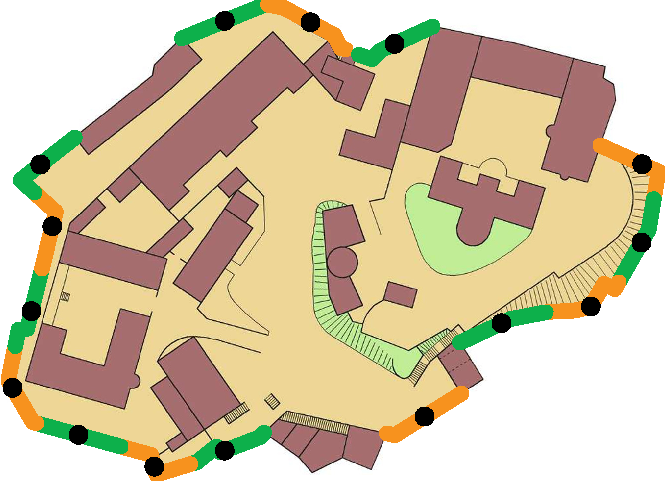
\includegraphics[width = \textwidth]{chapters/opg/figures/castle_15-eps-converted-to.pdf}
        \caption{Optimal perimeter guarding with homogeneous sensors}
        \label{fig:intro-opg-ho}
    \end{subfigure}
    \begin{subfigure}[b]{0.4\textwidth}
        \centering
        \reflectbox{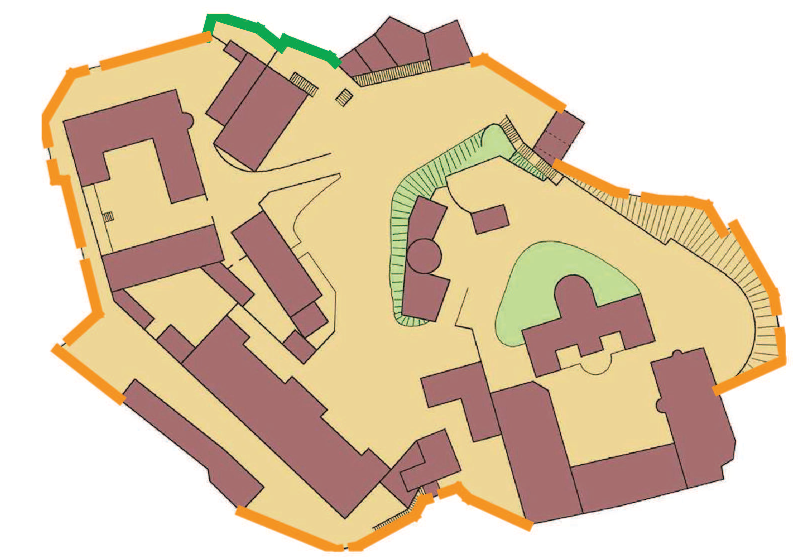
\includegraphics[width = \textwidth, angle=180]{chapters/opg-ext/figures/opgmc-castle-thin-eps-converted-to.pdf}}
        \caption{Optimal perimeter guarding with heterogeneous sensors}
        \label{fig:intro-opg-he}
    \end{subfigure}
    \caption{Optimal perimeter guarding}
    \label{fig:intro-opg}
\end{figure}


The first set of problems we studied relate to optimally assigning a larger number of sensing
robots (or other types of autonomous agents) to guard the perimeters of closed 2D regions,
where the perimeter of each region to be guarded may contain multiple disjoint polygonal chains.
Each robot is responsible for guarding a subset of the perimeter and any perimeter must be guarded
by at some robot.
The sensing range of each robot is assumed to be a continuous line on top of the perimeter of some regions. 
Specifically, two problems will be introduced, perimeter guarding with homogeneous sensors (~\ref{fig:intro-opg-ho}),
and with heterogeneous sensors (~\ref{fig:intro-opg-he}). 
The homogeneous case can be solved using only classical algorithms. 
While the heterogeneous case is NP-hard, but can still be solved with dynamic programming under a reasonable
amount of time. 


\begin{figure}[h]
    \centering
    \begin{subfigure}[b]{0.4\textwidth}
        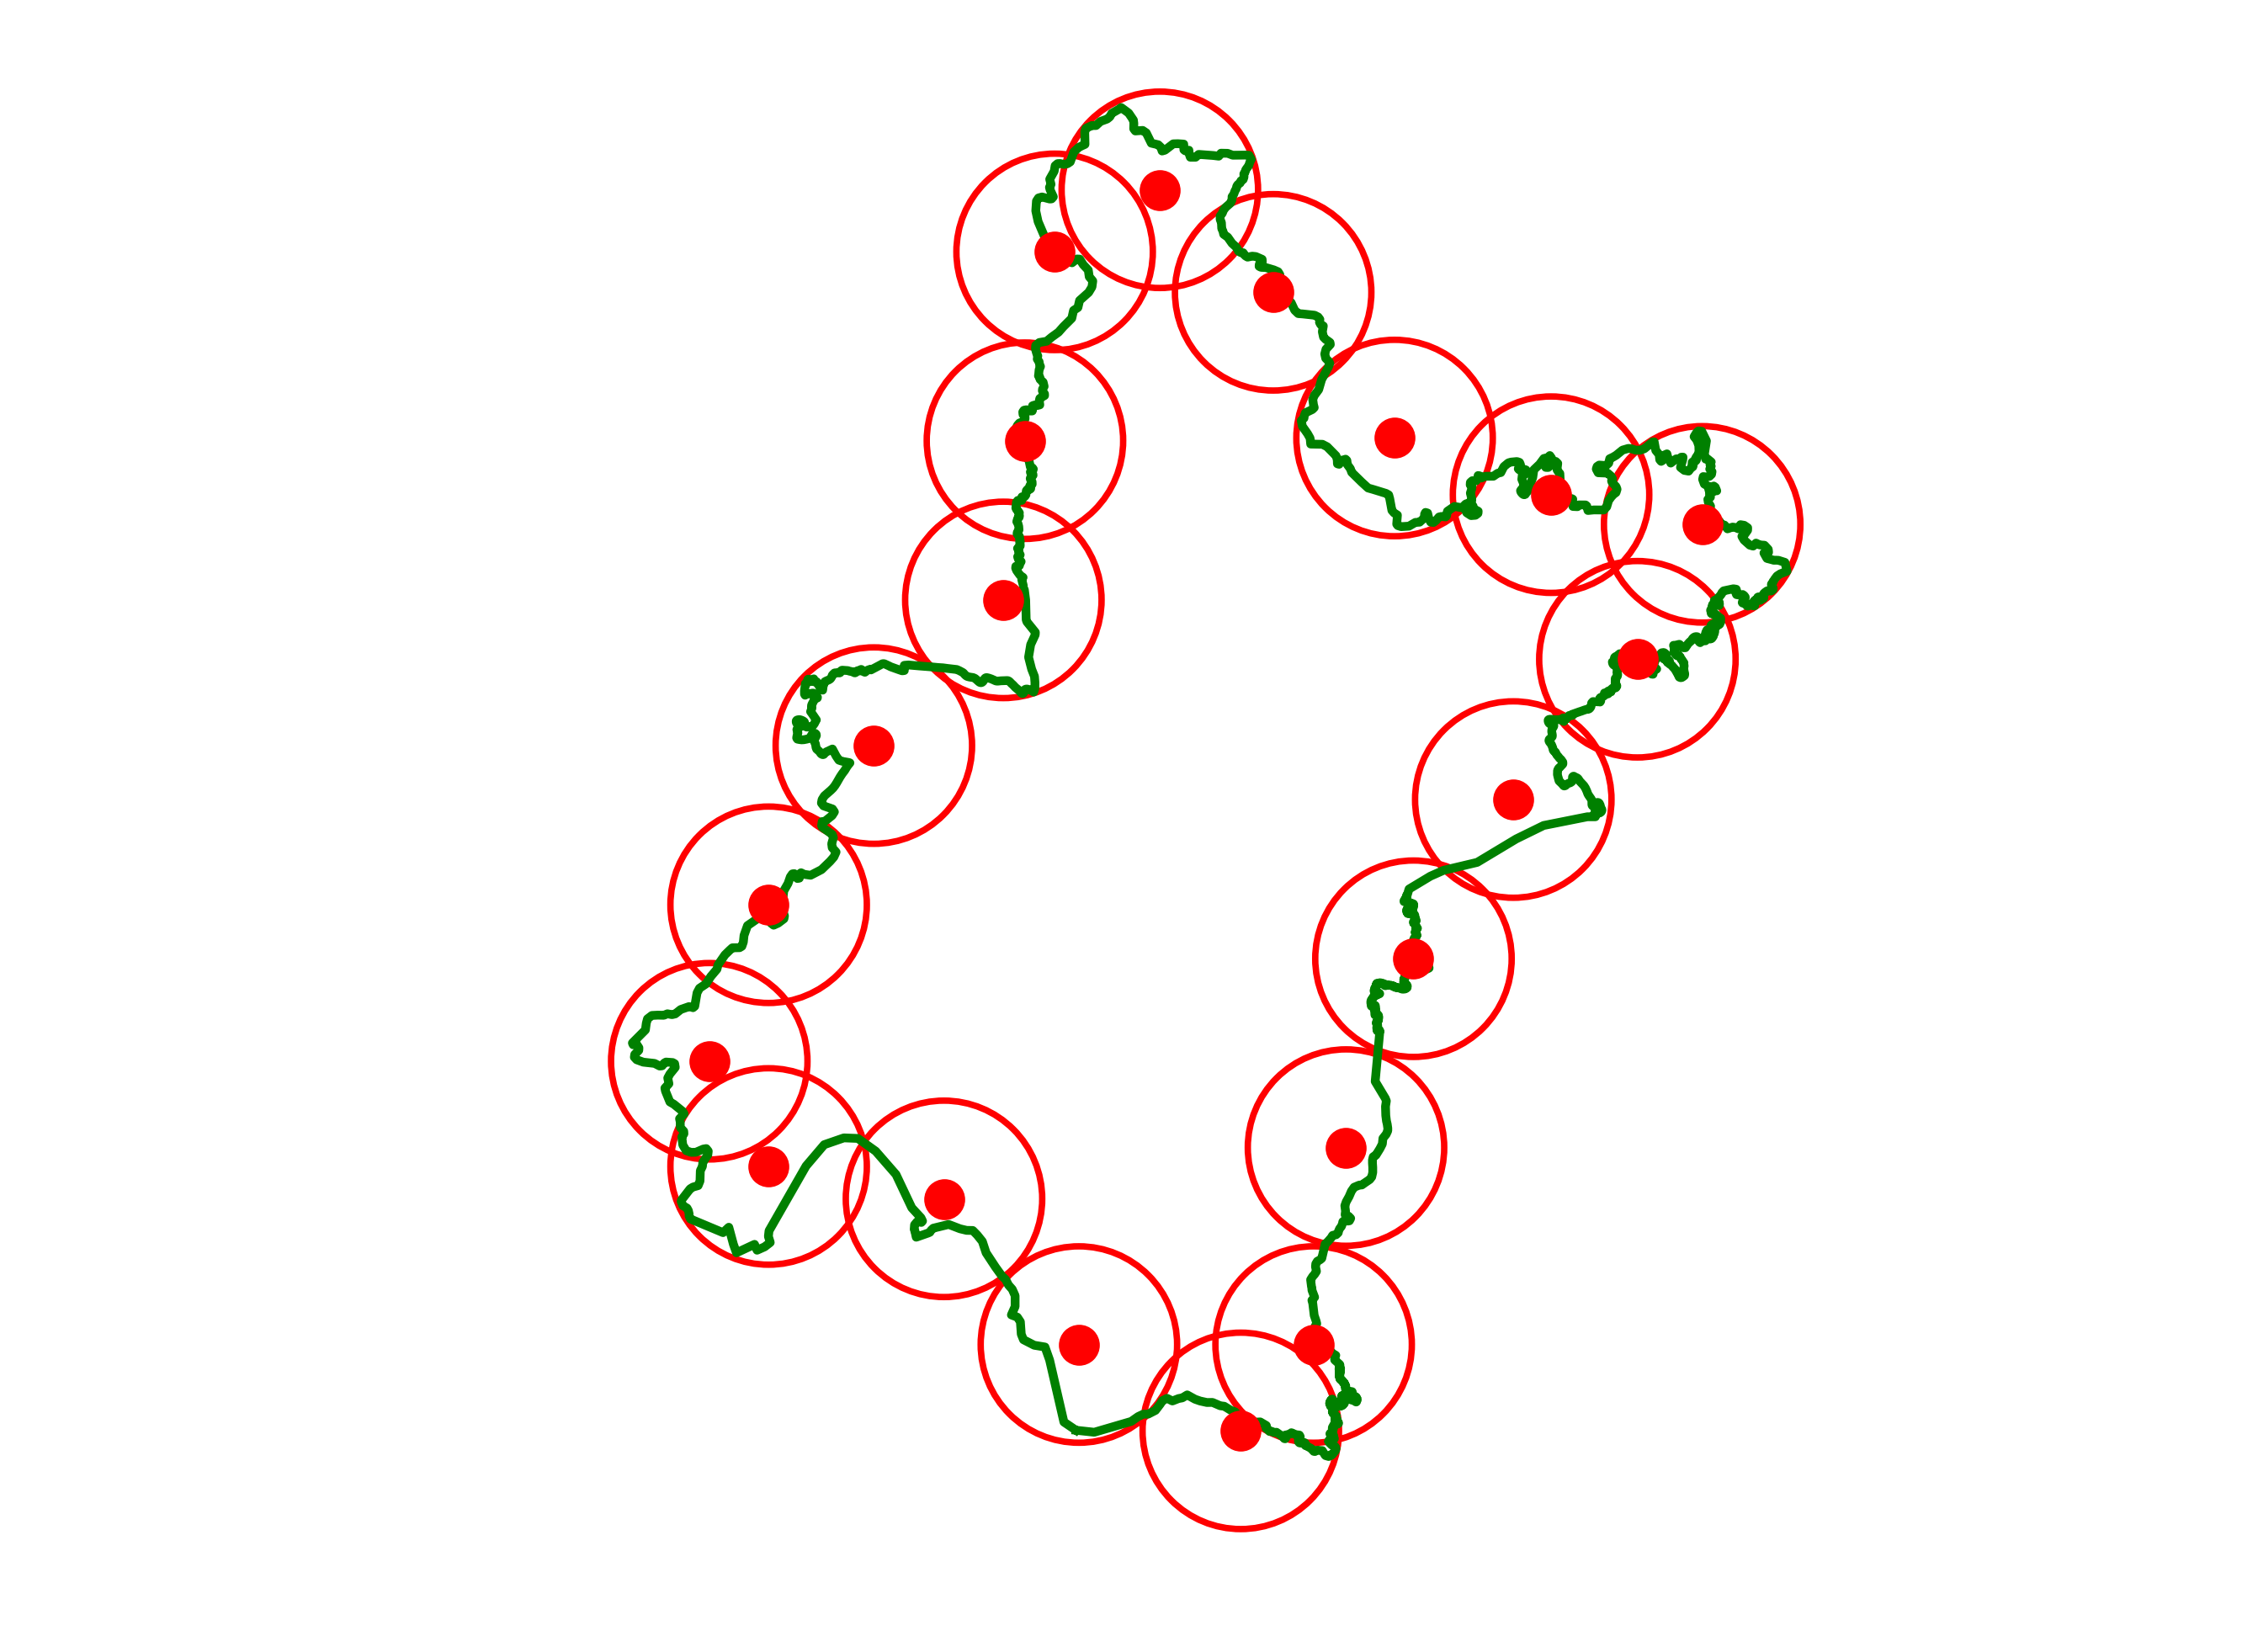
\includegraphics[width = 1.2\textwidth]{chapters/osg/figures/wuhan_ilp.png}
        \caption{Optimal perimeter guarding with 2D range sensors}
        \label{fig:intro-opg2d}
    \end{subfigure}
    \begin{subfigure}[b]{0.4\textwidth}
        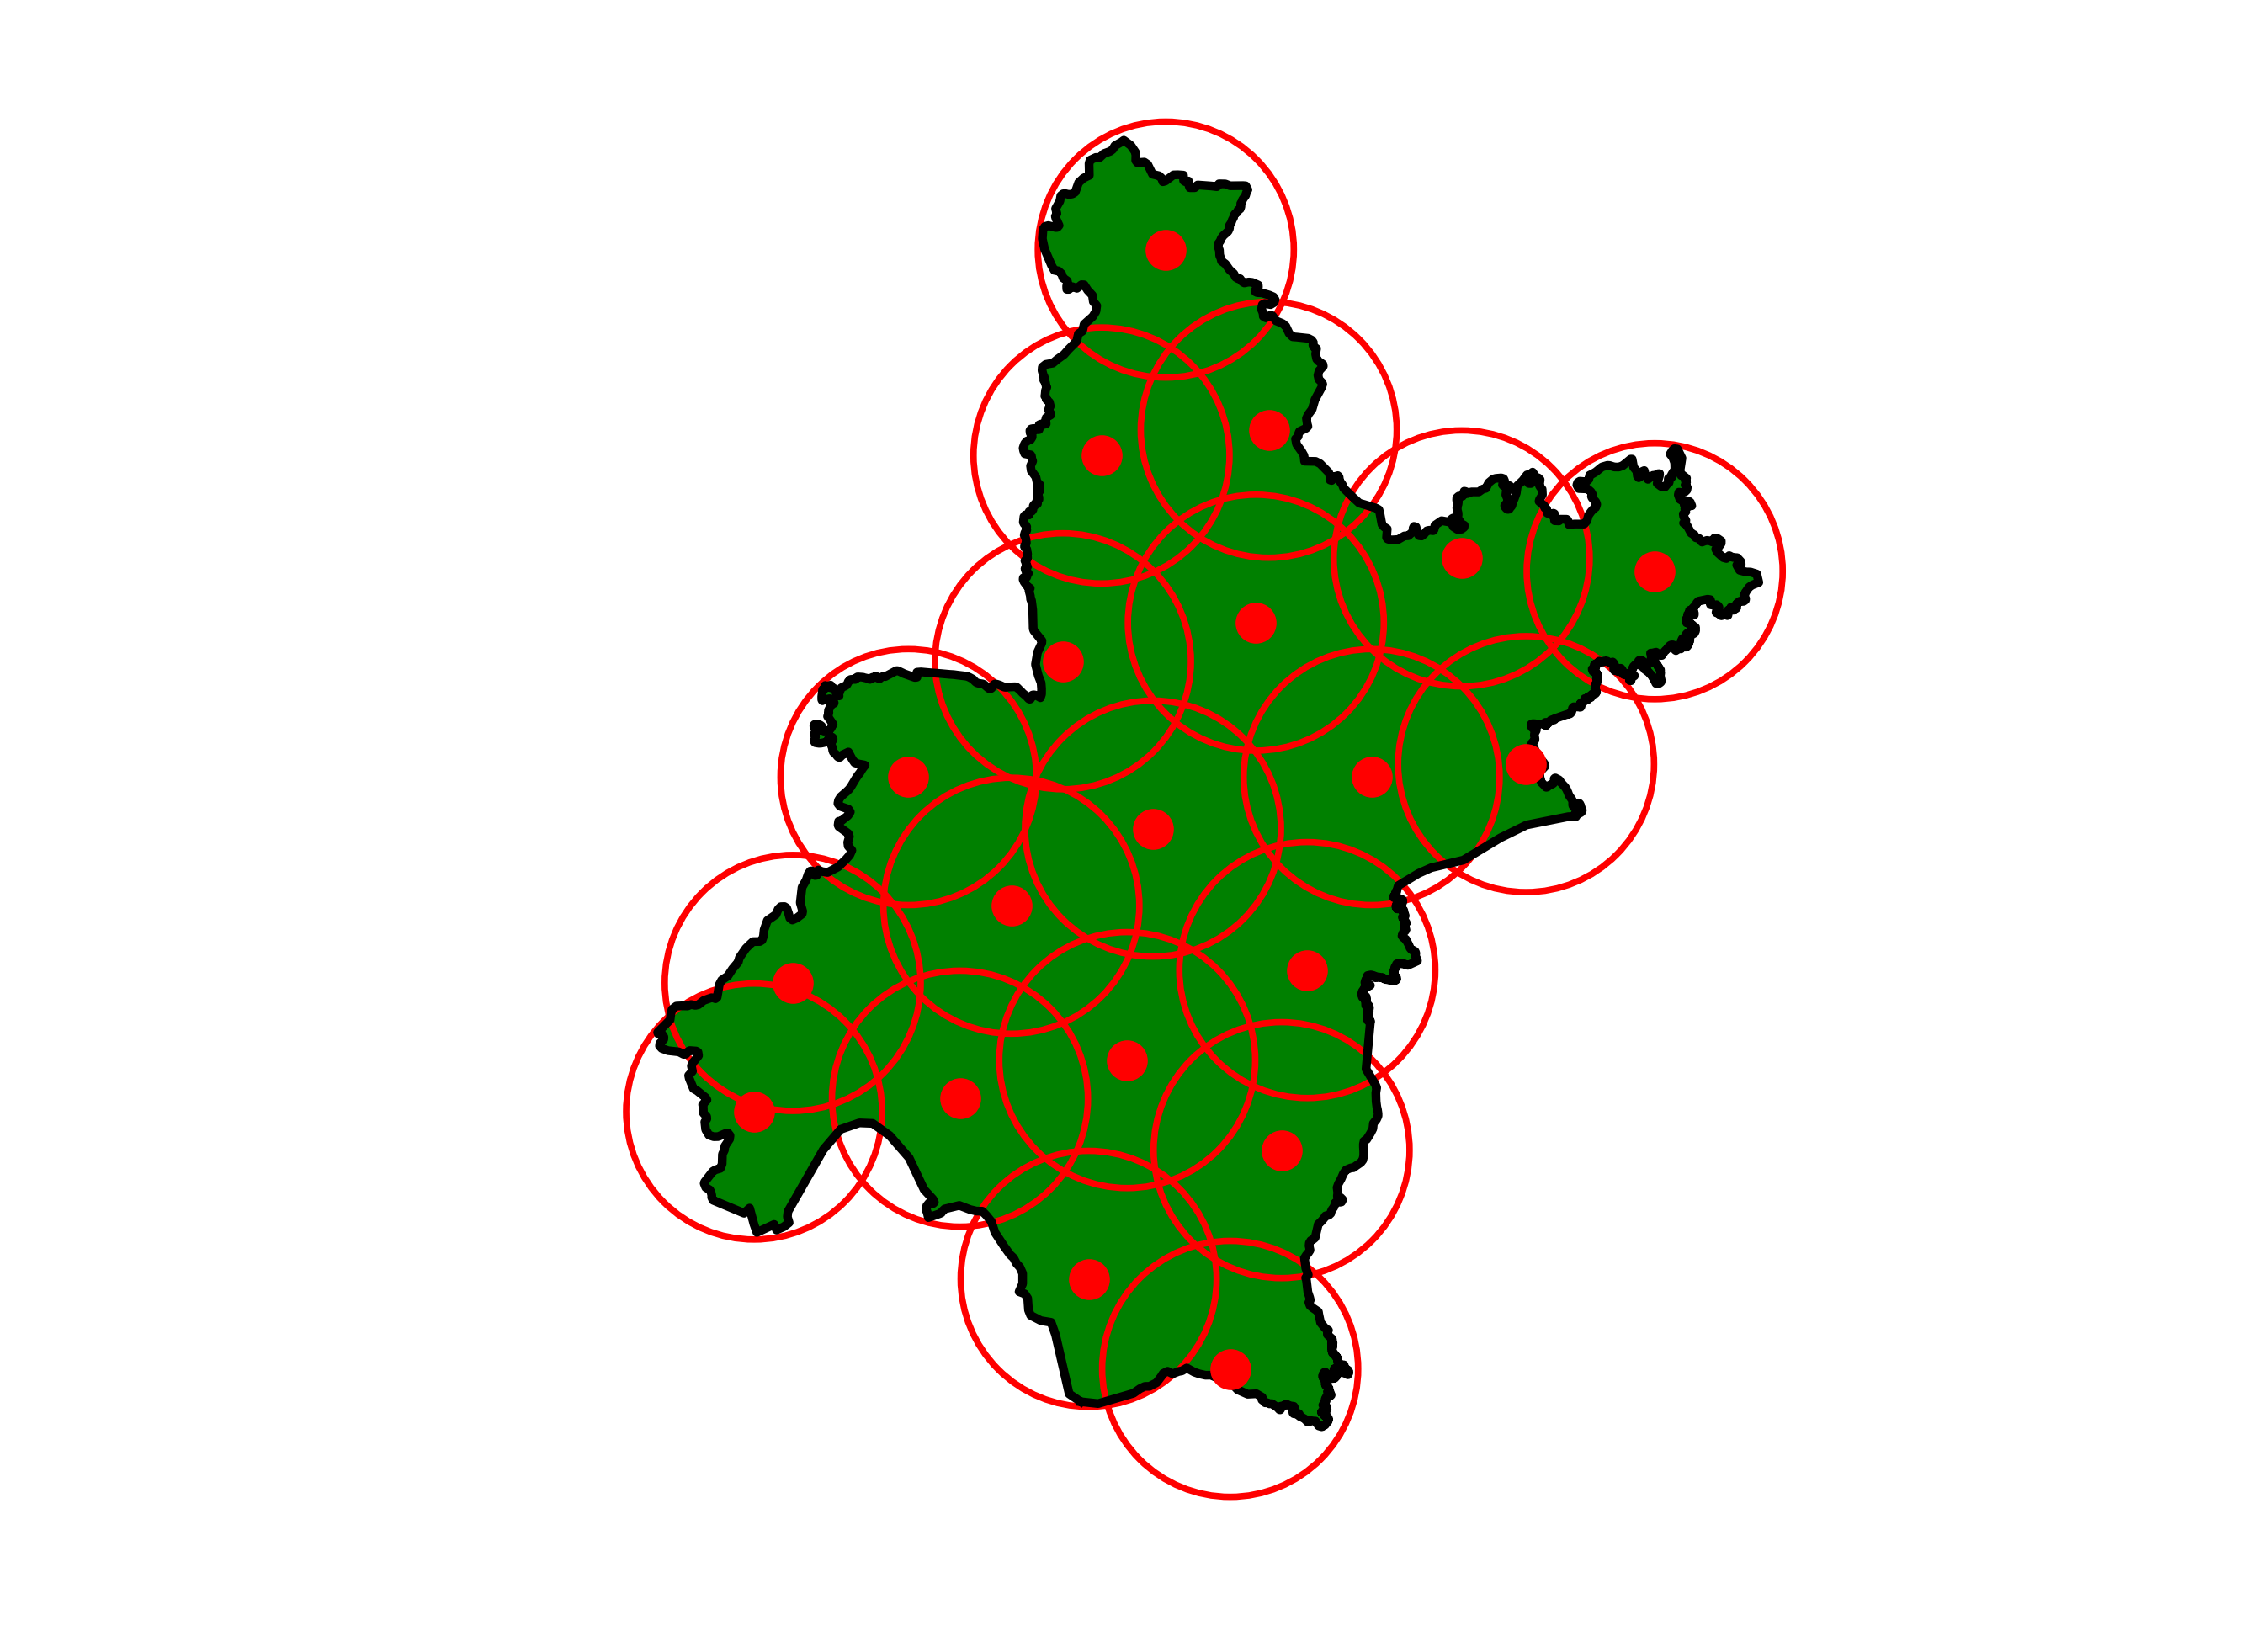
\includegraphics[width = 1.2\textwidth]{chapters/osg/figures/wuhan_region_ilp.png}
        \caption{Optimal region guarding with 2D range sensors}
        \label{fig:intro-org2d}
    \end{subfigure}
    \qquad
    \qquad
    \caption{Optimal set guarding with 20 sensors to cover the perimeter and interior of a city}
    \label{fig:intro-osg}
\end{figure}
Then, we continue with perimeter guarding but use 2D circles to represent the 
coverage range of sensors. The study extends to guarding 2D regions beyond the perimeters. 
When given a bounded $\mathbb R^2$ to be guarded, and $k$ mobile sensors with variable sensing ranges of $r_1,\dots,r_k$, 
our objective is to minimize $\max_{i=1}^{k} r_i$.
Our study shows that even for covering the boundary or interior of a simple polygon, 
the problem of finding the minimum sensing radius is NP-hard to approximate within a factor of 1.152, i.e.,
unless P=NP, there is no polynomial solution for finding a $1.152$ optimal solution. 
However, on the side of computational methods, we develop a fully polynomial time approximation algorithm for covering
a perimeter with a reasonable assumption of continuous coverage.


\begin{figure}[h]
    \centering
    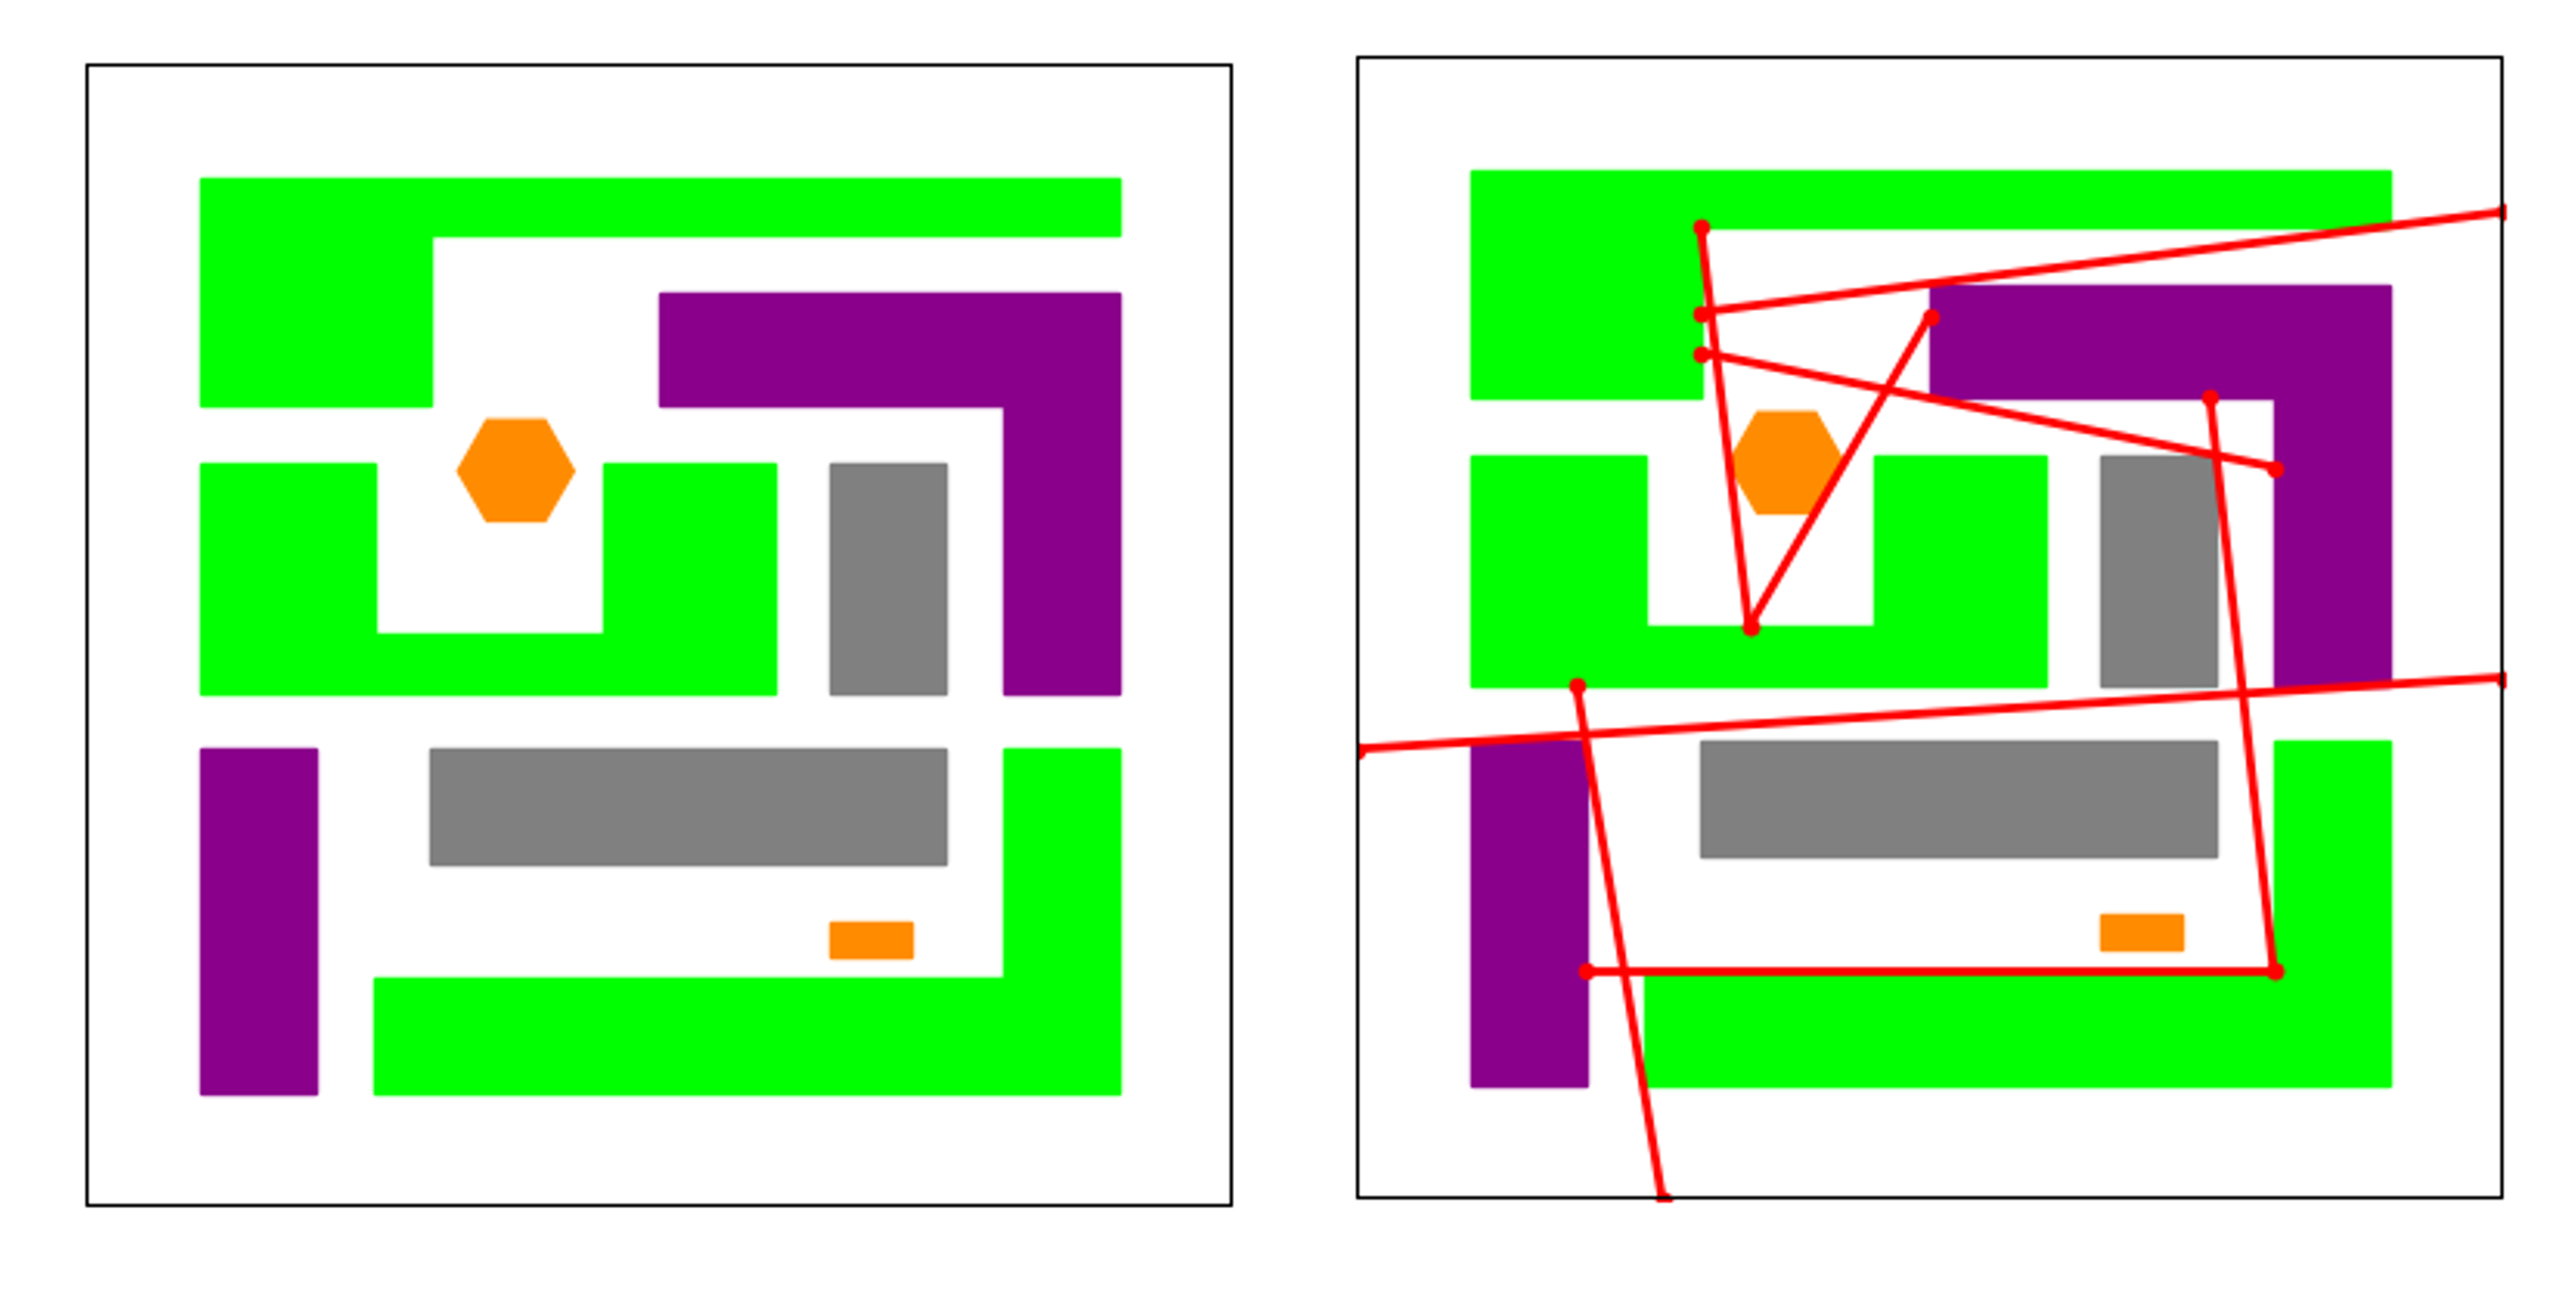
\includegraphics[width = 0.5\textwidth]{chapters/bf/fig/intro_pic.png}
    \caption[Separating three sets of building blocks with the existence of two obstacles]{Separating three sets of building blocks (orange, purple and green) with the existence of two grey obstacles.}
    \label{fig:intro-lines}
\end{figure}


After two chapters' discussion on covering perimeters or regions, which is essentially separating 
some critical polygonal regions from the outside workspace. 
The fourth chapter digs deeper into this problem by studying the separation of more than two regions. 
To simplify the problem, a line-of-sight sensing model will be adopted, where each sensor can cover
an unobstructed line segment like a laser beam. Also, the regions are assumed to be polygonal.
The objective in this case is to minimize the number of sensors used to separate these polygonal sets 
at the existence of obstacles (see ~\ref{fig:intro-lines}).
This problem is termed as the barrier forming problem \cite{feng2022barrier}.
The problem is NP-hard even for the problem of separating two sets of regions with the minimum number of lines. 
Still, integer programming can provide a near-optimal solution for around 20 objects in a reasonable amount of time. 

\begin{figure}[h]
    \centering
    \vspace{-.8in}
    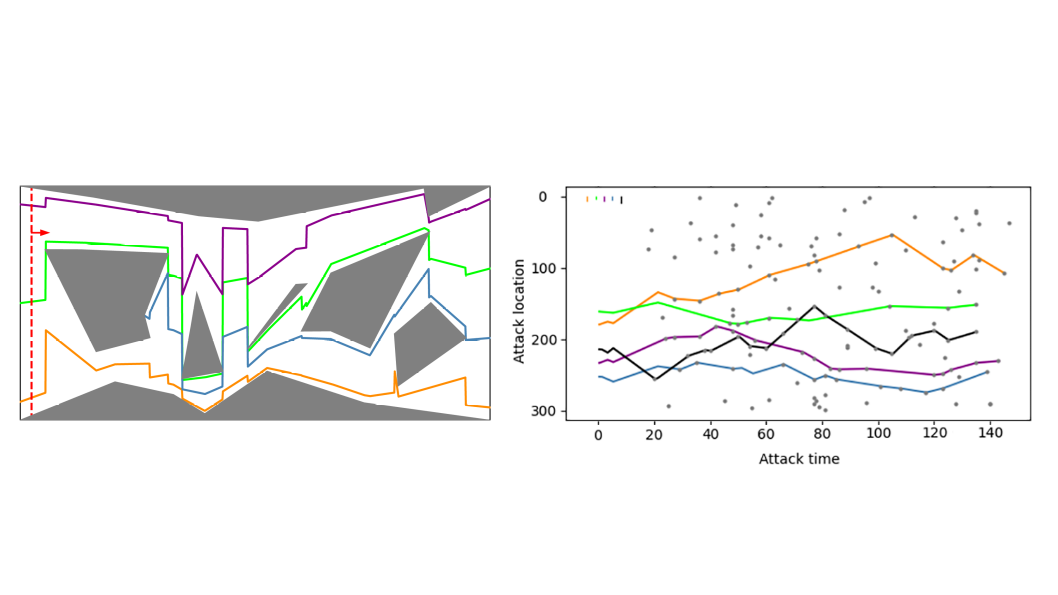
\includegraphics[width=.8\textwidth]{figures/dynamic-intro.png}
    \vspace{-.5in}
    % {
    %     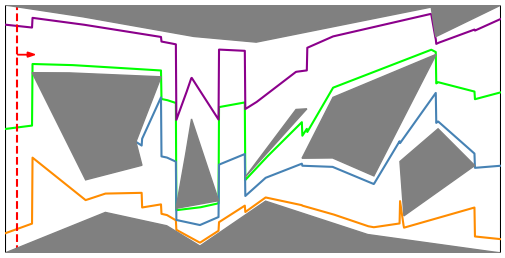
\includegraphics[width = 0.35\textwidth]{chapters/sc/fig/instance_2.png}
    % }
    % 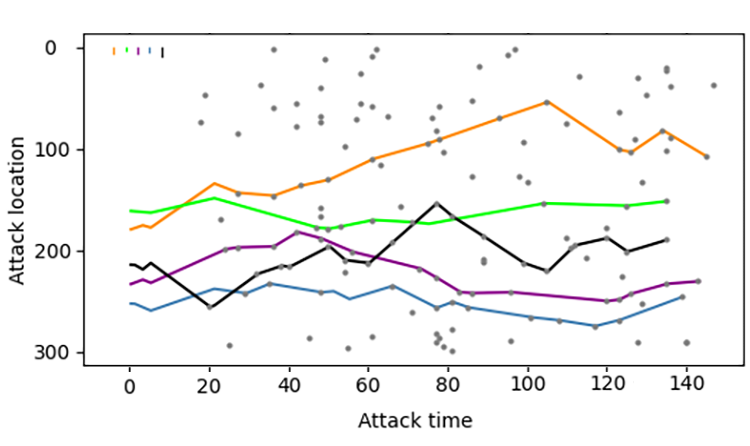
\includegraphics[width = 0.35\textwidth]{chapters/bd/fig/inf_horizon_example-v.png}
    \caption[Illustration of sweeping and boundary defense]{[left] the coordinated sweeping problem, [right] the perimeter defense problem.}
    \label{fig:intro-bd-sc}
\end{figure}

The fifth chapter deals with the dynamic setting for mobile sensing robots, 
and two different but related problems are studied. 
The first problem is the boundary defense problem in the context of heterogeneous defenders, which was first studied in \cite{adler2022role}.
It can be seen as an extension of the perimeter defense problem \cite{shishika2020review}. 
In this problem, there are $k$ sensing robots moving on top of a perimeter with different speeds $v_1,\dots,v_k$.
A sequence of attacks $\langle loc_i, t_i \rangle_{i=1}^{n}$ are given at different time stamps and at different locations.
The objective is to intercept as many attacks as possible.
The second problem is the coordinated sweeping problem \cite{feng2023optimal} where a group of robots coordinate to sweep a region 
with obstacles. Each robot possesses a given sensing capability, and the sweeping trajectory is 
given beforehand. The objective of it is to minimize the number of robots used such that the sweeping plan 
can be executed and every point in the workspace is sensed with a certain required quality. 

\begin{figure}[ht]
    \centering
    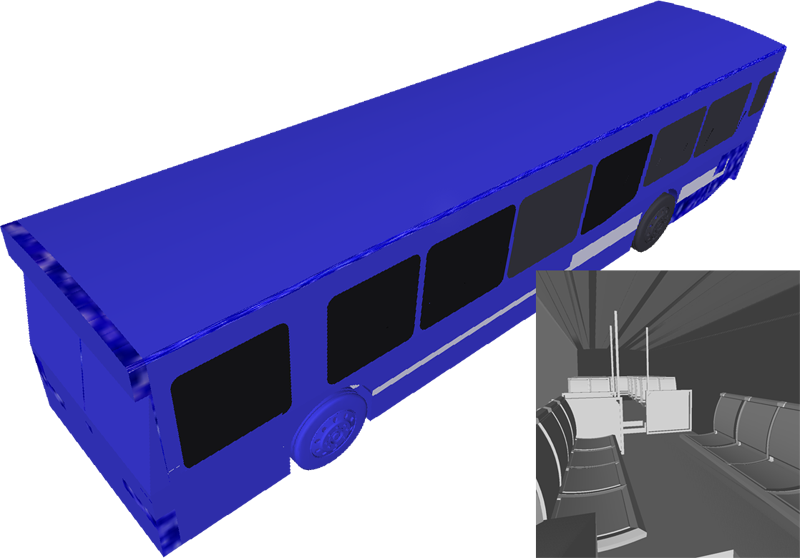
\includegraphics[width = 0.45\textwidth]{chapters/surf/fig/bus.png}
    \hfill
    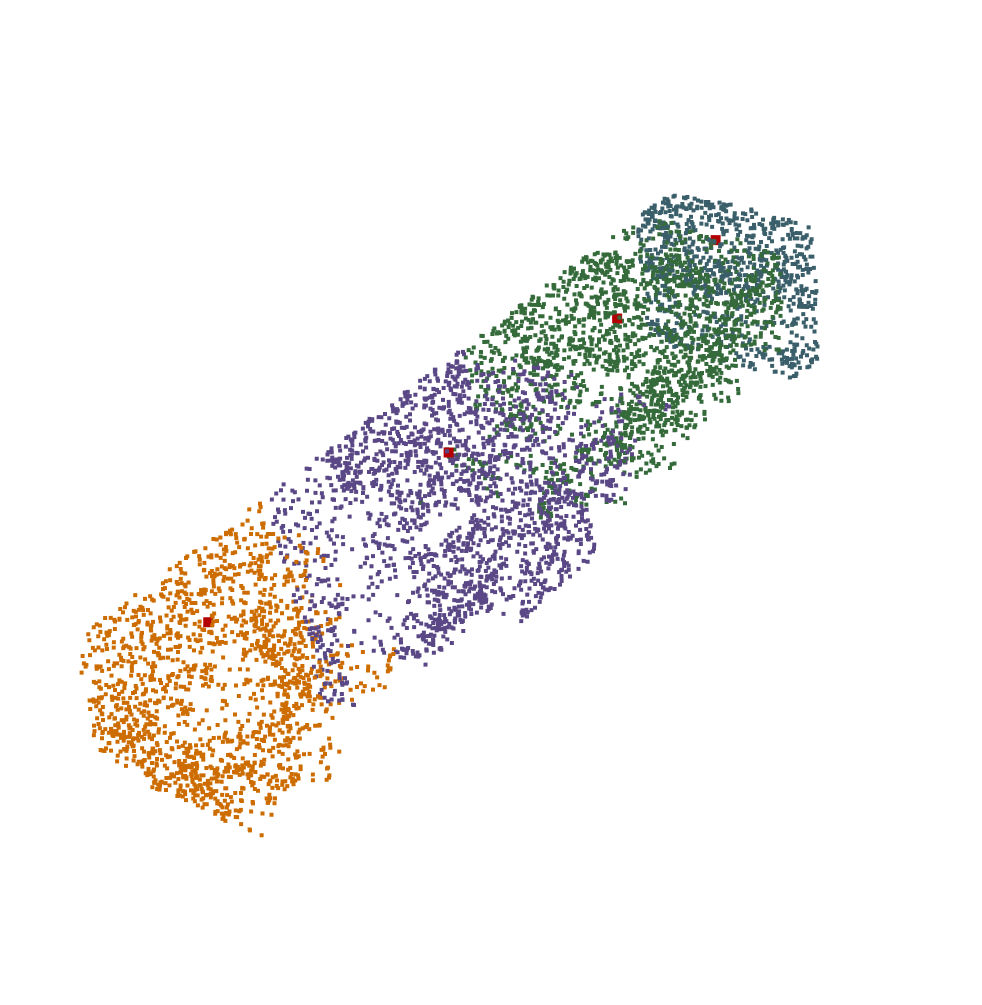
\includegraphics[width = 0.4\textwidth]{chapters/surf/fig/bus_result_3.png}
    \caption{UV sanitization lights placement to cover the interior of a bus}
    \label{fig:intro-surf}
\end{figure}

The sixth chapter discusses a real-world application in the placement of UV (ultraviolet) lights 
to cover the surface of an environment for sanitization purposes \cite{feng2021sensor}. The problem can be seen as an extension
of the art-gallery problem \cite{o1987art}, and thus computationally intractable.
Still, a combined integer programming and classical local search approach can be used to
solve the problem effectively. The method is evaluated on three real scenarios: 
the interior of a bus, a subway or an ICU room. 


\section{Literature review} 

% On the other hand, 

\subsection{Coverage-related problems in computational geometry}

For tackling multi-sensor coverage, problems studied in this thesis are intimately connected to the Art 
Gallery problems \cite{o1987art,shermer1992recent}, with origins traceable 
to half a century ago \cite{klee1969every}. Art Gallery problems assume 
a visibility-based \cite{lozano1979algorithm} sensing model; in a typical 
setup \cite{o1987art}, the {\em interior} of a polygon must be visible to at 
least one of the guards, which may be placed on the boundaries, corners, 
or the interior of the polygon. Finding the optimal number of guards are 
often NP-hard \cite{lee1986computational}. Alternatively, a disc-based sensing 
model may be used, which leads to the classical {\em packing} problem 
\cite{thue1910dichteste,hales2005proof}, where no overlap is allowed between 
the sensors' coverage area, the {\em coverage} problem 
\cite{drezner1995facility,cortes2004coverage,pavone2009equitable,martinez2010distributed,pierson2017adapting}, 
where all 
workspace must be covered with overlaps allowed, or the {\em tiling} problem 
\cite{kershner1968paving}, where the goal is to have the union of sensing
ranges span the entire workspace without overlap. For a more complete 
account on Art Gallery, packing, and covering, see Chapters 2, 3, and 33 of
\cite{toth2017handbook}. Despite the existence of a large body of literature 
performing extensive studies on these intriguing computational geometry 
problems, these types of research mostly address domains that are 2D and 
higher.



% Recently, the problems of globally optimally covering perimeters using 
% one-dimensional sensors have been studied in much detail 
% \cite{fenghangaoyu2019efficient,fengyu2020RAL}. It is shown that when the sensors 
% are homogeneous, the optimal deployment of sensors can be computed 
% very efficiently, even for highly complex perimeters \cite{fenghangaoyu2019efficient}.
% On the other hand, the problem becomes immediately intractable, sometimes
% strongly NP-hard, when sensors are heterogeneous \cite{fengyu2020RAL}. 
% Our research is distinct from \cite{fenghangaoyu2019efficient,fengyu2020RAL} in that 
% we employ a (two-dimensional) range sensing model and work on the coverage 
% of both perimeters and regions, which has much broader applicability. 

As pointed out in \cite{cortes2004coverage,schwager2009decentralized}, 
distributed sensor coverage has roots in the study 
of the facility location optimization problem 
\cite{weber1929theory,drezner1995facility}, which examines the selection 
of facility (e.g., warehouses) locations that minimize the cost of delivery 
of supplies to spatially distributed customers. In theoretical computer 
science and operations research, these are known as the $k$-center, 
$k$-means, and $k$-median clustering problems \cite{har2011geometric}, 
the differences among which are induced by the cost structure. Our 
investigations benefit from the vast literature on 
the study of $k$-center clustering and related problems, e.g., 
\cite{feder1988optimal,hochbaum1985best,gonzalez1985clustering,daskin2000new,shamos1975closest}.
%
These clustering problems are in turn related to packing 
\cite{hales2005proof}, tiling \cite{thue1910dichteste}, and the 
well-studied art gallery problems \cite{o1987art,shermer1992recent}.

% \subsection{Mobile sensing robot coverage control} 
\subsection{Sensor Networks}
Problems studied in this work can be seen as variants or generalizations of the barrier coverage problem in the area of sensor networks.
The concept of barrier coverage originates from \cite{gage1992command}, together with the blanket and sweep coverage. 
In a seminal work \cite{kumar2005barrier}, the $k$-barrier problem was formulated and various probabilistic models were studied. 
In \cite{kloder2007barrier}, the authors solved the min-distance barrier coverage problem optimally under a non-trivial environment to minimize the total length of the barriers between two groups of polygonal objects. 
To tackle the proposed problem, a novel and efficient network-flow-based method is applied. 
Multiple groups of objects are tackled in \cite{abrahamsen2020geometric}.
The following work \cite{kloder2008thesis} includes a similar problem formation to the problem studied in ~\ref{ch:bf}, where the objective is minimizing the number of fixed-length line segments used. 

\subsection{Multi-robot coordination} 
Our work draws inspiration from a long line of multi-robot coverage planning and 
control research, e.g., \cite{cortes2004coverage,martinez2007motion,
schwager2009optimal,pavone2009equitable,schwager2009decentralized,
pierson2017adapting}. 
%
In an influential body of work on coverage control \cite{cortes2004coverage,
martinez2007motion}, a gradient-based iterative method is shown to drive 
one or multiple mobile sensors to a locally optimal configuration with 
convergence guarantees. 
%
Whereas \cite{cortes2004coverage,martinez2007motion} assume that the 
distribution of sensory information is available {\em a priori}, it is 
shown that such information can be effectively learned 
\cite{schwager2009decentralized}. 
%
Subsequently, the control method is further extended to allow the 
coverage of non-convex and disjoint 2D domains \cite{schwager2009optimal} 
and to work for mobile robots with varying sensing or actuation capabilities
\cite{pierson2017adapting}. 
%
In contrast to these control-based approaches, which produce iterative 
locally optimal solutions, our work emphasizes the direct computation of 
globally optimal deployment solutions and supports arbitrarily shaped
bounded (1D) perimeters and (2D) regions.

With an emphasis on robotic swarm deployment, within multi-robot 
systems research \cite{arai2002advances,gerkey2004formal,ren2008distributed,bullo2009distributed}, 
our study is closely related to {\em formation control}, e.g., 
\cite{ando1999distributed,jadbabaie2003coordination,olfati2004consensus,ren2005consensus,cheng2008almost,mesbahi2010graph,yu2012rendezvous},
where the goal is to achieve certain {\em distributions} through 
continuous (often, local sensing-based) interactions among the 
agents or robots. Depending on the particular setting, the 
distribution in question may be spatial, e.g., rendezvous
\cite{ando1999distributed,yu2012rendezvous}, or maybe an agreement 
in agent velocity is sought \cite{jadbabaie2003coordination,ren2005consensus}. 
In these studies, the resulting formations often have some 
degree-of-freedoms left unspecified. For example, rendezvous 
results \cite{ando1999distributed,yu2012rendezvous} often come 
with exponential convergence guarantee, but the location of
rendezvous is generally unknown {\em a priori}. 

In multi-robot task and motion planning problems (e.g.,
\cite{smith2009monotonic,ayanian2010decentralized,liu2011multi,liu2013optimal,turpin2014goal,turpin2014capt,alonso2015multi,SolYu15}), 
especially ones with a {\em task allocation} element 
\cite{smith2009monotonic,liu2011multi,liu2013optimal,turpin2014goal,turpin2014capt,SolYu15},
the (permutation-invariant) target configuration is often mostly 
known. The goal here is to find a one-to-one mapping between individual 
robots and the target locations (e.g., deciding a {\em matching}) and 
then plan (possibly collision-free) trajectories for the robots to reach 
their respective assigned targets \cite{turpin2014goal,turpin2014capt,SolYu15}.  

\subsection{Search and rescue}
The study of the dynamic coverage in this dissertation draws inspiration from the study of several 
lines of related problems. 
The Graph-Clear problem, formulated in \cite{kolling2007graph}, tasks a group of robots to search and clear an environment with the operations of blocking and clearing.
A follow-up work on Line-Clear \cite{kolling2017coordinated} uses line guards
with more focus on computational geometry in that
the objective is to minimize the maximum sweep line distance. Both of these problems are
NP-hard, establishing the difficulties of finding a sweeping schedule for a planar environment.
The more general pursuit-evasion problem dates back to the research on \emph{search number}
on a discrete graph \cite{megiddo1988complexity}, 
followed by studies on pursuit and evasion in continuous environments with 
visibility-based model \cite{guibas1999visibility, suzuki1992searching, lavalle2000algorithm, stiffler2017persistent}. 

When working with known patrolling search frontiers, e.g., vertical sweep lines, 
this sweep line coverage problem is analogous to the perimeter defense problem by placing guards on a static perimeter
to defend intruders \cite{shishika2020cooperative, macharet2020adaptive, chen2021optimal}.
Previously, we have also studied a version of static range guard placement problems for securing perimeters and regions \cite{fengyu2020optimally}.
In contrast to the pursuit-evasion algorithms that deal with searching dynamic and unpredictable targets that could escape, 
coverage planning/control-related algorithms become more suitable for searching or covering predictable or stationary targets,
e.g., room sweeping, pesticide and fertilizer spraying, persistent monitoring, and so on 
\cite{cortes2004coverage, Correia2021icra, oksanen2009coverage, haksar2020spatial, wei2018coverage, deng2019constrained, 
lan2013planning, cassandras2012optimal, yu2015persistent, palacios2017optimal}. 

% The problem becomes the well-known art-gallery problem \cite{o1987art} when a static deployment of robots is sought after.
% In contrast to formation control and multi-robot motion planning research, 
% our study of \opg seeks to determine an exact, optimal distribution 
% pattern of robots (in this case, over a fairly arbitrary, bounded 1D 
% topological domain). Thus, solutions to \opg may serve as the target 
% distributions for multi-robot task and motion planning, which is a main 
% motivation behind our work. The generated distribution pattern is 
% also potentially useful in multi-robot persistent monitoring 
% \cite{soltero2014decentralized} and coverage \cite{howard2002mobile,schwager2009optimal} 
% applications, where robots are asked to carry out sensing tasks in some 
% optimal manner. 
% \subsection{Sensor network} 

% \section{Application}

    
\chapter{Perimeter Guarding}
\thispagestyle{myheadings}

\section{Perimeter Guarding with Homogeneous Defenders}

\subsection{Introduction}


\def\R{\mathcal R}
\def\C{\mathcal C}
\def\S{\mathcal S}
\def\P{\mathcal P}
\def\G{\mathcal G}
\def\W{\mathcal W}
%\thickmuskip=0mu
\def\opg{{\sc {OPG}}\xspace}

Consider the scenario from ~\ref{fig:opg-example}, which contains a closed region with its boundary (or border) demarcated by the red and dotted blue lines. To secure the region, either from intrusions from the outside or unwanted escapes from within, it is desirable to deploy a number of autonomous agents to monitor or guard either the entire boundary or selected portions of it (e.g., the red line segments), with each agent responsible for a continuous section. 
%
Naturally, one might also want to have even coverage by the agents, e.g., minimizing the maximum effort from any agent. In practice, such efforts may correspond to sensing ranges or motion capabilities of robots, which are always limited. 
%
As an intuitive example, the figure may represent the top view of a castle, with its entire boundary being a high wall that may be traversed by agents. 
%
The portion of the wall marked with the three red line segments must be protected, whereas the art marked by the dotted blue lines may not need active monitoring (e.g., the outside may be a cliff or a body of deep water). The green and orange lines show an optimal distribution of the workload by $8$ agents that cover all red segments but skip two of the three-dotted line segments. 

More formally, in this paper, we study the problem of deploying a large 
number of robots to guard a set of one-dimensional boundary segments 
called perimeters. Each perimeter is comprised of one or more 1D segments 
that are part of a circular boundary (e.g., the red segments in 
~\ref{fig:opg-example}). Each robot is tasked to guard a continuous 1D 
segment that covers a portion of a perimeter. As the main objective, 
we seek an allocation of robots such that {\em (i)} the union of the 
robots' coverage encloses all perimeters and {\em (ii)} the 
maximum coverage of any robot is minimized. We call this 1D deployment
problem the Optimal Perimeter Guarding (\opg) problem. 
\begin{figure}[ht]
\vspace*{0mm}
\begin{center}
\begin{overpic}[width=0.7\textwidth,tics=5]{./chapters/opg/figures/example.eps}
%\put(26,20){{\small $R_1$}}
%\put(20,39){{\small \textcolor{red}{$P_1$}}}
%\put(66,28){{\small $R_2$}}
%\put(54,40){{\small \textcolor{green}{$P_2$}}}
%\put(82,44){{\small $\W$}}
\end{overpic}
\end{center}
\vspace*{-5mm}
\caption{\label{fig:opg-example} An illustrative scenario where a perimeter, 
in this case represented as the red line segments, must be guarded by 
$n = 8$ robots, which are constrained to 
only travel along the perimeter boundary (the red line segments plus the 
dotted blue lines, which are gaps that do not need to be guarded). An 
optimal set of locations for the $8$ robots and the coverage region for 
each robot are marked on the perimeter boundary in green and orange, 
which minimizes the maximum coverage required for any robot.}
\vspace*{-8mm}
\end{figure}


In this work, three main \opg variants are examined. The settings 
regarding the perimeter in these three variants are: {\em (i)}
multiple perimeters with each having a single connected component; 
{\em (ii)} a single perimeter containing multiple connected components; 
and {\em (iii)} multiple perimeters with each containing multiple 
connected components (the most general case). For all three variants, 
we have developed exact algorithms for solving \opg that runs in low
polynomial time. More specifically, let there be $n$ robots, $m$ 
perimeters, with perimeter $i$ ($1 \le i \le m$) containing $q_i$ 
connected components. If $m = 1$, then let the only perimeter contains
$q$ connected components. For the three variants, our algorithm 
computes an optimal solution in time $O(m(\log n + \log m) + n)$, 
$O(q^2\log(n+q) + n)$, and $O((\sum_{1\le i \le m} q_i^2) \log(n + 
\sum_{1\le i \le m} q_i) + n)$, respectively, which
are roughly quadratic in the worst case. 
In addition to computing locations for deploying the robots, we 
further compute shortest paths for deploying the robots, given some 
initial configuration of the robots. The modeling of the \opg 
problem and the development of the efficient algorithms for \opg 
constitute the main contribution of this paper. 

With an emphasis on robotic swarm deployment, within multi-robot 
systems research \cite{arai2002advances,gerkey2004formal,ren2008distributed,bullo2009distributed}, 
our study is closely related to {\em formation control}, e.g., 
\cite{ando1999distributed,jadbabaie2003coordination,olfati2004consensus,ren2005consensus,cheng2008almost,mesbahi2010graph,yu2012rendezvous},
where the goal is to achieve certain {\em distributions} through 
continuous (often, local sensing based) interactions among the 
agents or robots. Depending on the particular setting, the 
distribution in question may be spatial, e.g., rendezvous
\cite{ando1999distributed,yu2012rendezvous}, or maybe an agreement 
in agent velocity is sought \cite{jadbabaie2003coordination,ren2005consensus}. 
In these studies, the resulting formation often have some 
degree-of-freedoms left unspecified. For example, rendezvous 
results \cite{ando1999distributed,yu2012rendezvous} often come 
with exponential convergence guarantee, but the location of
rendezvous is generally unknown {\em a priori}. 

On the other hand, in multi-robot task and motion planning problems (e.g.,
\cite{smith2009monotonic,ayanian2010decentralized,liu2011multi,liu2013optimal,turpin2014goal,turpin2014capt,alonso2015multi,SolYu15}), 
especially ones with a {\em task allocation} element 
\cite{smith2009monotonic,liu2011multi,liu2013optimal,turpin2014goal,turpin2014capt,SolYu15},
the (permutation-invariant) target configuration is often mostly 
known. The goal here is finding a one-to-one mapping between individual 
robots and the target locations (e.g., deciding a {\em matching}) and 
then plan (possibly collision-free) trajectories for the robots to reach 
their respective assigned targets \cite{turpin2014goal,turpin2014capt,SolYu15}.  
In contrast to formation control and multi-robot motion planning research, 
our study of \opg seeks to determine an exact, optimal distribution 
pattern of robots (in this case, over a fairly arbitrary, bounded 1D 
topological domain). Thus, solutions to \opg may serve as the target 
distributions for multi-robot task and motion planning, which is a main 
motivation behind our work. The generated distribution pattern is 
also potentially useful in multi-robot persistent monitoring 
\cite{soltero2014decentralized} and coverage \cite{howard2002mobile,schwager2009optimal} 
applications, where robots are asked to carry out sensing tasks in some 
optimal manner. 
	
As a multi-robot coverage problem, \opg is intimately connected to Art 
Gallery problems \cite{o1987art,shermer1992recent}, with origins traceable 
to half a century ago \cite{klee1969every}. Art Gallery problems assume 
a visibility-based \cite{lozano1979algorithm} sensing model; in a typical 
setup \cite{o1987art}, the {\em interior} of a polygon must be visible to at 
least one of the guards, which may be placed on the boundaries, corners, 
or the interior of the polygon. Finding the optimal number of guards are 
often NP-hard \cite{lee1986computational}. Alternatively, disc-based sensing 
model may be used, which leads to the classical {\em packing} problem 
\cite{thue1910dichteste,hales2005proof}, where no overlap is allowed between 
the sensors' coverage area, the {\em coverage} problem 
\cite{drezner1995facility,cortes2004coverage,pavone2009equitable,martinez2010distributed,pierson2017adapting}, 
where all 
workspace must be covered with overlaps allowed, or the {\em tiling} problem 
\cite{kershner1968paving}, where the goal is to have the union of sensing
ranges span the entire workspace without overlap. For a more complete 
account on Art Gallery, packing, and covering, see Chapters 2, 3, and 33 of
\cite{toth2017handbook}. Despite the existence of a large body of literature 
performing extensive studies on these intriguing computational geometry 
problems, these types of research mostly address domains that are 2D and 
higher. To our knowledge, \opg, as an optimal coverage problem over 
a non-trivial 1D topological space, represents a practical and novel formulation 
yet to be fully investigated. 

The rest of the chapter is organized as follows. 
%
The \opg problem and some of its most basic properties are described 
in Section~\ref{section:opg-problem}. 
%
In Section~\ref{section:opg-analysis}, a thorough structural analysis of \opg 
with single and multiple perimeters is performed, paving the way for 
introducing the full algorithmic solutions in Section~\ref{section:opg-algorithm}.
%
Then, in Section~\ref{section:opg-evaluation}, comprehensive numerical 
evaluations of the multiple polynomial-time algorithms are carried out. 
In addition, two realistic application scenarios are demonstrated. 
%
In Section~\ref{section:opg-conclusion}, we conclude with  
additional discussions. 

\subsection{The Optimal Perimeter Guarding Problem}

Let $\W \subset \mathbb R^2$ be a compact (i.e., closed and bounded) 
two-dimensional workspace. There are  $m$ pairwise disjoint {\em 
regions} $\R = \{R_1, \ldots, R_m\}$ where each region $R_i \subset \W$ 
is homeomorphic to the closed unit disc, i.e., there exists a continuous 
bijection $f_i: R_i \to \{(x, y) \mid x^2 + y^2 \le 1\}$ for all $1 \le 
i \le m$. For a given region $R_i$, let $\partial R_i$ be its (closed) 
boundary (therefore, $f_i$ maps $\partial R_i$ to the unit circle  
$\mathbb S^1$). With a slight abuse of notation, define $\partial \R 
= \{\partial R_1, \ldots, \partial R_m\}$. Let $P_i \subset \partial R_i$ 
be the part of $\partial R_i$ that is accessible, e.g., not blocked by 
obstacles in $\W$. This means that each $P_i$ is either a single closed 
curve or formed by a finite number of (possibly curved) line segments. 
Define  $\P = \{P_1, \ldots, P_m\} \subset \W$ as the {\em perimeter} 
of $\R$ which must be {\em guarded}. More formally, each $P_i$ is 
homeomorphic to a compact subset of the unit circle (i.e., it is 
assumed that the maximal connected components of $P_i$ are closed 
line segments). For a given $P_i$, each one of its maximal connected 
component is called a {\em perimeter segment} or simply a {\em segment}, 
whereas each maximal connected components of $\partial R_i \backslash P_i$ 
is called a {\em perimeter gap} or simply a {\em gap}. An example setting is 
illustrated in ~\ref{fig:opg-example-boundaries} with two regions. 

\begin{figure}[ht]
\vspace*{-1mm}
\begin{center}
\begin{overpic}[width=0.7\textwidth,tics=5]
{./chapters/opg/figures/example-boundaries-eps-converted-to.pdf}
\put(26,20){{\small $R_1$}}
\put(20,39){{\small \textcolor{red}{$P_1$}}}
\put(66,28){{\small $R_2$}}
\put(54,40){{\small \textcolor{green}{$P_2$}}}
%\put(79.6,18){{\small $h$}}
\put(82,44){{\small $\W$}}
\end{overpic}
\end{center}
\vspace*{-4mm}
\caption[An example of a workspace $\W$ with two regions $\{R_1, R_2\}$]{\label{fig:opg-example-boundaries} An example of a workspace $\W$ 
with two regions $\{R_1, R_2\}$. Due to three {\em gaps} on $\partial R_1$, 
marked as dotted lines within long rectangles, $P_1 \subset \partial R_1$ 
has three {\em segments} (or maximal connected components); $P_2 = \partial 
R_2$ has a single segment with no gap.}
\vspace*{-3mm}
\end{figure}

There are $n$ indistinguishable point robots residing in $\W$.
%and outside of any $R_i \in \R$, $1 \le i \le m$. 
These robots are to be deployed to {\em cover} the perimeter $\P$ such 
that each robot $1 \le j \le n$ is assigned a continuous closed subset 
$C_j$ of some $\partial R_i, 1 \le i \le m$. All of $\P$ must be 
{\em covered} by $\C$, i.e., 
%
$\bigcup_{P_i \in \P} P_i  \subset \bigcup_{C_j \in \C} C_j$,
%
which implies that elements of $\C$ need not intersect on their
interiors. Hence, it is assumed that any two elements of $\C$ may share 
at most their endpoints. Such a $\C$ is called a cover of $\P$. 

Given a cover $\C$, for a $C_j \in \C$, $1 \le j \le n$, let $len(C_j)$ 
denote its length (more formally, measure). It is desirable to minimize 
the maximum $len(C_j)$, i.e., the goal is to find a cover $\C$ such that 
the value 
%
$\max_{C_j \in \C} len(C_j)$
%
is minimized. This corresponds to minimizing the maximum workload for 
each robot or agent. The formal definition of the Optimal Perimeter 
Guarding (\opg) problem is provided as follows. 

\begin{problem}[Optimal Perimeter Guarding (\opg)] Given the perimeter 
$\P = \{P_1, \ldots, P_m\}$ of a set of 2D regions $\R =\{R_1, \ldots, 
R_m\}$, find a set of $n$ continuous line segments $\C^* = \{C_1^*, 
\ldots, C_n^*\}$ such that $\C^*$ covers $\P$, i.e., 
\begin{align}\label{eq:opg-coverage}
\bigcup_{P_i \in \P} P_i  \subset \bigcup_{C_j^* \in \C^*} C_j^*,
\end{align}
with the maximum of $len(C_j^*), 1 \le j \le n$ minimized, i.e., among all 
covers $\C$ satisfying~\eqref{eq:opg-coverage}, 
\begin{align}\label{eq:opg-objective}
\C^* = \underset{\C}{\mathrm{argmin}} \max_{C_j \in \C} len(C_j).
\end{align}
\end{problem}

Here, we introduce the technical assumption that the ratio between 
the length of $\partial \R$ and the length of $\partial \P$ is polynomial
in the input parameters. That is, the length of $\partial \R$ is not much 
bigger than the length of $\partial \P$ . 
The assumption makes intuitive sense as any 
gap should not be much bigger than the perimeter in pratice. We note 
that the assumption is not strictly necessary but helps simplify the 
correctness proof of some algorithms. 

Henceforth, in general, $\C^*$ is used when an optimal cover is meant 
whereas $\C$ is used when a cover is meant. We further define the optimal 
single robot coverage length as 
\begin{align}\label{eq:opg-l-star}
\vspace*{-1mm}
\ell^* = \min_{\C} \max_{C_j \in \C} len(C_j).
\vspace*{-1mm}
\end{align}

~\ref{fig:opg-example} shows an example of an optimal cover by $8$ robots 
of a perimeter with three components. Note that one of the three gaps 
(the one on the top area as part of the hexagon) is fully covered 
by a robot, which leads to a smaller $\ell^*$ as compared to other 
feasible solutions. This interesting phenomenon, which is 
actually a main source of the difficulty in solving \opg, is explored 
more formally in Section~\ref{section:opg-analysis} 
(Proposition~\ref{p:opg-max-no-exclusion}).

Given the \opg formulation, additional details on $\partial \R$ must 
be specified to allow the precise characterization of the computational 
complexity (of any algorithm developed for \opg). For this purpose, it 
is assumed that each $\partial R_i \in \partial \R$, $1 \le i \le m$, 
is a simple (i.e., non-intersecting and without holes) polygon with an 
input complexity $O(M_i)$, i.e., $\partial R_i$ has about $M_i$ vertices 
or edges. If an \opg has a single region $R$, then let $\partial R$ have 
an input complexity of $M$. Note that the algorithms developed in this 
work apply to curved boundaries equally well, provided that the curves 
have similar input complexity and are given in a format that allow the 
computation of their lengths with the same complexity. 
Alternatively, curved boundaries may be approximated to arbitrary 
precision with polygons. 

%\jy{Add an example showing an optimal cover for maybe some $6-10$ robots?
%This can probably go in the introduction to motivate the paper. We need 
%some 1-2 good examples. Need to refer back to the example here.}

For deploying a robot to guard a $C_j$, one natural choice is to send the 
robot to a location $t_j \in C_j$ such that $t_j$ is the centroid of $C_j$. 
Since $C_j$ is one dimensional, $t_j$ is the center (or midpoint) of $C_j$. 
After solving an \opg, there is the remaining problem of assigning the $n$ 
robots to the centers of $\C^* = \{C_j^*\}$ and actually moving the robots 
to these assigned locations. As a secondary objective, it may also be 
desirable to provide guarantees on the execution time required for 
deploying the robots to reach target guarding locations. We note that, 
the task assignment (after determining target locations) and motion 
planning component for handling robot deployment, essential for applications 
but not a key part of this work's contribution, is briefly addressed in 
Section~\ref{section:opg-evaluation}. 

With some $\C^*$ satisfying~\eqref{eq:opg-coverage} 
and~\eqref{eq:opg-objective}, we may further require that $len(C_j^*)$ is 
minimized for all $C_j^* \in \C^*$. This means that a gap $G \subset 
((\bigcup \partial R_i)\backslash (\bigcup P_i))$ will never be partially 
covered by some $C_j^* \in \C^*$ because if that is the case, $C_j^*$ 
needs not cover any part of $G$ at all (and should not, to limit the 
coverage of the assigned robot). In the example from 
~\ref{fig:opg-example-boundaries}, $G$ may be one of the three dotted 
lines on $\partial R_1$; clearly, it is not beneficial to have some 
$C_j^*$ partially cover (i.e., intersect the interior of) one of these. 
This rather useful condition (note that this is not an assumption but 
a solution property) yields the following lemma. 

\begin{lemma}\label{l:opg-no-partial-coverage} 
For a set of perimeters $\P = \{P_1,\ldots, P_m\}$ where $P_i \subset 
\partial R_i$ for $1 \le i \le m$, there exists an optimal cover $\C^* 
= \{C_1^*, \ldots, C_n^*\}$ such that, for any gap (or maximal connected
component) $G \subset ((\bigcup \partial R_i)\backslash (\bigcup P_i))$ 
and any $C_j^* \in \C^*$, $C_j^* \cap G = G$ or $C_j^* \cap G = 
\varnothing$. 
\end{lemma}

\begin{remark} Our definition of coverage is but one of the possible 
models of coverage. The definition restricts a robot deployed to 
$C_j, 1 \le j \le n$, to essential {\em live} on $C_j$. The definition 
models scenarios where a guarding robot must travel along $C_j$, which 
is one-dimensional. Nevertheless, the algorithms developed for \opg have 
broader applications. For example, subroutines in our algorithms readily 
solve the problem of finding the minimum number of guards needed if each 
guard has a predetermined maximum coverage. 
%As we will demonstrate later, by selecting the 
%boundaries (i.e., $\{\partial R_i\}$) carefully, the model applies 
%to diverse practical application scenarios.
\end{remark}


\subsection{Structural Analysis}\label{section:opgext-analysis}
In designing efficient algorithms, the solution structure of \opg induced by 
the problem formulation is first explored, starting from the case where there 
is a single region.

\subsubsection{Guarding a Single Region}
\noindent\textbf{Perimeter with a single connected component}. For 
guarding a single region $\R = \{R\}$, i.e., there is a single 
boundary $\partial R$ to be guarded, all $n$ robots can be directly 
allocated to $\partial R$. If the single perimeter $P \subset 
\partial R$ further has a single connected component that is either 
homeomorphic to $\mathbb S^1$ or $[0, 1]$, then each robot $j$ can 
be assigned a piece $C_j \subset P$ such that $\bigcup_{C_j \in \C} 
C_j = P$ and $len(C_j) = len(P)/n$. Clearly, such a cover $\C$ is 
also an optimal cover. 

\noindent\textbf{Perimeter with multiple maximal connected components}. 
When there are multiple maximal connected components (or segments) in a 
single perimeter $P$, things become more complex. To facilitate the 
discussion, assume here $P$ has $q$ segments $S_1, \ldots, S_q$ arranged 
in the clockwise direction (i.e., $P = S_1 \bigcup \ldots \bigcup S_q$), 
which leaves $q$ gaps $G_1, \ldots, G_q$ with $G_k$ immediately following 
$S_k$. Fig.~\ref{fig:single-perimeter} shows a perimeter with five segments
and five gaps. 
\begin{figure}[ht]
\vspace*{-1mm}
\begin{center}
\begin{overpic}[width=0.7\textwidth,tics=5]
{./chapters/opg/figures/single-perimeter.eps}
\put(16,7){{\small $S_1$}}
\put(17,31){{\small $G_1$}}
\put(46,30){{\small $S_2$}}
\put(56.5,28){{\small $G_2$}}
\put(72,27.5){{\small $S_3$}}
\put(84.5,17.5){{\small $G_3$}}
\put(85,6){{\small $S_4$}}
\put(72,-4){{\small $G_4$}}
\put(59,0){{\small $S_5$}}
\put(45,4){{\small $G_5$}}
\end{overpic}
\end{center}
\vspace*{-1mm}
\caption{\label{fig:single-perimeter} A perimeter $P$ with five segments 
$S_1, \ldots, S_5$, separated by five {\em gaps} $G_1, \ldots, G_5$.}
\vspace*{-3mm}
\end{figure}

Suppose an optimal set of assignments for the $n$ robots guarding $P$ 
and  satisfying~\eqref{eq:coverage} and~\eqref{eq:objective} is $\C^* 
= \{C_j^*\}$. Let $G_{max}$ be a largest gap, i.e., $len(G_{max}) = 
\max_{1 \le k \le q}len(G_k)$. Via small perturbations to the lengths 
of $G_k$, we may also assume that $G_{max}$ is unique. If we exclude 
the gap $G_{max}$ and have the $n$ robots cover the rest of $\partial 
R$ evenly, then it must hold that $len(C_j^*) \le (len(\partial R) - 
len(G_{max}))/n$. On the other hand, $len(C_j^*) \ge (\sum_{1\le k\le 
q}len(S_k))/n$ always holds. These yield a pair of basic upper and 
lower bounds for the optimal single robot coverage length $\ell^*$, 
summarized as follows. 

\begin{proposition}\label{p:single-bounds} Define 
\[
\ell_{min} = \frac{\sum_{1\le k\le q}len(S_k)}{n}\,\,and\,\,
\ell_{max} = \frac{len(\partial R) -  len(G_{max})}{n},
\]
it holds that 
\begin{align}\label{eq:lopt} 
\ell_{min} \le \ell^* \le \ell_{max}.
\end{align}
\end{proposition}

On the other hand, it is not always the case that a largest gap $G_{max}$, 
even if unique, will be skipped by $\bigcup_{C_j \in \C^*} C_j^*$. 
That is, an optimal cover $C^*$ may enclose the largest gap. 
 
\begin{proposition}\label{p:max-no-exclusion}
Given a region $R$ and perimeter $P \subset \partial R$, let
$G_{max}$ be the unique longest connected component of $\partial R
\backslash P$. Let $\C^*$ be an optimal cover of $P$. Then, it is 
possible that $G_{max} \subset C_j^*$ for some $C_j^* \in \C^*$. 
\end{proposition}
\begin{proof}The claim may be proved via contradiction with the example 
illustrated  in Fig.~\ref{fig:max-not-skipped} which readily generalizes. 
In the figure, there are four gaps $G_1, \ldots, G_4$, in which three 
gaps ($G_1$, $G_2$, and $G_4$) have the same length (i.e., $len(G_1)= 
len(G_2)= len(G_4)$) and are evenly spaced (i.e., $len(S_1)= len(S_2) 
= len(S_3\cup G_3\cup S_4)$). Here, $G_{max} = G_3$, which is 
$1.5$ times the length of other gaps, i.e., $len(G_3) = 
\frac{3}{2}len(G_1)$. 
\begin{figure}[ht]
\vspace*{0mm}
\begin{center}
\begin{overpic}[width=0.7\textwidth,tics=5]{./chapters/opg/figures/max-not-skipped.eps}
\put(27,34){{\small $S_1$}}
\put(48,44){{\small $G_1$}}
\put(69,34){{\small $S_2$}}
\put(69,9){{\small $G_2$}}
\put(62,1){{\small $S_3$}}
\put(48,-4){{\small $G_3$}}
\put(32,2){{\small $S_4$}}
\put(26,8){{\small $G_4$}}
\end{overpic}
\end{center}
\vspace*{-3mm}
\caption{\label{fig:max-not-skipped} A case where the perimeter has 
four segments or maximal connected components. Three of the gaps, 
$G_1$, $G_2$, and $G_4$ are of the same length and are evenly spaced, 
$G_3$ is $0.5$ times longer.}
\vspace*{-3mm}
\end{figure}

For $n = 3$ robots, the optimal cover $\C^*$ must allocate each robot 
to guard each of $S_1$, $S_2$, and $(S_3\cup G_3\cup S_4)$. Without 
loss of generality, let $C_1^* = S_1$, $C_2^* = S_2$, and $C_3^* = 
(S_3\cup G_3\cup S_4)$. This means that $G_3$ is covered by $C_3^*$ 
and not skipped by $\C^*$. In this case, $len(C_1^*) =len(C_2^*) = 
len(C_3^*) = len (S_1)$.

To see that this must be the case, suppose on the contrary that $G_3$ 
is skipped and let $\C = \{C_1, C_2, C_3\}$ be an alternative cover. 
By Lemma~\ref{l:no-partial-coverage}, an optimal cover must skip $G_3$ 
entirely. In this case, some $C_j$, say $C_1$, must have its left end 
point\footnote{In this paper, for a non-circular segment or gap, its 
left end point is defined as the {\em limit point} along the 
counterclockwise direction along the perimeter and its right end point 
is defined as the limit point in the clockwise direction along the 
perimeter. So, in Fig.~\ref{fig:max-not-skipped}, for $S_1$, its left 
end point touches $G_4$ and its right end point touches $G_1$.} coincide 
with the right end point of of $G_3$ (the point where $G_3$ meets $S_4$). 
Then $C_1$ must cover $S_4$ and $G_4$; otherwise, $C_2$ and $C_3$ must 
cover $S_1 \cup S_2 \cup S_3$, which makes $len(C_2) + len(C_3) \ge 
len(S_1 \cup S_2 \cup S_3) > 2len(S_1)$ and $\C$ a worse cover than 
$\C^*$. By symmetry, similarly, some $C_j$, say $C_3$, must have its 
right end point coincide with the left end point of $G_3$ and cover 
$S_3$ and $G_2$. However, this means that both $G_2$ and $G_4$ are 
covered by $\C$. Even if $G_1$ is skipped, this makes $len(C_1 \cup 
C_2 \cup C_3) = len(S_4 \cup G_4 \cup S_1 \cup S_2 \cup G_2 \cup S_3) 
> len (S_1 \cup S_2 \cup S_3\cup G_3\cup S_4) > 3len(S_1)$, again making
$\C$ sub-optimal. By the pigeonhole principle, at least one of the $C_1$, 
$C_2$, or $C_3$ must be longer than $len(S_1)$. Therefore, skipping 
$G_{max} = G_3$ in this case leads to a sub-optimal cover. The only 
other alternative for an optimal cover with $n = 3$ is to have $C^* = 
\{S_1, S_2, (S_3\cup G_3\cup S_4)\}$. 
\end{proof}

Proposition~\ref{p:max-no-exclusion} implies that in allocating robots 
to guard a perimeter $P \subset \partial R$, an algorithm cannot simply 
start by excluding the longest component from $\partial R 
\backslash P$ and then the next largest, and so on. This makes solving
\opg more challenging. Referring back to Fig.~\ref{fig:example}, if the 
top gap is skipped by the cover, then the three robots on the right side 
of the perimeter (two orange and one green) need to cover the part of the 
perimeter between the two hexagons. This will cause $\ell^*$ to increase. 

On the other hand, for an optimal cover $\C^* = \{C_1^*, \ldots, C_n^*\}$ 
of $P$, some $C_j^*\in \C^*$ must have at least one of its end point 
aligned with an endpoint of a component $S_k$ of $P$ (assuming that $P 
\subsetneq \partial R$). 

\begin{proposition}\label{p:endpoint-alignment}
For an optimal cover $\C^* = \{C_1^*,\ldots, C_n^*\}$ of a perimeter 
$P = S_1 \bigcup \ldots \bigcup S_q \subset \partial R = S_1 \bigcup G_1 
\bigcup $ $\ldots \bigcup S_q \bigcup G_q$, for some $S_i \subset P$ and 
$C_j^* \in C^*$, their right (or left) endpoints must coincide. 
\end{proposition}
\begin{proof}
By Lemma~\ref{l:no-partial-coverage}, for any $G_k \subset \partial R 
\backslash P$, and $C_j^* \in \C^*$, $G_k \cap C_j^* = G_k$ or 
$G_k \cap C_j^* = \emptyset$. Since at least one $G_k$, $1 \le k \le q$, 
must be skipped by $C_1^* \cup \ldots C_n^*$, some $C_j^*$, $1 \le j \le n$ 
must have its right endpoint aligned with the right endpoint of $S_k$, 
which is on the left of $G_k$. Following the same argument, some 
$C_{j'}^*$ and $S_{k'}$ must have the same left endpoints. 
\end{proof}

Proposition~\ref{p:endpoint-alignment} suggests that we may attempt to cover 
a perimeter $P$ starting from an endpoint of $S_1$, $S_2$, and so on. 
%An algorithm can attempt a binary search approach to first test whether 
%$\ell^* \le \frac{\ell_{min} + \ell_{max}}{2}$ or $\ell^* > \frac{\ell_{min} 
%+ \ell_{max}}{2}$. For each candidate of $\ell^*$, we need to try at most $q$ 
%left starting points for $C_1$. This yields an algorithm that allows the 
%approximation of $\ell^*$ arbitrarily well for a given $P$ and $n$.  
Indeed, as we will show in Section~\ref{section:algorithm}, an efficient 
algorithm can be designed exploiting this important fact. 


\subsubsection{Guarding Multiple Regions}
In a multiple region setup, there is one additional level of complexity:
the number of robots that will be assigned to an individual region is 
no longer fixed. This introduces another set of variables $n_1, \ldots, 
n_m$ with $n_1 + \ldots + n_m = n$ and $n_i$, $1 \le i \le m$ being the 
number of robots allocated to guard $\partial R_i$. For a fixed $n_i$, 
the results derived for a single region, i.e., 
Propositions~\ref{p:single-bounds}--\ref{p:endpoint-alignment} continue 
to hold.



\subsection{Efficient Algorithms for Perimeter Guarding}\label{section:opgext-opg-algorithm}
\def\algoMRSimple{{\sc MultiRegionSingleComp}\xspace}
\def\algoSRG{{\sc SingleRegionMultiComp}\xspace}
\def\algoMRG{{\sc MultiRegionMultiComp}\xspace}
\def\isLFeasible{{\sc IsFeasible}}
\def\isLFeasibleByTilingPartial{{\sc IsTilingFeasiblePartial}}
\def\isLFeasibleByTilingFull{{\sc IsTilingFeasibleFull}}
%
In presenting algorithms for \opg, we begin with the case 
where each perimeter $P_i \in \P$ has a single connected component 
(i.e., $P_i$ is homeomorphic to $\mathbb S^1$ or $[0, 1]$). Then, 
we work on the general single region case where the only perimeter 
is composed of $q > 1$ connected components, before moving to the 
most general multiple regions case.

\subsection{Perimeters Containing Single Components}
When there is a single perimeter $P$, the solution is straightforward 
with $\ell^* = len(P)/n$. With $\ell^*$ determined, $\C^*$ is also readily computed. 

In the case where there are $m > 1$ regions, let the optimal 
distribution of the $n$ robots among the $m$ regions are given by 
$n_1^*, \ldots, n_m^*$. For a given region $R_i$, the $n_i^*$ robots 
must each guard a length $\ell_i = len(P_i)/n_i^*$. At this point, we
observe that for at least one region, say $R_i$, 
the corresponding $\ell_i$ must be maximal, i.e., $\ell_i = \ell^*$. 
The observation directly leads to a naive strategy for finding $\ell^*$: 
for each $R_i$, one may simply try all possible $1 \le n_i \le n$ and 
find the maximum $len(P_i)/n_i$ that is feasible, i.e., $n - n_i$ robots
can cover all other $R_{i'}$, $i' \ne i$, with each robot covering no 
more than $len(P_i)/n_i$. Denoting this $len(P_i)/n_i$ as $\ell_i^c$ and 
the corresponding $n_i$ as $n_i^c$, the smallest $\ell_i^c$ overall $1 
\le i \le m$ is then $\ell^*$.

The basic strategy mentioned above works and runs in polynomial time. 
However, it is possible to carry out the computation much more 
efficiently if the longest $P_i$ is examined first. Without loss of 
generality, assume that $P_1$ is the longest perimeter, i.e., $len(P_1)
\ge len(P_{i})$ for all $1 \le i \le m$. Recall that $n_1^c$ is the 
number of robots allocated to $P_1$ that yields $\ell_1^c$, it must hold 
that 
\begin{align}\label{eq:opg-l1}
\frac{len(P_1)}{n_1^c + 1} < \ell^* \le \frac{len(P_1)}{n_1^c} = \ell_1^c .
\end{align}
For an arbitrary $P_i$, simple manipulating of~\eqref{eq:opg-l1} yields
\begin{align}\label{eq:opg-li}
\frac{len(P_i)}{(n_1^c + 1)\frac{len(P_i)}{len(P_1)}} < \ell^* \le 
\frac{len(P_i)}{n_1^c\frac{len(P_i)}{len(P_1)}}.
\end{align}
This means that we only need to consider
$
n_i^c \in 
\big[\lceil n_1^c\frac{len(P_i)}{len(P_1)} \rceil, 
\lfloor (n_1^c + 1)\frac{len(P_i)}{len(P_1)}\rfloor].
$
However, since $P_1$ is the longest perimeter, $\frac{len(P_i)}{len(P_1)} 
\le 1$. Therefore, the difference between the two denominators 
of~\eqref{eq:opg-li} is no more than $1$, i.e., 
\[
(n_1^c + 1)\frac{len(P_i)}{len(P_1)} - n_1^c\frac{len(P_i)}{len(P_1)} \le 1. 
\]
When $len(P_i) \ne len(P_1)$, $(n_1^c + 1)\frac{len(P_i)}{len(P_1)} 
- n_1^c\frac{len(P_i)}{len(P_1)} < 1$ and there are two possibilities. One 
of these is 
$
\lceil n_1^c\frac{len(P_i)}{len(P_1)} \rceil =
\lfloor (n_1^c + 1)\frac{len(P_i)}{len(P_1)}\rfloor,
$
which leaves a single possible candidate for $n_i^c$. The other 
possibility 
is 
$
\lceil n_1^c\frac{len(P_i)}{len(P_1)} \rceil =
\lfloor (n_1^c + 1)\frac{len(P_i)}{len(P_1)}\rfloor + 1,
$
in which case there is actually no valid candidate for $n_i^c$. 
That is, after computing $n_1^c$ and $\ell_1^c$, if $len(P_i) = len(P_i)$ 
then no computation is needed for $P_i$. If $len(P_i) < len(P_1)$ then we 
only need to check at most one candidate for $n_i^c$. 

%The observation directly leads to an algorithm for computing $\ell^*$: 
%for each $P_i$, $1 \le i \le m$, we test all possible $1 \le n_i \le n 
%- m + 1$ (the rest of the $m -1$ regions need at least $m -1$ guards) 
%and for a fixed $n_i$ compute a candidate $\ell_i =  len(P_i)/n_i$. 
%This $\ell_i$ is assumed to be a potential $\ell^*$, which should be 
%the largest single robot coverage. Then, we check whether $n - n_i$ 
%robots can cover all perimeters except $P_i$ where each robot cannot 
%have coverage larger than $\ell_i$. For all feasible $1 \le n_i \le n$,
%the one that yields the smallest $\ell_i$ is kept. Denote this pair of 
%$n_i$ and $\ell_i$ as $n_i^{c}$ and $\ell_i^{c}$ where the superscript 
%means ``candidate''. Then, the smallest $\ell_i^{c}$ over all 
%$1 \le i \le m$ must be the desired $\ell^*$. 

Additional heuristics can be applied to reduce the required computation. 
First, in finding $n_1^c$, we may use bisection (binary search) over 
$[1, m]$ since if a given $n_1$ is infeasible, any $n_1' < n_1$ cannot 
be feasible either because $len(P_1)/n_1 < len(P_1)/n_1'$. Second, let 
$\ell = (\sum_{1\le i\le m}len(P_i))/n$, it holds that $\ell_i^c \ge 
\ell^* \ge \ell$. This means that for each $1 \le i \le m$, it is not 
necessary to try any $n_i > \lfloor \frac{len(P_i)}{\ell} \rfloor$. 
Third, if a candidate $\ell_i^c$ is at any time larger than the current 
candidate for $\ell^*$, that $i$ does not need to be checked further. 
We only use the first and the third in our implementation since the 
second does not help much once the bisection is applied. The 
pseudo code is outlined in Algorithm~\ref{algo:opg-MRS}. Note that we 
assume the problem instance is feasible ($n \ge m$), which is easy to check. 

It is straightforward to verify that Algorithm~\ref{algo:opg-MRS} runs in 
time $O(m\log n + m^2)$. The $O(m\log n)$ comes from the $\mathbf{while}$ 
loop, which calls the function \isLFeasible($\ell_i^c$, $n_i^c$, $i$) 
$\log n$ time. The function checks whether the current $\ell_i^c$ is 
feasible for perimeters other than $P_i$ (note that it is assumed that 
\isLFeasible($\cdot$) has access to the input to Algorithm~\ref{algo:opg-MRS} 
as well). This is done by computing for $i' \ne i$, $n_{i'} = \lceil 
len(P_{i'})/\ell_i^c \rceil$ and checking whether $\sum_{{i'} \ne i}n_{i'} 
\le n - n_i^c$. The $O(m^2)$ term comes from the $\mathbf{for}$ loop. 
The running time of Algorithm~\ref{algo:opg-MRS} may be further reduced by 
noting that the $\mathbf{for}$ loop examines $(m-1)$ candidate 
$\ell_i^c$. These $\ell_i^c$ can be first computed and sorted, on which 
bisection can be applied. This drops the main running time to 
$O(m(\log n + \log m))$. This second bisection is not reflected in 
Algorithm~\ref{algo:opg-MRS} to keep the logic and notation more 
straightforward. If we also consider input complexity, an additional 
$O(\sum_{1\le i \le m} M_i)$ is needed to compute $len(P_i)$ from the raw polygonal 
input and an additional $O(n)$ time is needed for generating the actual
locations for the $n$ robots. The total complexity is then $O(m(\log n + 
\log m) + \sum_{1\le i \le m} M_i + n)$.
%\sh{Algorithm style: 
%(1) Change displaystyle to remove small font.
%(2) Tighten up by using lIf instead of If.}
%\jy{We can do some of these if needed. I used this style for some 
%particular reason that I can tell you :).}
% \vspace*{-3mm}

\begin{algorithm}[H]
	\SetKwInOut{Input}{Input}
	\SetKwInOut{Output}{Output}
	\SetKwComment{Comment}{\%}{}
	\setstretch{0.8}
\begin{small}
	\Input{$P_1, \ldots, P_m$: each $P_i$ a continuous polygonal line; 
		assume that $P_1$ is a longest perimeter \\
		$n$: the number of robots}
	\Output{$\ell^*, i^*$: the optimal coverage and the $i$ realizing it}
	\vspace{0.025in}

	$\ell^* \leftarrow \infty$; $i^* \leftarrow 1$;
	\vspace{0.025in}

	\Comment{\footnotesize Compute $n_1^c$ and initial $\ell^*$.}

	$n_1^{min} \leftarrow 1$; $n_1^{max} \leftarrow n$; $n_1^c \leftarrow 1$;
	\vspace{0.025in}

	\While{$n_1^{min} \ne n_1^{max}$}{
	\vspace{0.025in}
	$n_1 \leftarrow \lceil \frac{n_1^{min} + n_1^{max}}{2} \rceil$;
	$\ell_1 \leftarrow \frac{len(P_1)}{n_1}$;

	\vspace{0.025in}
	\uIf{\isLFeasible($\ell_1$, $n_1$, $1$)}{
		\vspace{0.025in}
		$\ell^* \leftarrow \ell_1$; 
		$n_1^c \leftarrow n_1$;
		$n_1^{min} \leftarrow n_1$; 
	}
	\Else{
		$n_1^{max} \leftarrow n_1 - 1$; 
	}
	}

	\vspace{0.05in}
	\Comment{\footnotesize Optimize $\ell^*$ over all $2 \le i \le m$.}


	\For{$i \in \{2,\dots, m\}$ }{\label{algo:opg-mrs:for}
		$n_i^- = \lceil \frac{n_1^clen(P_i)}{len(P_1)} \rceil$;
		$n_i^+ = \lfloor \frac{(n_1^c +1)len(P_i)}{len(P_1)} \rfloor$; 
		$\ell_i \leftarrow \frac{len(P_i)}{n_i^+}$;
					
			\If{$n_i^- == n_i^+$ and \isLFeasible($\ell_i$, $n_i^+$, $i$) and $\ell_i < \ell^*$}{
				\vspace{0.025in}
				$\ell^* \leftarrow \ell_i$; $i^* \leftarrow i$;
			}
	}
	\Return{$\ell^*$, $i^*$}
\end{small}
	\caption{\algoMRSimple} \label{algo:opg-MRS}
\end{algorithm}
% \vspace*{-6mm}


\subsection{Single Perimeter Containing Multiple Components}
In computing $\ell^*$ for a single perimeter $P$ with multiple connected 
components, assume that $P$ is composed of $q$ maximal connected 
components $S_1, \ldots, S_q$ (e.g., ~\ref{fig:opg-single-perimeter}),
leaving $G_1, \ldots, G_q$ as the gaps on $\partial R$. Given an 
optimal cover $\C^* = \{C_1^*, \ldots, C_n^*\}$, by 
Proposition~\ref{p:opg-endpoint-alignment}, we may assume that the left
end point of some $C_j^*$, $1 \le j \le n$ coincides with the left 
end point of some $S_k$, $1 \le k \le q$. We then look at the right 
end point of $C_j^*$. If it does not coincide with the right end point 
of some $S_{k'}$ ($k$ and $k'$ may or may not be the same), it must 
coincide with the left end point of $C_{j+1}^*$. Continuing like this, 
eventually we will hit some $C_{j'}^*$ where the right end point of 
$C_{j'}^*$ coincides with the right end point of some $S_{k'}$. 
Within a partitioned subset $C_j^*, \ldots, C_{j'}^*$, the coverage of 
each robot is minimized when $len(C_j^*) = \ldots = len(C_{j'}^*)$. 
Because $\ell^* = len(C_j^*)$ for some $1 \le j \le n$, at least one 
of the subsets must have all robots cover exactly a length of $\ell^*$. 
These two key observations are summarized as follows. 

\vspace*{-1mm}
\begin{theorem}\label{t:opg-optimal-partition}
Let $\C^* = \{C_1^*, \ldots, C_n^*\}$ be a solution to an \opg instance
with a single perimeter $P = S_1\cup \ldots\cup S_q$ and gaps $G_1, \ldots, 
G_q$. Then, $\C^*$ may be partitioned into disjoint subsets with
the following properties
\begin{enumerate}
\item the union of the individual elements from any subset forms a 
continuous line segment, 
\item the left end point of such a union coincides with the left end 
point of some $S_k$, $1 \le k \le q$, 
\item the right end point of such a union coincides with the right end 
point of some $S_{k'}$, $1 \le k' \le q$,  and
\item the respective unions of elements from any two subsets are 
disjoint, i.e., they are separated by at least one gap. 
\end{enumerate}
Moreover, for at least one such subset, $\{C_j^*, \ldots, C_{j'}^*\}$, 
it holds that $\ell^* = len(C_j^*) = \ldots = len(C_{j'}^*)$. 
\vspace*{-1mm}
\end{theorem}

\noindent\textbf{A baseline algorithm}.
In the example from ~\ref{fig:opg-example}, $\C^*$ is partitioned into 
two subsets satisfying the conditions stated in 
Theorem~\ref{t:opg-optimal-partition}. The theorem provides a way for 
computing $\ell^*$. For fixed $1 \le k, k' \le q$, denote the part of 
$\partial R$ between $S_k$ and $S_{k'}$ following a clockwise direction 
(with $S_k$ and $S_{k'}$ included) as $S_{k-k'}$.
Theorem~\ref{t:opg-optimal-partition} says that for some $k, k'$, $len(S_{k-k'})
= n_{k-k'}^*\ell^*$ for some integer $n_{k-k'}^* \in [1, n]$. We may 
find $k', k'$, and $n_{k-k'}^*$, $\ell^*$ by exhaustively going through all 
possible $k, k'$, and $n_{k-k'}^c$ (as a candidate of $n_{k-k'}^*$). For 
each combination of $k, k'$ and $n_{k-k'}^c$, we can compute a 
\begin{align}\label{eq:opg-lkkc}
\vspace*{-2mm}
\ell_{k-k'}^c = \frac{len(S_{k-k'})}{n_{k-k'}^c}
\vspace*{-2mm}
\end{align}
and check $\ell_{k-k'}^c$'s feasibility. The largest feasible 
$\ell_{k-k'}^c$ is $\ell^*$. 

For checking feasibility of a particular $\ell_{k-k'}^c$, i.e., whether 
$\ell_{k-k'}^c$ is long enough for the rest of the robots to cover the 
rest of the perimeter, we simply {\em tile} $(n - n_{k-k'}^c)$ copies 
$\ell_{k-k'}^c$ over the rest of the perimeter, starting from $S_{(k' 
\mod q) + 1}$. As an example, see ~\ref{fig:opg-tiling} where $n = 6$ 
robots are to cover the perimeter (in red, with five components $S_1, 
\ldots, S_5$). Suppose that the algorithm is currently working with 
$S_{1-2}$ (i.e., $k=1$ and $k' = 2$). If  $n_{1-2}^c = 2$, then 
$\ell_{1-2}^c = len(S_{1-2})/2$. Each of the five green line segments 
$C_1, \ldots, C_5$  in the figure has this length. As visualized in the 
figure, it is possible to cover $P\backslash S_{1-2}$ with three more 
robots, which is no more than $n - n_{1-2}^c = 4$. Therefore, this 
$\ell_{1-2}^c$ is feasible; note that it is not necessary to exhaust 
all $n = 6$ robots. In the figure, $C_3$ covers the entire $S_3$ and 
$G_3$, as well as part of $S_4$. The rest of $S_4$ is covered by $C_4$. 
As $C_4$ is tiled, it ends in the middle of $G_4$, so $C_5$ starts at 
the beginning of $S_5$. 
%
On the other hand, if $n_{1-2}^c = 3$, the resulting $\ell_{1-2}^c$ 
(each of the orange line segments has this length) is infeasible as part 
of $S_5$ is now left uncovered.
\begin{figure}[ht]
	\vspace*{-2mm}
	\begin{center}
		\begin{overpic}[width=0.6\textwidth,tics=5]{./chapters/opg/figures/tiling.eps}
			\put(13,2.7){{\small $S_1$}}
			\put(27,2.7){{\small $S_2$}}
			\put(45,2.7){{\small $S_3$}}
			\put(60,2.7){{\small $S_4$}}
			\put(86.5,2.7){{\small $S_5$}}
			\put(12.5,10){{\small $C_1$}}
			\put(25,10){{\small $C_2$}}
			\put(48,10){{\small $C_3$}}
			\put(61,10){{\small $C_4$}}
			\put(86.5,10){{\small $C_5$}}
			%\put(54,40){{\small \textcolor{green}{$P_2$}}}
			%\put(82,44){{\small $\W$}}
		\end{overpic}
	\end{center}
	\vspace*{-4.5mm}
	\caption{\label{fig:opg-tiling}  An illustration of the feasibility check of 
		$\ell_{1-2}^c$. The single rectangular region and the perimeter (five red 
		segments $S_1$--$S_5$) are shown at the bottom. The orange and green line 
		segments show two potential	covers.}
	\vspace*{-3mm}
\end{figure}

The tiling-based feasibility check takes $O(q)$ time since there are at 
most $q$ segments to tile; it takes constant time to tile each segment 
using a given length. Let us denote this feasibility check 
\isLFeasibleByTilingPartial($k$, $k'$, $n_{k-k'}^c$), we have obtained 
an algorithm that runs in $O(nq^3)$ times since it needs to go through 
all $1 \le k \le q$, $1 \le k' \le q$, and $1 \le n_{k-k'}^c \le n$ and 
for each combination of $k, k'$, and $n_{k-k'}^c$, it makes a call to 
\isLFeasibleByTilingPartial($\cdot$). While a $O(nq^3)$ running time 
is not bad, we can do significantly better. 

\noindent\textbf{A much faster algorithm}.
In the baseline algorithm, for each $k-k'$ combination, up to $n$ 
candidate $n_{k-k'}^c$ may be attempted. To gain speedups, the first 
phase of the improved algorithm reduces the range of $\ell^*$ to limit 
the choice of $n_{k-k'}^c$. As a necessity, a feasibility check given 
only a length $\ell$ is introduced. That is, given an $\ell$, a check
is done to see whether $n$ robots are sufficient for covering $P$. 
This feasibility check is performed in a way similar to the tiling process from 
\isLFeasibleByTilingPartial($\cdot$) but now $k$ and $k'$ are not 
specified. Therefore, we need to try all $S_k$, $1 \le k \le q$ as the 
possible starting segment for the tiling. Let us denote this procedure
\isLFeasibleByTilingFull($\ell$), which runs in $O(q^2)$.

With \isLFeasibleByTilingFull($\ell$), starting from the initial bounds 
for $\ell^*$ given in Proposition~\ref{p:opg-single-bounds}, we can narrow the
bound to be arbitrarily small, using bisection, since $\ell^*$ is the 
minimum feasible $\ell$. To do this, we start with $\ell$ as the middle 
point of initial lower bound $\ell_{min}$ and upper bound $\ell_{max}$, 
and run \isLFeasibleByTilingFull($\ell$). If $\ell$ is feasible, the upper bound 
is lowered to $\ell$. Otherwise, the lower bound is raised to $\ell$. In doing 
this,  our goal in the first phase of the faster
algorithm is to reduce the range for $\ell^*$ so that there is only a 
constant number of choices for $n_{k-k'}^c$. We now derive when the 
bisection process should end. 
\setlength{\abovedisplayskip}{1.6pt}
\setlength{\belowdisplayskip}{2.0pt}
%\setlength{\abovedisplayskip}{4.2pt}
%\setlength{\belowdisplayskip}{4.2pt}

Assume that when the bisection ends, the lower and upper bounds are 
$\ell_{min}^f$ and $\ell_{max}^f$. Then, for some $\ell_{k-k'}^c$
(see~\eqref{eq:opg-lkkc}), it holds that
\[
\ell_{min}^f \le \ell_{k-k'}^c = \frac{len(S_{k-k'})}{n_{k-k'}^c} \le \ell_{max}^f.
\]
Rearranging the above yields
\[
\frac{len(S_{k-k'})}{\ell_{max}^f} \le n_{k-k'}^c \le \frac{len(S_{k-k'})}{\ell_{min}^f}.
\]
To reduce the number of possible $n_{k-k'}^c$ to at most $1$, we want 
\[
\frac{len(S_{k-k'})}{\ell_{min}^f} - \frac{len(S_{k-k'})}{\ell_{max}^f} < 1, 
\]
which is the same as requiring 
\begin{align}\label{eq:opg-lmmd}
\ell_{max}^f- \ell_{min}^f <
\frac{\ell_{max}^f\ell_{min}^f}{len(S_{k-k'})}. 
\end{align}
Noting that $\ell_{min}^f, \ell_{max}^f \ge  \ell_{min}$ and $len(S_{k-k'}) < 
len (\partial R)$, Equation~\eqref{eq:opg-lmmd} is ensured by 
\begin{align}\label{eq:opg-lmmd2}
\ell_{max}^f- \ell_{min}^f 
< \frac{\ell_{min}^2}{len(\partial R)} 
= \frac{\Big[\sum_{1\le k\le q}len(S_k)\Big]^2}{n^2len(\partial R)} 
\end{align}

Equation~\eqref{eq:opg-lmmd2} gives the stopping criteria used for refining 
the bounds for $\ell^*$. After completing the first phase, the faster algorithm
moves to the second phase of actually pinning down $\ell^*$. In this phase, 
instead of checking $\ell_{k-k'}^c$ one by one, we collect $\ell_{k-k'}^c$ for
all possible combinations of $k, k'$. Because the first phase already ensures
for each $k, k'$ combination there is at most one pair of $n_{k-k'}^c$ and 
$\ell_{k-k'}^c$, there are 
at most $q^2$ total candidates. After all candidates are collected, they are 
sorted and another bisection is performed over these sorted candidates. 
Feasibility check is done using \isLFeasibleByTilingPartial($\cdot$). The 
complete algorithm is given in Algorithm~\ref{algo:opg-SRG}. Note that 
$\ell^{min}$ and $\ell^{max}$, which change as the algorithm runs, are not 
the same as the fixed $\ell_{min}$ and $\ell_{max}$ from 
Proposition~\ref{p:opg-single-bounds}. 
\newpage
\vspace*{-7mm}
\begin{algorithm}
	\begin{small}
		\SetKwInOut{Input}{Input}
		\SetKwInOut{Output}{Output}
		\SetKwComment{Comment}{\%}{}
		\Input{$\partial R = S_1 \cup G_1 \cup \ldots \cup S_q \cup G_q$: a 
			single boundary with the perimeter $P = S_1 \cup \ldots \cup S_q$.\\
			$n$: the number of robots}
		\Output{$\ell^*, k^*, k'^{*}$: the optimal coverage and the 
			pair of $k$ and $k'$ that realize the optimal coverage}
		\vspace{0.025in}
		
		\Comment{\footnotesize Phase one: narrow the range of $\ell^*$.}
		$\ell^{min} \leftarrow \frac{\sum_{1\le k\le q}len(S_k)}{n}$, 
		$\ell^{max} \leftarrow  \frac{len(\partial R) -  len(G_{max})}{n}$;
		\vspace{0.025in}
		
		\While{$\ell^{max}-\ell^{min} > \frac{[\sum_{1\le k\le q}len(S_k)]^2}{n^2len(\partial R)}$}{
			$\ell \leftarrow \frac{\ell^{max}+\ell^{min}}{2}$;

			\vspace{0.025in}
			(\,\isLFeasibleByTilingFull($\ell$)? $\ell^{max} \leftarrow \ell$ : 
			$\ell^{min} \leftarrow \ell$\,);

			%\uIf{\isLFeasibleByTilingFull($\ell$)}{$\ell^{max} \leftarrow \ell$;}
			%\Else{$\ell^{min} \leftarrow \ell$;}
		}
		
		\vspace{0.025in}
		\Comment{\footnotesize Phase two: pin down $\ell^*$.}
		$sm \leftarrow []$; \Comment{$sm$ is a sorted map.}
		

		\For{$k, k' \in \{1,\dots, q\}$ }{\label{algo:opg-srg:for}
			\vspace{0.025in}
			
			$n_{k-k'}^{max} \leftarrow \lfloor \frac{len(S_{k-k'})}{\ell^{min}} \rfloor$;
			$n_{k-k'}^{min} \leftarrow \lceil \frac{len(S_{k-k'})}{\ell^{max}} \rceil$;
			
			\vspace{0.025in}
			
			\For{$n_{k-k'}^c \in \{n_{k-k'}^{min}, \ldots, n_{k-k'}^{max}\}$}{\label{algo:opg-srg:for2}
				$sm$.put($\frac{len(S_{k-k'})}{n_{k-k'}^c}$, $(n_{k-k'}^c, \frac{len(S_{k-k'})}{n_{k-k'}^c}, k, k')$);
			}
		}
	
		\vspace{0.025in}
		$\ell^* \leftarrow \infty$; $k^* \leftarrow 0$; $k'^* \leftarrow 0$;
		
		\vspace{0.025in}
		\While{$sm.\mathrm{size()}$ $> 1$}{
			\Comment{\footnotesize Extract the element from sm in the middle.}
			$(n^c, \ell^c, k, k') \leftarrow sm$.middleValue(); 
	
			\vspace{0.025in}
			\uIf{\isLFeasibleByTilingPartial($k, k', n^c$)}{
				$\ell^* \leftarrow \ell^c$; $k^* \leftarrow k$; $k'^* \leftarrow k'$;
				
				$sm \leftarrow sm.$range($sm.$minKey(), $\ell^c$);
			}
			\Else{
				$sm \leftarrow sm.$removeRange($sm.$minKey(), $\ell^c$);
			}
		}		
		
		\Return{$\ell^*$, $k^*$, $k'^*$}
		\caption{\algoSRG} \label{algo:opg-SRG}
	\end{small}
\end{algorithm}
\vspace*{-3mm}

In terms of running time, the first $\mathbf{while}$ loop starts with 
$\ell^{max} - \ell^{min} = \frac{len(\partial R) -  len(G_{max})}{n} -
\frac{\sum_{1\le k\le q}len(S_k)}{n} \le \frac{len(\partial R)}{n}$ and 
stops when $\ell^{max} - \ell^{min} \le 
\frac{[\sum_{1\le k\le q}len(S_k)]^2}{n^2len(\partial R)}$. Therefore, 
the bisection is executed 
$\log \frac{n[len(\partial R)]^2}{[\sum_{1\le k\le q}len(S_k)]^2}$ times, 
which by the assumption that $len(\partial R)$ is a polynomial factor over 
$\sum_{1\le k\le q}len(S_k)$, is $O(\log (n + q))$. Since each feasibility 
check takes $O(q^2)$ time, the first $\mathbf{while}$ loop takes 
$O(q^2\log(n + q))$ time. The $\mathbf{for}$ loops work with a total of 
$O(q^2)$ candidates and must sort them, taking time $O(q^2 \log q^2) = 
O(q^2 \log q)$. Then, the second $\mathbf{while}$ loop bisects $O(q^2)$ 
candidates and calls \isLFeasibleByTilingPartial($\cdot$) for each check, 
taking time $O(q\log q^2) = O(q\log q)$. The total running time of 
Algorithm~\ref{algo:opg-SRG} is then $O(q^2\log (n + q) + M + n)$.\footnote{We note that 
the assumption that $len(\partial R)$ is a polynomial factor over 
$\sum_{1\le k\le q}len(S_k)$ is not necessary. However, the corresponding 
analysis becomes much more involved without it. Since the assumption makes 
practical sense and also due to space limit, the more general result is 
omitted from the current paper. Many additional interesting but 
non-essential details, including this one, will be included in an extended 
version.}


\vspace*{-2mm}
\subsection{Multiple Perimeters Containing Multiple Components}
\vspace*{-1mm}
The algorithm for the multiple perimeter case is a direct 
generalization Algorithm~\ref{algo:opg-SRG}. To facilitate the description, 
let the perimeter $P_i$, $1 \le i \le m$, contain $q_i$ maximal connected 
components, i.e., $P_i = S_{i,1} \cup\ldots \cup S_{i,q_i}$ and the 
boundary $\partial R_i = S_{i,1} \cup G_{i,1} \cup \ldots \cup S_{i,q_i} 
\cup G_{i,q_i}$. We extend the definition of $S_{k-k'}$ for a single 
perimeter to $S_{i,k-k'}$ for multiple perimeters. By a straightforward 
generalization of Theorem~\ref{t:opg-optimal-partition} to multiple perimeters,
for an \opg instance, the length of some $S_{i,k-k'}$ must be an integer 
multiple of $\ell^*$. Similar to the single perimeter case, we can try 
all $S_{i,k-k'}$ and for each try all possible $1 \le n_{i,k-k'}^c \le n$. 
This gives us $\ell_{i,k-k'}^c = \frac{len(S_{i,k-k'})}{n_{i,k-k'}^c}$ as 
candidates for $\ell^*$; there are $n(\sum_{1\le i \le m} q_i^2)$ such 
candidates. For checking the feasibility of $\ell_{i,k-k'}^c$, we may use 
\isLFeasibleByTilingPartial($\cdot$) for the rest of $P_i$ (taking $O(q_i)$ 
time) and \isLFeasibleByTilingFull($\cdot$) for all $1 \le i' \le m$ and $i' 
\ne i$ (taking $O(\sum_{1 \le i' \le m, i' \ne i} q_{i'}^2)$ time). 
This yields a baseline algorithm that runs in 
$O(n(\sum_{1\le i \le m} q_i^2)^2)$ time. 

From here, speedups can be obtained as in the single perimeter case using 
the same reasoning. This yields a two-phase algorithm, which we call 
\algoMRG, that runs in $O((\sum_{1\le i \le m} q_i^2) \log(n + 
\sum_{1\le i \le m} q_i) + \sum_{1\le i \le m} M_i + n)$. 

%%
%The general strategy for computing $\ell^*$ remains the same: in this 
%case with multiple perimeters, some robots must still cover the optimal 
%length $\ell^*$ on some perimeter $P_i$. Following the basic reasoning, 
%each $P_i$ is checked to compute a $\ell_i^c$ that is a candidate for 
%$\ell^*$. Comparing all $\ell_i^c$ then yields $\ell^*$. For a fixed 
%$P_i$, computing $\ell_i^c$ is completed using a modified version of 
%Algorithm~\ref{algo:SRG} with the function \isLFeasibleByTilingPartial($\cdot$) 
%updated so it can handle multiple regions. 
%
%Assuming that a $P_i$ is fixed and $\ell_i^c$ is being computed. Before 
%\isLFeasibleByTilingPartial($\cdot$) is called, a candidate for $\ell_i^c$ (and 
%in turn a candidate for $\ell^*$), denoted $\ell_{i, k-k'}^c$ to include 
%an index for the perimeter, is computed. When called, 
%\isLFeasibleByTilingPartial($\cdot$) first does what it does in 
%Algorithm~\ref{algo:SRG}, which verifies that $\ell_{i, k-k'}^c$ works 
%for the rest of $P_i$ (e.g., the procedure explained with the example 
%around ~\ref{fig:tiling}). At this point, a total of $n_i^c$ robots 
%have been used to cover $P_i$, leaving $n - n_i^c$ robots to cover
%all perimeters other than $P_i$ such that no robot may cover more than
%$\ell_{i, k-k'}^c$. This can be achieved by finding the least number of 
%robots needed to cover each $P_{i'}$, $i' \ne i$ and check 
%the total is no more than $n - n_i^c$.
%
%To find the least number of robots needed to cover $P_{i'}$ such that 
%no robot covers more than $\ell_{i, k-k'}^c$, the same tiling strategy 
%is used. Unlike in the case for $P_i$, where the tiling starts from 
%the right end of $G_{i,k'}$, a left starting point for tiling is not 
%specified for $P_{i'}$. The straightforward thing to do is to try all 
%possible choices; there are $q_{i'}$ such possibilities. With this, the  
%algorithm for the general multiple perimeters case is fully specified. 
%Given the similarity of the algorithm to Algorithm~\ref{algo:SRG},
%an algorithm outline is omitted. For reference, we denote the algorithm 
%\algoMRG.
%
%To analyze the running time, we start with the updated
%\isLFeasibleByTilingPartial($\cdot$). Tiling of $P_i$ requires $O(q_i + n_i)$ 
%running time where $n_i$ is the number of robots that are needed to 
%cover $P_i$. Then, for any $P_{i'}$, $i'\ne i$, $q_{i'}$ locations on 
%$P_{i'}$ must be checked, each taking $O(q_{i'} + n_{i'})$ time, where 
%$n_{i'}$ is the number of robots needed to cover $P_{i}'$. The total time 
%spent by \isLFeasibleByTilingPartial($\cdot$) every time is then bounded by
%$O(q_i + n_i + \sum_{i' \ne i} (q_{i'}(q_{i'} + n_{i'})))$ which is 
%bounded by $O(\sum_{1 \le i \le m} q_{i}(n_{i} + q_{i}))$. Then, 
%checking all possible $k-k'$ combinations for $P_i$ (where $1 \le k, 
%k' \le q_i$) adds a multiplicative factor of $O(q_i (q_i + n_i))$. 
%Therefore, checking everything requires calling the routine
%\isLFeasibleByTilingPartial($\cdot$) about $O(\sum_{1 \le i \le m} 
%q_{i}(n_{i} + q_{i}))$ times. Similar to Algorithms~\ref{algo:MRS} 
%and~\ref{algo:SRG}, bisection may be applied here which makes the 
%total running time 
%\[
%O\big(\sum_{1 \le i \le m} \big[q_{i}(n_{i} + q_{i})\big]
%\log\big[\sum_{1 \le i \le m} q_{i}(n_{i} + q_{i})\big]\big),
%\]
%which is nearly quadratic. Again, if we consider input complexity, an
%additional $O(\sum_{1 \le i \le m} M_i)$ complexity needs to be added
%to the total. 
%



\subsection{Performance Evaluation and Applications}\label{section:opgext-opg-evaluation}
Our evaluation first verifies the algorithms' running time matches 
the claimed bounds. Then, two practical scenarios are illustrated 
to show how \opg may be adapted to applications. 

\vspace*{-1mm}
\subsection{Algorithm Performance}
\vspace*{-1mm}
In the performance results presented here, a data point is the 
average from $10$ randomly generated \opg instances. All algorithms 
are implemented in Python 2.7, and all experiments are executed on 
an Intel\textsuperscript{\textregistered} Xeon\textsuperscript{\textregistered} 
%E5-1660 v3 
CPU at 3.0GHz. % with 32GB RAM.% at 2133MHz.
Some additional performance results can be found in the Appendix.

%\subsubsection{\algoMRSimple} 
For the case of $m$ perimeters each containing a single segment, for 
each $1 \le i \le m$, we set $len(\partial R_i) = 1$ and let $len(P_i)$ 
be uniformly distributed in $(0, 1]$. ~\ref{fig:opg-mpsc-example} shows 
the result for an example with $m = 10$ and $n = 30$. For various values 
of $m, n$, the running time of \algoMRSimple is summarized in 
Table~\ref{eval:opg-mpsc}, which scales very well with $m$ and $n$ (note that 
the $n \le m$ case does not make much sense here). 

\begin{figure}[ht!]
    \vspace*{-3mm}
    \centering
    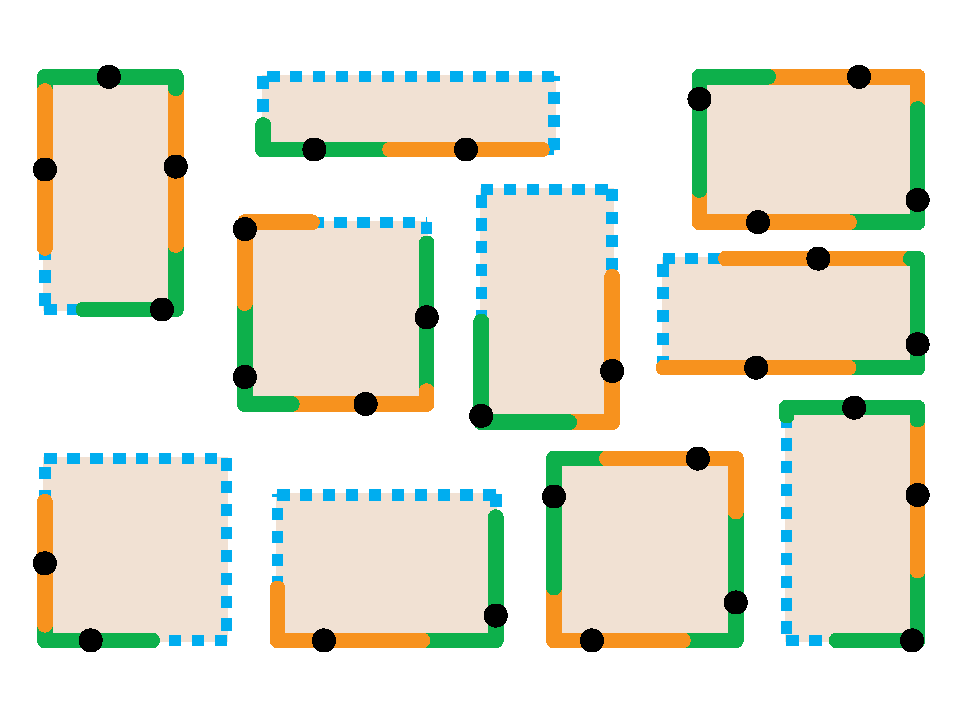
\includegraphics[keepaspectratio, scale=0.32]{./chapters/opg/figures/mpsc-example-eps-converted-to.pdf}
    \vspace*{-6mm}
    \caption[An example problem instance for MPSC]{\label{fig:opg-mpsc-example} 
    An example problem instance when $m = 10$ and $n = 30$. The black dots
		indicate deployed robot locations; the green and orange lines indicate
		the coverage.
    %We use blue dashed lines to show the gaps which do not need to be covered. 
    %The black filled circles illustrate final robot deployment locations, and 
    %the orange/green lines demonstrate individual robot covers. 
    %In this example, we use a different distribution to sample $len(P_i)$ due to 
    %cosmetic reasons.
		}
    \vspace*{-2mm}
\end{figure}

\begin{table}[ht!]
    \centering
		\vspace*{-4mm}
    \begin{footnotesize}
    \begin{tabular}{|c|c|c|c|c|c|c|} 
        \hline
        \diagbox{$m$}{$n$}       & $10^8  $ & $10^9   $ & $10^{10}$ & $10^{11}$ & $10^{12}  $ \\ \hline
        %\rule{0pt}{2.5ex} $10^3$ & $0.001 $ & $0.001  $ & $0.001  $ & $0.001  $ & $0.001    $ \\ \hline
        %\rule{0pt}{2.5ex} $10^4$ & $0.006 $ & $0.007  $ & $0.008  $ & $0.008  $ & $0.008    $ \\ \hline
        %\rule{0pt}{2.5ex} $10^5$ & $0.075 $ & $0.088  $ & $0.102  $ & $0.107  $ & $0.106    $ \\ \hline
        \rule{0pt}{2.5ex} $10^6$ & $1.152 $ & $1.442  $ & $1.508  $ & $1.652  $ & $1.617    $ \\ \hline
        \rule{0pt}{2.5ex} $10^7$ & $13.963$ & $17.281 $ & $18.796 $ & $20.354 $ & $20.627   $ \\ \hline
        \rule{0pt}{2.5ex} $10^8$ & NA       & $176.115$ & $223.186$ & $227.250$ & $230.000  $ \\ \hline
    \end{tabular}
		\end{footnotesize}
		% \vspace*{-3mm}
    \caption{\label{eval:opg-mpsc} \algoMRSimple~running time (seconds)}
		% \vspace*{-4mm}
\end{table}

%Recall that when the problem has multiple perimeters with single components, 
%each perimeter has exactly one segment and at most one gap. Our problem 
%generation procedure works as follows: given the number of perimeters $m$, we 
%first generate $m$ rectangles $\{R_1, \dots, R_m\}$ with $len(\partial R_i) = 1$ 
%for all $1 \leq i \leq m$, and then select a closed connected component $P_i$ 
%for each $R_i$. Here, $len(P_i)$ is uniformly randomly sampled from $(0, 1]$. 
%An example problem instance along with its optimal cover is shown in 
%~\ref{fig:mpsc-example}. The computation time of \algoMRSimple~under 
%different $m$ and $n$ is presented in Table.~\ref{eval:mpsc}. 
%\sh{Plots here. The constant factor in the $O(m(\log n + \log m) + \sum_{i} M_i)$ time 
%complexity is around $5 \times 10^{-8}$ seconds. }

For the case of a single perimeter with multiple components, a random 
polygon is generated on which $2q$ points are randomly sampled that 
yield $q$ segments (that form the perimeter) and $q$ gaps. An example 
instance and the optimal solution with $q=3$ and $n = 10$ is illustrated 
in ~\ref{fig:opg-spmc-example}. The computation time for various $q$ and 
$n$ combinations is given in Table~\ref{eval:opg-spmc}.
\begin{figure}[ht!]
    % \vspace*{-3mm}
    \centering
    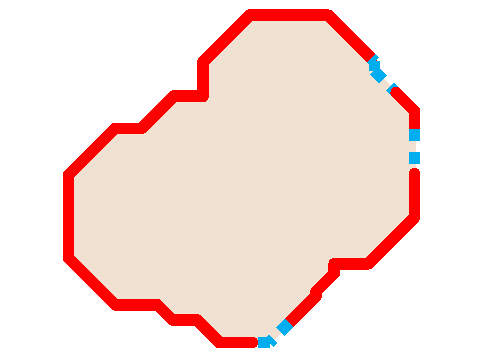
\includegraphics[keepaspectratio, scale=0.4]{./chapters/opg/figures/spmc-example-eps-converted-to.pdf}
    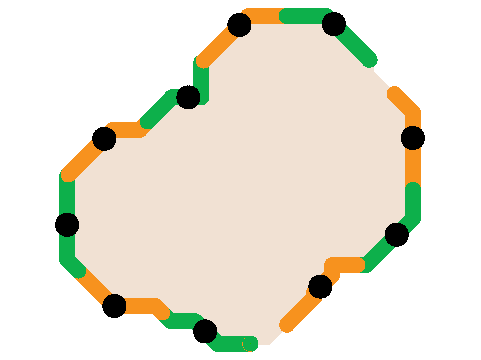
\includegraphics[keepaspectratio, scale=0.4]{./chapters/opg/figures/spmc-solution-eps-converted-to.pdf}
    % \vspace*{-3mm}
    \caption[Example OPG problem instance of SPMC]{\label{fig:opg-spmc-example} 
    An example problem instance when $q = 3$ and $n = 10$. In this case, the 
		optimal cover actually covers one gap.}
    % \vspace*{-4mm}
\end{figure}

\begin{table}[ht!]
    % \vspace*{-3mm}
    \footnotesize
    \centering
    \begin{tabular}{|c|c|c|c|c|c|c|} 
        \hline
        \diagbox{$q$}{$n$}       & $10^1   $ & $10^2   $ & $10^3  $  & $10^4   $ & $10^5$   \\ \hline       
        \rule{0pt}{2.5ex} $10^2$ & $0.013  $ & $0.015  $ & $0.016 $  & $0.016  $ & $0.017$  \\ \hline   
        \rule{0pt}{2.5ex} $10^3$ & $1.363  $ & $1.595  $ & $1.622 $  & $1.634  $ & $1.641$  \\ \hline   
        \rule{0pt}{2.5ex} $10^4$ & $159.404$ & $188.497$ & $210.492$ & $212.473$ & $212.780$\\ \hline   
    \end{tabular}
    \vspace*{-3mm}
    \caption{\label{eval:opg-spmc} \algoSRG~computation time (seconds)}
    \vspace*{-4mm}
\end{table}


%\subsubsection{\algoSRG} 
%To generate a problem of a single perimeter divided by interlaced segments and gaps, 
%we first create an arbitrary polygon $R$. Then, we uniformly randomly sample $2q$ points 
%on $\partial R$ to divide it into $q$ segments and $q$ gaps. 
%An example problem instance along with its optimal cover is shown in 
%~\ref{fig:spmc-example}. The computation time of 
%\algoSRG~under different $q$ and $n$ is presented in Table~\ref{eval:spmc}.

For multiple perimeters containing multiple components, $m$ polygons 
are created with $len(\partial R_i)$ randomly distributed in $[1, 10]$. 
For setting $q_i$, we fix a $q$ and let $q_i = q(0.5 + random(0, 1))$. 
Representative computation results of \algoMRG are listed in 
Table~\ref{eval:opg-mpmc}.
%whose perimeters' lengths are uniformly randomly sampled from interval $(1, 10)$. 
%The computation time under different $m$, $q$, and $n$ values are provided in Table~\ref{eval:mpmc}. 
%We observe that with the same $q$, $n$ parameters, the computation time is directly proportional to $m$.
\begin{table}[ht!]
    \vspace*{-2mm}
    \footnotesize
    \centering
    \begin{tabular}{|c|c|c|c|c|c|c|} 
        \hline
        \multirow{2}{*}{$q$} & \multirow{2}{*}{$n$} & \multicolumn{5}{|c|}{$m$} \\ \cline{3-7}
        \rule{0pt}{2.5ex} & & $10$ & $20$ & $30$ & $40$ & $50$ \\ \hline
        %\rule{0pt}{2.5ex} $10^1$ & $10^2$ & $ 0.015$ & $ 0.027$ & $ 0.039$ & $ 0.045$ & $ 0.054$ \\ \hline
        \rule{0pt}{2.5ex} $10^1$ & $10^3$ & $ 0.047$ & $ 0.063$ & $ 0.076$ & $ 0.091$ & $ 0.108$ \\ \hline
        %\rule{0pt}{2.5ex} $10^2$ & $10^2$ & $ 1.492$ & $ 2.784$ & $ 4.168$ & $ 5.404$ & $ 6.444$ \\ \hline
        \rule{0pt}{2.5ex} $10^2$ & $10^3$ & $ 2.191$ & $ 3.771$ & $ 5.523$ & $ 7.707$ & $ 9.369$ \\ \hline
        \rule{0pt}{2.5ex} $10^2$ & $10^4$ & $ 7.105$ & $ 9.619$ & $11.369$ & $12.760$ & $15.107$ \\ \hline
    \end{tabular}
    \vspace*{-3mm}
    \caption{\label{eval:opg-mpmc} \algoMRG~computation time (seconds)}
    \vspace*{-4mm}
\end{table}

Due to limited space, only selected essential performance data is 
presented here. More complete performance data and associate analysis 
can be found in the Appendix. 


\subsection{Two Applications Scenarios}
\noindent\textbf{Securing a perimeter}. As a first application, consider
a situation where a crime has just been committed at the Edinburgh 
Castle (see ~\ref{fig:opg-edinburgh}). The culprit remains in the confines 
of the castle but is mixed within many guests at the scene. As the 
situation is being investigated and suppose that the brick colored 
buildings are secured, guards (either personnel or a number of drones) may 
be deployed to ensure the culprit does not escape by climbing down the 
castle walls. Using \algoSRG, a deployment plan can be quickly computed 
given the amount of resources at hand so that each guard only needs to 
secure a minimum length along the castle walls. ~\ref{fig:opg-edinburgh} 
shows the optimal deployment plan for $15$ guards. 

\begin{figure}[ht]
	\vspace*{-2mm}
	\begin{center}
		\begin{overpic}[width=0.4\textwidth, tics=5]{./chapters/opg/figures/castle_15.eps}
			% \put(82,44){{\small $\W$}}
		\end{overpic}
	\end{center}
	\vspace*{-4.5mm}
	\caption[Optimal deployment of $15$ guards around walls of the Edinburgh Castle]
	{\label{fig:opg-edinburgh} Optimal deployment of $15$ guards around 
	walls of the Edinburgh Castle. The brick colored structures are buildings 
	that create gaps along the boundary.}
	%\vspace*{-3mm}
\end{figure}

\noindent\textbf{Fire monitoring}. In a second application, consider 
~\ref{fig:opg-forest} where a forest fire has just been put out in 
multiple regions. As there is still some chance that the fire may 
rekindle and spread, for prevention, a team of firefighters is to be 
deployed to watch for the possible spreading of the fire. Here, in 
addition to using \algoMRG to compute optimal locations for deploying 
the firefighters, we also generate minimum time trajectories for the 
firefighters to reach their target locations while avoiding going 
through the dangerous forests. This is done via solving a bottleneck 
assignment problem \cite{burkard1999linear}.
Note that the lake region creates gaps that cannot be traveled by the 
firefighters; this can be handled by making these gaps infinitely large. 
~\ref{fig:opg-forest} shows the optimal locations for $34$ firefighters. 
Animations of the deployment process and other test cases can be found 
in the accompanying video. 

\begin{figure}[ht]
	\vspace*{-2mm}
	\begin{center}
		\begin{overpic}[width=0.7\textwidth,tics=5]{./chapters/opg/figures/forest_solution.eps}
			%\put(82,44){{\small $\W$}}
		\end{overpic}
	\end{center}
	\vspace*{-4.5mm}
	\caption{\label{fig:opg-forest}  Optimal deployment of $34$ firefighters for 
	forest fire rekindling prevention.}
	\vspace*{-3mm}
\end{figure}




\subsection{Conclusion and Discussion}\label{section:opgext-opg-conclusion}
In this paper, we propose the \opg problem to model the allocation of 
large robotic swarms to cover complex 1D topological domains with 
optimality guarantees. For all variants under the \opg formulation 
umbrella, we have developed highly efficient algorithms for solving 
\opg exactly. In addition to rigorous proofs backed by formal analysis, 
extensive computational experiments further confirm the effectiveness of 
these algorithms. Moreover, practical relevance of \opg is demonstrated 
through the integration of \opg into realistic task (assignment) and motion 
planning scenarios. 

The study raises many additional interesting open questions; we mention 
a few here. 
%
First, the approach taken in this work is a {\em centralized} one where 
decision is made at the global level. It would be highly interesting to 
explore whether the same can be achieved with {\em decentralized} methods,
which have many advantages. For example, it may be the case that the 
gaps along the boundaries are not known {\em a priori} and must be measured
by the robots. In such cases, a centralized plan can be hard to come by. 
%
Second, as mentioned in Section~\ref{section:opg-problem}, the 
current \opg formulation assumes that the robots are confined to the 
boundaries $\partial \R$, which is one of many possible choices 
in terms of the robots' sensing and/or motion capabilities. In future study,
we plan to examine additional practical robot sensing and motion models. 
%
Third, as exact optimal algorithms are emphasized here, issues including 
uncertainty and robustness have not been touched in the current treatment, 
which are important elements when it comes to the deployment of a robotic 
swarm to tackle real-world challenges. 








\section{Perimeter Guarding with Heterogeneous Defenders}

\def\R{\mathcal R}
\def\C{\mathcal C}
\def\S{\mathcal S}
\def\P{\mathcal P}
\def\G{\mathcal G}
\def\W{\mathcal W}
\def\opg{{\sc {OPG}}\xspace}
\def\opglr{{\sc {OPG${}_{LR}$}}\xspace}
\def\opglrd{{\sc {D-OPG${}_{LR}$}}\xspace}
\def\opgmc{{\sc {OPG${}_{MC}$}}\xspace}

\newcommand{\argmin}[1]{\underset{#1}{\operatorname{arg}\,\operatorname{min}}\;}
\newcommand{\argmax}[1]{\underset{#1}{\operatorname{arg}\,\operatorname{max}}\;}

\def\twopart{\textbf{\textsc{Partition}}\xspace}
\def\tpart{\textbf{\textsc{$3$-Partition}}\xspace}
\def\ttkp{\textbf{\textsc{Knapsack}}\xspace}
\def\ttukp{\textbf{\textsc{Unbounded Knapsack}}\xspace}
\def\ttbp{\textbf{\textsc{Bin Packing}}\xspace}
\def\subsetsum{\textbf{\textsc{Subset Sum}}\xspace}

\subsection{Introduction}\label{sec:opgext-intro}
Consider the scenario where many mobile guards (or sensors) are to be deployed 
to patrol 
the perimeter of some 2D regions (~\ref{fig:opgext-ex}) against intrusion, where 
each guard may effectively cover a continuous segment of a region's boundary. 
When part of a boundary need not be secured, e.g., there may already be 
some existing barriers (the blue segments in ~\ref{fig:opgext-ex}), optimally 
distributing the robots so that each robot's coverage is minimized becomes 
an interesting and non-trivial computational task \cite{fenghangaoyu2019efficient}. 
It is established \cite{fenghangaoyu2019efficient} that, when the guards have 
the same capabilities, the problem, called the {\em optimal perimeter guarding} 
(\opg), resides in the complexity class P (polynomial time class), 
even when the robots must be distributed across many different boundaries. 

\begin{figure}[ht]
\begin{center}
\begin{overpic}[width=0.7\textwidth,tics=5]{chapters/opg-ext/figures/opg-eps-converted-to.pdf}
%\put(26,20){{\small $R_1$}}
%\put(20,39){{\small \textcolor{red}{$P_1$}}}
%\put(66,28){{\small $R_2$}}
%\put(54,40){{\small \textcolor{green}{$P_2$}}}
%\put(82,44){{\small $\W$}}
\end{overpic}
\end{center}
\caption[A scenario where boundaries of three (gray) regions must be secured]
{\label{fig:opgext-ex} A scenario where boundaries of three (gray) 
regions must be secured. Zooming in on part of the boundary of one 
of the regions (the part inside the small circle), portions of the 
boundary (the red segments) must be guarded while the rest (the 
blue dotted segments) does not need guarding. For example, the zoomed-in 
part of the boundary may be monitored by two mobile robots, each patrolling
along one of the green segments.}
\end{figure}

In this work, we investigate a significantly more general version of \opg 
where the mobile guards may be heterogeneous. More specifically, two 
formulations with different guarding/sensing models are addressed in our 
study. 
%
In the first, the number of available robots is fixed where robots of 
different types have a fixed ratio of capability (e.g., one type of 
robot may be able to run faster or may have better sensor). The guarding task 
must be evenly divided among the robots so that each robot, regardless of 
type, will not need to bear a too large coverage/capability ratio. This 
formulation is denoted as {\em optimal perimeter guarding with limited 
resources} or \opglr.
%
In the second, the number of robots is unlimited; instead, for each type, 
the sensing range is fixed with a fixed associated cost. The goal here is 
to find a deployment plan so as to fully cover the perimeter while minimizing 
the total cost. We call this the {\em optimal perimeter guarding with 
minimum cost} problem, or \opgmc. 

Unlike the plain vanilla version of the \opg problem, we establish that both 
\opglr and \opgmc are NP-hard when the number of robot types is part of the 
problem input. They are, however, at different hardness levels. \opglr is shown 
to be NP-hard in the strong sense, thus reducing the likelihood of finding a fully
polynomial time approximation scheme (FPTAS).
% solutions to even approximately solving it to arbitrary precision. 
Nevertheless, for the more practical case where the number of robot types 
is a constant, we show that \opglr can be solved using a pseudo-polynomial 
time algorithm with reasonable scalability. On the other hand, we show that 
\opgmc is weakly NP-hard through the establishment of a pseudo-polynomial 
time algorithm for \opgmc with arbitrary number of robot types. 
We further show that, when the number of robot types is fixed, \opgmc can be 
solved in polynomial time through a fixed-parameter tractable (FPT) approach.
This paragraph also summarizes the main contributions of this work. 

A main motivation behind our study of the \opg formulations is to address 
a key missing element in executing autonomous, scalable, and optimal robot 
deployment tasks. Whereas much research has been devoted to multi-robot 
motion planning \cite{ErdLoz86,arai2002advances} with great success, e.g., 
\cite{van2008reciprocal,smith2009monotonic,ayanian2010decentralized,turpin2014capt,
alonso2015multi,SolYu15}, existing results in the robotics literature appear 
to generally assume that a target robot distribution is already provided; the 
problem of how to effectively generate optimal deployment patterns is largely 
left unaddressed. It should be noted that control-based solutions to the 
multi-agent deployment problem do exist, e.g.,\cite{ando1999distributed,
jadbabaie2003coordination,cortes2004coverage,ren2005consensus,
schwager2009optimal,yu2012rendezvous,morgan2016swarm}, but the final solutions 
are obtained through many local iterations and generally do not come with 
global optimality guarantees. For example, in \cite{cortes2004coverage}, 
Voronoi-based iterative methods compute locally optimal target formations 
for various useful tasks. In contrast, this work, as well as 
\cite{fenghangaoyu2019efficient}, targets the scalable computation of globally optimal 
solutions. 
%To have an end-to-end system, the autonomous generation
%of deployment plan is clearly crucial. Where computational solutions for 
%\cite{alphago}. 
%\jy{Maybe mention alphago?}

As a coverage problem, \opg may be characterized as a 1D version 
of the well-studied Art Gallery problems  \cite{o1987art,shermer1992recent},
which commonly assume a sensing model based on line-of-sight 
visibility\cite{lozano1979algorithm}; the goal is to ensure that every point
in the  interior of a given region is visible to at least one of the deployed 
guards. Depending on the exact formulation, guards may be placed on 
boundaries, corners, or the interior of the region. Not surprisingly, Art
Gallery problems are typically NP-hard \cite{lee1986computational}. Other
than Art Gallery, 2D coverage problems with other sensing models, e.g., 
disc-based, have also been considered \cite{thue1910dichteste,hales2005proof,
drezner1995facility,cortes2004coverage,pavone2009equitable,
pierson2017adapting}, where some formulations prevent the overlapping 
of individual sensing ranges \cite{thue1910dichteste,hales2005proof} while 
others seek to ensure a full coverage which often requires intersection
of sensor ranges. 
%
In viewing of these studies, this study helps painting a broader landscape 
of sensor coverage research.

In terms of structural resemblance, \opglr and \opgmc share many similarities 
with {\em bin packing}  \cite{johnson1973near} and other related problems. 
In a bin packing problem, objects are to be selected to fit within bins of 
given sizes. Viewing the segments (the red ones in ~\ref{fig:opgext-ex}) as 
bins, \opg seeks to place guards so that the segments are fully contained in 
the union of the guards' joint coverage span. In this regard, \opg is a dual
problem to bin packing since the former must overfill the bins and the later 
cannot fully fill the bins. In the extreme, however, both bin packing and 
\opg converge to a \subsetsum \cite{karp1972reducibility} like problem where 
one seeks to partition objects into halves of equal total sizes, i.e., the 
objects should fit exactly within the bins. With an additional cost term, 
\opgmc has further similarities with the \ttkp problem \cite{lueker1975two}, 
which is weakly NP-hard \cite{dantzig1957discrete}.

The rest of the paper is organized as follows. In Section~\ref{sec:opgext-problem},
mathematical formulations of the two \opg variants are fully specified. In
Section~\ref{sec:opgext-hardness}, both \opglr and \opgmc are shown to be 
NP-hard. Despite the hardness hurdles, in Section~\ref{sec:opgext-algorithm}, 
multiple algorithms are derived for \opglr and \opgmc, including effective
implementable solutions for both. In Section~\ref{sec:opgext-application},
we perform numerical evaluation of selected algorithms and demonstrate 
how they may be applied to address multi-robot deployment problems. We 
discuss and conclude our study in Section~\ref{sec:opgext-conclusion}. Please
see \url{https://youtu.be/6gYL0_B3YTk} for an illustration of the problems 
and selected instances/solutions. 

\subsection{Preliminaries}\label{sec:opgext-problem}
Let $\W \subset \mathbb R^2$ be a compact (closed and bounded) 
two-dimensional workspace. There are  $m$ pairwise disjoint {\em 
	regions} $\R = \{R_1, \ldots, R_m\}$ where each region $R_i \subset \W$ 
is homeomorphic to the closed unit disc, i.e., there exists a continuous 
bijection $f_i: R_i \to \{(x, y) \mid x^2 + y^2 \le 1\}$ for all $1 \le 
i \le m$. For a given region $R_i$, let $\partial R_i$ be its (closed) 
boundary (therefore, $f_i$ maps $\partial R_i$ to the unit circle  
$\mathbb S^1$). With a slight abuse of notation, define $\partial \R 
= \{\partial R_1, \ldots, \partial R_m\}$. Let $P_i \subset \partial R_i$ 
be the part of $\partial R_i$ that is accessible, specifially, not blocked by 
obstacles in $\W$. This means that each $P_i$ is either a single closed 
curve or formed by a finite number of (possibly curved) line segments. 
Define  $\P = \{P_1, \ldots, P_m\} \subset \W$ as the {\em perimeter} 
of $\R$ which must be {\em guarded}. More formally, each $P_i$ is 
homeomorphic to a compact subset of the unit circle (i.e., it is 
assumed that the maximal connected components of $P_i$ are closed 
line segments). For a given $P_i$, each one of its maximal connected 
component is called a {\em perimeter segment} or simply a {\em segment}, 
whereas each maximal connected component of $\partial R_i \backslash P_i$ 
is called a {\em perimeter gap} or simply a {\em gap}. An example setting is 
illustrated in Fig.~\ref{fig:example-boundaries} with two regions. 
\definecolor{BrickRed}{RGB}{176, 50, 28}
\definecolor{ForestGreen}{RGB}{0, 155, 85}
\begin{figure}[ht]
	\begin{center}
		\begin{overpic}[width=0.7\textwidth,tics=5]
			{chapters/opg-ext/figures/example-boundaries-eps-converted-to.pdf}
			\put(26,20){{\small $R_1$}}
			\put(20,39){{\small \textcolor{BrickRed}{$P_1$}}}
			\put(66,28){{\small $R_2$}}
			\put(54,40){{\small \textcolor{ForestGreen}{$P_2$}}}
			%\put(79.6,18){{\small $h$}}
			\put(82,44){{\small $\W$}}
		\end{overpic}
	\end{center}
	\caption{\label{fig:example-boundaries} An example of a workspace $\W$ 
		with two regions $\{R_1, R_2\}$. Due to three {\em gaps} on $\partial R_1$, 
		marked as dotted lines within long rectangles, $P_1 \subset \partial R_1$ 
		has three {\em segments} (or maximal connected components); $P_2 = \partial 
		R_2$ has a single segment with no gap.}
\end{figure}

After deployment, some number of robots are to {\em cover} the perimeter 
$\P$ such that a robot $j$ is assigned a continuous closed subset $C_j$ 
of some $\partial R_i, 1 \le i \le m$. All of $\P$ must be {\em covered} 
by $\C$, i.e., 
%
$\bigcup_{P_i \in \P} P_i  \subset \bigcup_{C_j \in \C} C_j$,
%
which implies that elements of $\C$ need not intersect on their interiors. 
Hence, it is assumed that any two elements of $\C$ may share at most their 
endpoints. Such a $\C$ is called a {\em cover} of $\P$. Given a cover 
$\C$, for a $C_j \in \C$, let $len(C_j)$ denote its length (more formally, 
measure). 

To model heterogeneity of the robots, two models are explored in this
study. In either model, there are $t$ types of robots. In the first model,
the number of robots of each type is fixed to be $n_1, \ldots, n_t$ with 
$n = n_1 + \cdots + n_t$. For a robot $1 \le j \le n$, let $\tau_j$ denote 
its type. Each $1 \le \tau \le t$ type of robots has some 
level of {\em capability} or {\em ability} $a_{\tau} \in \mathbb Z^+$. We 
wish to balance the load among all robots based on their capabilities, 
i.e., the goal is to find cover $\C$ for all robots such that the quantity 
\[
\max_{C_j \in \C} \frac{len(C_j)}{a_{\tau_j}},
\]
which represents the largest coverage-capacity ratio, is minimized. 
We note that when all capacities are the same, e.g., $a_{\tau} = 1$ for 
all robots, this becomes the standard \opg problem studied in \cite{FenHanGaoYu19RSS}. 
We call this version of the perimeter guarding problem {\em optimal 
	perimeter guarding with limited resources} or \opglr. The formal 
definition is as follows.

\begin{problem}[Optimal Perimeter Guarding with Limited Resources 
	(\opglr)] Let there be $t$ types of robots. For each type $1\le \tau 
	\le t$, there are $n_{\tau}$ such robots, each having the same 
	capability parameter $a_{\tau}$. Let $n = n_1 + \cdots + n_t$. 
	Given the perimeter set $\P = \{P_1, \ldots, P_m\}$ of a set of 
	2D regions $\R =\{R_1, \ldots, R_m\}$, find a set of $n$ continuous 
	line segments $\C^* = \{C_1^*, \ldots, C_n^*\}$ such that $\C^*$ covers 
	$\P$, i.e., \begin{align}\label{eq:coverage}
	\bigcup_{P_i \in \P} P_i  \subset \bigcup_{C_j^* \in \C^*} C_j^*,
	\end{align}
	such that a $C_j^*$ is covered by robot $j$ of type $\tau_j$, and such that,
	among all covers $\C$ satisfying~\eqref{eq:coverage}, 
	\begin{align}\label{eq:objective}
	\C^* = \underset{\C}{\mathrm{argmin}} \max_{C_j \in \C} 
	\frac{len(C_j)}{a_{\tau_j}}.
	\end{align}
\end{problem}

Whereas the first model caps the number of robots, the second
model fixes the maximum coverage of each type of robot. That is, for 
each robot type $1 \le \tau \le t$, $n_{\tau}$, the number of robots of type $\tau$,
is unlimited as long as it is non-negative, but each such robot can only cover 
a maximum length of $\ell_{\tau}$. 
At the same time, using each such robot incurs a cost of $c_{\tau}$. The 
goal here is to guard the perimeters with the minimum total cost. We 
denote this problem {\em optimal perimeter guarding with minimum 
	cost} or \opgmc. 

\begin{problem}[Optimal Perimeter Guarding with Minimum Cost
	(\opgmc)] Let there be $t$ types of robots of unlimited quantities. 
	For each robot of type $1\le \tau \le t$, it can guard a length of 
	$\ell_{\tau}\in\mathbb{Z^+}$ with a cost of $c_{\tau}\in\mathbb{Z^+}$. Given the perimeter set
	$\P = \{P_1, \ldots, P_m\}$ of a set of 2D regions $\R =\{R_1, \ldots, 
	R_m\}$, find a set of $n = n_1 + \cdots + n_t$ continuous line segments 
	$\C^* = \{C_1^*, \ldots, C_n^*\}$ where $n_{\tau}$ such segments are 
	guarded by type $\tau$ robots, such that $\C^*$ covers $\P$, i.e., 
	\begin{align}\label{eq:coverage2}
	\bigcup_{P_i \in \P} P_i  \subset \bigcup_{C_j^* \in \C^*} C_j^*,
	\end{align}
	such that a $C_j^*$ is covered by robot $j$ of type $\tau_j$, i.e., 
	$C_j^* \le \ell_{\tau_j}$, and such that,
	among all covers $\C$ satisfying~\eqref{eq:coverage2}, 
	\begin{align}\label{eq:objective2}
	\C^* = \underset{\C}{\mathrm{argmin}} \sum_{1 \le \tau \le t} 
	n_{\tau}c_{\tau}.
	\end{align}
\end{problem}


\subsection{Computational Complexity for Variable Number of Robot Types}\label{sec:opgext-hardness}
We explore in this section the computational complexity of \opglr 
and \opgmc. Both problems are shown to be NP-hard with \opglr 
being strongly NP-hard. We later confirm that \opgmc is weakly 
NP-hard (in Section~\ref{sec:algorithm}).

\subsection{Strong NP-hardness of \opglr}\label{subsec:opglr-hardness}
When the number of types $t$ is a variable, i.e., $t$ is not a constant
and may be arbitrarily large,
% (but bounded by $n$), 
\opglr is shown to be NP-hard via the reduction from \tpart \cite{garey1975complexity}:

\vspace*{1mm}
\noindent
PROBLEM: \tpart\\
INSTANCE: A finite set A of $3m$ elements, a bound $B\in \mathbb{Z^+}$, 
% $S$ with $|S| = 3m$,
and a ``size'' $s(a)\in \mathbb{Z^+}$ for each $a\in A$,
such that each $s(a)$ satisfies $B/4 < s(a) <B/2$ and $\sum_{a\in A} s(a) = mB$.\\
QUESTION: Is there a partition of $S$ into $m$ disjoint subsets $S_1, 
\ldots, S_m$ such that for $1\leq i\leq m$, 
$\sum_{a\in S_i} s(a) = B$?
\vspace*{1mm}

%In a \tpart instance, let $\sum_{s \in S} s = B$ and for all $b \in B$, 
%$1/4 < b <  1/2$. Under such conditions, \tpart remains strongly 
%NP-hard \cite{garey1979computer}. We will use this version of the \tpart problem. We mention here that we use fractional values for 
%the elements of $B$ to avoid adding additional variables; this is fine 
%as long as we restrict the involved numbers to be rationals. 
\tpart is shown to be NP-complete in the strong sense\cite{GarJoh79}, 
i.e., it is NP-complete even when all numeric inputs are bounded by a polynomial 
of the input size. 

For the reduction, it is more convenient to work with a decision 
version of the \opglr problem, denoted as \opglrd. In the \opglrd 
problem, $a_{\tau}$ is the actual length robot type $\tau$ covers. 
That is, the coverage length of a robot is fixed. The \opglrd problem 
is specified as follows. 

\vspace*{1mm}
\noindent
PROBLEM: \opglrd\\
INSTANCE: $t$ types of robots where there are $n_{\tau}$ robots for 
each type $1 \le \tau \le t$; $n = n_1 + \cdots + n_t$. A robot of 
type $\tau$ has a coverage capacity $a_{\tau}$. A set of perimeters 
$\P = \{P_1, \ldots, P_m\}$ of a set of 2D regions 
$\R =\{R_1, \ldots, R_m\}$.\\ 
QUESTION: Is there a deployment of $n$ disjoint subsets $C_1, \ldots, C_n$
of $\{\partial R_1, \ldots, \partial R_m\}$ such that 
$P_1 \cup \ldots \cup P_m \subset C_1 \cup \ldots \cup C_n$, where
$C_j$ is a continuous segment for all $1 \le j \le n$, and for each 
$1 \le j \le n$, there is a unique robot whose type $\tau$, $1 \le \tau 
\le t$ satisfies $a_{\tau} \ge len(C_j)$?
\vspace*{1mm}

\begin{theorem}\label{t:opglr-hard}
	\opglr is strongly NP-hard. 
\end{theorem}
\begin{proof}
	A polynomial reduction from \tpart to \opglrd is constructed
	by a restriction of \opglrd. Given a \tpart instance with former notations,
	we apply several restrictions on \opglrd: {\em (i)} there are $3m$ types of robot
	and there is a single robot 
	for each type, i.e., $n_{\tau} = 1$ for $1 \le \tau \le t$, so $n=t=3m$ 
	{\em (ii)} the $3m$ capacities $a_1, \ldots, a_{3m}$ are set to be equal to
	$s(a)$ for each of the $3m$ elements $a\in A$, and {\em (iii)} 
	there are $3m$ perimeters and each perimeter $P_i$ is continuous and
	$len(P_i)=B$ for all $1 \le i \le m$.

	% \begin{comment}
	% In this proof, we work with a further restriction of \opglrd: {\em (i)}
	% there is a single robot for each type, i.e., $n_{\tau} = 1$ for $1 
	% \le \tau \le t$, and {\em (ii)} each perimeter $P_i$ is continuous and
	% %$len(P_i)$ is the same for all $1 \le i \le m$.
	
	% $len(P_i) = B$ for all $1 \le i \le m$.
	% Given a \tpart instance with $\sum_{b_i \in B} b = q$ and $1/4 \le b 
	% \le  1/2$ for all $b_i \in B$, let the corresponding \opglrd instance 
	% have $q$ perimeters, each with a single segment with the same length 
	% $L$. Let there be $3q$ robots, each with a type $1 \le \tau \le 3q$ 
	% and capability parameter $a_{\tau} = b_{\tau} \in B$. The restricted
	% \opglrd problem instance asks a question similar to the \tpart problem: 
	% is there a partition of the robots such that each perimeter of length 
	% $1$ is covered by three robots (notice that it is impossible to reach 
	% a total capacity of $1$ with fewer or more than $3$ robots)? 
	% \end{comment}

	% \begin{comment}
	% We make some rudimentary observations regarding the \opglrd instance 
	% and the related \opglr instance. Since all $q$ perimeters are of length 
	% $L$ each and the total capability of the robots is $q$, the objective 
	% \eqref{eq:objective} cannot be lower than $\frac{qL}{q} = L$, which is 
	% achieved only when each perimeter is covered by robots with total 
	% capability parameter of $1$. Then, because of the requirement $1/4 < 
	% a_{\tau} < 1/2$, if the best possible solution to the related \opglr 
	% instance is to be realized, each perimeter must be covered by exactly 
	% three robots; otherwise, the total capability cannot sum up to $1$. 
	% \end{comment}
	
	With the setup, the reduction proof is straightforward. Clearly, the 
	\tpart instance admits a partition of $A$ into $S_1, \ldots, 
	S_m$ such that $\sum_{a \in S_i} s(a) = B$ for all $1\leq i\leq m$ 
	if and only if a
	valid depolyment exists in the corresponding \opglrd instance. 
	It is clear that the reduction from \tpart to 
	\opglrd is polynomial (in fact, linear). Based on the 
	reduction and because \tpart is strongly NP-hard, so is \opglrd 
	%(by Lemma 4.1 of \cite{garey1975complexity}) 
	and \opglr.
\end{proof}

\begin{remark}
	One may also reduce weakly NP-hard problems, e.g., \twopart
	\cite{karp1972reducibility}, to \opglr for variable number of robot 
	types $t$. Being strongly NP-hard, \opglr is unlikely to admit pseudo-polynomial 
	time solutions for variable $t$. This contrasts with a later result 
	which provides a pseudo-polynomial time algorithm for \opglr for 
	constant $t$, as one might expect in practice where robots have limited 
	number of types. We also note that Theorem~\ref{t:opglr-hard} continues 
	to hold for a single perimeter with multiple segments, each 
	having a length $B$ in previous notation, separated by ``long'' gaps. Obviously, 
	\opglrd is in NP, thus rendering it NP-complete. 
\end{remark}

\subsection{NP-hardness of \opgmc}
The minimum cost \opg variant, \opgmc, is also NP-hard, which may be 
established through reduction from the \subsetsum problem 
\cite{karp1972reducibility}:

\vspace*{1mm}
\noindent
PROBLEM: \subsetsum \\
INSTANCE: A set $B$ with $|B| = n$ and a weight function $w: B \to 
\mathbb Z^+$, and an integer $W$.\\ 
QUESTION: Is there a subset $B' \subseteq B$ such that $\sum_{b \in B'} 
w(b) = W$?
\vspace*{1mm}

\begin{theorem}\label{t:opgmc-hard}
	\opgmc is NP-hard. 
\end{theorem}
\begin{proof}
	Given a \subsetsum instance, we construct an \opgmc instance with a 
	single perimeter containing a single segment with length $L$ to be 
	specified shortly. Let there be $t=2n$ types of robots. For $1 \le i 
	\le n$, let robot type $2i-1$ have $\ell_{2i-1} = c_{2i-1} = 
	w(b_i) + (2^{n + 1} + 2^i)W'$ and let robot type $2i$ have $\ell_{2i} 
	= c_{2i} = (2^{n + 1} + 2^i)W'$. Here, $W'$ can be any integer number no less than 
	$\sum_{b\in B} w(b)$. Set $L = W + (n2^{n+1} + 2^n + \ldots 
	+ 2^1)W'$. We ask the ``yes'' or ``no' decision question of whether there 
	are robots that can be allocated to have a total cost no more than $L$ 
	(equivalently, equal to $L$, as the cost density $c_\tau/l_\tau$
	is always $1$).
	
	Suppose the \subsetsum instance has a yes answer that uses a subset
	$B' \subseteq B$. Then, the \opgmc instance has a solution with cost $L$ 
	that can be constructed as follows. For each $1 \le i \le n$, a single 
	robot of type $2i - 1$ is taken if $b_i \in B'$. Otherwise, a single 
	robot of type $2i$ is taken. This allocation of robots yields a total 
	length and cost of $L$. 
	
	For the other direction, we first show that if the \opgmc instance 
	is to be satisfied, it can only use a single robot from type $2i-1$ 
	or $2i$ for all $1 \le i \le n$. First, if more than $n$ robots are 
	used, then the total cost exceeds $(n + 1)2^{n+1}W' > L$ as $W\leq W'$.
	% because $W' + (2^n + \ldots + 2)W' < 2^{n+1}W'$. 
	Similarly, if less than $n$ 
	robots are used, the total length is at most 
	$(n-1)2^{n+1}W'+(2^{n+1}-1)W'+ W' < L$. 
	Also, to match the $(2^n + \ldots + 2)W'$ part of the cost, exactly one robot 
	from type $2i-1$ or $2i$ for all $1 \le i \le n$ must be taken. 
	Now, if the \opgmc decision instance has a yes answer, if a robot 
	of type $2i -1$ is used, let $b_i \in B$ be part of $B'$, which 
	constructs a $B'$ that gives a yes answer to the \subsetsum instance.
\end{proof}
% add this citation because the proof the hardness probably comes from it
\begin{remark}
	It is also clear that the decision version of the \opgmc problem is 
	NP-complete. The \subsetsum is a weakly NP-hard problem that admits 
	a pseudo-polynomial time algorithm \cite{dantzig1957discrete}. 
	As it turns out, \opgmc, which shares similarities with \subsetsum
	and \ttkp (in particular, \ttukp \cite{ukphardness}), though NP-hard, 
	does admit a pseudo-polynomial time algorithm as well. 
\end{remark}

\begin{comment}
In concluding the section, we note that we have not determined the 
hardness for the case with constant number of robot types. There are 
some recent evidence that such problems may not be as hard as when 
the number of robot types is a fixed input parameter 
\cite{goemans2014polynomiality}.
\end{comment}



% \section{Exact Algorithm via Dynamic Programming}\label{sec:algorithm}
\subsection{Exact Algorithms for \opglr and \opgmc}\label{sec:opgext-algorithm}
In this section, we describe three exact algorithms for solving the two 
variations of the \opg problem. First, we present a pseudo-polynomial time
algorithm for \opglr when the number of robot types, $t$, is a fixed constant. 
Given that \opglr is strongly NP-hard, this is in a sense a best possible 
solution. 
%
For \opgmc, in addition to providing a pseudo-polynomial algorithm for 
arbitrary $t$, which confirms that \opgmc is weakly NP-hard, we also provide
a polynomial time approximation scheme (PTAS). We then further show the 
possibility of solving \opgmc in polynomial time when $t$ is a fixed constant. 
We mention that our development in this section focuses on the single 
perimeter case, i.e., $m = 1$, as the generalization to arbitrary $m$ is 
straightforward using techniques described in \cite{fenghangaoyu2019efficient}. With this in mind, 
we also provide the running times for the general setting with arbitrary $m$ 
but refer the readers to \cite{fenghangaoyu2019efficient} on how these running times can be derived. 

For presenting the analysis and results, for the a perimeter $P$ that we work 
with, assume that it has $q$ perimeter segments $S_1, \ldots, S_q$ that need 
to be guarded; these segments are separated by $q$ gaps $G_1, \ldots, G_q$. 
For $1 \le i, i' \le q$, define $S_{i\sim i'} = S_i \cup G_i \cup S_{i+1} \cup \ldots 
\cup G_{i'-1} \cup S_{i'}$ where $i'$ may be smaller than $i$ (i.e., $S_{i\sim i'}$
may wrap around $G_q$),
For the general case with $m$ perimeters, assume that a perimeter $P_i$ has
$q_i$ segments. 
\begin{comment}
\jy{A paper, or anything with some level of complexity to digest, should be 
hierarchical. So, at the beginning of a section, it is good to explain a bit 
of what will be covered so a reader will have an idea of the structure of 
the section.}
\end{comment}

\subsection{Pseudo-Polynomial Time Algorithm for \opglr with Fixed Number
of Robot Types}
\SetKw{Continue}{continue}
\SetKw{True}{true}
\SetKw{False}{false}
\SetKwComment{Comment}{\%}{}
\SetKwInOut{Input}{Input}
\SetKwInOut{Output}{Output}
\def\inc{{\sc Inc}\xspace}
\def\knapsack{\textbf{\textsc{Knapsack}}\xspace}
\def\opglrfeasible{{\sc OPG-lr-Feasible}\xspace}
\def\opgmcdp{{\sc OPG-mc-DP}\xspace}
We set to develop an algorithm for \opglr for arbitrary $t$, the number of robot 
types; the algorithm runs in pseudo-polynomial time when $t$ is a constant. 
At a higher level, our proposed algorithm works as follows. First, our main effort 
here goes into deriving a feasibility test for \opglrd as defined in 
Section~\ref{subsec:opgext-opglr-hardness}. With such a feasibility test, we can then 
find the optimal $\frac{len(C_j)}{a_{\tau_j}}$ in \eqref{eq:opgext-opg-objective} via binary search.
Let us denote the optimal value of $\frac{len(C_j)}{a_{\tau_j}}$ as $\ell^*$. 

\subsubsection{Feasibility Test for \opglrd} The feasibility test for \opglrd 
essentially tries different candidate $\ell$ to find $\ell^*$. Our implementation uses 
ideas similar to the pseudo-polynomial time algorithm for the \knapsack problem which
is based on dynamic programming (DP). In the test, we work with a fixed starting point on 
$P$, which is set to be the counterclockwise end point of a segment $S_i$, $1 \le i \le q$. 
Essentially, we maintain a $t$ dimensional array $M$ where dimension $\tau$
has a size of $n_{\tau} +1$. An element of the array, $M[n_1']\ldots[n_t']$, holds the 
maximal distance starting from $S_i$ that can be covered by $n_1'$ type 1 robots, 
$n_2'$ type 2 robots, and so on. The DP procedure \opglrfeasible($i, \ell$), outlined in 
Algorithm~\ref{algo:opgext-opglrd}, incrementally builds this array $M$. For convenience,
in the pseudo code, $M[\vec{x}]$ denotes an element of $M$ with $\vec{x}$ being 
a $t$ dimensional integer vector. 

\begin{algorithm}
	\DontPrintSemicolon
	% \KwData{$n_1, n_2, \cdots, n_k$ robots, $l_1, l_2, \cdots, l_n$ coverage distance}
	\KwData{$n_1, \ldots, n_t$, $a_1, \ldots, a_t$,
		$S_1, \ldots, S_q$, $G_1, \ldots, G_q$}
	\KwResult{\True or \False,  indicating whether $S_1, \ldots, S_q$ can be covered}
	%\Begin{
		Initialize $M$ as a $t$ dimensional array with dimension $\tau$ having a size of $n_{\tau} + 1$;\;
		$\ell_{\tau} \leftarrow a_{\tau}\ell$ for all $1\le \tau \le t$;\;
		\For{$ \vec{x} \in [0, n_1]\times\dots\times[0,n_t]$}{
            $M[\vec{x}]\leftarrow 0$;\;
			\For{$j = 1$ \KwTo $t$}{
				\lIf{$\vec{x}_j = 0$}{\Continue;}
				$\vec{x'}\leftarrow\vec{x}$; $\vec{x'}_j \leftarrow \vec{x'}_j - 1$;\;
				$M[\vec{x}]\leftarrow max$($M[\vec{x}]$, \inc($M[\vec{x'}], \ell_j$));\;
			}
			% \For{$i_2 \leftarrow 1$ \KwTo $n_2$}{
			% $\cdots$\;
			% \For{$i_k \leftarrow 1$ \KwTo $n_k$}{
			% $DP[i_1][i_2]\cdots[i_k]\leftarrow$ min(Increment($DP[i_1-1][i_2]\dots[i_k],\cdots,l_1$), Increment($DP[i_1][i_2-1]\dots[i_k], l_2$), $\cdots$, Increment($DP[i_1][i_2]\cdots[i_k-1],l_k$)\;
			% }
			% }
		}
		\Return{$M[n_1]\ldots[n_t] \ge len(S_{i\sim {i-1}})$};
	%}
	\caption{\opglrfeasible($i, \ell$)}\label{algo:opgext-opglrd}
\end{algorithm}

In Algorithm~\ref{algo:opgext-opglrd}, the procedure \inc($L, \ell$) checks how much of the 
perimeter $P$ can be covered when an additional coverage length $\ell$ is added, 
assuming that a distance of $L$ (starting from some $S_i$) is already covered. An 
illustration of how \inc($L, \ell$) works is given in ~\ref{fig:opgext-inc}.
 

\begin{figure}[ht]
	\begin{center}
		\begin{overpic}[width=0.7\textwidth,tics=5]
			{chapters/opg-ext/figures/inc-eps-converted-to.pdf}
			\put(26,10){{\small $L$}}
			\put(61,10){{\small $\ell$}}
			\put(30,1){{\small \textsc{Inc}($L$, $\ell$)}}
		\end{overpic}
	\end{center}
    \caption[Illustration of a solution]{\label{fig:opgext-inc}Suppose starting from the fixed left point, a 
		length of $L$ on the boundary is successfully guarded by a group of 
		robots. Then, a robot with coverage capacity $\ell$ is appended to 
		the end of the group of robots to increase the total guarded distance. 
		In the figure, the added additional capacity $\ell$ can fully cover 
		the third red segment plus part of the third (dashed) gap. Because 
		there is no need to cover the rest of the third gap, 
		\textsc{Inc}($L$, $\ell$) extends to the end of the gap.}
\end{figure}

%Denote procedure $Inc(L, \ell)$ as the length of boundary successfully guarded from $L$ using a continuous segment length of $\ell$.

%It is straightforward to see that Algorithm~\ref{algo:opglrd} has a running 
%time of $O(t\Pi_{i=1}^{t} (n_i+1))$ if we populate $M$ gradually.

By simple counting, the complexity of the algorithm is
$O(q\cdot t\cdot\Pi_{\tau=1}^{t} (n_{\tau}+1))$. However, the amortized
complexity of \inc($\cdot$) for each $\tau$ is $O(q+n_{\tau})$; the algorithm thus 
runs in $O(t\cdot\Pi_{{\tau}=1}^{t}(n_{\tau}+1)+q\cdot\sum_{{\tau}=1}^{t} 
\Pi_{{\tau'}\neq {\tau}} (n_{\tau'} +1))$, 
which is pseudo-polynomial for fixed $t$. After trying every possible starting 
position $i$ with \opglrfeasible($i, \ell$), for a fixed candidate $\ell$, 
\opglrd is solved in $O(q \cdot t\cdot\Pi_{{\tau}=1}^{t}(n_{\tau}+1) + 
q^2\cdot\sum_{{\tau}=1}^{t} \Pi_{{\tau'}\neq {\tau}} (n_{\tau'} +1))$.

\subsubsection{Solving \opglr using Feasibility Test for \opglrd}
Using \opglrfeasible($i, \ell$) as a subroutine to check feasibility for a given $\ell$, 
bisection can be applied over candidate $\ell$ to obtain $\ell^*$. For completing 
the algorithm, one needs to establish when the bisection will stop (notice that, 
even though we assume that $a_\tau \in \mathbb{Z^+}$, for each $1\leq \tau \leq t$, $\ell^*$ need not be 
an integer). 

To derive the stop criterion, we note that given the optimal $\ell^*$, there must 
exist some $S_{i\sim i'}$ that is ``exactly'' spanned by the allocated robots.
That is, assume that $S_{i\sim i'}$ is covered by $n_1'$ of type $1$ robots
and $n_2'$ of type $2$ robots, and so on, then 
\begin{align}\label{eq:opgext-exact}
\ell^* = \frac{len(S_{i\sim i'})}{\sum_{1 \le \tau \le t} a_{\tau}\cdot n_{\tau}'}.
\end{align}

\eqref{eq:opgext-exact} must hold for some $S_{i\sim i'}$ because if not, the solution 
is not tight and can be further improved. Therefore, the bisection process for 
locating $\ell^*$ does not need to go on further after reaching a certain granularity\cite{fenghangaoyu2019efficient}.
%$1/\sum_{1 \le \tau \le t} a_{\tau}\cdot n_{\tau}$. 
With this established, using 
similar techniques from \cite{fenghangaoyu2019efficient} (we omit the technical detail as it is quite 
complex but without additional new ideas beyond beside what is already covered 
in \cite{fenghangaoyu2019efficient}), we could prove that the full algorithm needs 
no more than $O(q\log(\sum_{\tau}n_{\tau}+q)$ calls to \opglrfeasible($i, \ell$).
%$O(t\Pi_{i=1}^{t}(n_i+1)+q\sum_{i=1}^{t} \Pi_{j\neq i} (n_j +1))$
This directly implies that \opglr also admits a pseudo-polynomial algorithm for fixed $t$.
% \sw{The complexity here is the decision version of single perimeters}
\subsubsection{Multiple Perimeters}
Also using techniques developed in \cite{fenghangaoyu2019efficient}, the single perimeter 
result can be readily generalized to multiple perimeters. We omit the mechanical
details of the derivation and point out that the computational complexity in this case becomes
$\tilde{O}( (m-1)\cdot((\Pi_{\tau=1}^t n_\tau) / \max_\tau n_\tau)^2 + 
\sum_{k=1}^{m} (t\cdot q_k\cdot \Pi_{{\tau}=1}^{t}(n_{\tau}+1)+
q_k^2\sum_{{\tau}=1}^{t} \Pi_{{\tau'}\neq {\tau}} (n_{\tau'} +1)))$.
% \sw{the complexity here is for decision version of multiple perimeters, starting
%  from a specific starting point}
%\jy{I updated the formula as it seems to be wrong. Also changed $r$ to $m$.}

\subsection{Polynomial Time Algorithm for \opgmc with Fixed Number of Robot Types}
%\subsection{$OPG_{MC}$}
The solution to \opgmc will be discussed here. A method based on DP 
will be provided first, which leads to a polynomial time algorithm for a 
fixed number of robot types and a pseudo-polynomial time algorithm when the number 
of robot types is not fixed. For the latter case, a polynomial time approximation 
scheme (PTAS) will also be briefly described.
\subsubsection{Dynamic Programming Procedure for \opgmc}
\def\sol{{\sc Sol}}
\def\presol{{\sc PreSolve}}
When no gaps exist, the optimization problem becomes a covering 
problem as follows. Let $c_{\tau}$, $\ell_{\tau}$, $n_{\tau}$ correspond to the cost, 
coverage length, and quantity of robot type ${\tau}$, respectively, and let total 
length to cover be $L$. We are to solve the optimization problem
\begin{align}\label{eq:opgext-ip}
    \min \sum_{\tau} c_{\tau} \cdot n_{\tau} \quad s.t.\, \quad
    \sum_{\tau} \ell_{\tau} \cdot n_{\tau} \geq L, n_{\tau}\geq 0.
\end{align}

Let the solution to the above integer programming problem be \sol($L$).
Notice that, for $S_{i\sim i'}:=\{S_i,\ G_i, \dots, 
G_{i'-1}, S_{i'}\}$, the minimum cost cover is by either: {\em (i)} 
covering the total boundary without skipping any gaps, 
%
or {\em (ii)} skipping or partially covering some gap, for example $G_k, 
i \le k \le j-1$.
%
In the first case, the minimum cost is exactly \sol$(\lceil len(S_{i\sim(i+k)}\rceil)$.
%
In the second case, the optimal structure for the two subsets of perimeter 
segments $S_{i\sim k}$ and $S_{(k+1)\sim j}$ still holds. This means that the 
continuous perimeter segments $S_{i\sim j}$ can be divided into two parts, 
each of which can be treated separately. This leads to a DP approach for \opgmc.
With $M[i][j]$ denoting the minimum cost to cover $S_{i\sim j}$, the DP recursion 
is given by
\[
	\scalebox{0.93}{$M[i][j] = \min(\textit{\sol}(\lceil len(S_{i\sim j})\rceil), \displaystyle\min_k(M[i][k]+M[k+1][j]))$}
\]

The DP procedure is outlined in Algorithm~\ref{alg:opgext-opgmc}. In the pseudo code, 
it is assumed that indices of $M$ are modulo $q$, e.g., $M[2][q+1] 
\equiv M[2][1]$. $tmp$ is a temporary variable. 
\begin{comment}
\jy{Generally mathematicians and theoretical computer scientists use 
	$\ell_1, \ldots, \ell_t$ instead of $\ell_1, \ell_2, \ldots, \ell_t$. The later is more 
	redundant. Also, normally we use ldots instead of cdots. I changed $C$ to $M$ since 
    $C$ is used elsewhere. I changed $==$ to $=$ to save space.}
\end{comment}
\begin{algorithm}
    \DontPrintSemicolon
    % \KwData{$n_1, n_2, \cdots, n_k$ robots, $l_1, l_2, \cdots, l_n$ coverage distance}
    \KwData{$\ell_1, \dots, \ell_t$, $c_1, \ldots, c_t$,
    	$S_1, \ldots, S_q$, $G_1, \ldots, G_q$}
    \KwResult{$c^*$, the minimum covering cost}
   %\Begin{
    $M \leftarrow$ a $q\times q$ matrix; $c^* \leftarrow \infty$; \;
    \For{$k \leftarrow 0$ \KwTo $q-1$}{
        \For{$i\leftarrow 1 $ \KwTo $q$}{
            $tmp \leftarrow\ $\sol$(\lceil len(S_{i\sim(i+k)}) \rceil)$; \;
            \For{$j\leftarrow i$ \KwTo $i+k-1$}{
                $tmp \leftarrow \min(tmp, M[i][j] + M[j+1][i+k])$;
            }
            $M[i][i+k] \leftarrow c$;\;
            \lIf{$k = q-1$}{$c^* \leftarrow \min(c^*, M[i][i+k])$;}
        }
    }
    \Return{$c^*;$}
    %}
    \caption{\opgmcdp}
    \label{alg:opgext-opgmc}
\end{algorithm}

\subsubsection{A Polynomial Time Algorithm for \opgmc for a Fixed Number of Robot Types}
We mention briefly that, by a result of Lenstra \cite{lenstra1983integer}, the optimization problem 
~\eqref{eq:opgext-ip} is in P (i.e., polynomial time) when $t$ is a constant. The running time of 
the algorithm \cite{lenstra1983integer} is however exponential in $t$. 

\subsubsection{A Pseudo-polynomial Time Algorithm for Arbitrary $t$}
As demonstrated in the hardness proof, similarities exist between \opg and the \knapsack 
problem. The connection actually allows the derivation of a pseudo-polynomial time algorithm
for arbitrary $t$. To achieve this, we use a routine to pre-compute \sol($L$), called 
\presol(), which is itself a DP procedure similar to that for the \knapsack problem. The 
pseudo code of \presol() is given in Algorithm~\ref{algo:opgext-presol}.
\presol() runs in time $O(t\cdot\lceil len(\partial R)\rceil))$. Overall, 
Algorithm~\ref{alg:opgext-opgmc} then runs in time $O(q^3+t\cdot\lceil len(\partial R\rceil))$.
%\jy{Is this running time correct?}

\begin{algorithm}
	\DontPrintSemicolon
	\KwData{$\ell_1, \ldots, \ell_t$, $c_1, \ldots, c_t$}
	\KwResult{A lookup table for retrieving \sol($L$)}
	%\Begin{
		$I_{max} = \lceil len(\partial R)\rceil$; \Comment{\small $I_{max}$ is an integer.}
		$M' \leftarrow$ an array of length $I_{max} + 1$; 
		$M'[0]\leftarrow 0$;\;
		\For{$L \leftarrow$ $1$ \KwTo $I_{max}$}{
			$M'[L]\leftarrow \infty$; \;
			\For{${\tau}\leftarrow 1$ \KwTo $t$}{
				$tmp \leftarrow (L<\ell_{\tau}\ ?\ 0\ :\ M'[L-\ell_{\tau}]) + c_{\tau}$;\;
				$M'[L] \leftarrow min(M'[L], tmp)$;\;
			}
		}
		\Return{$M'$}
	%}
	\caption{{\sc PreSolve}}\label{algo:opgext-presol}
\end{algorithm}

%After the preprocessing, 
%the Solution(L) is just an access of $Sol[L]$. 
%Algorithm \ref{alg:opgmc} still applies and the only modification is a simple replacement of 
%\sol($L$) with $Sola[L]$. This make the complexity of \ref{alg:opgmc} drop to $O(q^3)$.
% \begin{algorithm}
%     \DontPrintSemicolon
%     % \KwData{$n_1, n_2, \cdots, n_k$ robots, $l_1, l_2, \cdots, l_n$ coverage distance}
%     \KwData{$l_1, l_2, \cdots, l_k$ coverage distance, $c_1, c_2,\cdots,c_k$ deployment cost}
%     \KwResult{Minimum cost for covering the perimeter}
%     \Begin{
%     $DP \leftarrow$ 1-D array length of L with data initialized to $\infty$\;
%     $DP[0]\leftarrow 0 $\;
%     $Result\leftarrow \infty$\;
%     \For{$l \leftarrow 0$ \KwTo $L$}{
%     \If{$DP[l] = \infty$}{  \Continue\;}
%     \For{$i \leftarrow 1$ \KwTo $k$}{
%     $nextEnd \leftarrow $Increment($l, l_i$)\;
%     $DP[nextEnd] = \min(DP[nextEnd], DP[l]+c_i)$\;
%     \If{$nextEnd\geq L$}{Result$\leftarrow \min(Result,DP[nextEnd])$}
%     }
%     }
%     \Return{Result}
%     }
%     \caption{} 
% \end{algorithm}
With the establishment of a pseudo-polynomial time algorithm for \opgmc, we  
have the following corollary. 
\begin{corollary}
	\opgmc is weakly NP-hard. 
\end{corollary}

\subsubsection{FPTAS for Arbitrary $t$}
When the number of robot types is not fixed, Lenstra's algorithm\cite{lenstra1983integer} or 
its variants no longer run in polynomial time. We briefly mention that, 
%via a linear time transformation, 
by slight modifications of a FPTAS for \ttukp problem from \cite{ibarra1975fast}, a FPTAS 
for \opgmc can be obtained that runs in time $O(q^3 + q^2 \cdot \frac{t}{\epsilon^3})$, 
where $(1+\epsilon)$ is the approximation ratio for both \opgmc and ~\eqref{eq:opgext-ip}. 

\subsubsection{Multiple Perimeters} For \opgmc, when there are multiple 
perimeters, e.g., $P_1, \ldots, P_m$, a optimal solution can be obtained 
by optimally solving \opgmc for each perimeter $P_i$ individually and 
then put together the solutions. 



%\section{Experimental Studies}\label{sec:experiments}
%\input{texs/05-experiments}

\subsection{Performance Evaluation and Applications}\label{sec:opgext-application}
In this section, we provide examples illustrating the typical 
optimal solution structures of \opglr and \opgmc computed by 
our DP algorithms. Using an application scenario, solutions to 
\opglr and \opgmc are also compared. Then, computational 
results from extensive numerical evaluations are presented, 
confirming the effectiveness of these algorithms. The 
implementation is done using the Python and all 
computations are performed on an Intel(R) Core(TM) i7-7700 CPU@3.6GHz 
with 16GB RAM. 

\subsection{Basic Optimal Solution Structure}
Fig.~\ref{fig:opgext-opglrm} shows the typical outcome of solving an \opglr 
instance with two perimeters ($m = 2$) for two types of robots with 
$n_1 = 3, a_1 = 5$, and $n_2 = 5, a_2 = 8$. 
%That is, the second type of robots is more capable than the first type. 
In the figure, the red segments are parts of the two perimeters that 
must be guarded. The three orange (resp., five green) segments across 
the two perimeters indicate the desired coverage regions of the three 
(resp., five) type $1$ (resp., type $2$) robots. These coverage regions 
correspond to the optimal solution returned by the DP algorithm. As 
may be observed, the optimal solution is somewhat complex with robots 
of both types on each of the two perimeters; a gap on the second boundary 
also gets covered. The coverage lengths for a robot type are generally 
different; this is due to adjustments that shrink some robots' coverage. 
For example, the first perimeter has a very short orange cover because 
the corresponding perimeter segment is short and gaps around it need 
not be covered (The adjustment procedure is also shown in the video). 
\begin{figure}[!ht]
    \centering
    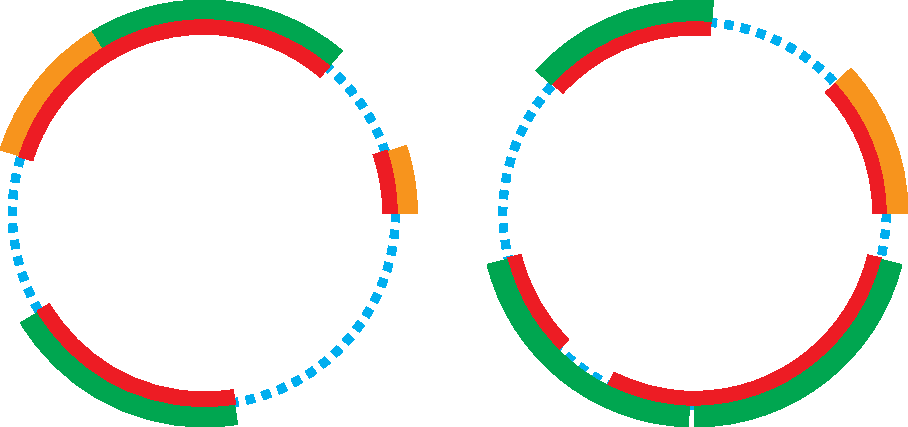
\includegraphics[scale = 0.6]{chapters/opg-ext/figures/mopglr_shrink-new-eps-converted-to.pdf}
    \caption{An \opglr problem and an associated optimal solution. The 
		problem has two perimeters and $t = 2$ with $n_1$=3, $n_2$=5, 
		$a_1$=5, $a_2$=8. The boundaries are shown as circles for ease of 
		illustration.
		%, which does not affect the computation or the solution.
		}
		\label{fig:opgext-opglrm}
\end{figure}

Shifting our attention to \opgmc, Fig.~\ref{fig:opgext-opgmc} illustrates the 
structure of an optimal solution to a problem with three types of robots 
with capacities and costs being $\ell_1=11, c_1=2$, $\ell_t=30, 
c_2=4$, and $\ell_3=55, c_3=7$, respectively. In this case, the majority 
of the deployed robots are of type $2$ with $\ell_2=30, c_2=4$. Only one 
type $1$ and one type $3$ robots are used. The four perimeter segments are 
covered by three robot groups. 
%
%To clearly illustrate the solution structure, the combined coverage of each 
%robot group runs beyond the counterclockwise direction of the corresponding 
%segments being covered (e.g., the counterclockwise end of the orange segment 
%is inside a gap). 
%
The only type $3$ robot guards (the purple segment) across two different 
perimeter segments. Coverage length adjustment is also performed to avoid 
the unnecessary coverage of some gaps. 

\begin{figure}[!ht]
    \centering
    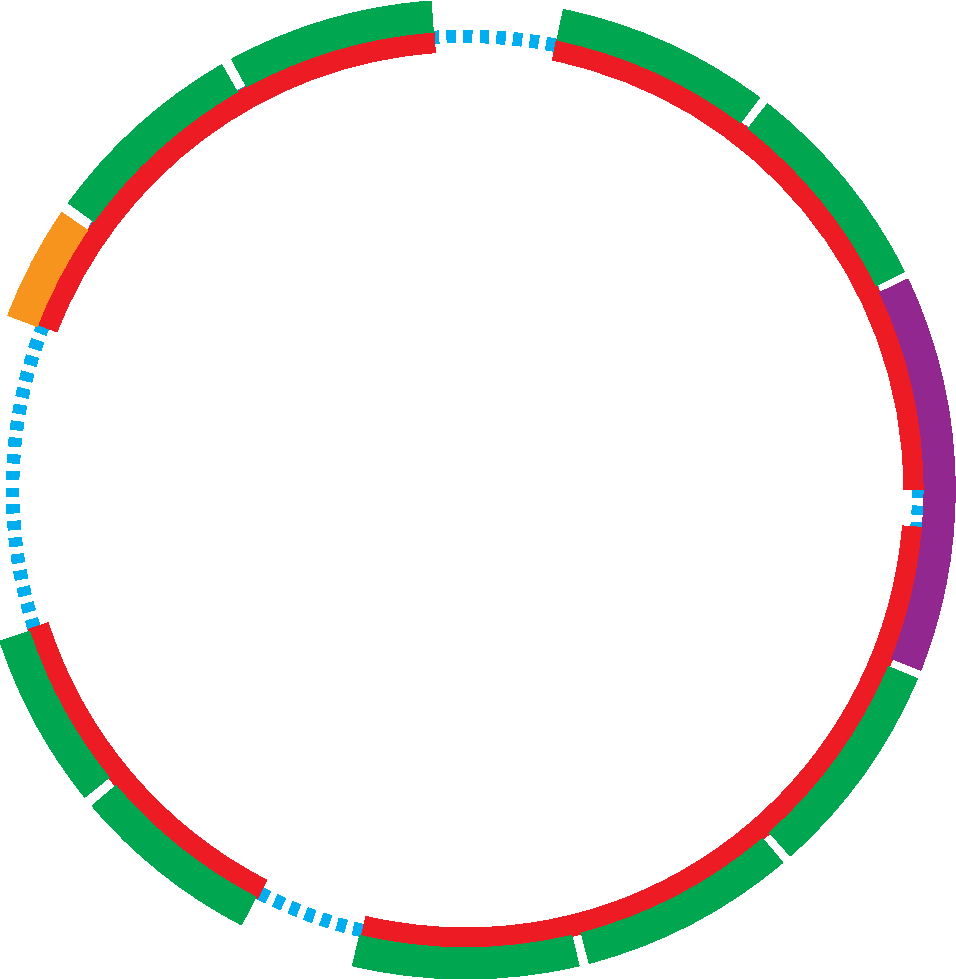
\includegraphics[scale = 0.4]{chapters/opg-ext/figures/opgmc-new-t-eps-converted-to.pdf}
    \caption{An \opgmc problem and an associated optimal solution. The 
		problem has four (red) perimeter segments and three types of robots
		with $\ell_1=11, c_1=2$ (orange), $\ell_t=30, c_2=4$ (green), 
		and $\ell_3=55, c_3=7$ (purple), respectively.}
		\label{fig:opgext-opgmc}
\end{figure}

\subsection{A Robotic Guarding and Patrolling Application}
In this subsection, as a potential application, the DP algorithms for 
\opglr and \opgmc are employed to solve the problem of securing the 
perimeter of the Edinburgh castle, an example used in 
\cite{FenHanGaoYu19RSS}. As shown in Fig.~\ref{fig:opgext-castle} (minus 
the orange and green segments showing the solutions), the central 
region of the Edinburgh castle has tall buildings on its boundary 
(the blocks in brick red); these parts of the boundary are the gaps 
that do not need guarding. In the figure, the top sub-figure shows 
the optimal solution for an \opglr instance and an \opgmc instance with 
a total of $11$ robots. The bottom sub-figure is a slightly updated 
\opgmc instance with slightly higher $c_2$. 
\begin{figure}[!ht]
    \centering
    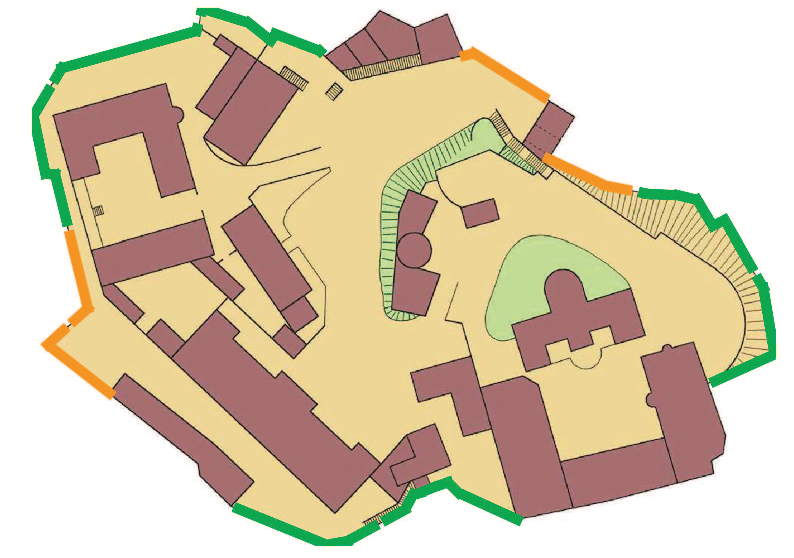
\includegraphics[scale = 0.5]{chapters/opg-ext/figures/opglr-castle-thin-eps-converted-to.pdf}
    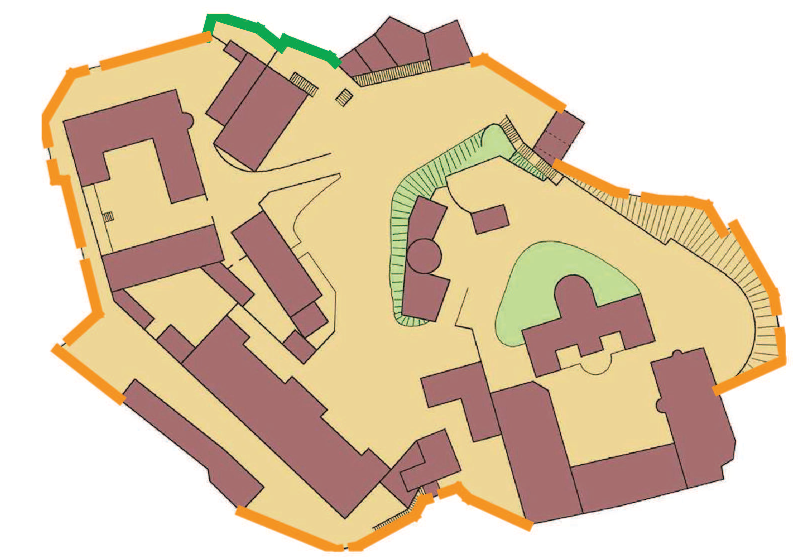
\includegraphics[scale = 0.5]{chapters/opg-ext/figures/opgmc-castle-thin-eps-converted-to.pdf}
    \caption{[left] \opglr solution with $n_1 = 4, n_2 = 7, 
		c_1:c_2 = 2:3$ and \opgmc solution with $\ell_1 = 150, 
		c_1 = 100, \ell_2 = 225, c_2 = 145$, and total boundary $3058$. Cost 
		of \opgmc solution is $1415$.
		[right] \opgmc solution with $\ell_1 = 150, c_1 = 100, \ell_2 = 
		225, c_2 = 155$. Cost of solution ($13$ type $1$, $1$ type $2$) is 
		$1455$.
		%
		In both solutions, covers by type $1$ (resp., 
		type $2$) robots are shown in orange (resp., green).
		%, which does not affect the computation or the solution.
		}
		\label{fig:opgext-castle}
\end{figure}

It can be observed that the results, while having non-trivial structures, 
make intuitive sense. For the top sub-figure, solutions to both \opglr 
and \opgmc (because robot with larger capacity is slightly lower in 
relative cost) use mainly higher capacity robots to cover longer perimeter 
segments and use the lower capacity robots mostly fillers. The solution 
covers a small gap at the bottom. For the bottom sub-figure, while only 
small changes are made to the cost, because the longer segment is more 
expensive to use now, the first type of robot is used mainly. 

\subsection{Computational Performance}
With Section~\ref{sec:opgext-algorithm} fully establishing the correctness and 
asymptotic complexity of the pseudo-polynomial time algorithms, here, the 
running time of these algorithms are experimentally evaluated. In doing 
so, the main goal is demonstrating that, despite the hardness of \opglr 
and \opgmc, the proposed algorithms could solve the target problems under 
reasonably broad settings in a scalable way. For results presented in 
this subsection, each data point is an average over 10 randomly generated 
instances. 

The first two numerical evaluations (Table~\ref{tab:opgext-opglr} and 
Table~\ref{tab:opgext-mopglr}) focus on the running times of the pseudo-polynomial 
time algorithms for \opglr over single and multiple perimeters, 
respectively. In these two tables, $t$ and $q$ are the number of types 
and the number of segments, respectively. For each type $\tau$, a 
capacity ($a_{\tau}$) is randomly sampled as an integer between $1$ and 
$100$, inclusive. The number of robots available for each type ($n_{\tau}$) 
is sampled uniformly between $5$ and $15$, inclusive. For the multiple 
perimeters case, the parameter $m$ represents the number of perimeters for 
a given instance.

For the single perimeter case (Table~\ref{tab:opgext-opglr}), the results show 
that the pseudo-polynomial time algorithm is effective for up to five 
types of robots, for dozens of robots. We expect a more efficient 
(e.g., C++ based) implementation should be able to effectively handle 
up to five types of robots with the total number of robots being around 
a hundred, on a typical PC. This is likely sufficient for many practical 
applications which have limited types and numbers of robots. Since the 
algorithm has exponential dependency on $t$, it becomes less efficient 
for larger $t$ as expected.  

\begin{table}[htbp]
	\centering
	\begin{tabularx}{\columnwidth}{|c|X|X|X|X|X|X|}
		\hline
%		\renewcommand{\arraystretch}{0.99}
		\diagbox{$t$}{$q$}&  \quad 5 &   \quad 10 &\quad 20& \quad 30 & \quad 40&\quad 50 \\
		\hline
		\renewcommand{\arraystretch}{1.05}
		2&0.022 &0.044 &0.131 &0.208 &0.326 &0.516 \\\hline
        3&0.281 &0.714 &1.670 &2.577 &4.107 &4.708 \\\hline
        4&5.504 &16.07 &41.68 &71.55 &109.9 &138.9 \\\hline
        5&29.53 &75.60 &243.6 &443.4 &528.0 &725.0 \\\hline
	\end{tabularx}
	\caption{Running time in seconds used by the DP algorithm for \opglr over 
	a single perimeter.
	}
	\label{tab:opglr}
\vspace*{-1mm}
\end{table}

Table~\ref{tab:opgext-mopglr} illustrates the running time of the DP algorithm for 
\opglr over multiple perimeters. As can be readily observed, the impact of 
the number of perimeters $m$ on the running time is relatively small; the 
number of robot types is still the determining factor for running time. In 
this case, our proposed solution is effective for $t$ up to $4$ and starts to 
slow down a robot types become larger than $4$. 
\begin{table}[htbp]
	\centering
	\renewcommand{\arraystretch}{1.05}
    \begin{tabularx}{\columnwidth}{|c|X|X|X|X|X|X|}
        \hline
        {\multirow{2}{*}{\diagbox{$m$}{$q$}} }&\multicolumn{2}{c|}{10}&\multicolumn{2}{c|}{20}&\multicolumn{2}{c|}{30} \\
        \cline{2-7}
         &\,\,\,$t$=3 & $\,\,\,t$=4& $\,\,\,t$=3 & $\,\,\,t$=4& \,\,\,$t$=3  & \,\,\,$t$=4\\
        \hline
        2&3.148 &133.2 &7.077 &198.4 &10.33 &260.0 \\\hline
        3&4.828 &194.1 &10.125 &290.6 &15.52 &376.7 \\\hline
        4&6.131 &256.8 &12.485 &381.3 &19.75 &514.3 \\\hline
        5&7.622 &321.7 &15.355 &476.2 &24.31 &605.8 \\\hline
    \end{tabularx}
    \caption{Running time in seconds used by the DP algorithm for \opglr over multiple perimeters.}
    \label{tab:mopglr}
\vspace*{-1mm}
\end{table}

Table~\ref{tab:opgext-opgmc} provides performance evaluation of \opgmcdp. Since 
there is no difference between single and multiple perimeters for \opgmc,
only problems with single perimeters are attempted. Here, for each robot 
type, the cost is an integer randomly sampled between $1$ and $20$, and 
the capacity is computed as five times the cost plus a random integer 
between $1$ and $20$. In the table, $L = \partial R$, the total length 
of the entire boundary. 
%
Given \opgmc's lower computational complexity, the DP algorithm, 
\opgmcdp, can effectively deal with over a few hundred types of robots 
with ease. 
\begin{table}[!ht]
	\centering
	\renewcommand{\arraystretch}{1.04}
    \begin{tabularx}{\columnwidth}{|c|X|X|X|X|X|X|}
        \hline
        \multirow{2}{*}{\diagbox{$t$}{$L$}} & 
        \multicolumn{2}{c|}{$10^2$}&\multicolumn{2}{c|}{$10^4$} &\multicolumn{2}{c|}{$10^6$} \\
        \cline{2-7}
        &$q$=20&$q$=50&$q$=20&$q$=50&$q$=20&$q$=50\\
        \hline
        3&0.006 &0.064 &0.041 &0.098 &3.040 &3.144 \\\hline
        10&0.005 &0.066 &0.094 &0.155 &9.423 &9.409 \\\hline
        30&0.009 &0.070 &0.261 &0.320 &26.10 &28.59 \\\hline
        100&0.014 &0.077 &0.910 &0.969 &91.28 &93.20 \\\hline
        300&0.030 &0.091 &2.652 &2.938 &275.6 &270.7 \\\hline
    \end{tabularx}
    \caption{Running time in seconds used by \opgmcdp algorithm.}
    \label{tab:opgext-opgmc}
\end{table}
\vspace*{-1mm}
\begin{comment}
    Application 1: for a single large region with a perimeter that may be viewed as straight line segments locally, we want to deploy multiple types of robots with different sensing radius. The goal is to ensure full coverage of the perimeter. Both problems formulations can be used. 

This also raises a related problem: what if we want to use discs to cover perimeter when a segment cannot be treated as straight lines? Can we also do tiling somehow? 

Another question: if we just use the same number of robots as used in an optimal cover to do a random feasible tiling, what would be the worst sub-optimality ratio? 

Application 2:  a multi-region application?
\end{comment}

\subsection{Conclusion and Discussions}\label{sec:opgext-conclusion}
In this section, we investigate two natural models of optimal perimeter 
guarding using heterogeneous robots, where one model (\opglr) limits 
the number of available robots and the second (\opgmc) seeks to 
optimize the total cost of coverage. 

These formulations have many potential applications. One application 
scenario we envision is the deployment of multiple agents or robots 
as ``emergency responders'' that are constrained to travel on the 
boundary. An optimal coverage solution will then translate to minimizing 
the maximum response time anywhere on the perimeter (the part that 
needs guarding). The scenario applies to \opg, \opglr, and \opgmc. 

Another application scenario is the monitoring of the perimeter 
using robots with different sensing capabilities. A simple heterogeneous 
sensing model here would be robots equipped with cameras with different 
resolutions, which may also be approximated as discs of different radii. 
The model makes sense provided that the region to be covered is much 
larger than the sensing range of individual robots and assuming that the 
boundary has relatively small curvature as compared to the inverse of the 
radius of the smallest sensing disc of the robots. For boundary with 
relatively small curvature, our solutions would apply well to the sensing 
model by using the diameter of the sensing disc as the 1D sensing range. 
As the region to be covered is large, covering the boundary will require
much fewer sensors than covering the interior. 


On the computational complexity 
side, we prove that both \opglr and \opgmc are NP-hard, with \opglr 
directly shown to be strongly NP-hard. This is in stark contrast to 
the homogeneous case, which admits highly efficient low polynomial 
time solutions \cite{fenghangaoyu2019efficient}. The complexity study also 
establishes structural similarities between these problems and 
classical NP-hard problems including \tpart, \ttkp, and \subsetsum.

On the algorithmic side, we provide methods for solving both \opglr 
and \opgmc exactly. For \opglr, the algorithm runs in pseudo-polynomial 
time in practical settings with limited types of robots. In 
this case, the approach is shown to be computationally effective. 
For \opgmc, a pseudo-polynomial time algorithm is derived for the 
general problem, which implies that \opgmc is weakly NP-hard. In 
practice, this allows us to solve large instances of \opgmc. We 
further show that a polynomial time algorithm is possible for 
\opgmc when the types of robots are fixed. 

With the study of \opg \cite{fenghangaoyu2019efficient} for homogeneous and 
heterogeneous cases, some preliminary understanding has been 
obtained on how to approach complex 1D guarding problems. 
Nevertheless, the study so far is limited to {\em one-shot} settings
where the perimeters do not change. In future research, we would like 
to explore the more challenging case where the perimeters evolve 
over time, which requires the solution to be dynamic as well. Given 
the results on the one-shot settings, we expect the dynamic setting
to be generally intractable if global optimal solutions are desired, 
potentially calling for iterative and/or approximate solutions. 

We recognize that our work 
does not readily apply to a visibility-based sensing model, which is also 
of interest. Currently, we are also exploring covering of the interior
using range-based sensing. As with the OPG work, we want to push for 
optimal or near-optimal solutions when possible.
\vspace*{-1mm}


    
\chapter{Optimal Set Guarding with 2D disc-based sensing model}
\thispagestyle{myheadings}

% text of this chapter goes here
\def\R{\mathbf{R}}
\def\C{\mathcal C}
% \def\S{\mathcal S}
% \def\P{\mathcal P}
% \def\G{\mathcal G}
\def\W{\mathcal W}

\def\opt{\textsc{OPT}\xspace}

\def\osgt{\textsc{OSG${}_{\mathrm{2D}}$}\xspace}

\def\opg{\textsc{OPG}\xspace}
\def\opgt{\textsc{OPG${}_{\mathrm{2D}}$}\xspace}
\def\orgt{\textsc{{ORG}${}_{\mathrm{2D}}$}\xspace}
\def\dopgt{\textsc{{D-OPG}${}_{\mathrm{2D}}$}\xspace}
\def\dorgt{\textsc{{D-ORG}${}_{\mathrm{2D}}$}\xspace}


In this chapter, we consider the problem of using mobile robots equipped 
with range sensors to guard (1D) perimeters or (2D) regions. Given 
a bounded polygonal one- or two-dimensional set to be secured, 
and $k$ mobile sensing robots where robot $i$'s sensor covers a circular region of 
radius $r_i$, we seek deployment of the robots so that $\max r_i$ is 
minimized. That is, we would like to minimize the maximum single-sensor 
coverage across all sensors. We denote this multi-sensor coverage problem 
under the umbrella term {\em optimal set guarding with 2D sensors}, or 
\osgt.\footnote{The subscript is placed here to distinguish our setup 
from the \opg problem studied in \cite{fenghangaoyu2019efficient}, which assumes 
a 1D sensing model.} The specific problem for guarding
perimeters (resp., regions) is denoted as {\em optimal perimeter 
(resp., region) guarding with 2D sensors}, abbreviated as \opgt (resp., 
\orgt). Beside direct relevance to sensing, surveillance, and monitoring 
applications using mobile sensors \cite{batalin2002spreading,
cortes2004coverage,fenghangaoyu2019efficient}, \osgt applies to other robotics
related problem domains, e.g., the deployment of ad-hoc mobile wireless 
networks \cite{correll2009ad,gil2012communication}, in which case an 
optimal solution to \osgt provides a lower bound on the guaranteed network 
strength over the targeted 2D region. 

\section{Introduction}\label{sec:osg-intro}
In this paper, we consider the problem of using mobile robots equipped 
with range sensors to guard (1D) perimeters or (2D) regions. Given 
a bounded polygonal one- or two-dimensional set to be secured, 
and $k$ mobile robots where robot $i$'s sensor covers a circular region of 
radius $r_i$, we seek a deployment of the robots so that $\max r_i$ is 
minimized. That is, we would like to minimize the maximum single-sensor 
coverage across all sensors. We denote this multi-sensor coverage problem 
under the umbrella term {\em optimal set guarding with 2D sensors}, or 
\osgt.\footnote{The subscript is placed here to distinguish our setup 
from the \opg problem studied in \cite{fenghangaoyu2019efficient}, which assumes 
a 1D sensing model.} The specific problem for guarding
perimeters (resp., regions) is denoted as {\em optimal perimeter 
(resp., region) guarding with 2D sensors}, abbreviated as \opgt (resp., 
\orgt). Beside direct relevance to sensing, surveillance, and monitoring 
applications using mobile sensors \cite{batalin2002spreading,
cortes2004coverage,fenghangaoyu2019efficient}, \osgt applies to other robotics
related problem domains, e.g., the deployment of ad-hoc mobile wireless 
networks \cite{correll2009ad,gil2012communication}, in which case an 
optimal solution to \osgt provides a lower bound on the guaranteed network 
strength over the targeted 2D region. 
%\sw{more accurate to use 2OPT+epsilon and OPT+epsilon, the epsilon is addditive}

\begin{figure}[ht]
    \centering
		\vspace*{2mm}
    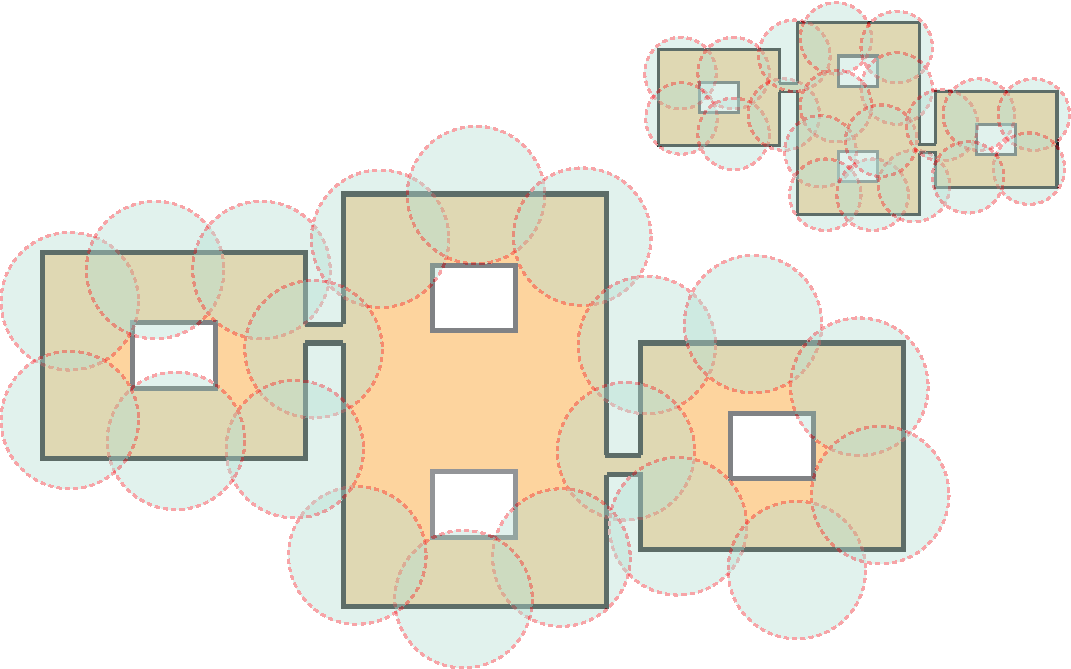
\includegraphics[width=\columnwidth]{chapters/osg/figures/example-0-eps-converted-to.pdf}
		\vspace*{1mm}
    \caption{An illustration of the \osgt setup and sample solutions.
		[center] The background shows the footprint of a building, e.g., an 
		apartment  complex. Scenarios may arise that a dangerous criminal 
		might be hiding in the building and we would like to closely monitor 
		the outer boundary of the building.	For the setting, the shaded 
		discs provide a	near-optimal cover with minimum radii for $20$ 
		mobile sensors that fully encloses the outer perimeter, computed 
		using algorithms presented in this work with optimality guarantees. 
		[upper right] A near-optimal solution for guarding the interior of
		the building footprint minus the four holes.}
    \label{fig:example0}
\end{figure}
As a summary of the study, on the side of computational complexity, we 
establish that \opgt is hard to approximate within a factor of 
$1.152$
even when the perimeter is a simple closed polygonal chain whose length
is bounded by the input size, through a reduction from 
vertex cover on planar bridgeless $3$-regular graphs.
%
A unique property of our reduction is that it shows the inapproximability gap
remains when each sensor can cover at most two disjoint perimeter 
segments. 
%
The proof also shows that \orgt is at least as hard to approximate. 
Therefore, no polynomial time algorithm may exist that solves \osgt to 
better than the $1.152$-optimal lower bound, unless P$\,=\,$NP. 
%
On the algorithmic side, we begin by providing an efficient $(1+\varepsilon)$
approximation algorithm
for a specific class of \opgt problems in which each mobile 
sensor must cover a continuous perimeter segment. This implies that the 
aforementioned inapproximability result on \opgt under the 
two-disjoint-segment sensing model is tight. 
%
For the general \osgt problem, we first describe a polynomial time 
$(2+\varepsilon)$ approximation algorithm as a reasonable approximability 
upper bound. 
%
Then, an integer linear programming (ILP) model is devised that allows 
the fast computation of highly optimal solutions for fairly large 
problem instances. 
%\jy{Maybe an example here on the scale of problems that we can solve and how fast.}
%
Results described in this paragraph, together with the introduction 
of \osgt as a practical multi-robot deployment problem focusing on global 
optimality, constitute the main contributions of this work. 

As an intermediate result toward showing the hardness of the simple polygon
coverage problem, we also supply a hardness proof of vertex cover 
on planar bridgeless\footnote{That is, the deletion of any edge does not disconnect 
the graph.} $3$-regular graphs, which may be of independent interest. 

\textbf{Related work}. Our work on optimal perimeter and region guarding 
draws inspiration from a long line of multi-robot coverage planning and 
control research, e.g., \cite{cortes2004coverage,martinez2007motion,
schwager2009optimal,pavone2009equitable,schwager2009decentralized,
pierson2017adapting}. 
%
In an influential body of work on coverage control \cite{cortes2004coverage,
martinez2007motion}, a gradient based iterative method is shown to drive 
one or multiple mobile sensors to a locally optimal configuration with 
convergence guarantees. 
%
Whereas \cite{cortes2004coverage,martinez2007motion} assume that the 
distribution of sensory information is available {\em a priori}, it is 
shown that such information can be effectively learned 
\cite{schwager2009decentralized}. 
%
Subsequently, the control method is further extended to allow the 
coverage of non-convex and disjoint 2D domains \cite{schwager2009optimal} 
and to work for mobile robots with varying sensing or actuation capabilities
\cite{pierson2017adapting}. 
%
In contrast to these control-based approaches, which produce iterative 
locally optimal solutions, \osgt emphasizes the direct computation of 
globally optimal deployment solutions and supports arbitrarily shaped
bounded (1D) perimeters and (2D) regions.

Recently, the problems of globally optimally covering perimeters using 
one-dimensional sensors have been studied in much detail 
\cite{fenghangaoyu2019efficient,fengyu2020RAL}. It is shown that when the sensors 
are homogeneous, the optimal deployment of sensors can be computed 
very efficiently, even for highly complex perimeters \cite{fenghangaoyu2019efficient}.
On the other hand, the problem becomes immediately intractable, sometimes
strongly NP-hard, when sensors are heterogeneous \cite{fengyu2020RAL}. 
Our research is distinct from \cite{fenghangaoyu2019efficient,fengyu2020RAL} in that 
we employ a (two-dimensional) range sensing model and work on the coverage 
of both perimeters and regions, which has much broader applicability. 

As pointed out in \cite{cortes2004coverage,schwager2009decentralized}, 
distributed sensor coverage, as well as \osgt, has roots in the study 
of the facility location optimization problem 
\cite{weber1929theory,drezner1995facility}, which examines the selection 
of facility (e.g., warehouses) locations that minimize the cost of delivery 
of supplies to spatially distributed customers. In theoretical computer 
science and operations research, these are known as the $k$-center, 
$k$-means, and $k$-median clustering problems \cite{har2011geometric}, 
the differences among which are induced by the cost structure. Our 
investigation of \osgt benefits from the vast literature on 
the study of $k$-center clustering and related problems, e.g., 
\cite{feder1988optimal,hochbaum1985best,gonzalez1985clustering,daskin2000new,shamos1975closest}.
%
These clustering problems are in turn related to packing 
\cite{hales2005proof}, tiling \cite{thue1910dichteste}, and the 
well-studied art gallery problems \cite{o1987art,shermer1992recent}.

\textbf{Organization}. The rest of the paper is organized as follows. 
In Section~\ref{sec:problem}, we introduce the \osgt formulation. 
Section~\ref{sec:complexity} is devoted to establishing that \osgt is 
hard to approximate to better than $1.152$-optimal, providing a theoretical
lower bound. In Section~\ref{sec:algo}, focusing on the upper bound, 
we describe algorithms that for \osgt and the special \opgt variant 
where a sensor is allowed to cover a continuous perimeter segment.
In Section~\ref{sec:expr}, we benchmark the algorithms and illustrate two 
potential applications. We discuss and conclude the work in Section~\ref{sec:conc}.





\section{Preliminaries}\label{sec:osg-problem}
% We define .... 
Let $\mathcal{W}\subset \mathbb{R}^2$ be a 
% compact (i.e., closed and bounded) 
polygonal workspace, which may contain one or multiple connected components. 
A {\em critical subset} of $\mathcal{W}$ needs to be guarded by $k$ 
%\sw{jumpping from $r_i$ to inditinguishable}
indistinguishable point guards with range sensing capabilities. For 
example, the workspace may be a forest reserve and the critical subset 
may be its boundary. Or, the workspace may be a high-security facility, 
e.g., a prison, and the critical subset the prison yard. The $i$th 
guard, $1\le i\le k$, located at $c_i \in \mathbb{R}^2$, can monitor a circular 
area of radius $r_i$ centered at $c_i$ with $r_i$ being a variable. For 
example, the guard may be a watchtower equipped with a vision sensor 
that can detect intruders. As the watchtower's altitude increases, 
its sensing range also increases; but its monitoring quality will 
decrease at the same time due to resolution loss. In this study, we seek 
to compute the optimal strategy to deploy these $k$ guards so that the 
required sensing range, $\max_i r_i$, could be minimized. 

More formally, we model a connected component of $\W$ as some 2D polygonal region
containing zero or more simple polygonal obstacles. 
For a bounded set $D \subset \mathbb{R}^2$, we define
\begin{equation*}
size(k, D) = \min_{c_1, \dots, c_k\in \mathbb{R}^2}\ \max_{p\in D}\ \min_{1\leq i\leq k} \lVert c_i - p \rVert_2 
\end{equation*}
and use $B(c, r)$ to denote the disc of radius $r$ centered at a point $c 
\in \mathbb{R}^2$ (the definition of $size(k, D)$ is used extensively in later 
sections). 
Intuitively, $size(k,D)$ represents the minimum radius needed such that there
exisits $k$ circles with radius $size(k, D)$ that can cover the 2D bounded region $D$ entirely.
% The critical subset of interest in this work is either part of the boundary of $\W$, denoted $\partial \W$, or $\W$ itself. 
The main problem studied in this work is:

\begin{problem}[Optimal Set Guarding with 2D Sensors]
Given a polygonal workspace $\W \subset \mathbb{R}^2$, let $D \subset \W$ be a 
critical subset to be guarded by $k$ robots each with a variable coverage radius of $r$. Find 
the smallest $r$ and corresponding robot locations $c_1, \dots, c_k\in \mathbb{R}^2$, such that $D \subset \cup_i B(c_i, r)$.
\end{problem}

For making accurate statements about computational complexity, we make
the assumption that the length of $\partial \W$ is bounded by a polynomial with respect 
to the complexity of $\W$, (i.e. the number of vertices of the polygon). 
% Furthermore, we assume the possible 
% sensing radius of the robots is lower and upper bounded by some constants, 
% as is the case in practice. 

For convenience, we give specific names to these optimal guarding 
problems based critical subset types. If the critical 
subset belongs to $\partial \W$, we denote the problem as {\em optimal 
perimeter guarding with 2D sensors} or \opgt. If the critical subset 
is $\W$, we denote the problem as {\em optimal region guarding with 
2D sensors} or \orgt. When there is no need to distinguish, the problem 
is denoted as {\em optimal set guarding with 2D sensors} (\osgt). 
%The decision versions of \opgt and \orgt are denoted 
%\dopgt and \dorgt, respectively. 

As an example, to guard the boundary of a plus-shaped polygon with $5$ 
robots, an optimal solution could be ~\ref{fig:osg-example} where the 
inner circle covers $4$ disconnected boundary segments, such pattern 
in the optimal solution also renders \opgt much more difficult than 
the simplified 1D sensing model studied in \cite{fenghangaoyu2019efficient} 
(indeed, \opgt becomes hard to approximate, as will be shown shortly). 
The solution is also optimal under the \orgt formulation.
\begin{figure}[ht]
    \centering
		\vspace*{3mm}
    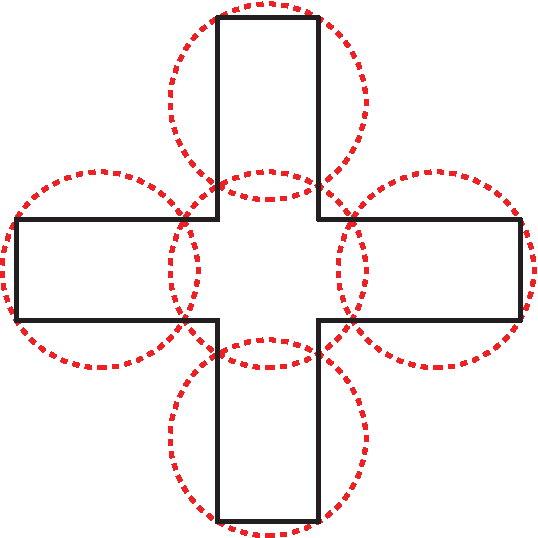
\includegraphics[scale=0.35]{chapters/osg/figures/exp_fig-e-eps-converted-to.pdf}
		\vspace*{1.5mm}
    \caption[An example showing an optimal solution of using five discs to cover the plus-shaped polygon]
    {An example showing an optimal solution of using five discs
		to cover the plus-shaped polygon. The solution is optimal for both 
		\opgt and \orgt formulations.}
    \label{fig:osg-example}
\end{figure}



\section{Intractability of Approximate Optimal Guarding of Simple Polygon}\label{sec:osg-complexity}
In this section, we prove that \osgt with the set being a simple polygon is 
strongly NP-hard to approximate within a factor of $\alpha = 1.152$, through 
a sequence of auxiliary NP-hardness results. 
%
First, in Section~\ref{subsec:3regular}, we prove an intermediate result 
that the vertex cover problem is NP-complete on planar bridgeless 
$3$-regular graphs.
% 
Next, in Section~\ref{complexity:3netcomp}, starting from a planar bridgeless 
$3$-regular graph, we construct a structure which we call {\em $3$-net} and 
prove the the problem of finding the minimum coverage radius of the 
$3$-net is NP-hard to approximate within $\alpha$. 
% 
Then, in Section~\ref{subsec:osgthard}, we apply a straightforward 
reduction to transform the $3$-net into a simple polygon to complete
the hard-to-approximate proof for \osgt for simple polygons.
%

We then further show the inapproximability of the special \opgt setup 
when each robot can only guard at most two disjoint perimeter segments 
(Section~\ref{subsec:2-seghard}), contrasting the FPTAS for the special 
\opgt setup when each robot can only guard a continuous perimeter 
segment in Section~\ref{subsec:singleseg}.

\subsection{Vertex Cover on Planar Bridgeless $3$-Regular Graph}\label{subsec:3regular}
Our reduction uses the hardness result on the vertex cover problem for planar 
graphs with maximum degree $3$ \cite{garey1977rectilinear}. Such a vertex cover 
problem can be fully specified with a 2-tuple $(G, k)$ where $G = (V, E)$ is a 
planar graph with max degree $3$ and $k$ is an integer specifying the allowed 
number of vertices in a vertex cover. We note that the result has been 
suggested implicitly in \cite{mohar2001face}; we provide an explicit account 
with a simple proof. 

\begin{lemma}
Vertex cover on planar bridgeless $3$-regular graph is NP-complete.
\end{lemma}
\begin{proof}
For a given planar graph $G$ with max degree $3$ and an integer $k$,
we construct a planar bridgeless $3$-regular graph $G''$ and provide an 
integer $k''$ such that $G$ has a vertex cover of size $k$ if and only 
if $G''$ has a vertex cover of size $k''$.

\begin{figure}[ht]
    \vspace*{2mm}
    \centering
    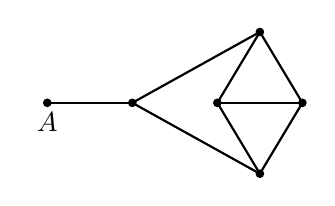
\begin{tikzpicture}[scale = .9]
        \draw[black, thick] (-0.8, 0) -- (-2,0);
        \draw[black, thick] (-0.8, 0) -- (1,1);
        \draw[black, thick] (0.4, 0) -- (1,1);
        \draw[black, thick] (1.6, 0) -- (1,1);
        \draw[black, thick] (-0.8, 0) -- (1,-1);
        \draw[black, thick] (0.4, 0) -- (1,-1);
        \draw[black, thick] (1.6, 0) -- (1,-1);
        \draw[black, thick] (0.4, 0) -- (1.6,0);
        \filldraw[black] (-0.8,0) circle (1.5pt);
        \filldraw[black] (0.4,0) circle (1.5pt);
        \filldraw[black] (1.6,0) circle (1.5pt);
        \filldraw[black] (-2,0) circle (1.5pt) node[anchor = north] {$A$};
        \filldraw[black] (1,-1) circle (1.5pt);
        \filldraw[black] (1,1) circle (1.5pt);
  			 %\node at (-2, 0) {\small{$A$}}; 
    \end{tikzpicture}
		\vspace*{2mm}
    \caption{A gadget that can be attached to a degree one or two vertices
		(at the point $A$) in a max degree $3$ graph to make all vertices have
		degree $3$. With each addition of the gadget, we increase the vertex 
		cover by a size of $3$, regardless of whether $A$ is part of a vertex 
		cover.}
    \label{fig:structure-hook}
\end{figure}

The reduction first makes $G$ $3$-regular by attaching (one or two of) the 
gadget shown in Fig.~\ref{fig:structure-hook} to $v \in G$ that are not 
degree $3$. This results in a $3$-regular graph $G'$. For each attached 
gadget, $k$ is bumped up by $3$, i.e., we let $k'$ for $G'$ be $k' = k 
+ 3(3|V(G)| - 2|E(G)|)$. It is straightforward to see that $G$ has a vertex 
cover size of $k$ if and only if $G'$ has a vertex cover size of $k'$.

\begin{figure}[!ht]
    \centering
    \raisebox{10mm}
    {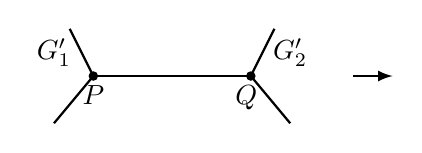
\begin{tikzpicture}
        \draw[black, thick] (-1,0) -- (1,0);
        \draw[black, thick] (-1,0) -- (-1.3,0.6);
        \draw[black, thick] (-1,0) -- (-1.5,-0.6);
        \draw[black, thick] (1,0) -- (1.3,0.6);
        \draw[black, thick] (1,0) -- (1.5,-0.6);
        \draw[black, thick, -latex] (2.3, 0) -> (2.8,0);
        \filldraw[black] (-1.5,0) node[anchor=south] {$G_1'$};
        \filldraw[black] (1.5,0) node[anchor=south] {$G_2'$};
        \filldraw[black] (-1,0) circle (1.5pt) node[anchor=north] {$P$};
        \filldraw[black] (1,0) circle (1.5pt) node[anchor=north] {$Q\,\,$};
    \end{tikzpicture}
    }
    \hfill
    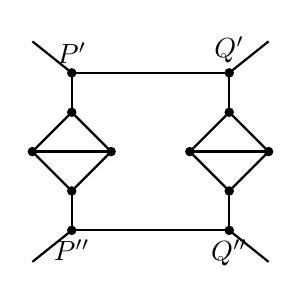
\begin{tikzpicture}
        \coordinate(p1) at (-1.5, 0);
        \coordinate(p2) at (-0.5, 0);
        \coordinate(p3) at (-1, 0.5);
        \coordinate(p4) at (-1, -0.5);
        
        \coordinate(p5) at (-1, 1);
        \coordinate(p6) at (-1, -1);
        
        \coordinate(p7) at (-1.5, 1.4);
        \coordinate(p8) at (-1.5, -1.4);

        \coordinate(q1) at (0.5, 0);
        \coordinate(q2) at (1.5, 0);
        \coordinate(q3) at (1, 0.5);
        \coordinate(q4) at (1, -0.5);

        \coordinate(q5) at (1, 1);
        \coordinate(q6) at (1, -1);
        \coordinate(q7) at (1.5, 1.4);
        \coordinate(q8) at (1.5, -1.4);
        
        \draw[black, thick] (p1) -- (p2);
        \draw[black, thick] (p1) -- (p3);
        \draw[black, thick] (p1) -- (p4);        
        \draw[black, thick] (p2) -- (p3);
        \draw[black, thick] (p2) -- (p4);
        \draw[black, thick] (p6) -- (p4);
        \draw[black, thick] (p5) -- (p3);
        

        \draw[black, thick] (q1) -- (q2);
        \draw[black, thick] (q1) -- (q3);
        \draw[black, thick] (q1) -- (q4);        
        \draw[black, thick] (q2) -- (q3);
        \draw[black, thick] (q2) -- (q4);
        
        \draw[black, thick] (q6) -- (q4);
        \draw[black, thick] (q5) -- (q3);
        
        \draw[black, thick] (q5) -- (p5);
        \draw[black, thick] (q6) -- (p6);
        
        \filldraw[black] (p1) circle (1.5pt);
        \filldraw[black] (p2) circle (1.5pt);
        \filldraw[black] (p3) circle (1.5pt);
        \filldraw[black] (p4) circle (1.5pt);
        \filldraw[black] (p5) circle (1.5pt) node[anchor=south] {$P'$};
        \filldraw[black] (p6) circle (1.5pt) node[anchor=north] {$P''$};
        
        \filldraw[black] (q1) circle (1.5pt);
        \filldraw[black] (q2) circle (1.5pt);
        \filldraw[black] (q3) circle (1.5pt);
        \filldraw[black] (q4) circle (1.5pt);
        \filldraw[black] (q5) circle (1.5pt) node[anchor=south] {$Q'$};
        \filldraw[black] (q6) circle (1.5pt) node[anchor=north] {$Q''$};
        
        \draw[black, thick] (p5) -- (p7);
        \draw[black, thick] (p6) -- (p8);
        \draw[black, thick] (q5) -- (q7);
        \draw[black, thick] (q6) -- (q8);
        
    \end{tikzpicture}
    \vspace{.5mm}
    \caption{Transformation that removes bridge $PQ$ and does not introduce new bridges.
    The minimum vertex cover number is increased by $6$ after each transformation.}
    \label{fig:rmbridge}
\end{figure}

In the second and last step, we remove bridges in $G'$. As in 
Fig.~\ref{fig:rmbridge}, for a bridge $PQ$ that divides $G'$ into $G_1'$ 
(containing $P$) and $G_2'$ (containing $Q$), we split the bridge edge 
$PQ$ using the illustrated transformation, which yields a new graph $G''$
that is planar, bridgeless, and $3$-regular, after all bridges are removed
this way. For each such augmentation, the size of the vertex cover is 
bumped up by six. Let $br(G')$ be the number of bridges in $G'$, $G'$ has 
a vertex cover of size  $k'$ if and only if $G''$ has a vertex cover 
of size $k'' = k'+6br(G')$. This completes the proof. 
\end{proof}


\subsection{Hardness on Optimally Guarding a $3$-Net}\label{complexity:3netcomp}
Starting from a planar cubic graph $G$, we construct a structure that we call 
$3$-net, $T_G$, as follows. 
%
First, similar to \cite{feder1988optimal}, to embed $G$ into the plane, 
an edge $uw \in E(G)$ is converted to an odd length path $uv_1, v_1v_2, 
\ldots, v_{2m}w$ where $m > 3$ is an integer. We note that $m$ is different
in general for different edges of $G$. 
%  to be decided later. 
Denote such a path as $u\cdots w$; each edge along $u\cdots w$ is straight 
and has unit edge length. We also require that each path is nearly straight 
locally. 
% This point will be made more precise later.
%
For a vertex of $G$ with degree $3$, e.g., a vertex $u \in V(G)$ 
neighboring $w, x, y \in V(G)$, we choose proper configurations and lengths for 
paths, $u\cdots w$, $u\cdots x$, and $u\cdots y$ such that
these paths meet at $u$ forming pairwise angles of $2\pi/3$. We denote the 
resulting graph as $G'$, which becomes the {\em backbone} of the 
$3$-net $T_G$. 

From here, a second modification is made which completes the 
construction of $T_G$. In each previously constructed 
path $u\cdots w = uv_1\ldots v_{2m}w$, for each $v_iv_{i+1}$, $1 \le i
\le 2m-1$, we add a line segment of length $\sqrt{3}$ that is 
perpendicular to $v_iv_{i+1}$ such that $v_iv_{i+1}$ and the line 
segment divide each other in the middle. A graphical illustration is
given in Fig.~\ref{fig:path-bar}. 
% We note that the bars do not need to be connected to the backbone $G'$. 
$G'$ and the bars form the 
$3$-net, which we denote as $T_G$. An example of transforming $K_4$
into a {\em 3-net} is given in Fig.~\ref{fig:3-net}.

\begin{figure}[ht]
% \vspace*{-4mm}
    \centering
		\vspace*{1mm}
    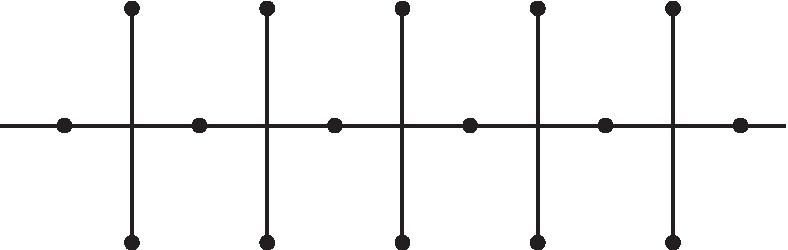
\includegraphics[scale=0.3]{chapters/osg/figures/edgepath-eps-converted-to.pdf}
		\vspace*{3mm}
% \vspace*{-4mm}
    \caption{Structure within the odd length path and attached 
		perpendicular ``bars'' with length $\sqrt{3}$. Regarding the 
		representation of such non-integral coordinates in the problem 
    input, 
    we may scale the coordinates to some certain extent and
    round them to integers so that the relative distance between
    each other is precise enough
    for the proof.
    % a precise enough fractional representation is enough 
    % for the proof due to the inapproximability gap in the result.
    }
		\vspace*{-1mm}
    \label{fig:path-bar}
\end{figure}

\begin{figure}[ht]
    \centering
    % \vspace*{-8mm}\
    \raisebox{14mm}{
    \begin{overpic}[scale=0.2]{chapters/osg/figures/k4-eps-converted-to.pdf}
      % \put(53,36){\color{black}$w$}
      \put(115,23){$\to$}
      \end{overpic}
    }
      \begin{overpic}[scale=0.4]{chapters/osg/figures/k4_after-eps-converted-to.pdf}
        \end{overpic}
    \caption{Illustration of a $3$-net obtained from $K_4$, the complete graph on 
		$4$ vertices.}
    % \caption{A $3$-net constructed over the backbone in Fig.~\ref{fig:backbone}.
        % \textcolor{red}{Siwei: update this to be based on $G'$ from Fig.~\ref{fig:backbone}}
        % }
    \label{fig:3-net}
\end{figure}

Let $L$ be the number of (unit length) edges of $G'$ (i.e., $L = 
\sum_{uv \in E(G)}len(u\cdots w)$). 
\begin{lemma}\label{l:bl}
A planar bridgeless $3$-regular graph $G$ has a vertex cover of size 
$k$ if and only if its transformed 3-net $T_G$ can be covered
by $K = k + (L-|E(G)|)/2$ circles of radius approximately $\alpha = 1.152$.
\end{lemma}
\begin{proof}
If $G$ has a vertex cover of size $k$, then we put $k$ circles of radius $1$
at the centers of the corresponding vertices in $T_G$. 
%
For each odd length path $u\cdots w$, since either $u$ or $w$ is already 
selected as the circle center, applying one coverage pattern shown
in Fig.~\ref{fig:pathcover} with $(len(u\cdots w) - 1)/2$ circles will cover 
the rest of $u\cdots w$ and all bars on it. So, the total number of circles
used is $K$ to cover all of $T_G$. 

\begin{figure}[!ht]
  \vspace*{0mm}
      \centering
      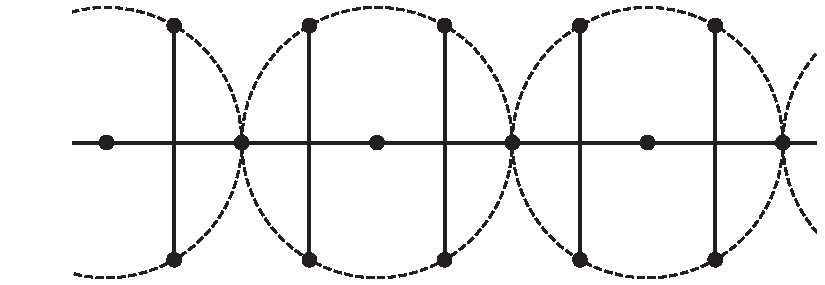
\includegraphics[scale=0.3]{chapters/osg/figures/edgepath1-eps-converted-to.pdf}\vspace{3mm}
      \hfill
      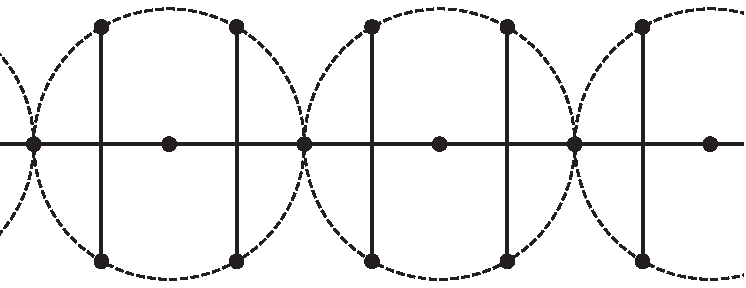
\includegraphics[scale=0.3]{chapters/osg/figures/edgepath2-eps-converted-to.pdf}
  \vspace*{0mm}
     \caption{Two coverage patterns on an odd length path with robots of 
      range sensing radius $1$ which is less than $\alpha$.}
      \label{fig:pathcover}
  \end{figure}
  
  \begin{figure}[!ht]
    \centering
    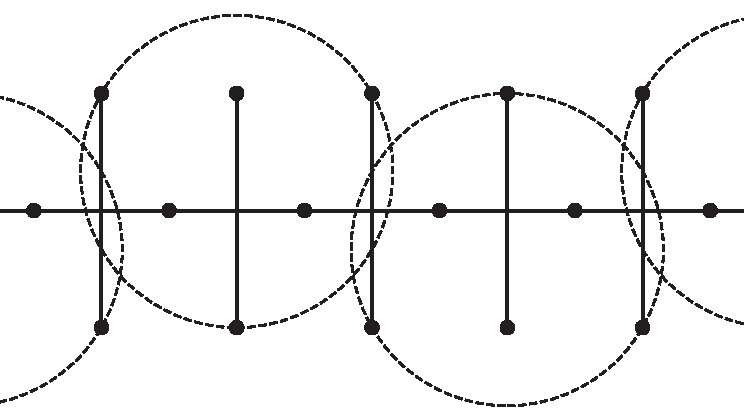
\includegraphics[scale=0.33]{chapters/osg/figures/edgepath3-eps-converted-to.pdf}
  \vspace*{1mm}
    \caption{Asymmetrical coverage of $4$ endpoints requiring a circle of 
    radius at least $2\sqrt{3}/3\approx 1.155$.}
    \label{fig:pathcovert}
  \end{figure}

The ``if'' part requires more analysis. Consider $T_G$ that can be covered 
by $K$ circles of radius $r \approx \alpha$. For a path $u\cdots w$ on $T_G$ whose 
length is $2m+1$, there are $2m-1$ vertical bars associated with it. Consider 
the $4m-2$ endpoints of these vertical bars. We note that (as shown in 
Fig.~\ref{fig:pathcovert}), it requires a radius of $2\sqrt{3}/3\approx 1.155$ 
for a circle to cover $4$ bar endpoints in an asymmetrical manner (three endpoints
on one side of the path, one on the other). Since 
we set the radius of coverage circle to be about $\alpha = 1.152$ (actually, 
between $1.152$ and $1.153$),
a circle may only cover up to $4$ bar endpoints. When a circle does cover $4$ 
bar endpoints, it must use a symmetrical coverage pattern, i.e. $4$ endpoints
on two bars, resulting in fully covering two bars. For the 
rest of the proof, we use ``circle'' to mean circles with a radius of $\alpha$,
unless otherwise stated explicitly. 

Since there are $4m - 2$ bar endpoints, it requires $m$ circles to cover all 
bar endpoints when $m \ge 3$. Moreover, at least one circle must cover $4$ 
bar endpoints by the pigeonhole principle. Fixate on such a circle $S$, which 
must have symmetric coverage, we examine the bars on one side of it, say the 
left side, assuming the path $u\cdots w$ is horizontal. If there are more 
than two bars to the left, then it is always beneficial to cover the two bars 
immediately to the left of $S$ using another circle. To see that this is the 
case, look at the two bars ($DE$ and $FH$) and the two associated unit 
length edges ($AB$ and $BC$) to the left of $S$ in Fig.~\ref{fig:two-bar}.
It can be computed that the circle $S$ to the right can cover a maximum 
length of $0.412$ of $AB$ to $A'$. Circles to the left of $S$ then must cover 
$A'B$. Let the circle covering $A'$ be $S'$. We may assume that 
$S'$ covers at least one of $D$ and $E$ (otherwise, at least one more circle 
$S''$ must be added that fall between $S'$ and $S$, in which case $S''$ 
must also cover $A'$). 

  \begin{figure}[ht]
  \vspace*{0mm}
    \centering
     \begin{overpic}[width=0.7\columnwidth]{chapters/osg/figures/two-bar-notext-eps-converted-to.pdf}
     \put(95, 31){$S$}
     \put(62.5,13){$A$}
     \put(50,22.5){$A'$}
     \put(44.3,13){$B$}
     \put(27,13){$C$}
     \put(57.5,36){$D$}
     \put(57.5,0){$E$}
     \put(41,32){$F$}
     \put(41,1.5){$H$}
     \put(14,26){$S'$}
     \end{overpic}
  \vspace*{3mm}
    \caption{When there are enough bars left, it is always better to cover
		two bars at a time with a circle. Two extremal cases of $S'$ covering
		$A'$ and $D$ but not $E$ are shown (as dashed circles), which amounts 
		to rotating the circle $S'$ around $D$.}
    \label{fig:two-bar}
  \end{figure}

If $S'$ covers $A'$ and only one of $D$ or $E$, say $D$, some other circle 
$S''$ must cover $E$. In this case, the coverage region of $S'$ and $S''$ are 
bounded by circles of radius approximately $2.304$ with center at $D$ and $E$, 
respectively. It is readily observed that $S'$ and $S''$ can reach at most one 
more bar to
the left of $FH$ (we note that $S'$ and $S''$ will not be able reach structures
on the $3$-net beyond $u\cdots w$ path). In this case, we can instead move $S'$ 
cover $A'C$, $DE$, and $FH$, and move $S''$ cover the bar to the left of $FH$ 
and potentially one more bar. Therefore, we may assume that $S'$ covers bar 
endpoints $D, E, F$, and $H$, symmetrically along the $u\cdots w$ path. 
Following the reasoning, we may assume that all bars on paths are covered, 
two at a time by a circle in a symmetrical manner, until there are one or two 
bars left before a path reaches a junction where it meets other paths. 

Because there are odd number of bars on a path, the symmetric coverage pattern 
extends until one side of a path has two bars remaining while the other side
has one bar. $m - 2$ circles have been used so far, which means that at least 
two more circles are needed to cover the remaining three bars. Without loss of 
generality, assume two bars out of these three are adjacent and are on the left 
end of $u\cdots w$ and one is on the right. Denote these bars as $b_1, b_2$, 
and $b_3$, from left to right. We call the end of a path with two bars the 
{\em even end} (e.g., the side ending with two bars $b_1$ and $b_2$) and the 
end of the path with one bar the {\em odd end} (e.g., the side ending with one 
bar $b_3$). 

We now examine the coverage of $b_2$ (see Fig.~\ref{fig:end-two-bar} where 
$b_1$ corresponds to $CD$ and $b_2$ corresponds to $AB$). Again, if the two 
endpoints $A$ and $B$ of $b_2$ are covered by more than one circle, then one 
of these two circles can be replaced with one that fully covers $b_1$ and 
$b_2$ (the solid circle in Fig.~\ref{fig:end-two-bar}), since a circle 
covering only one endpoint of $b_2$ (e.g., $B$) will not be able to reach 
structures outside $u\cdots w$. By now, $m-1$ circles have been used and to 
cover $u \cdots w$, at least two more circles are needed at the two ends 
(i.e., $m+ 1$ circles are required to cover $u\cdots w$). 

  \begin{figure}[ht]
    \centering
     \begin{overpic}[width=0.6\columnwidth]{chapters/osg/figures/end-two-bar-notext-eps-converted-to.pdf}
     \put(18, 28.5){$u$}
     \put(64.5, 43){$A$}
     \put(60, 10){$B$}
     \put(51, 39){$C$}
     \put(51, 15.5){$D$}
     \put(68,10){\rotatebox{-12}{{\small $r=2.304$}}}
		 \end{overpic}
  \vspace*{1mm}
    \caption{When there are two bars at the end of a path, it is preferred
		to cover them with a single circle (in red). The dotted circle shows that 
		a circle of radius $2*\alpha$ covering $B$ will not be able to reach 
		structures outside $u\cdots w$.}
    \label{fig:end-two-bar}
  \end{figure}


Next, instead of examining $b_3$, we examine the possible configurations at 
junctions where paths meet. There are four possible cases that contains 
$0$-$3$ odd ends. For the case where only even ends meet, one additional 
circle is needed to cover the rest of the junction 
(Fig.~\ref{fig:junction}(a)). When there is one odd end and two even ends 
(Fig.~\ref{fig:junction}(b)), it requires one more circle to cover the 
junction. This constraint is how the radius $\alpha = 1.152$ is obtained 
(more precisely, with circles with radius 1.153, no additional circles are 
needed at the junction). When there are two odd ends and one even end 
(Fig.~\ref{fig:junction}(c)), at least one more circle is needed to cover 
the the junction. For the last case (Fig.~\ref{fig:junction}(d)), no 
additional circles are needed. The cases where additional cycles are needed 
correspond to the junction vertex being selected as a vertex cover. 
It is straightforward to observe that the constructed vertex cover is a valid 
one. The cover has size of $K-(L-|E(G)|)/2$. 

\begin{figure}[!ht]
	\vspace*{4mm}
  \centering
  \hspace{-10mm}
\begin{overpic}[scale=0.66]{chapters/osg/figures/junction-eps-converted-to.pdf}
  \put(16, 0){(a)}
  \put(40, 0){(b)}
  \put(64, 0){(c)}
  \put(88, 0){(d)}
\end{overpic}
\vspace*{2mm}
  \caption{The four possible patterns at the junction using circles of radius 
	less than $\alpha = 1.152$. When we increase the radius to $r = 1.152259$, 
	circles shown in (b) and (c) can successfully cover the junction and the odd 
	ends.}
  \label{fig:junction}
\end{figure}
\end{proof}

It is clear that Lemma~\ref{l:bl} holds for discs with radius in 
$[1, \alpha)$. Thus, approximating $size(T_G, K)$ to less than a 
factor of $\alpha$ will decide whether $G$ has a vertex cover of 
$k$, yielding the hard-to-approximate result.
Also, it can be observed that all lengths are polynomial with respect to 
the problem input size, which implies strongly NP-hardness.
\begin{theorem}\label{t:3nethard}
The minimum radius for cover a $3$-net using 
% $(({L-|E|})/{2}+k)$ 
$k$ circular discs 
% while minimizing the maximum disc radius 
is strongly NP-hard to approximate within a 
factor of $\alpha = 1.152$.
\end{theorem}


\subsection{From $3$-Nets to Simple Polygons}\label{subsec:osgthard}
We proceed to show that \osgt is hard to approximate for a simply polygon 
by converting a $3$-net into one. Along the backbone $G'$ of a $3$-net 
$T_G$, we first expand the line segments by $\delta$ to get a 2D region  
(see Fig.~\ref{fig:door}(a)). We may describe the interior of the resulting 
polygon as 
\vspace*{-1mm}
\[P=\{p\in \R^2\ |\ \min_{q\in T_G}(\lVert p-q\rVert_1)\leq \delta/2\}\]
\vspace*{-4mm}

For small enough $\delta$, it's clear that $P$ is a polygon with holes.
Let $K = (({L-|E|}){2}+k)$, it holds that
\vspace*{-1mm}
\begin{align*}
&size(K, T_G) \leq               size(K, P)\leq size(K, T_G) + \delta,\\
&size(K, T_G) \leq      size(K, \partial P)\leq size(K, T_G) + \delta.
\end{align*}
\vspace*{-5mm}

To convert the structure into a simple polygon, we can open ``doors'' of 
width $\delta$ on the structure to get rid of the holes (see 
Fig.~\ref{fig:door}(b)). Each opening removes one hole from $P$. This is 
straightforward to check; we omit the details. 
\begin{figure}[ht]
		\centering
		\vspace*{0mm}
    \begin{small}
    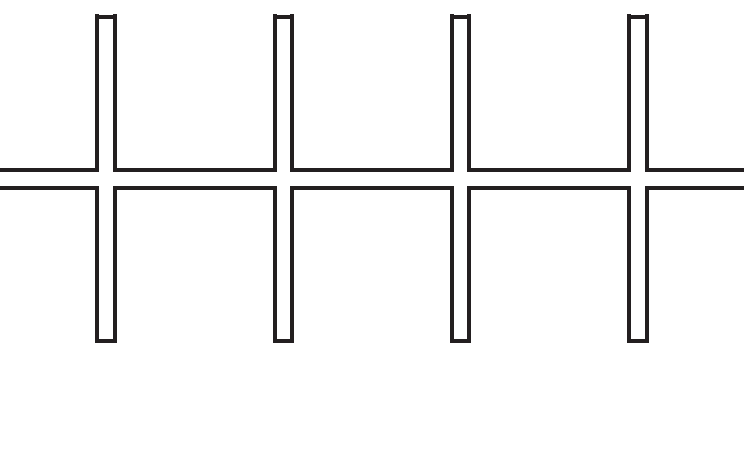
\includegraphics[scale=.3]{chapters/osg/figures/holes-eps-converted-to.pdf} 
    \hfill
    \begin{overpic}[scale=.3]{chapters/osg/figures/doors-eps-converted-to.pdf}
        \put(50,42){$\delta$}
        \put(-75,3){(a)}
        \put(46,3){(b)}
    \end{overpic}
	  \end{small}
		\vspace*{1mm}
    \caption{(a) A $3$-net $T_G$ maybe readily converted into a simple polygon 
		$P$ with holes by expanding along its backbone. (b) Creating a ``door'' 
		of width $\delta$ will remove one hole from $P$.}
    \label{fig:door}
\end{figure}

Denoting the resulting simple polygon as $P'$, we have
\vspace*{-1mm}
\begin{align*}
&size(K, P) - \delta  \leq               size(K, P')\leq size(K, P),\\
&size(K, \partial P) - \delta  \leq      size(K, \partial P')\leq size(K, \partial P).
\end{align*}
\vspace*{-5mm}

Therefore, both $size(k, P')$ and $size(k, \partial P')$ are between 
$size(k, T_G) - \delta$ and $size(k, T_G) + \delta$. Suppose the \osgt for 
$\partial P'$ or $P'$ has a polynomial approximation algorithm with 
approximation ratio $1.152 - \varepsilon$ where $\varepsilon > 0$, let $\delta = 
\varepsilon/2$, then the optimal guarding problem for the $T_G$ can 
be approximated within 1.152 disobeying the inapproximability gap by 
Theorem~\ref{t:3nethard}. Therefore,

\begin{theorem}\label{t:osgthard}
\osgt is NP-hard and does not admit a polynomial time approximation 
within a factor of $\alpha$ with $\alpha = 1.152$, unless 
P$=$NP.
\end{theorem}

\subsection{\opgt with Sensor Guarding Restrictions}\label{subsec:2-seghard}
The inapproximability gap from Theorem~\ref{t:osgthard} prompts us to 
further consider restrictions on the setup with the hope that meaningful 
yet more tractable problems may arise. On natural restriction is to 
limit the number of continuous segments a mobile sensor may cover. As 
will be shown in Section~\ref{subsec:singleseg}, if a mobile sensor may 
only guard a single continuous perimeter segment, a 
$(1 + \varepsilon)$-optimal solution can be computed efficiently. 
On the other hand, it turns out that if a sensor can guard up to two 
continuous perimeter segments, \opgt remains hard to approximate. 

\begin{theorem}\label{them:twoconthard}
\opgt of a simple polygon cannot be approximated within $\alpha\approx 1.152$ 
even when each robot can guard no more than two continuous boundary segments,
unless P$=$NP.
\end{theorem}
\begin{proof}
Due to \cite{petersen1891}, every bridgeless $3$-regular graph $G$ has a 
perfect matching. We can obtain such a perfect matching of the $3$-regular 
graph using Edmonds' Blossom algorithm in polynomial time\cite{edmonds_1965}. 
Doubling the edges in the perfect matching, we can then obtain a 4-regular 
graph $G'$. 

\begin{figure}[ht]
		\vspace*{-2mm}
    \centering
    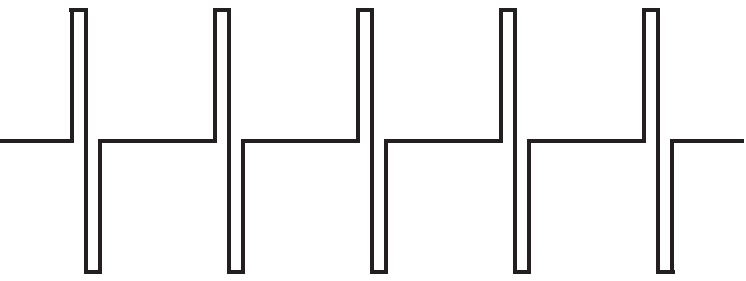
\includegraphics[scale=0.3]{chapters/osg/figures/1going-eps-converted-to.pdf}\hspace{2mm}
	  \begin{overpic}[scale=.3]{chapters/osg/figures/2going-eps-converted-to.pdf}
        \put(-55,-10){(a)}
        \put(49,-10){(b)}
    \end{overpic}
		\vspace*{6mm}
    \caption{(a) Part of the augmented Eulerian path for non-doubled 
		paths. (b) Part of the augmented Eulerian path for doubled paths.}
    \label{fig:path_exp}
		\vspace*{-1mm}
\end{figure}

The Eulerian tour on $T_G$ may have self-intersections, which 
will prevent the tour from being a simple polygon. To address this, we may use 
one of two possible solutions outlined in Fig.~\ref{fig:eliminter} to eliminate
the self-intersections. 
\begin{figure}[ht]
    		\vspace*{2mm}
				\centering
	  \begin{overpic}[width=\columnwidth]{chapters/osg/figures/t345-eps-converted-to.pdf}
        \put(12,-6){(a)}
        \put(48,-6){(b)}
        \put(84,-6){(c)}
    \end{overpic}
		\vspace*{3mm}
        \caption{In order to eliminate possible self-intersections in 
				(a), we may transform it into one of the solutions given in 
				(b) and (c) to make the Eulerian tour remain connected (one 
				of the two solutions will satisfy this).}
        \label{fig:eliminter}
\end{figure}

At this point, we readily observe that Theorem~\ref{t:osgthard} applies. 
Furthermore, an optimal solution always allows each mobile sensor to 
cover only two continuous perimeter segments. This is clear in the middle 
of any paths of $T_G$; at junctions, the polygon boundary will be either 
one of two possibilities shown in Fig.~\ref{fig:2types}, where a sensor
again covers at most two continuous segments of the simple polygon. 
\begin{figure}[!ht]
    \centering
    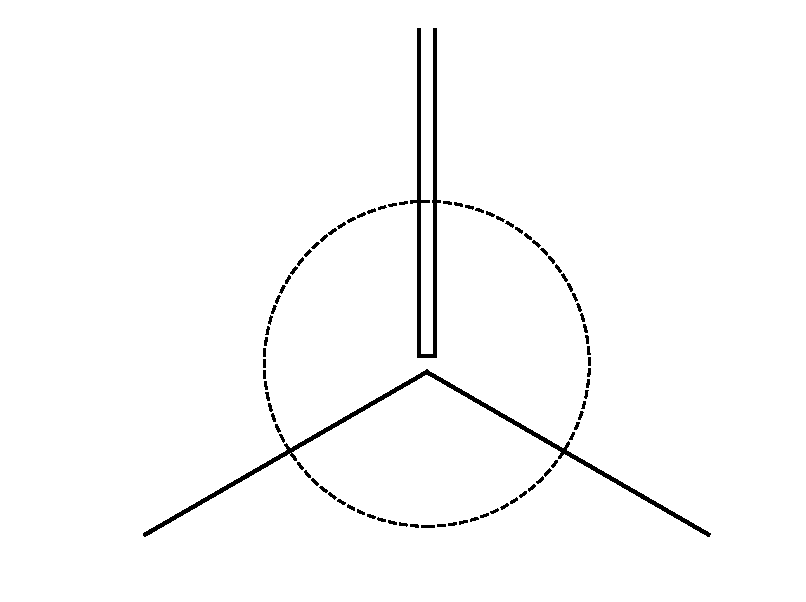
\includegraphics[scale=.29]{chapters/osg/figures/t1-eps-converted-to.pdf}
    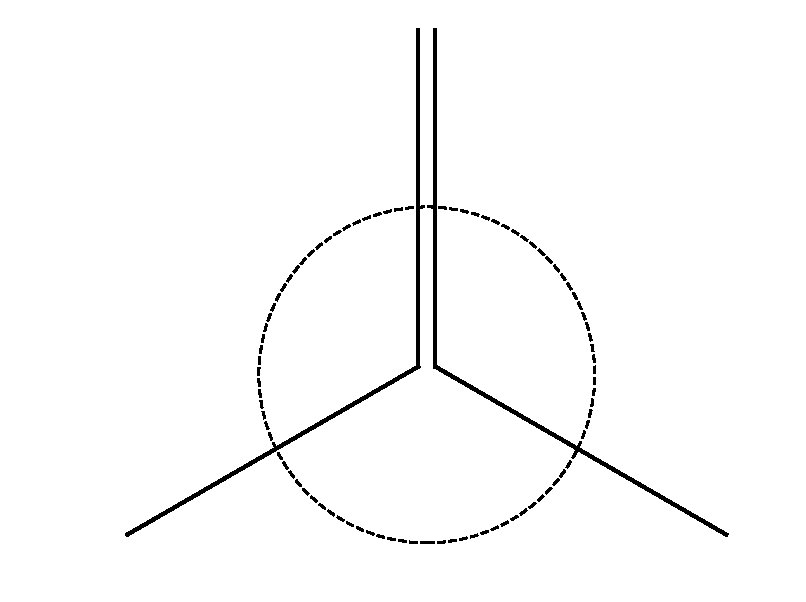
\includegraphics[scale=.29]{chapters/osg/figures/t2-eps-converted-to.pdf}
    \caption{The figure shows two possible types of boundaries near a 
		vertex with degree of $4$. A robot near the vertex will only be able 
		to cover two disjoint but individually continuous boundary segments 
		with sensing radius less than $\alpha$ if the solution is to be optimal.}
    \label{fig:2types}
\end{figure}
\end{proof}


\section{Effective Algorithmic Solutions for \osgt}\label{sec:osg-algo}
\def\algomed{\textsc{Min\_Enclose\_Disc}\xspace}
In this section, we present several algorithmic solutions for \osgt. 
First, a fully polynomial approximation scheme (FPTAS)
is presented that solve \opgt with the additional requirement 
that each sensor is responsible for a continuous perimeter segment. 
This contrasts Theorem~\ref{them:twoconthard}. Then, we show that 
there exist polynomial time algorithms that readily guarantee a
$(2+\varepsilon)$-approximation for \osgt. This is followed by an 
integer linear programming (ILP) method that delivers high-quality
solutions (as compared with the $(2 + \varepsilon)$-approximate one)
and has good scalability. 

In preparation for introducing the result, we first describe a method
that is used for discretizing the problem. For a simple polygon $P$, 
we can approximately represent its boundary $\partial P$ as a set of 
balls with radius $\varepsilon$ along $\partial P$, by splitting  
$\partial P$ into $N=\lceil{len(\partial P)}/({2\varepsilon})\rceil$ 
continuous pieces of length at most $2\varepsilon$ and putting the balls' 
centers at their midpoints. 
%
Denote set of $\varepsilon$-balls as $S_B$, and the set of their centers 
as $S_O=\{o_1,\dots, o_N\}$. Since it holds that $size(k,\partial P) \leq 
size(k, S_B) \leq size(k, S_O) + \varepsilon \leq size(k, \partial P) 
+ \varepsilon$, the minimum coverage radius of the discritized version 
of covering $S_O$ will differ no more than $\varepsilon$ from the original 
problem of covering $\partial P$. Similarly, for covering the interior 
of $P$, we can put $P$ into a grid with cell side length $\varepsilon$, 
and set the center of the grid cells intersecting with $P$ as $S_O$, 
creating at most $N=O(({len(\partial P)}/{\varepsilon})^2)$ samples. 
The discretization process converts guarding $P$ or $\partial P$ to 
guarding $S_O$. 

\subsection{\opgt with Single Segment Guarding Limitation}\label{subsec:singleseg}
By Theorem.~\ref{them:twoconthard}, if a mobile sensor can guard up to two 
continuous perimeter segments, \osgt is hard to approximate within 
$1.152$-optimal. 
Translating this into guarding elements of $S_O$, this means that a sensor
can guard two {\em chains} of elements from $S_O$, where each chain contains 
some $m$ elements $o_1, \ldots, o_m$ that are neighbors along $\partial P$. 
Interestingly, if each sensor may only guard a single chain of elements 
from $S_O$, we may compute an optimal cover for $S_O$ using $O(N^2 \log N)$ 
time. This readily turns into a fully polynomial time approximation scheme 
(FPTAS) for \opgt. 
% based on efficent implementation of the expected linear time 
% implementation to get the Minimum Enclosing Disc of a set of points \cite{welzl1991smallest}\cite{Mark1997computation}.  
The algorithm operates by checking multiple times whether a given radius 
$r$ is sufficient for $k$ discs of the given radius to cover elements of 
$S_O$ where each disc covers only a single chain of elements. 

A single feasibility check is outlined in Algorithm~\ref{algo:cont}.
In the pseudo code, it is assumed that the indices are modulo $N$, e.g. 
$M[N+1] = M[1]$, $o_{N+1} = o_1$. 
%
Algorithm~\ref{algo:cont} is based on an efficient implementation of 
a subroutine \algomed (from e.g., \cite{welzl1991smallest,
Mark1997computation}) that computes the disc with minimum radius to 
enclose a given set of points in expected linear time. With this, a sliding 
window can be applied to find the rightmost $end$ for each $1\leq i\leq 
N$ such that $o_i, \dots, o_{end}$ can be enclosed in a circle of radius 
$r$. The length of this sequence is stored in $M[i]$. 

As $o_{end}$ cannot come around and meet $o_i$, the total call to 
\algomed is no more than $2N$. After this, the algorithm simply tries to put 
discs from each $o_i$ to cover as many centers as possible to see 
whether $S_O$ can be enclosed with $k$ discs. An optimization can be made 
by only examining starting point as $o_1, \dots, o_{M[1]+1}$, since there 
is no circle of radius of $r$ that can cover them together by the 
definition of $M$.
%
The apparent complexity of Algorithm~\ref{algo:cont} is $O(N^2)$. Since 
there are a total of $N$ points and $k$ robots, in a majority 
of cases a circle would enclose about $N/k$ points, which effectively 
lowers the time complexity to $O(N^2/k)$.

\def\algoptfeasi{\textsc{Opg\_2D\_Cont\_Feasible}}
\SetKw{Continue}{continue}
\SetKw{True}{true}
\SetKw{False}{false}
\begin{algorithm}
\begin{small}
\DontPrintSemicolon
\SetKwComment{Comment}{\%}{}
\caption{\textsc{Opg\_2D\_Cont\_Feasible}}    %($P$, $k$, $r$, $\varepsilon$)}}
\label{algo:cont}
\SetKwInOut{Input}{Input}
\SetKwInOut{Output}{Output}
\KwData{$S_O=\{o_1, \dots, o_N\}$, sample points in circular order\\
\qquad\quad$k$, the number of robots\\
\qquad\quad $r$, the candidate sensing radius}
\KwResult{\True or \False, indicating whether $S_O$ can be covered with k discs with radius $r$}
\vspace{2mm}

\If{{\sc Min\_Enclose\_Disc}($o_1, \dots, o_N$)$\leq r$} {\Return{\True}}
\vspace{1.5mm}

\Comment{\small Phase 1: find the maximum number of consecutive points a disc of radius $r$ can enclose
from each $c_i$.}%$arr[i]$ \small stores the number of continuous points the disc can enclose from $c_i$.}
\vspace{1.5mm}

$M\leftarrow$ an array of length $N$; $end\leftarrow 1$;\;
\vspace{1.5mm}

\For{$i=1$ \KwTo N}{
\While{{\sc Min\_Enclose\_Disc($o_i, \dots, o_{end+1}$) $\leq r$ }}{
    $end\leftarrow end+1$;\;
}
$M[i]\leftarrow end - i + 1$;\;
}
\vspace{1.5mm}

\Comment{\small Phase 2: try to tile from each $o_i$.}
\vspace{1.5mm}

\For{$i=1$ \KwTo $N$}{
$j \leftarrow i$, \quad $cnt \leftarrow k$;\;
\While{$cnt > 0$}{
    $j \leftarrow j + M[j]$;\;
    \If{$j-i \geq N$}{\Return{\True}}
    $cnt\leftarrow cnt-1$\;
}
}
\Return{\False}
\end{small}
\end{algorithm}



Note that for the optimal coverage radius $r^*$, it holds that $r_{min} = 
0 < r^* \leq {len(\partial P)}/({2k}) = r_{max}$. 
Recall that $N=\lceil len(\partial P)/(2\varepsilon)\rceil$.
Hence, after at most 
\[
  \log\frac{r_{max} - r_{min}}{\varepsilon} = \log(\frac{len(\partial P)}{2k\varepsilon})  = O(\log\frac{N}{k} )
\]
times of binary search on the optimal radius $r^*$ by calling \algoptfeasi, 
the search range of $r^*$ or the gap between $r_{max}$ and $r_{min}$ will 
be reduced to within $\varepsilon$. So, it takes expected $O(N^2 \log (N/k))$ 
time in total to get an approximate solution with radius at most $\varepsilon$ 
more than $size(k, S_O)$ or $size(k, \partial P)$.
\begin{theorem}\label{t:opgtsseg}
    Under the rule of continuous coverage, \opgt for a simple 
		polygon can be approximated to $(1 + \varepsilon)$-optimal in expected 
		$O(N^2\log N)$ time, and $O(({N^2}/{k} )\log(N/k))$ in most cases,
    where $N=\lceil{len(\partial P)}/({2\varepsilon})\rceil$.
\end{theorem}

\remark{In the running time complexity analysis, we implicitly 
used the assumption that $len(\partial P)$ is polynomial to problem input 
size (see Section~\ref{sec:problem}). Also, the algorithm given above
computes an $OPT + \varepsilon$ optimal solution. However, 
% due to the 
it can be naturally assumed that the optimal
sensing radius $OPT$ is lower bounded in realistic scenarios. 
So, an $(OPT + \varepsilon)$ solution
directly translates into a $(1 + \varepsilon)$-optimal solution. 
Lastly, using techniques similar to those from \cite{fenghangaoyu2019efficient,fengyu2020RAL}, 
we mention that results in this subsection readily extends to multiple 
simple polygons with gaps along the boundary. 
These arguments continue to apply throughout the rest of  
this section. 
%

Regarding the choice in implementation, the minimum enclosing disc problem 
(1-center problem) also has deterministic solution 
\cite{megiddo1983linear} in linear time, but a randomized algorithm is considered to be 
more efficient\cite{welzl1991smallest} and easier to implement.}

\subsection{$(2 + \varepsilon)$ Approximation}
In dealing with Euclidean $k$-clustering problems, two seminal methods 
are often brought out, both of which compute $2$-approximation solutions
for $k$-center problem in polynomial time. This is fairly close to the 
inapproximability gap of $1.822$ for Euclidean $k$-center
problem\cite{feder1988optimal}. The first 
\cite{hochbaum1985best, vazirani2013approximation} transforms the 
clustering problem to a dominating set problem and then applies parametric 
search on the cluster size (radius), resulting in a $2$-approximation in 
time $O(n^2\log n)$ with $n$ being the number of points to cover. 
A second method \cite{gonzalez1985clustering} takes 
a simpler farthest clustering approach by iteratively choosing the 
furthest point from the current centers as the new center. The method runs 
in $O(nk)$ but is subsequently improved to $O(n\log k)$ in 
\cite{feder1988optimal}. So, by applying either of them on $S_O$, we have

\begin{proposition}
    \osgt can be approximated to $(2 +\varepsilon)$-optimal in polynomial time 
		with $N=O({len(\partial P)}/{\varepsilon})$ samples for perimeter 
		guarding and $N=O(({len(\partial P)}/{\varepsilon})^2)$ samples for
    region guarding.
\end{proposition}

For evaluation, we implemented the farthest clustering approach 
\cite{gonzalez1985clustering}.

\subsection{Grid and Integer Programming-based Algorithm}
Approximation using grids \cite{har2011geometric} often exhibits good 
optimality guarantees and bounded time complexity. Seeing that and knowing
that \osgt is hard in general, we attempted grid-based integer linear programming 
(ILP) methods for solving \osgt with good success. Our ILP model 
construction is done as follows. 

%Grid-based representation
%and approximation, suprisingly, achieve close to optimal solution quality guarentee 
%as well as computational efficiency with nowadays mathematical programming libraries as 
%Gurobi\cite{optimization2019gurobi} or CPLEX \cite{cplex2009v12} etc.

Consider bounding the polygon $P$ of interest by an $m\times n$ square grid 
where each cell is $\varepsilon \times \varepsilon$, and denote $g_{ij}$ as the center 
of the cell at row $i$ and column $j$. If we limit the possible locations of 
each robot to the center of some grid cell, the optimal radius with this 
limitation will only be at most $\sqrt{2}\,\varepsilon / 2$ away from 
$size(k, S_O)$. This could be seen by moving the robot locations in the optimal deployment
to their nearest grid centers respectively and applying triangle inequality.

So, given a candidate radius $r$, to check the feasibility of whether 
$\partial P$ can be covered by $k$ circles of radius $r$, we adapt an 
approach for solving the $k$-center problem\cite{daskin2000new} with 
integer linear programming. Specifically, we create $m\times n$ boolean 
variables $y_{ij}$, $1\leq i\leq m$, $1\leq j \leq n$, indicating whether 
there is a robot at $g_{ij}$, then start to check the feasibility of 
following integer programming model.
\begin{align}
    \sum_{ 1\leq i\leq m }\,\sum_{1\leq j \leq n} y_{ij} \leq k\qquad \qquad \qquad \\
    \sum_{i,\ j\ s.t.\ \lVert g_{ij} - o_\ell\rVert_2\ \leq\ r} y_{ij} \geq 1 \text{ for each }\, 1\leq \ell \leq N\\
    y_{ij} \in \{0,1\}\ \qquad 1\leq i\leq m,\ 1\leq j \leq n
\end{align}
The first constraint says the number of locations is no more than $k$, and 
the second ensures each $o_\ell$ can be covered by at least one circle 
with radius $r$ illustrated in ~\ref{fig:ilpexample}.

\begin{figure}[!ht]
    \centering
		\vspace*{1mm}
		\begin{overpic}[width=1\columnwidth]{chapters/osg/figures/ilp_example-eps-converted-to.pdf}
        \linethickness{0.4mm}
        \put(40.2,25.3){\color{red}\vector(0.8,1.05){15.6}}
        \put(40.2,17){\color{red}\vector(1.45,-1.1){15.5}}
        \put(40,19){\color{blue}$o_{67}$}
        \put(69,24){\color{blue}$o_{67}$}
    \end{overpic}
		\vspace*{1mm}
    \caption{This perimeter guarding example illustrates constraint 
		($2$) for $o_{67}$ with $r=7$. The black dots are the sampled $S_O = 
		\{o_1, \dots, o_{100}\}$. In order to cover $o_{67}$, at least one 
		among the red color grid cell centers need to be selected as robot location.}
    \label{fig:ilpexample}
\end{figure}


When the ILP model has a feasible solution, $r^* = size(k, S_O) \leq r$ 
and $r\leq r^* = size(k, S_O) $ otherwise. This means that we can do a binary 
search on $r^*$, from an initial range of $r^* = size(k, S_O)$: $r_{min}^i=0 
<  r^* \leq {len(\partial P)}/({2k})=r_{max}^i$, until finally $r^f_{max} - 
r^f_{min}$ is reduced to the selected granularity of $\varepsilon$.

\begin{remark}
    With minor modifications, the ILP model applies to 2D region 
		guarding, where the number of constraint $(2)$ will then be $O(mn)$ 
		with one for each grid that intersects with the polygon in an $m\times n$ 
		grid. The initial upper bound set as $r^*$ be $len(\partial P)$ and 
		lower bound set as $\sqrt{{area(P)}/({k\pi})}$. It is also possible to 
		apply the $(2+\varepsilon)$-approximation algorithm and set the result 
		as the initial upper bound with the half of it as the initial lower 
		bound.
\end{remark}


\section{Evaluation and Application Scenarios}\label{sec:osg-expr}
For the three algorithms described in Section~\ref{sec:osg-algo}, we developed
implementations in C++ and evaluated them on an Intel Core i7 PC with a 
boost clock of 4.2GHz and 16GiB RAM. For solving ILP models, 
Gurobi solver \cite{optimization2019gurobi} is used. 
%
To evaluate the algorithms, we first generate a set of performance 
benchmarks obtained by subjecting these algorithms through a large set 
of benchmark cases. 
%
Following the synthetic benchmarks, we applied the algorithms on two 
potential application scenarios: guarding the outer perimeter of the 
Warwick Castle and monitoring a building for potential fire eruption 
points.
 
\subsection{Performance Benchmarks}
For creating synthetic benchmarks, to generate the test set $\W$, we 
created simple polygons with the number of vertices ranging between 
$10$ and $200$. 
%
For each instance of the tested polygon, vertices are picked uniform at 
random from $[0,1]\times[0,1]$ and the TSP tour among these vertices are 
used for generating a simple polygon of a reasonable shape.
%
An example is given in ~\ref{fig:osg-ilpexample}.

\def\opgtc{\textsc{Al\_OPG\_2D\_Cont}\xspace}
\def\opgtilp{\textsc{Al\_OPG\_2D\_ILP}\xspace}
\def\orgtilp{\textsc{Al\_ORG\_2D\_ILP}\xspace}
We first evaluate the computational performance of the special \opgt
algorithm where each sensor may cover a single continuous perimeter
segment; denote this algorithm as \opgtc.
%
Table~\ref{tab:osg-opgcont} lists the running time in seconds for 
various $N$ (number of discretized samples) and $k$ (number of guards). 
Various values of $N$ suggest the choices of $\varepsilon$ according to 
the setup of $N$ in Section~\ref{sec:osg-algo}, in this case 
$N=\lceil {len(\partial P)}/{(2\varepsilon)} \rceil$.
Each data point is an average of $100$ examples. As we can observe, the 
method has very good scalability. It also demonstrates the behavior that 
running time is inverse proportional to the number of guards, 
conforming with the statement about time complexity in Section~\ref{subsec:osg-singleseg}. 
% This is due to the larger range of sensing radius that must be searched. In 
% practice, sensing radius is often lower and upper bounded, which means 
% that the algorithm will generally perform better. 
The normalized 
average standard deviation is about $0.06$, which is pretty small. 

\begin{table}[!htbp]
    % \resizebox{1}{1}
    \centering
    \begin{small}
        \begin{tabularx}{0.49\textwidth}{|X|c|c|c|c|c|c|} 
        \hline
        \diagbox{\hspace{1.4mm}$N$\hspace{0.3mm}}{$k$\hspace{0.7mm}} & $5$ & $10$ & $20$ & $30$ & $50$ & $100$ \\
        \hline
        \hspace{5mm}500&0.097 &        0.044 &        0.019 &        0.013 &        0.007 &        0.004 \\
        \hline
        \hspace{5mm}800&0.257 &       0.118 &       0.054 &        0.036 &        0.019 &        0.011 \\
        \hline
        \hspace{4mm}1000&0.385 &       0.183 &       0.082 &        0.055 &        0.029 &        0.016 \\
        \hline
        \hspace{4mm}1500&0.912 &       0.436 &       0.203 &       0.120 &       0.073 &        0.039 \\
        \hline
        \hspace{4mm}2000&1.597 &      0.743 &       0.345 &       0.225 &       0.123 &       0.062 \\
        \hline        
        \end{tabularx}
    \end{small}
    \vspace{0.1in}
    \caption{
        Running time (seconds) for \opgtc.
    }
    \label{tab:osg-opgcont}
\vspace*{-1mm}
\end{table}


Since the $(2 + \varepsilon)$-optimal algorithm is extremely efficient, 
we do not report its running time. For the ILP methods, Table~\ref{tab:osg-opgilp}
and Table~\ref{tab:osg-orgilp} provide the running times for solving \opgt
\begin{table}[htbp]
    % \resizebox{1}{1}
    \centering
    \small{
        \begin{tabularx}{0.49\textwidth}{|X|c|c|c|c|c|c|} 
        \hline
        \diagbox{$GS$}{$k$} & $10$ & $15$ & $20$ & $30$ & $50$ & $100$ \\
        \hline
        \hspace{2.2mm}$50\times 50$   &0.219  &0.127  &0.092  &0.051  &0.023  &0.009\\
        \hline
        \hspace{1mm}$100\times 100$ &0.686  &0.383  &0.250  &0.141  &0.089  &0.033 \\ 
        \hline
        \hspace{1mm}$200\times 200$ &1.915         &1.132         &0.792  &0.444  &0.281  &0.115  \\
        \hline
        \hspace{1mm}$300\times 300$ &7.782         &4.201         &2.613         &1.513         &0.814  &0.435 \\
        \hline
        \hspace{1mm}$400\times 400$ &21.23        &11.63        &7.275         &3.827         &2.231         &1.318 \\        \hline
    \end{tabularx}
    }
    \vspace{0.1in}
    \caption{
        Running time (seconds) for \opgtilp.
    }
    \label{tab:osg-opgilp}
\end{table}
and \orgt, respectively (for convenience, denote these two methods as
\opgtilp and \orgtilp).
Each data point is an average over $10$ cases. 
$GS$ denotes the discrete grid size, suggesting the choice of the grid granularity $\varepsilon$
and the single grid cell size $\varepsilon \times \varepsilon$.
We observe that the ILP method is 
highly effective for solving \opgt and fairly good for solving \orgt. 
The normalized average standard deviation is about $0.125$ for \opgtilp
(which is reasonable) and $0.545$ for \orgtilp (which is relatively large). 

\begin{table}[htbp]
    % \resizebox{1}{1}
    \centering
    \small{
        \begin{tabularx}{0.49\textwidth}{|X|c|c|c|c|c|c|c|} 
        \hline
        \diagbox{$GS$}{$k$} &$10$ & $15$ & $20$ & $30$ & $50$ & $100$ \\
        \hline
        \hspace{2mm}$20\times 20$ &0.252  &0.245  &0.200  &0.170  &0.136  &0.094 \\\hline
        \hspace{2mm}$30\times 30$&1.413 &1.064 &0.886  &0.799  &0.858  &0.576 \\\hline
        \hspace{2mm}$40\times 40$&5.048 &3.598 &3.055 &2.252 &6.114 &1.156 \\\hline
        \hspace{2mm}$50\times 50$ &7.003 &5.617 &4.984 &5.836 &10.91 &0.925\\\hline
        \hspace{2mm}$80\times 80$ &87.14  &84.18   &82.09   &423.5 & $>$2e3 & $>$2e3 \\\hline
        \end{tabularx}
    }
    \vspace{0.1in}
    \caption{
        Running time (seconds) for \orgtilp.
    }
    \label{tab:osg-orgilp}
\end{table}

For solution quality, we compare \opgtc, \opgtilp,
and \orgtilp with the $(2 + \varepsilon)$-optimal solution. For example,
given a test case, let the resulting radius for \opgtc be $r_1$ 
and that for
the $(2+\varepsilon)$-optimal algorithm be $r_2$, we compute the optimality
gain as the reduce of coverage radius over $r_2$ in percentage, 
that is $(r_2 - r_1)/r_2 \cdot 100$. These are then averaged over $10$ cases.
Selected representative results (only three out of a total of 18 rows) are 
given in Table~\ref{tab:osg-comp}. 
In the table, m denotes the method where $\mathbf{1} = $ \opgtc, $\mathbf{2} =$ \opgtilp, 
and $\mathbf{3} = $\orgtilp. Number of samples for \opgtc is set to $2000$. Grid
size for \opgtilp is $200\times 200$. Grid size for \orgtilp is set 
to $40 \times 40$. For each method, we used polygons with $200$ vertices. 
We observe that these algorithms do significantly better than $2$-optimal 
with \opgtilp getting very close to being $1$-optimal (whose optimality gain is
no more than around $50$).

\begin{table}[!htbp]
    % \resizebox{1}{1}
    \centering
    \small{
        \begin{tabularx}{0.485\textwidth}{|c|c|c|c|c|c|c|} 
        \hline
        \diagbox{\,m}{$k$} & $5$ & $10$ & $20$ & $30$ & $50$ & $100$ \\
        \hline
        %\hspace{1.8mm}1 & 10&36.8  &32.9  &33.0  &32.0  &30.2  &29.8  \\\hline
        $\mathbf{1}$ &\,22.34  &\,23.89  &\,27.07  &\,29.14  &\,32.32  &34.18  \\\hline
        %\hspace{1.8mm}2 & 10&47.9  &45.1  &44.3  &42.4  &37.9  &31.9  \\\hline
        $\mathbf{2}$ &\,36.29  &\,34.82  &\,36.22  &\,36.98  &\,37.69  &38.29  \\\hline
        %\hspace{1.8mm}3 & 10&33.8 &28.2 &25.3 &23.0 &19.0 &14.5 \\\hline
        $\mathbf{3}$ &\,35.69 &\,32.58 &\,30.06 &\,25.22 &\,21.99 &15.46\\\hline
        \end{tabularx}
    }
    \vspace{0.1in}
    \caption{Optimality gain of \opgtc, \opgtilp,
and \orgtilp over the $(2 + \varepsilon)$-optimal method.}
    \label{tab:osg-comp}
\end{table}

\subsection{Two Application Scenarios}
Next, we demonstrate the solutions computed by our algorithms on two 
potential application scenarios. For the first one, we apply algorithms
for \opgt on the outer boundary of the Warwick Castle in England (data
retrieved from openstreetmap.org\cite{haklay2008openstreetmap}). ~\ref{fig:osg-wc} shows the 
solution for $15$ guards computed by the $(2 + \varepsilon)$-optimal 
algorithm, \opgtc, and \opgtilp, respectively. Both \opgtc and \opgtilp 
do about $40\%$ better when compared with the $(2 + \varepsilon)$-optimal 
algorithm. \opgtc does $3\%$ better than \opgtilp since the perimeter is 
suitable for continuous guarding while the ILP method is slightly limited
by the chosen resolution.
\begin{figure}[ht]
    \centering
		\small{
	  \begin{overpic}[width=\columnwidth]{chapters/osg/figures/warwick-eps-converted-to.pdf}
        \put(17,-3){(a)}
        \put(50,-3){(b)}
        \put(83,-3){(c)}
    \end{overpic}
		}
		\vspace*{1mm}
    \caption{Solutions for deploying $15$ mobile sensors to guard
		the perimeter of the Warwick Castle. Methods: (a) 
		$(2+\varepsilon)$-optimal. (b) \opgtc. (c) \opgtilp. }
    \label{fig:osg-wc}
\end{figure}

In a second application, we took the footprint of the Brazil 
National Museum and use $40$ mobile robots to monitor it. The solution,
shown in ~\ref{fig:osg-museum}, is computed using \orgtilp. This could be
useful when a building is on fire and drones equipped with heat sensors 
can monitoring ``hot spots'' on top of the building to prioritize fire 
extinguishing effort. There are also many other similar application 
scenarios. 

\begin{figure}[ht]
    \centering
    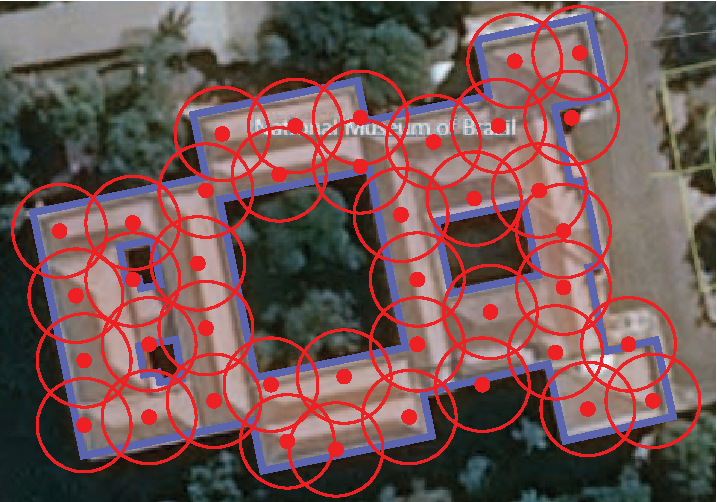
\includegraphics[width=0.95\columnwidth]{chapters/osg/figures/museum-eps-converted-to.pdf}
		\vspace*{1mm}
    \caption{A near-optimal solution for deploying $40$ mobile robots for 
		monitoring the Brazil National Museum, which caught fire in $2019$.}
    \label{fig:osg-museum}
\end{figure}

\section{Conclusion and Discussions}\label{sec:osg-conc}
In this study, we examine \osgt, the problem of directly computing a deployment 
strategy for covering 1D or 2D critical sets using many mobile sensors while 
minimizing the maximum sensing radius. After showing that \osgt is computationally 
intractable to even approximate within $1.152$, we describe several 
algorithmic solutions with optimality and/or computation time guarantees. 
Subsequent thorough evaluation demonstrates the effectiveness of these algorithmic 
solutions. Finally, we demonstrate the utility of our algorithmic solutions with 
two application scenarios. 
%
Due to space limit, guarding perimeters with gaps (see, e.g.,~\cite{fenghangaoyu2019efficient}) 
is not discussed in this work. However, because our algorithms work with a 
grid-based discretization, the results directly apply to arbitrary bounded 1D and 2D 
sets. 

Many intriguing questions follow; we mention two here concerning the sensing 
capabilities. First, \osgt works with circular regions which is perhaps the simplest one
due to symmetry. What if the sensor region is not circular? Whereas such cases 
appear to be hard \cite{culberson1988covering}, effective scalable solutions may 
still be possible. Secondly, currently we assume that all parts of the critical 
set to be guarded have equal importance. What if certain subsets are more important? 




    \chapter{Separating Polygonal Sets with Minimum Sets of Lines}
\thispagestyle{myheadings}

After two chapters' discussion on covering perimeters or regions, which is essentially separating 
some critical polygonal regions from the outside workspace. 
This chapter digs deeper into this problem by studying the separation of more than two regions. 
To simplify the problem, a line-of-sight sensing model will be adopted, where each sensor can cover
an unobstructed line segment like a laser beam. Also, the regions are assumed to be polygonal.

The objective in this case is to minimize the number of sensors used to separate these polygonal sets 
at the existence of obstacles.
% The main objective here is to minimize the number of sensor used.
The problem is NP-hard even for the problem of separating two sets of regions with the minimum number of lines. 
Still, integer programming can provide a near-optimal solution for around 20 objects in a reasonable amount of time. 

\section{Introduction}
Consider the scenario where one or more rogue agents (e.g., criminals) may be hiding in several isolated regions in a 2D workspace. To prevent them from potentially escaping from these regions to other nearby vulnerable regions, we may wish to set up line-of-sight sensors to detect if rogue agents attempt to escape. For the setup, a natural question one may ask is: what is the minimum number of line segments that are needed to form the desired barrier? The same setting finds many other practical applications, for example, for the identical setting, we may use the deployed sensors to track the movement of agents between different set of regions, e.g., understanding the flow of people between residential areas to commercial areas, which can benefit large-scale decision making, e.g., to help properly allocating resources for improving the city infrastructure. 
%
Alternatively, the computed line segments can serve as patrolling routes for autonomous agents (robots or humans) for actively monitoring intrusions, where the agents can always keep tracking events along the segments for which they are responsible.

%Barrier forming \cite{}, i.e. separating multiple sets of objects from each other,
%where each set may contain multiple scattered objects mix among other object sets, finds many real-world applications,
%e.g., erecting security fences around buildings,
%isolating different groups of agents (e.g., people, animals), 
%designing routes for patrolling robots to detect invaders, and so on. 
%multi-agent search for rouge agents, and so on. 
%These applications shares the common objective of better coverage or sensing of the environment with guards. 
%In reality, the types of barriers varies from barriers with range sensibility like lidar, visibility-based barriers like cameras or guards, to physical straight line fences or walls.
%
Motivated by the above-stated scenarios and inspired by earlier research in robotics on barrier forming \cite{kloder2007barrier,kloder2008partial}, i.e., erecting barriers for separating regions of interest, in this chapter, we examine the variation of finding the minimum number of straight line segments for isolating multiple sets of points of polygons in a two-dimensional workspace. 
Fig~\ref{fig:bf-ex}[left] illustrates an instance where three colored polygonal sets are to be separated from each other and the grey polygons are obstacles. Fig~\ref{fig:surf-ex}[right] shows a possible solution which is fairly non-trivial 
to obtain. 
%
%The problem finds applications in many practical scenarios where geometric separation is needed, for example, the deployment of a minimum set of  line-of-sight security beams to guard critical areas from intrusions. 
%dividing different rooms in a floor or buildings from each other to prevent the %spread of virus or contagious diseases,
%designing the surveillance routes for guards that walk on a straight route,
%building fences for regions among different security level that are not allowed 
%to have connections, and so on. 

\begin{figure}[t]
    \centering
    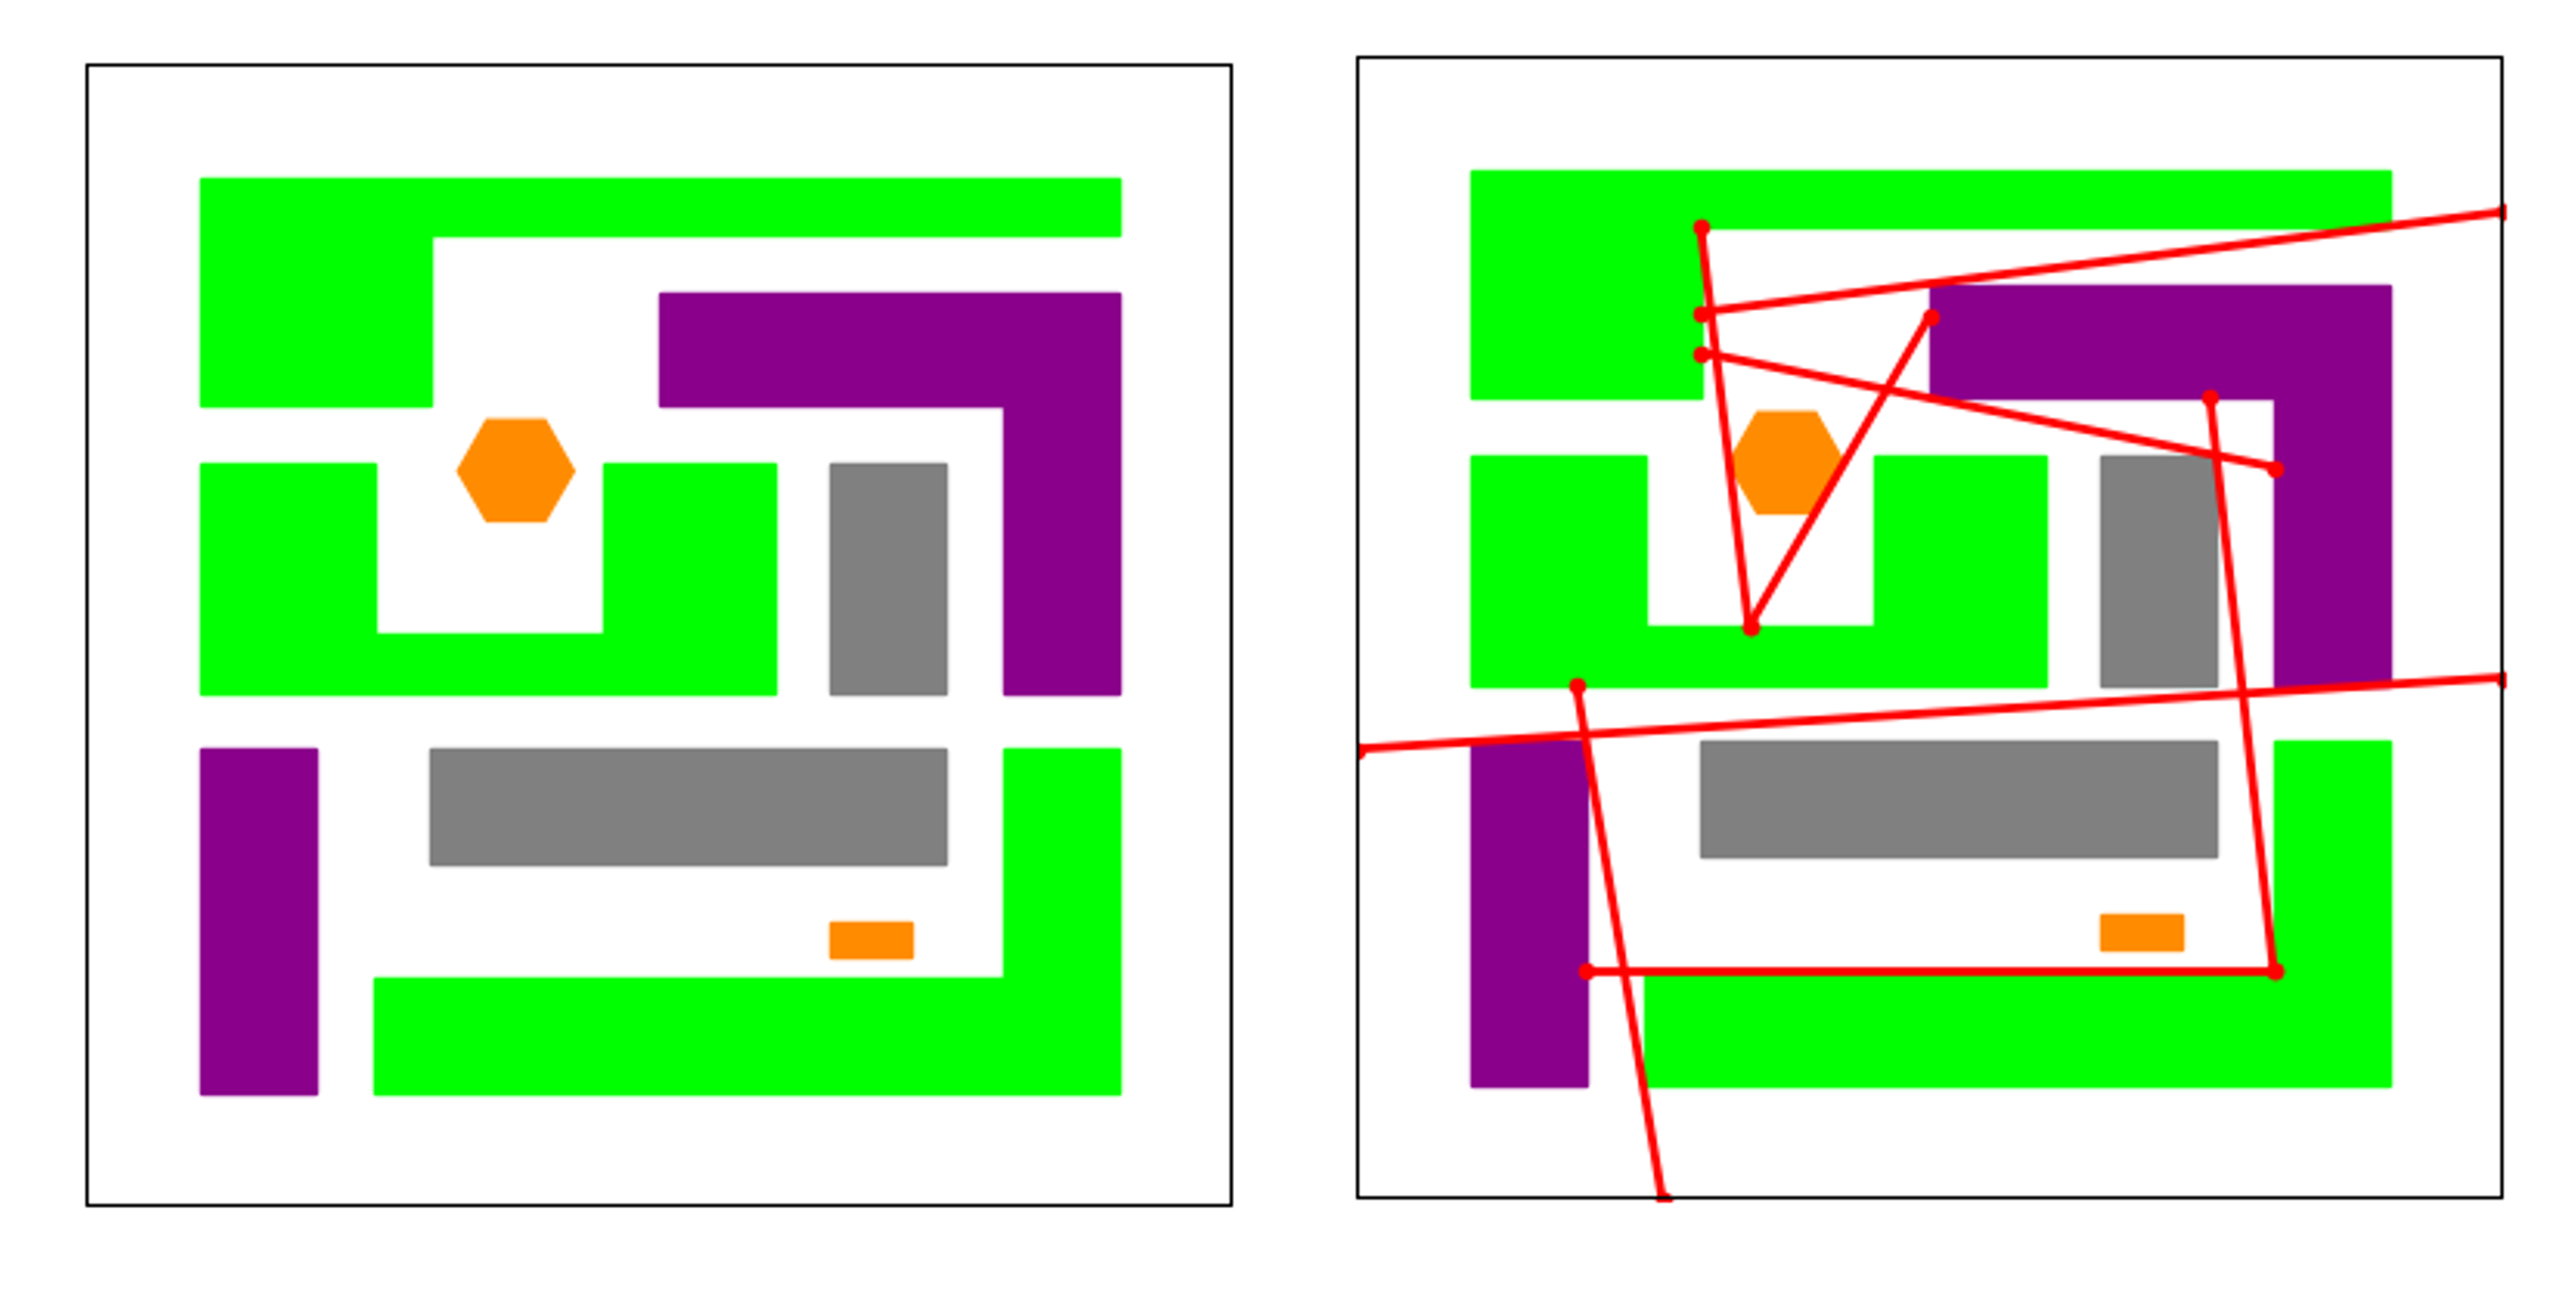
\includegraphics[width=\columnwidth]{chapters/bf/fig/intro_pic.png}
    \caption[Example of barrier forming for separating three sets of complex polygonal shapes]
    {Example of barrier forming for separating three sets of complex polygonal shapes. Different colors represent different sets with the grey ones representing obstacles. The red line segments are the barriers computed by our algorithm.}
    \label{fig:bf-ex}
    \vspace{-0.2in}
\end{figure}
As a summary of this work and its contributions, we study three settings in using line segments to separate sets of disjoint geometric shapes in a 2D workspace: (1) separating point sets, (2) separating point sets among polygonal obstacles, and (3) separating polygonal sets among polygonal obstacles. 
%
Whereas all three settings are NP-hard to optimally solve, we derive an effective method for computing optimal solutions for the first two settings, capable of handling tens of objects (points and/or polygons) partitioned into multiple sets. 
%
The  method first systematically computes candidate barrier set containing a minimum separating barrier, and then builds a novel integer programming model for finding the minimum barrier. 
%
Following a similar approach, we also develop a method that computes solutions for the third set that is proven to be at least $2$-optimal. 
%
We provide a theoretical analysis that sheds some light on why the setting involving polygonal sets is more difficult to solve.
%
Extensive simulation study corroborates the effectiveness of our algorithms. 

%Our contribution to barrier forming is, in summary, formulating the problem of minimizing
%the line segment barriers used with respect to different kinds of object sets (point object and polygonal object). 
%For barrier forming among sets of point objects, we provide effective integer programming based method to obtain the optimal solution.
%For the general polygonal objects, our method can provide a guaranteed 2-OPT solution.
%We also perform evaluations on four different settings to show
%the effectiveness of the proposed method.


\noindent\textbf{Related Work}.
Our investigation of barrier forming has its origins in several research areas.
In the study of pursuit evasion or more generally differential games \cite{ho1965differential,isaacs1999differential,hajek2008pursuit,tovar2009sensor,simov2000pursuit,guibas1997visibility,kameda2006online,kirousis1986searching, sachs2004visibility,lau2005optimal, yu2011shadow, olsen2022robust}, 
% flash light searcher, 1-2 inf searcher
such scenarios often happen where several agents are tasked to search an environment for hidden rogue agents or to protect critical regions from outsider invaders, which amount to creating and maintaining static or dynamic barriers of some form.  
%
Among the approaches taken in finding solutions for these problems, some resort to discretizing the environment into graph representations and conducting search over them \cite{kirousis1986searching, sachs2004visibility}, while others adopt probabilistic reasoning \cite{lau2005optimal, yu2011shadow}. 
%
In particular, Tovar et al. \cite{tovar2009sensor} studied a problem that examines how to untangle sensor beam crossings to reason about the state of a robot, and use the insight to build algorithms for driving a robot to a desired state. In a sense, their study can be viewed as studying a problem that is a dual of the problem that we study here. 

%\textcolor{red}{JJ's edit location}

The barrier forming problem can also be seen as a type of sensor coverage problem. 
%
A series of studies on perimeter defense/guarding problems aim at covering the boundaries of some regions to protect them from the outside \cite{shishika2020cooperative, macharet2020adaptive, fenghangaoyu2019efficient, fengyu2020optimally}, which share similar motivations. 
The barrier forming problem has more flexible solutions by not fixing the specific boundaries to secure the critical regions,
which can be more general and closer to reality in certain cases.
The concept of barrier coverage originates from \cite{gage1992command}, together with the blanket and sweep coverage. 
In \cite{kumar2005barrier}, $k$-barrier was studied. 
In \cite{kloder2007barrier}, the authors solved the min-distance barrier coverage problem optimally under non-trivial environment to minimize the total length of the barriers between two groups of polygonal objects. 
To tackle the proposed problem, a novel and efficient network-flow based method is applied. 
Multiple groups of objects are tackled in \cite{abrahamsen2020geometric}.
The following work \cite{kloder2008thesis} includes a similar problem formation to the problem studied in this chapter, where the objective is minimizing the number of fixed-length line segments used. 
%
However, the proposed method in \cite{kloder2008thesis} uses Tarski sentence \cite{tarski1949decision} which, to our knowledge, does not have a very effective computational tool to deal with.

This work is closely related to several problems in computational geometry, especially point set shattering which seeks a complete separation among a single set of points \cite{freimer1991complexity, har2020separating}. 
Bichromatic point sets or polyhedral separation problem uses wedges, axis-aligned lines, chords, parallel lines, or circles to separate two sets of points or polyhedra \cite{devillers2001separating,armaselu2017geometric,boissonnat2001circular, demaine2005separating}. 
Work on these problems often introduces specific constraints such as working with convex objects or simple polygons without holes, adopting non-crossing or parallel lines as the separator, and so on. 

\noindent \textbf{Chapter Structure}.
The rest of the chapter starts with formulating the barrier formation problem and 
introducing the three variants studied in ~\ref{sec:bf-preliminary}. 
Then, we describe the structure analysis of the problem in ~\ref{sec:bf-structure}, which will base the algorithm
proposed in ~\ref{sec:bf-algorithm}. Lastly, in ~\ref{sec:bf-evaluation} we evaluate the algorithm on four different scenarios. %\r{associate each with a specific section.}

%  methods take
% The problem of constructing a set of barriers appears in various robotics applications 


% Barrier forming is studied in various domains.
% In the pursuit evasion game, barriers were constructed to perform 
% area scan, moving target persuasion \cite{yu2011shadow, tovar2009sensor} etc.
% In computational geometry,
% barrier forming has relevance to several problem: 
% Regarding separating polygons, 
% the study of barrier coverage problem introduces a network flow-based algorithm 
% for computing the minimum total distance separation for two sets of polygons 
% with the existence of obstacles\cite{kloder2007barrier, kloder2008thesis}.
% In \cite{kloder2008thesis}, the author explored barrier forming with minimum number of 
% fixed-length line segments, while it is still important to find high performance
% solution for such problem.\label{sec:bf-intro}

\section{Preliminaries}\label{sec:bf-preliminary}
\subsection{Barrier Forming with Minimum Number of Line Segments}

\begin{figure}[ht]
    \centering
    \vspace{.05in}
    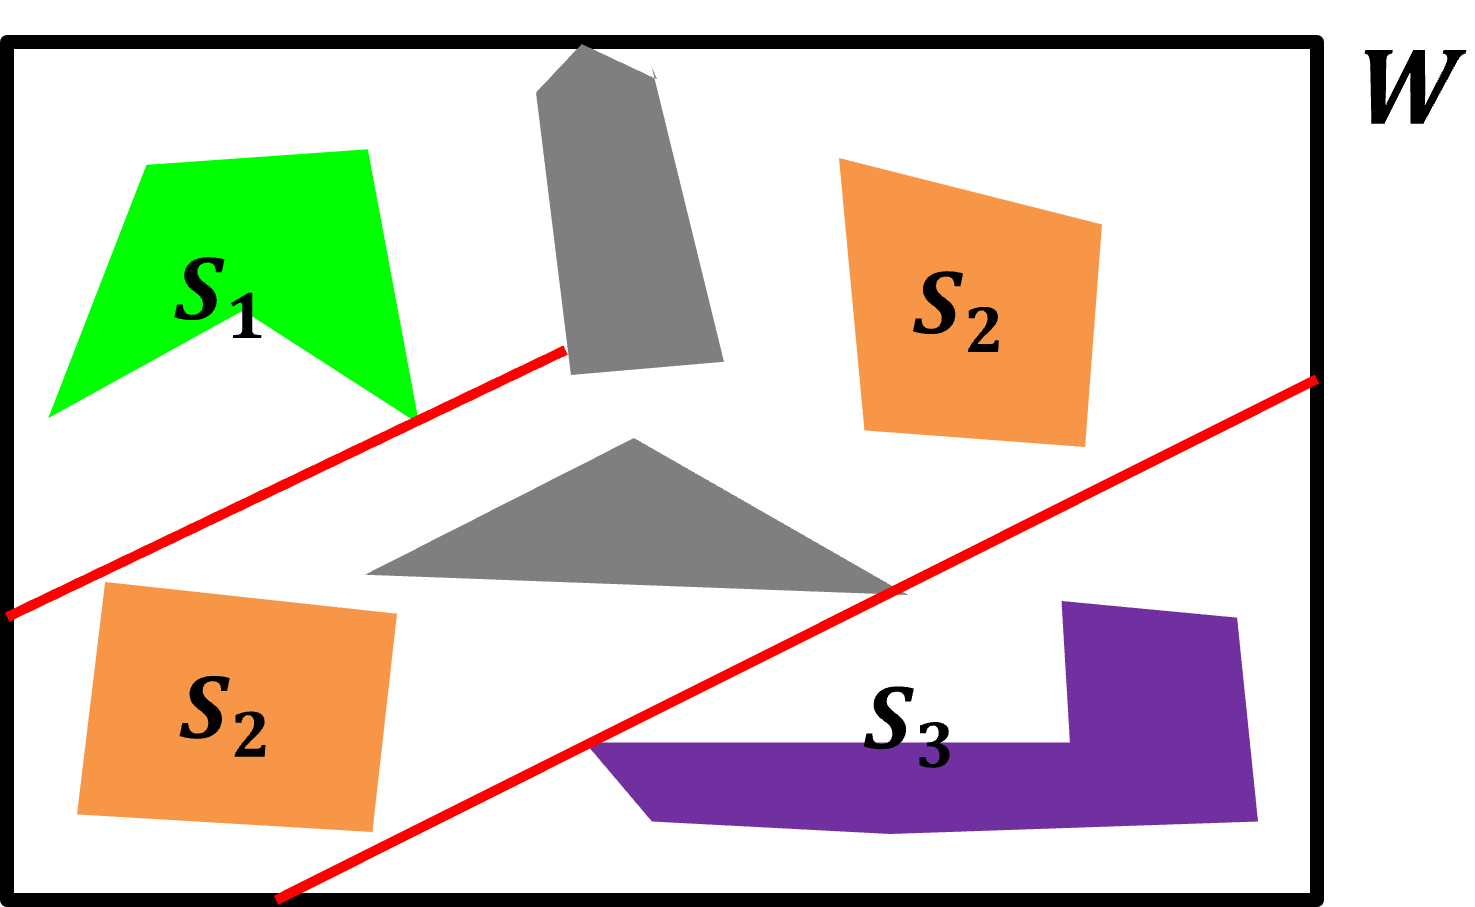
\includegraphics[width = .35\textwidth]{chapters/bf/fig/formulation_pic.png}
    \vspace{.05in}
    \caption[Illustration of a barrier forming problem for the three sets of polygonal objects]
    {Illustration of a barrier forming problem for the three sets of (colored) polygonal objects $S_{1\sim3}$ among (gray) obstacles. 
    For the setting, $2$ straight lines are sufficient to cut off path connections between any pair of polygon regions from two different sets. 
    In this work, our general goal is to build such barriers with the least number of line segments.}
    \label{fig:bf-illustration}
    % \vspace{-0.2in}
\end{figure}

Let $\mathcal{W}$ be a simply connected polygonal workspace in $\mathbb R^2$. Consider $k$ sets of objects $S_1, \dots, S_k$ in $\mathcal W$, as well as a set of polygonal obstacles $\mathcal O$. 
We seek to use a set of straight line segments $L$ to separate $S_1, \dots, S_k$ from each other, such that for any two objects $o_1 \in S_i$ and $o_2 \in S_j, i \ne j$, any path between $o_1$ and $o_2$ in the free space of $\mathcal W$ must be ``cut off'' by one or more line segments from $L$. 
The line segments do not have length limit and can cross each other, but they cannot cross objects or obstacles in the workspace. We want to find the minimum number of line segments to complete the separation task. 

Under the general formulation of Barrier Forming, we examine three different variants with increasing difficulty:
\begin{enumerate} 
\item \emph{Barriers for point sets}, in which  $S_1, \dots, S_k$ as well as $O$ are sets of points. 
\item \emph{Barriers for point sets among polygonal obstacles}, in which  $S_1, \dots, S_k$ are sets of points but $O$ is a set of polygonal objects. 
\item \emph{Barriers for polygonal objects}, in which $S_1, \dots, S_k$ as well as $O$ contain polygonal objects. 
\end{enumerate}
%The first problem considers points sets for separation, that in this case, $S_1, %\dots, S_k$ are point sets, and there are no obstacles in the workspace. This is the %same as the point set separation problem in the plane. 
%The second still takes $S_1, \dots, S_k$ as point set, but introduces polygonal obstacle sets $\mathcal O$ in the workspace. 
%The last one further considers $S_1, \dots, S_k$ as polygonal object sets.

\subsection{Computational Intractability}
Because the separation of even two sets of points in the plane, 
a special case of the first variant of our barrier forming problem, 
is computationally intractable \cite{demaine2005separating}, 
our first formulation is also NP-hard. 
From here, we can reduce from the first variant to other variants involving polygonal shapes by converting each point object to a sufficiently small polygon. Therefore, all three versions of the barrier forming problems studied in this paper are NP-hard. We omit the straightforward details. 

\section{Structural Analysis}\label{sec:bf-structure}

Given that barrier forming problems studied in this work are NP-hard, a natural algorithmic choice for addressing the challenge is through exploring  mathematical programming.
%
To that end, a model must be built that selects from candidate barriers, which in turn requires the construction of a representative set of barrier candidates, a rather non-trivial task. 
%
The set of candidate barriers should satisfy two conflicting constraints: (1) it should contain a minimum set line segments that achieves the desired separation and (2) its size should not be too big that it will cripple the barrier selection process. 
%
Through careful structural analysis, we notice that the barriers to be considered can be limited to \emph{tangent} or \emph{bitangent} line segments. A tangent line segment, with respect to an object or an obstacle, is a line that passes through a vertex or an edge of the object/obstacle but does not intersect its interior. A bitangent is a line segment that is tangent to two objects and/or obstacles. 
%
This allows us to significantly reduce the number of candidates to be examined at the later selection stage.

\begin{theorem}\label{theorem:bf-sin_tan}
For any $k$ sets of polygonal or point objects $S_1, \dots, S_k$ in the workspace $\mathcal W$, the set of line segments that are tangential to the objects and obstacles contains a set of minimum cardinality that separates $S_1, \dots, S_k$. 
\end{theorem}


\begin{proof}

% We prove that there exists a set of lines with minimum cardinality that separates $S_1, \dots, S_k$, and consists of only lines tangent to object vertices. 
Consider a set of line segments $L^*$ with minimum cardinality that separates $S_1,\dots, S_k$. 
Without loss of generality, we assume all line segments in $L^*$ do not end in the free space, i.e., each line segment in $L^*$ ends
at either object boundaries or workspace boundaries.
If some line segment in a minimum barrier is not tangent to any object vertex, denoted it as $\ell=OA$ (shown in ~\ref{fig:bf-proof}), 
we show that it can be replaced by a line segment that is tangent to some object vertex. 
%
Fix one end of $\ell$, $O$ in this case, and rotate $\ell$ around $O$ in both clockwise and counterclockwise directions until it hits some object vertex and becomes tangential to the object.
%
Denote the two line segments resulting from clockwise rotation and counterclockwise rotation as $\ell_1'=OB$ and $\ell'_2=OC$, respectively. 

We show $\ell$ can be replaced with $\ell_1'$ or $\ell_2'$. 
If this is not the case,
since replacing $\ell$ with $\ell_1'$ cannot make the separation work, there must be some point $P_1$ between $AB$ that is path connected to some point in the other class without crossing any line segments in $L^*$ when $\ell$ is replaced with $\ell'_1$. Denote the point as $D_1$ and the path as $path_1$. 
The same analysis goes for $\ell'_2$, that if $\ell$ cannot be replaced by $\ell_2$ then there is some point $P_2$ in $AC$ and path $path_2$ that connects $P_2$ to some other point $D_2$ in a different class and crosses segment $\ell$ but not $\ell_2'$. 
Since there are no objects or obstacles inside triangle $OCB$, we can assume the parts of $path_1$ and $path_2$ inside triangle $OCB$ are straight lines.
So, $path_1$ and $path_2$ must cross each other at some point. 
Denote the cross point as $Q\in path_1 \cap path_2$. 
Then, $path_1 = path_{11} (from\ P_1\ to\ Q) + path_{12} (from\ Q\ to\ D_1)$ and $path_2 = path_{12} (from\ P_2\ to\ Q) + path_{22} (from\ Q\ to\ D_2)$. 
Path $p_{11} + p_{22}$ connects $P_1$ to $D_2$, and $p_{21} + p_{12}$ connects $P_2$ to $D_1$, one of which must not cross $\ell$. 
This leads to a contradiction to the fact that the original line set $L^*$ separates the $k$ classes of objects.

Therefore, each non-tangent line segment in $L^*$ can be replaced with a tangent line segment. 
It will eventually result in a set of tangent barriers with minimum cardinality that separates $S_1,\dots,S_k$.
\begin{figure}[ht]
    \vspace{-2mm}
    \centering
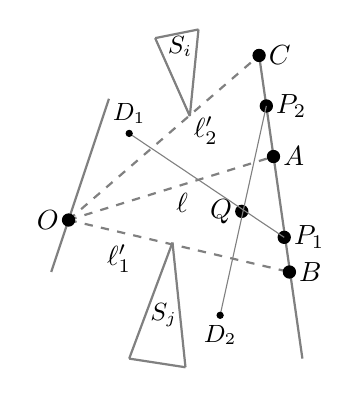
\begin{tikzpicture}[scale = 1.1]
\draw[gray, thick] (0.1, 0) -- (0.7666, 2);
\draw[gray, thick] (3, -1) -- (2.5, 2.5);


\draw[gray, thick] (1, -1) -- (1.5, 0.34);
\draw[gray, thick] (1.65, -1.1) -- (1.5, 0.34);
\draw[gray, thick] (1.65, -1.1) -- (1, -1);

\draw[gray, thick] (1.3, 2.7) -- (1.7, 1.8);
\draw[gray, thick] (1.8, 2.8) -- (1.7, 1.8);
\draw[gray, thick] (1.8, 2.8) -- (1.3, 2.7);

\draw[gray, thick, dashed] (0.3, 0.6) -- (2.66666, 1.333);

\draw[gray, thick, dashed] (0.3, 0.6) -- (2.5, 2.5);
\draw[gray, thick, dashed] (0.3, 0.6) -- (2.85, 0);

\node[text width=1cm] at (2, 0.8) {$\ell$};
\node[text width=1cm] at (2.2, 1.63) {$\ell_2'$};
\node[text width=1cm] at (1.2, 0.15) {$\ell_1'$};

\filldraw[black] (0.3, 0.6) circle (2pt) node[anchor=east] {$O$};
\filldraw[black] (2.666, 1.333) circle (2pt) node[anchor=west] {$A$};
\filldraw[black] (2.5, 2.5) circle (2pt) node[anchor=west] {$C$};
\filldraw[black] (2.85, 0) circle (2pt) node[anchor=west] {$B$};

\filldraw[black] (2.79, 0.4) circle (2pt) node[anchor=west] {$P_1$};
\filldraw[black] (2.5833, 1.917) circle (2pt) node[anchor=west] {$P_2$};

\filldraw[black] (2.3, 0.7) circle (2pt) node[anchor=east] {$Q$};

\draw[gray] (2.79, 0.4) -- (1.0, 1.6);
\draw[gray] (2.5833, 1.917) -- (2.05, -0.5);
\filldraw[black] (1.0, 1.6) circle (1pt) node[anchor=south] {\small{$D_1$}};
\filldraw[black] (2.05, -0.5) circle (1pt) node[anchor=north] {\small $D_2$};


\node[text width=1cm] at (1.9, 2.6) {\small $S_i$};
\node[text width=1cm] at (1.7, -0.5) {\small $S_j$};

\end{tikzpicture}
    \caption{Rotating non-tangent barrier line segment $\ell$ in clockwise and counterclockwise directions around its endpoint $O$ until it becomes tangential to some objects.}
    \label{fig:bf-proof}
    \vspace{-2mm}
\end{figure}
% Then, we show that there exists a set of lines with minimum cardinality that separates $S1$ and $S2$. Similarly, when a line is only tangent to one vertex
\end{proof}

Although we can limit the candidate barriers to line segments tangent to object vertices, there can
still be infinite number of candidates. 
One may consider using line segments that are bitangent to
object vertices, i.e. line segments crossing two object or obstacle vertices. 
If there are $n$ object/obstacle vertices, there can be at most $n^2$, i.e., a quadratic number of bitangents. 
Unfortunately, bitangent lines are insufficient to act as candidate barriers by themselves for polygonal objects. 
A counterexample in ~\ref{fig:bf-counter} shows that there is an instance where an optimal solution must contain line segments that are not bitangents. 
%
In this counterexample, we need separate the orange objects from the lime object. A minimum of three line segments are used, 
and it is not possible that all of them are bitangent, i.e.

\begin{proposition}
Bitangent line segments do not always contain optimal solution for the barrier forming problem for polygonal objects.
\end{proposition}

\begin{figure}[ht]
    \centering
    \vspace{-.2in}
    \includegraphics[width = .25\textwidth]{chapters/bf/fig/counter_example.png}
    \vspace{0.0in}
    \caption{Counterexample that shows using only bitangent line segments cannot create the optimal solution}
    \label{fig:bf-counter}
\end{figure}

Despite the caveat, for the first two formulations that deal with barrier forming for point sets, even with polygonal obstacles, bitangent line segments
always contain an optimal solution. More precisely, 
\begin{theorem}
For any $k$ sets of point objects $S_1, \dots, S_k$ in a workspace $\mathcal W$, there exists
a set of line segments with minimum cardinality that separates $S_1, \dots, S_k$, 
and only consists of bitangent line segments.
\end{theorem}

\begin{proof}
From Theorem~\ref{theorem:bf-sin_tan}, we can see using single tangent line segments is always enough
for an optimal solution. 
Now we turn an optimal solution, $L^*$, with only tangent line segments, into
a solution with only bitangent line segments while still maintaining the same number of barriers. 

For a tangent line segment $\ell=AB\in L^*$ with tangent point $O$ (shown in ~\ref{fig:bf-proof_bi}), and if $O$ is a point object, assume it is beneath $\ell$,
rotate $\ell$ clockwise around $O$ until it hits a point object or an obstacle vertex.
Denote the resulting line segment as $\ell'$, and replace $\ell$ with $\ell'$.
Since the objects are point objects, so $BB'$ and $AA'$ must belong to obstacles or workspace boundary, 
and thus there is no object point inside $OAA'$ or $OBB'$. 
Therefore, the replacement won't result in
any path connecting objects in different classes.
If this is not the case, then there will be some path connecting two object points in different classes that crosses $\ell$ but does not cross $\ell'$ or other barriers. 
Since the triangle areas $OAA'$ and $OBB'$ are empty, that path must enter region $OAA'$ or $OBB'$ and leave them from $\ell$. Then, that part of the path could be replaced with a straight line segment parallel to $\ell$ which prevents it from crossing $\ell$. This contradicts the assumption that $L^*$ prevents all connections between objects in different classes. % of objects.

Continuing the replacement until all line segments are bitangent will result in an optimal solution with only bitangent line segments.

\begin{figure}[ht]
    \centering
    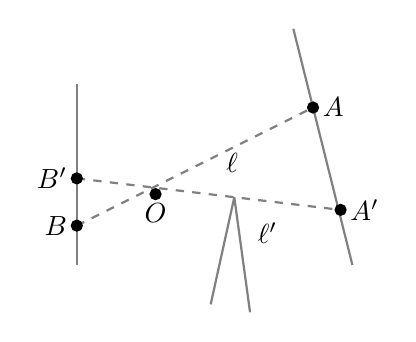
\begin{tikzpicture}
    % \draw[gray, thick] (0, 0) -- (1, 2);
    \draw[gray, thick] (2.5, -1) -- (1.75, 2);
    \draw[gray, thick] (-1, -1) -- (-1, 1.3);

    \draw[gray, thick] (0.7, -1.5) -- (1, -0.14);
    \draw[gray, thick] (1.2, -1.6) -- (1, -0.14);

    % \draw[gray, thick] (3, -1) -- (2.5, 2.5);

    % \draw[gray, thick] (1, -1) -- (1.5, 0.34);
    % \draw[gray, thick] (1.65, -1.1) -- (1.5, 0.34);
    % 
    % \draw[gray, thick, dashed] (0.3, 0.6) -- (2.66666, 1.333);
    \draw[gray, thick, dashed] (-1., -0.5) -- (2., 1.);

    \draw[gray, thick, dashed] (-1., 0.1) -- (2.35, -0.3);

    % \draw[gray, thick, dashed] (0.3, 0.6) -- (2.5, 2.5);
    % \draw[gray, thick, dashed] (0.3, 0.6) -- (2.85, 0);

    \node[text width=1cm] at (1.4, 0.3) 
                            {$\ell$};
    % \node[text] at (1.8, 1.63) 
                            % {$\ell_2'$};
    \node[text width=1cm] at (1.8, -0.6) 
                            {$\ell'$};

    \filldraw[black] (0.0, -0.1) circle (2pt) node[anchor=north] {$O$};
    \filldraw[black] (2, 1.) circle (2pt) node[anchor=west] {$A$};
    % \filldraw[black] (2.5, 2.5) circle (2pt) node[anchor=west] {$C$};
    \filldraw[black] (-1, -0.5) circle (2pt) node[anchor=east] {$B$};

    \filldraw[black] (2.35, -0.3) circle (2pt) node[anchor=west] {$A'$};
    \filldraw[black] (-1, 0.1) circle (2pt) node[anchor=east] {$B'$};

    % \filldraw[black] (2.7583, 0.6666) circle (2pt) node[anchor=west] {$P_1$};
    % \filldraw[black] (2.5833, 1.917) circle (2pt) node[anchor=west] {$P_2$};

    \end{tikzpicture}
    \caption{Rotating a single tangent barrier line segment $\ell$ around its tangent point $O$ clockwise until it becomes bitangent.}
    \label{fig:bf-proof_bi}
\end{figure}
\end{proof}

For separating polygonal objects, although using bitangent line segments cannot guarantee an optimal solution that uses minimum number of line segments, they can still ensure that solutions limited to bitangents are at least $2$-optimal.
\begin{proposition}
For any $k$ sets of polygonal objects $S_1, \dots, S_k$ in the workspace $\mathcal W$, there exists a set of line segments with cardinality at most twice the minimum cardinality, that separates $S_1, \dots, S_k$, and only consists of line segments that are bitangent to object or obstacle vertices. 
\end{proposition}
\begin{proof}


\begin{figure}[ht]
    \centering
    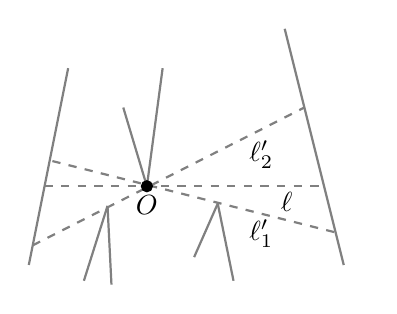
\begin{tikzpicture}

    \draw[gray, thick] (2.5, -1) -- (1.75, 2);
    \draw[gray, thick] (-1.5, -1) -- (-1, 1.5);
    \draw[gray, thick] (0, 0) -- (-0.3, 1);
    \draw[gray, thick] (0, 0) -- (.2, 1.5);

    \draw[gray, thick] (-0.8, -1.2) -- (-0.5, -0.25);
    \draw[gray, thick] (-0.45, -1.25) -- (-0.5, -0.25);

    \draw[gray, thick] (0.6, -0.9) -- (0.9, -0.22);
    \draw[gray, thick] (1.1, -1.2) -- (0.9, -0.22);


    \draw[gray, thick, dashed] (-1.45, -0.75) -- (2., 1.);
    \draw[gray, thick, dashed] (-1.3, -0.0) -- (2.2, 0);

    \draw[gray, thick, dashed] (-1.2, 0.32) -- (2.45, -0.6);



    \node[text width=1cm] at (2.2, -0.2) 
                            {$\ell$};

    \node[text width=1cm] at (1.8, -0.6) 
                            {$\ell'_1$};

    \node[text width=1cm] at (1.8, 0.4) 
                            {$\ell'_2$};

    \filldraw[black] (0.0, -0.0) circle (2pt) node[anchor=north] {$O$};


    \end{tikzpicture}
    \caption{Rotating tangent barrier line segment $\ell$ both clockwise and counterclockwise around its tangent point $O$ until it becomes bitangent.}
    \label{fig:bf-proof_bi_2opt}
\end{figure}

Starting from an optimal solution $L^*$ with only tangent line segments,
we will replace each tangent line segment with two bitangent line segments.

Rotate each non-bitangent line segment $\ell\in L^*$ around its tangent point $O$ in clockwise or 
counterclockwise directions until the line segment become bitangent, 
as illustrated in ~\ref{fig:bf-proof_bi_2opt}. 
Since any path connecting two objects in different classes and is cut by barrier $\ell$ will still be cut by $\ell'_1$ and $\ell'_2$.
The replacement can still guarantee the separation among the object groups.
After replacing all barriers, we can obtain a 2-OPT solution with the number of line segments twice the minimum.
\end{proof}


\section{Fast Computation of High-Quality Solutions}\label{sec:bf-algorithm}
In this section, we will apply the structural results of the barrier forming problem and provide effective method to tackle it.
First, we start with a general method for obtaining the optimal solution among a set of candidate barriers.
Then, based on different ways to generate the candidate barriers, two approaches are given while one is based on 
using bitangent line segments and the other is based on sampling.

\subsection{Optimal Solution for Given Line Separator Candidates}
\label{sec:bf-algo:ilp}
In the barrier forming problem, if the candidate barriers are available as a finite set, we can tackle the problem with integer programming (IP). 
To solve it, we first perform a decomposition of the workspace using the candidate barriers, which partitions the workspace into cells whose edges are part of some candidate barriers. 
Denote  $N$ as the number of candidate barrier line segments, and $M$ as the number of 
cells dissected using the candidate barriers. ~\ref{fig:bf-ilp_example} shows an example of dissecting the workspace into six cells with three candidate barriers.
Then, we can start to construct an IP model to solve the problem of minimizing the number of selected barriers. 
First, we use $\lceil\log k\rceil$ binary variables for each cell, 
resulting in $M\cdot\lceil \log k \rceil$ such variables $c_{11}, \dots, c_{M\lceil\log k\rceil}$. 
The value of $\overline{c_{i1}c_{i2}\dots c_{i\lceil \log k\rceil}}$ will represent the class of cell $i$. 
Thus, if there is an object in cell $i$, $\overline{c_{i1}c_{i2}\dots c_{i\lceil \log k\rceil}}$ should have a fixed value according to the class of the object.
A binary variable for each candidate line segment is used to indicate whether that line candidate is selected,
resulting in $N$ such variables: $\ell_1, \dots, \ell_N$. 

\begin{figure}
    \centering
    \begin{overpic}[width=0.3\textwidth]{chapters/bf/fig/ilp_example.png}
    \put(0, 60) {$\ell_1$}
    \put(40, 95) {$\ell_2$}
    \put(55, 95) {$\ell_3$}
    
    \put(15, 80) {$c_1$}
    \put(50, 75) {$c_2$}
    \put(80, 80) {$c_3$}
    \put(15, 30) {$c_4$}
    \put(50, 15) {$c_5$}
    \put(80, 30) {$c_6$}
    \end{overpic}
    % \includegraphics
    \caption{In this example, we aim to separate two groups of objects with the given candidate barriers. The workspace is decomposed into 6 cells by the 3 candidate barriers. As an example of constraint setup, the pair of adjacent cells $c_1$ and $c_4$ create a constraint of
    $\ell_1\geq c_1 \oplus c_4$, which is equivalent to $\ell_1\geq c_1 - c_4 \wedge \ell_1\geq c_4 -c_1$. (Since there is only $k=2$ classes of objects and $\log k =1$ here, the second index of $c_{i*}$ is eliminated.)} 
    \label{fig:bf-ilp_example}
\end{figure}

Between each pair of adjacent cells $i$ and $ j$ (let the candidate line segment between them correspond to $\ell_\sigma$), we have ($\oplus$ denotes ``exclusive or'')
\begin{equation}
\begin{split}
    &\ell_\sigma \geq c_{i\tau} \oplus c_{j\tau}  \Leftrightarrow \ell_\sigma \geq c_{i\tau} - c_{j\tau} \wedge \ell_\sigma\geq c_{j\tau} - c_{i\tau}, \\
    &\text{  for each adjacent cell $i$, $j$, and $1\leq \tau \leq \lceil \log k \rceil$},
\end{split}
\end{equation}
which means if two adjacent cells belong to different classes, then the line segment candidate between them must be selected. 
An example of the constraint setup is illustrated in ~\ref{fig:bf-ilp_example}.
Naturally, we have fixed $c_{i1},\dots,c_{i\lceil \log k\rceil}$ if ceil $i$ contains an object to be separated, 
and the value of $\overline{c_{i1}c_{i2}\dots c_{i\lceil \log k\rceil}}$ is set to be the same as its class index: $0\sim k-1$.
The objective is set to minimize the total number of line candidates selected, i.e., $\min \sum_{i=1}^{M} l_i$.

\subsection{Near-optimal Solution Using Bitangent Lines}
As the results in Section~\ref{sec:bf-structure} show, using bitangent line segments 
can always provide optimal solution for the problem of barrier forming for point objects, 
and at least 2-OPT
solution for separating polygonal objects. 
Since the number of bitangent line segments is at 
most quadratic to the number of object or obstacle vertices, 
we can enumerate them, and apply IP method in Section~\ref{sec:bf-algo:ilp} to find a solution. 
~\ref{fig:bf-barrier_candidates} illustrates the candidate barriers constructed for point objects and polygonal objects.
It is worth noting that for enumerating bitangent barriers for point objects, the side of the point to the barrier also matters. 
For example, a pair of point objects will create $4$ bitangent barrier candidates as there are 4 different possible cases depending on the how the corresponding objects are placed with respect to the line. 

\begin{figure}[ht]
    \centering
    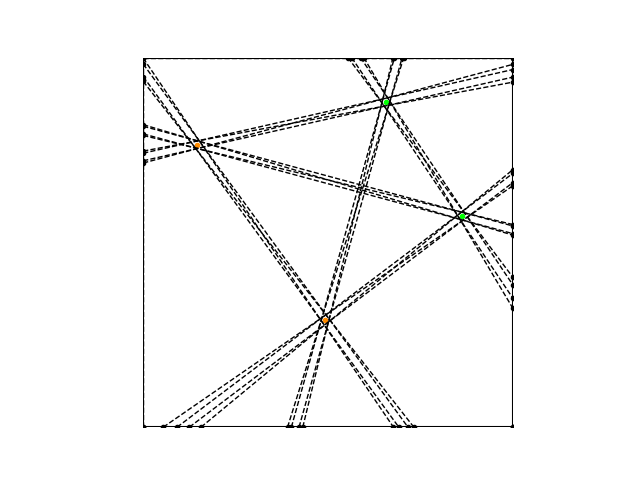
\includegraphics[trim=80 20 80 20,clip, width = .24\textwidth]{chapters/bf/fig/candidate_1.png}
    \hspace{-.1in}
    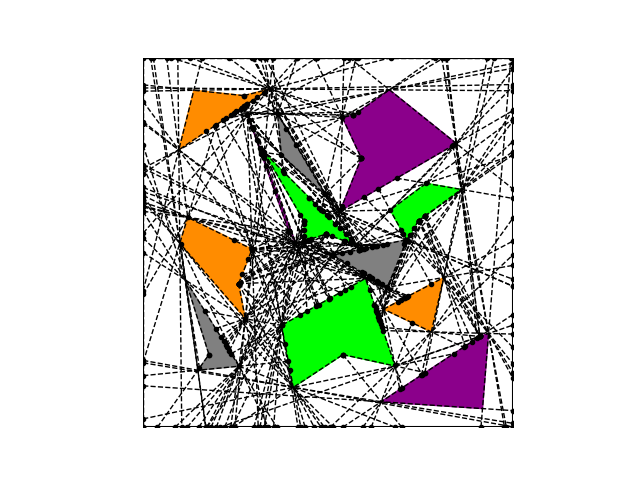
\includegraphics[trim=80 20 80 20,clip, width = .24\textwidth]{chapters/bf/fig/candidate_2.png}
    \caption{Illustration of bitangent barrier candidates. The left picture shows the bitangent
    candidates for $2$ point sets, each with $2$ points. In this case, a pair of points will create $4$ candidates. 
    We note that we made the points non-zero-dimensional for visibility purposes. 
    The right picture shows the bitangent candidates for $12$ polygonal objects in four sets.}
    \label{fig:bf-barrier_candidates}
\end{figure}

\subsection{Sampling-based Resolution Complete Algorithm}
Although using bitangent line segments works well in most of the cases, it unfortunately cannot provide an optimal guarantee for the barriers formed when dealing with polygonal objects.
However, theorem~\ref{theorem:bf-sin_tan} provides a good starting point for sampling line segments: we may limit candidate barrier sets to single tangents, 
i.e., we sample line segments passing through each object vertex in a radial manner. 
Hence, if we gradually increase the sampling resolution around each object and obstacle vertex and use the sampled line segments as candidate barriers, 
we can guarantee the asymptotic optimality of the resulting solution.

% In this section, we first describe a polynomial time approximation algorithm for a restricted version of Problem~\ref{p:2}. Then, we describe a general integer linear programming framework for solving Problems~\ref{p:1}-\ref{p:3},
% and local improvement techniques for enhancing solution quality.

% \subsection{Polynomial Time Approximation Algorithm}
% % Briefly mention the hardness results
% % As for 2D OSG, it is similar to the metric k-center problem and therefore
% the approximation algorithms solving k-center problem can be applied to 2D OSG. 

In their general forms, Problems~\ref{p:1}-\ref{p:3} require the computation of 3D visibility, a hard task on its own. Due to this reason, a polynomial time algorithm with guaranteed good approximation ratio for these problems appear difficult to come by. It is an interesting question to ask whether some form of approximation scheme can be derived. Here, we show that for Problem~\ref{p:2}, if one relax the visibility requirement, i.e. letting $vis(\cdot, \cdot)\equiv 1$, then a polynomial time $(2+\varepsilon)$-approximation algorithm can be obtained. 

Taking Problem~\ref{p:2}, we examine a setup assuming that each point $p \in S$ has good visibility, i.e., $p$ is always visible to the nearest sensor. Such scenarios happen when the 3D domain does not have large curvatures that would easily block sensors' view, e.g., covering the earth with GPS satellites or using drones to survey a vineyard. To drive a specific approximation bound, 
we further assume that sensors have spherical range sensing and are in a plane of some fixed 
\begin{wrapfigure}[5]{r}{1.3in}
  \vspace*{0mm}
  \begin{overpic}[width=1.3in,tics=5]{chapters/surf/fig/env.png}
	\end{overpic}
\vspace*{-6.5mm}
\end{wrapfigure}
height $h$ from the ground, which may be relaxed. Denote this surface as $H_C$. 
The figure on the right provides an illustration of the target environment setting. 

The main idea is to first obtain a dense sample of $S$ and then adapt $2$-approximation algorithms for the corresponding 2D setting, which requires some non-trivial reasoning. Two well-known approximation algorithms for $k$-center like problem in 2D are based on \emph{farthest point clustering} \cite{gonzalez1985clustering} and \emph{dominating set} \cite{hochbaum1985best, vazirani2013approximation}. Both of these approaches work for our purpose; we show how to work with the former.

Let a uniformly sampled set of point of $S$ be $S_N = \{o_1, \ldots, o_N\}$. We apply farthest point clustering \cite{gonzalez1985clustering} on $S_N$ as follows. As the name suggest, it picks farthest sensor locations until the number of sensors are exhausted. In the original approach, the points to be clustered are also sensor locations, which is not true here. Instead, we perform clustering in the set $S_N$ and project the selected samples to $H_C$ gradually. The relatively straightforward process is given in Algorithm~\ref{alg:greedy} (($d(\cdot$,$\ \cdot)$ denotes the distance between the inputs, one or both of which may be sets).


\begin{algorithm}
\begin{small}
    \SetKwInOut{Input}{Input}
    \SetKwInOut{Output}{Output}
    \SetKwComment{Comment}{\% }{}
    \caption{Farthest Point Clustering}
		\label{alg:greedy}
    \SetAlgoLined
		\vspace{1mm}
    \Input{$S_N$=\{$o_1, \dots, o_N$\}: $N$ sampled points on the surface $S\subset \partial \mathcal E$; $k$: number of sensors;\\
    $H_C$: a plane with a fixed height}
    \Output{$\mathcal{C}$: sensor location set}
		\vspace{1mm}
        % $\mathcal C$ = $\varnothing$\\
        $\mathcal{C} \leftarrow$  \{$o_1$'s vertical projection onto $H_C$\}\\
        % \While{$|\mathcal{C}|<k$}{
        \For{$i \gets 1$ \KwTo $k$}{
        \For{$o\in S_N$}{
        compute the distance $d(o, \mathcal{C})$ between $o$ and $\mathcal{C}$\\ 
        }
        $o \leftarrow$ point $v\in S_N$ with the largest $d(v,\mathcal{C})$\\
        $\mathcal{C} \leftarrow \mathcal{C}\ \cup \{o$'s projection onto $H_C$\}\\
        % $p^\star \leftarrow$ the projection of $v^\star$ on height $H$\\
        % Add $p^\star$ to $\mathcal{C}$\\
        }
        \Return $\mathcal{C}$
\end{small}
\end{algorithm}

To prove the claimed $(2+\varepsilon)$-approximation bound,  
denote the optimal sensor location set and the sensor location set derived by Algorithm~\ref{alg:greedy} as $\mathcal{C}_{OPT}$ and $\mathcal{C}$, respectively. Since these are centers of spherical sensing ranges, we call them center set for short. Denote the minimum coverage radius in the spherical sensing model as $r_{OPT}$. Let $h$ be the minimum distance between surface $S$ and sensor space $H_C$, i.e. $h:=d(S,H_C)$. $r_{OPT}$ and $r_{\mathcal{C}}$ are defined as follows:
\begin{equation}
    r_{OPT}:=\max_{o\in S_N} d(o, \mathcal{C}_{OPT})
\end{equation}
\begin{equation}
    r_{\mathcal{C}}:=\max_{o\in S_N} d(o, \mathcal{\mathcal{C}})
\end{equation}

\begin{proposition}
\label{prop:algo1t}
The center set obtained by Algorithm~\ref{alg:greedy} achieves coverage radius of at most
%$r_{OPT} + \sqrt{r_{OPT}^2 - h^2}$
$\sqrt{4r_{OPT}^2 - 3h^2}$.
\vspace{-1mm}
\end{proposition}
\begin{proof}

%So we need to prove:
%\begin{equation}
%    r^{C}\leq 2r^{OPT}
%\end{equation}

Denote the center set generated at the 
$i$th round as $\mathcal{C}_{i}$, and $r_i$ as the cluster radius $r_i := \max_{o_\tau}\min_{c_j \in \mathcal{C}_i} d(o_\tau, c_j)$. It is straightforward to observe that $r_k\leq r_{k-1} \leq \dots \leq r_1$.
Consider the relationship between the optimal center set $\mathcal{C}_{OPT}$ and the center set obtained by Algorithm~\ref{alg:greedy}, we have the following 2 cases.

Case 1: For each sphere $\mathcal{B}_{c}$ centered at a point $c\in\mathcal{C}_{OPT}$ with radius of $r_{OPT}$, the projection of $\mathcal{B}_{c}\bigcap S$ onto the sensor space $H_C$
contains exactly one point of $\mathcal{C}_k$. 

% \kg{KG: Since we have a projection step, the OPT sphere needs to cover not only the center, but also the points that project to the center}

In this case, let $v$ be an arbitrary point in $S$. 
Let $c_{\alpha}$ be the nearest center to $v$ in $\mathcal{C}_{OPT}$ 
and $c_{\beta}$ be the point in $\mathcal{C}_k$ whose projection on $S$ is inside $\mathcal{B}_{c_{\alpha}}$. 
Therefore, we have: 
\begin{equation}
    d(v, c_\beta) 
    % \leq d(v,c_{\alpha}) + d(c_{\alpha}, c_\beta) 
    \leq 
    %r_{OPT} + \sqrt{r_{OPT}^2-h^2}
    \sqrt{4r_{OPT}^2 - 3h^2}
\end{equation}

Case 2: There exists a sphere $\mathcal{B}_{c}$ centered at a point $c\in\mathcal{C}_{OPT}$ with radius of $r_{OPT}$, the projection of $\mathcal{B}_{c}\bigcap S$ onto the sensor space $H_C$
contains at least 2 points of $\mathcal{C}_k$. 
In this case, denote the two centers by $c_i$ and $c_j$ $(i<j)$, and their projections on $S$ are in the same sphere $\mathcal{B}_c$. As $c_j$ is added after $c_i$, then,
%Without loss of generality, we can assume that $c_2$ is added in the $i^{th}$ iteration and is no less than $c_1$.% then we have:
\begin{equation}
    \begin{split}
    r_\mathcal{C} = r_k 
    &\leq r_{j}
    \leq d(c_i, c_j\text{'s projection on } S)\\
    &\leq \sqrt{4r_{OPT}^2 - 3h^2}
    % \\
    % &\leq \sqrt{r_{OPT}^2 - h^2} + r_{OPT}\\
    \end{split}
\end{equation}
Summarizing the two cases proves Proposition~\ref{prop:algo1t}.
\vspace{-2mm}
\end{proof}

% \begin{remark}
% With a finer analysis, it can be shown both approximation algorithms are guaranteed to produce at most $\sqrt{4r_{OPT}^2 - 3h^2}$ spherical radius.
% \end{remark}
\vspace{-0.05in}

% \vspace{-2mm}
% \subsection{Integer Programming-Based Algorithmic Framework}
% With Problems~\ref{p:surf-1}-\ref{p:surf-3} being computationally intractable, a natural algorithmic alternative is mathematical programming. In \cite{fengyu2020optimally}, an integer linear programming (ILP) model was shown to be effective for a 2D setting. For our 3D problems, visibility constraints must be effectively handled. We pre-compute pairwise visibility at a given sample granularity. The information is then fed to an ILP model. As the discretization granularity gets smaller, we can then realize \emph{globally optimal} $(1\pm \varepsilon)$-approximations (depending whether it is a maximization or a minimization). 

As a first step to building the ILP model, visibility information must be computed. 
We work with two discretizations, the surface $S$ to be covered and the space where the sensors may be deployed (as discussed in Section~\ref{sec:surf-preliminary}, this is a 3D space though in practice it is frequently a 2D subset). For each pair of samples, we use a collision checker \cite{cgal:aabb-20b} to determine whether the line segments between the two samples intersects $\mathcal E$. During the process, we also compute for each sample $p\in S$ its normal $\hat{n}_p$.

%For the actual computation, we first work only with samples of $S$. For each sample $p \in S$, we then sample the $2$-sphere $\mathbb S^2$ around $p$ to get a unit vector $\vec{v}$. For each $(p, \vec{v})$, we compute the point $p' \in \mathcal E$ that blocks the ray starting at $p$ in the direction of $\vec{v}$. This information is then used to compute pairwise visibility information between the surface samples and sensor location samples. Such an approach decouples the visibility computation between the two sample sets. 

%
With the visibility pre-computation performed, we are ready to construct the ILP models. For all three problems, recall that we have $S_N = \{o_1, \ldots, o_N\}$ for discretizing the surface $S$ through grid-based sampling. 
We use boolean variable $y_i$ to indicate whether sample $o_i$ is covered. 
Candidate sensor locations are also discretized to obtain a sample set $\{c_1, \ldots, c_M\}$, from which $k$ locations would be selected with $z_i$ indicating whether $c_i$ is selected. 
The ILP model for the Problem~\ref{p:surf-1} is
\begin{gather}
    y_i   \leq \sum_{j\ s.t.\ vis(o_i, c_j) = 1} z_j   \text{\quad for each } o_i\\
    \sum_j z_j \leq k\\
    \max\ \ y_1 + \dots + y_N
\end{gather}


%In the integer linear problem framework, we first discretize the candidate 
%robot locations using grids. 
%Then, pairwise sensing quality was computed between each pair
%of candidate sensor location and sampled points on the surface. 
% So, we can obtain the 
% following integer programming model to approximately computing the maximum number 
% of surface being computed.
%In these models, we have $N$ samples on the surface $\{o_1, \dots, o_N\}$ and $y_i$ indicates whether sample $o_i$ is covered. Also, there are $M$ candidate sensor locations $\{c_1, \dots, c_M\}$ and $z_j$ indicates whether $c_j$  is selected as sensor location.
%For the visibility model, we have the following integer programming model. 
%\begin{gather}
%    y_i   \leq \sum_{j} vis(c_j, o_i)\cdot y_i   %\text{\quad for each } o_i\\
%    \sum_j c_j \leq k\\
%    \max\ \ y_1 + \dots + y_N
%\end{gather}

The cumulative quality case (Problem~\ref{p:surf-3}) is similar. Denoting the sensing
quality between sensor location $c_j$ and surface point $p$ 
as $\phi(p, c_j) = vis(p, c_j) \cdot (
\hat{n}_p, \hat{n}_{p c_j} )/||p c_j||^2$, the ILP model may be constructed as

\begin{gather}
    y_i \cdot \Phi  \leq \sum_{j} \phi(o_i, c_j)\cdot z_j   \text{\quad for each }o_i\\
    \sum_j z_j \leq k\\
    \max\ \ y_1 + \dots + y_N
\end{gather}

% Reason for comment, 
% We note that although $\phi(o_i, c_j)$ is computed as a floating 
% point value, using such values significantly increases computational 
% burden. Therefore, in transferring the values to the ILP model, 
% we further discretize $\phi(o_i, c_j)$ to be an integer within some 
% certain range, e.g. $0\sim 10$.

For quality maximization (Problem~\ref{p:surf-2}), the objective is to maximize 
the minimum distance of a sampled point on the surface to its nearest sensor 
location. 
%If we further consider visibility here, then if there exists a point 
%that is not visible to any deployed sensor, then the objective can never be 
%%positive. So, its more natural to apply this formulation to scenarios where no
%visibility issues were raised. 
For a required coverage ratio $\rho$ and radius $r$, we can verify whether it is possible to put $k$ sensors and cover $N\rho$ discretized points by checking the 
feasibility of the following model:
% Then, the essentially same method as our previous work can be applied. 
\begin{gather}
    y_i \leq \sum_{j\ s.t.\ ||c_j - o_i|| \leq r}  z_j \text{\quad for each } o_i\\
    \sum_j z_j \leq k\\
    N \rho \leq \sum_i y_i 
    % \max\ \ y_1 + \dots + y_N
\end{gather}
A subsequent binary search can be applied to find the smallest feasible $r$. 
%When $\rho = 1$, the optimization is applied to all visible points in $S_N$ 
%to $k$ sensors.
%\sw{all points in S\_N ?}



% \vspace{-1mm}
% \subsection{Local Enhancement of Coverage Quality}
% %\sw{``Enhancing Coverage Quality Locally" instead ?}
% Whereas the ILP models for Problems~\ref{p:1}-\ref{p:3} support arbitrary precision, given that these problems are all computationally intractable, it can be expected that a pure ILP-based solution will only be scalable up to a certain point before an exorbitant amount computation time is needed. Inspired by the iterative update approach form \cite{cortes2004coverage}, we propose a two-phase optimization pipeline of using ILP (or the approximation algorithm for Problem~\ref{p:2}) as the first phase with a good level of \emph{global} optimality guarantee and follow that with \emph{local} improvements that can be quickly computed to enhance the initial solution. We note that, as the local improvement is enhancing a solution with a level of global optimality guarantee, the enhancement is also global in effect. For example, in Problem~\ref{p:2}, if we start with a $2$-approximation solution and obtain an initial coverage quality $r$ and subsequent local improvement reduce that to $0.75r$, then the final solution is a globally $1.5$-optimal solution.

We develop two such routines. The first is generally applicable and straightforward to implement: as the discretization level increases, we move the set of initial sensor locations (computed by Algorithm~\ref{alg:greedy} or ILP) locally, one at a time. More formally, given an initial solution $\mathcal C = \{c_1, \dots, c_k\}$, denote $S_j \subset S$ as the region covered (possibly partially when working with Problem~\ref{p:3}) by the sensor deployed at $c_j$. For each $S_j$, we try improving the quality of the solution by finding a better location for $c_j$ to cover $S_j$ at a finer resolution. Subsequently, $S_j$ can be updated based on the new $c_j$. The process may be repeated until convergence. 

The second local improvement routine is via solving a ``1-cener'' like problem and is applicable to Problem~\ref{p:2} and Problem~\ref{p:3}. Due to limited space, we omit the lengthy algorithmic details and give a high-level description. For Problem~\ref{p:2}, a sensor located at $c_j$ is ``responsible'' for visible points of $S$ that falls within a ball $B(c_j, r)$. Our improvement routine examines $S \cap B(c_j, r)$ and attempts to compute a new ball with a smaller radius that covers all of $S \cap B(c_j, r)$. The routine uses the ideas from Welzl's algorithm for computing minimum enclosing discs \cite{welzl1991smallest, Mark1997computation} and take time that is expected linear with respect to the number of samples that falls within $B(c_j, r)$, which is fairly fast. This method can be readily extended to Problem~\ref{p:3} where the spheres become ``distorted'' (Fig.~\ref{fig:exposure}).


\section{Experimental Evaluation}\label{sec:bf-evaluation}
In this section, we describe our experimental study of the method proposed in the paper.
Four settings were used to account for the three variants of the barrier forming, the instances and solution examples of which are shown in ~\ref{fig:bf-exp}. 
The experiments were carried out on a Hexa-Core processor with 16 GiB memory, and Gurobi
\cite{optimization2019gurobi} was used as the Integer Programming solver.
In the polygonal object instances generation, random polygons were generated by computing traveling salesperson tour (TSP) tours of random point sets each consisting of $3$ to $6$ vertices, which we found to be effective in generating sensible looking polygons that are not necessarily convex.
%
When a problem setup contains obstacles, the number of obstacles in the environment is set to be the same as the number of objects for each object set.


\begin{figure*}[ht]
    \centering
    
    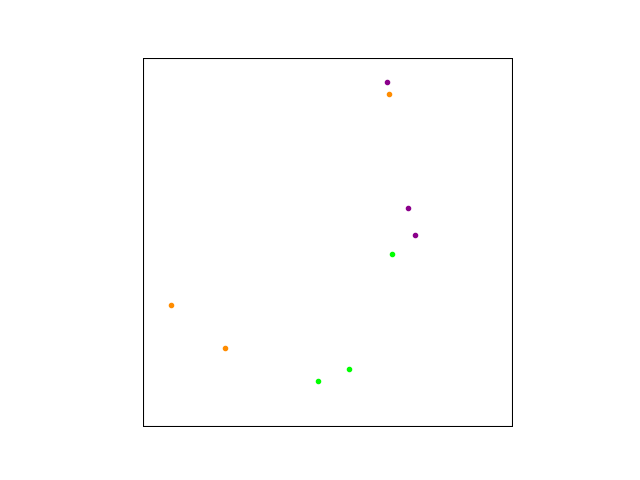
\includegraphics[trim=80 20 80 20,clip, width = .24\textwidth]{chapters/bf/fig/exp_1_instance.png}
    \hspace{-.1in}
    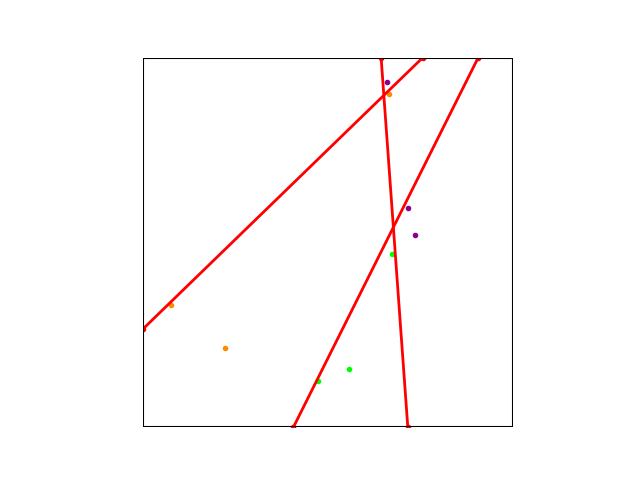
\includegraphics[trim=80 20 80 20,clip, width = .24\textwidth]{chapters/bf/fig/exp_1_result.png}
    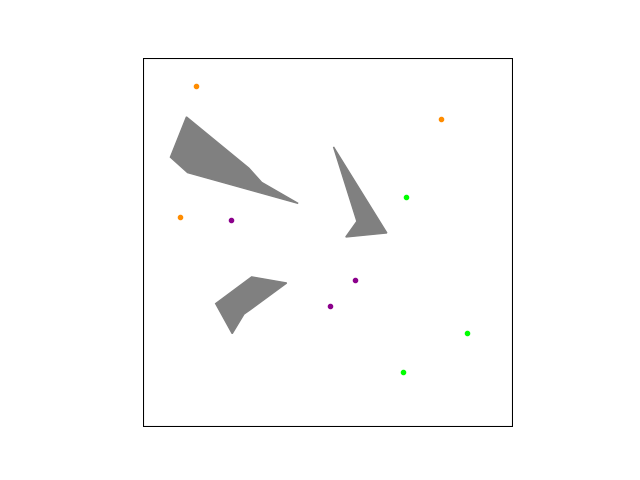
\includegraphics[trim=80 20 80 20,clip, width = .24\textwidth]{chapters/bf/fig/exp_2_instance.png}
    \hspace{-.1in}
    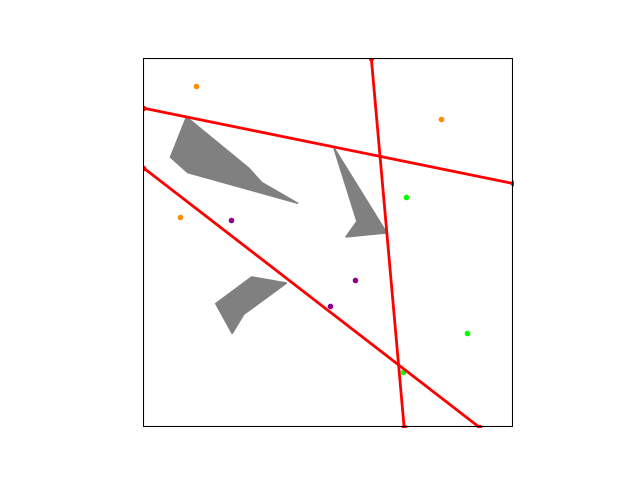
\includegraphics[trim=80 20 80 20,clip, width = .24\textwidth]{chapters/bf/fig/exp_2_result.png}
    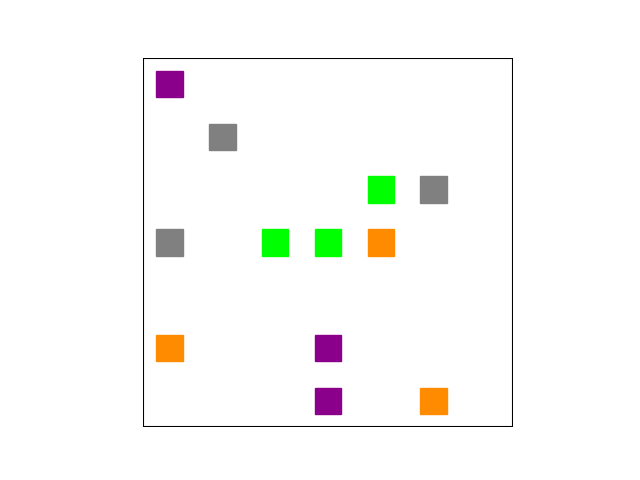
\includegraphics[trim=80 20 80 20,clip, width = .24\textwidth]{chapters/bf/fig/exp_3_instance.png}
    \hspace{-.1in}
    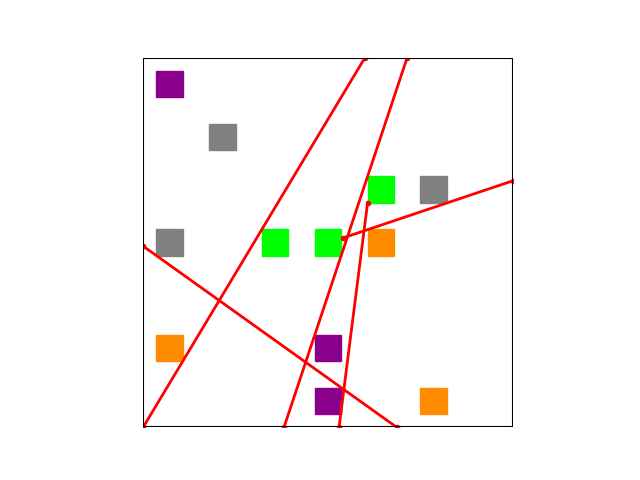
\includegraphics[trim=80 20 80 20,clip, width = .24\textwidth]{chapters/bf/fig/exp_3_result.png}
    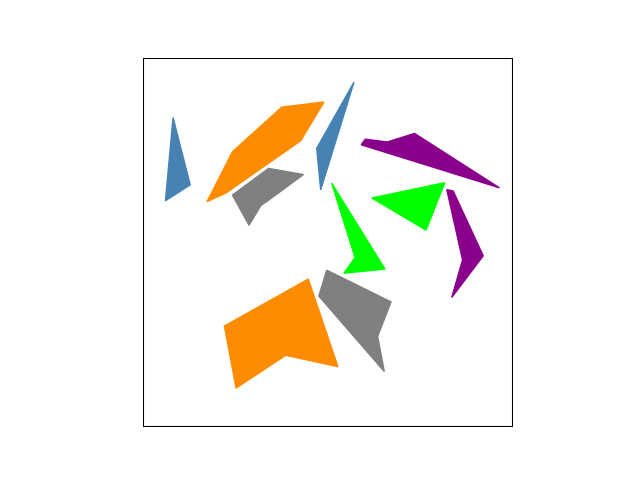
\includegraphics[trim=80 20 80 20,clip, width = .24\textwidth]{chapters/bf/fig/exp_4_instance.png}
    \hspace{-.1in}
    % 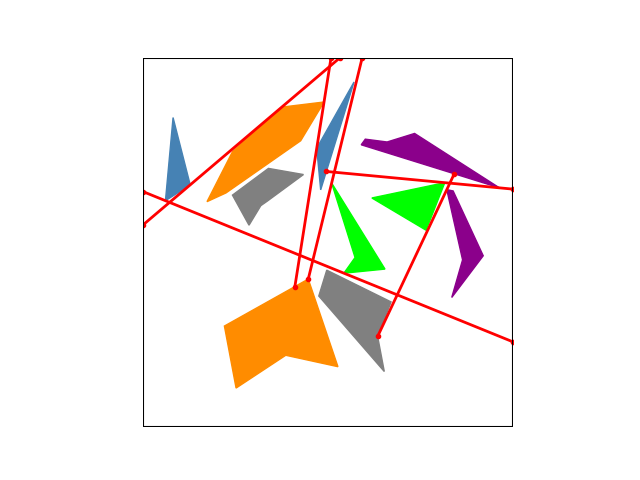
\includegraphics[trim=80 20 80 20,clip, width = .24\textwidth]{fig/exp_4_result.png}
    \begin{overpic}[trim=80 20 80 20,clip, width = .24\textwidth]{chapters/bf/fig/exp_4_result.png}
    \put(-202, 98) {(a)}
    \put(-3, 98) {(b)}
    \put(-202, 0) {(c)}
    \put(-3, 0) {(d)}
    
    \end{overpic}
    \caption{Illustration of the four types of instances used in our  experimental evaluation. (a) Barrier forming for point sets. (b) Barrier forming to separate point sets from polygonal obstacles. (c) Barrier forming to separate uniform square-shaped objects among uniform square-shaped obstacles. (d) Barrier forming to separate random polygonal objects among random polygonal obstacles.}
    \label{fig:bf-exp}
\end{figure*}

\subsection{Separating Sets of Points}
The first type of instances aims at forming barriers among randomly generated point sets, 
shown in ~\ref{fig:bf-exp}(a). The number of object sets to separate from each other range from $2$ to $4$, 
and the number of objects in each set range from $1$ to $6$. 
Each entry in the ~\ref{tab:bf-expr_1} is the result of average computation times over 10 instances. From the result, we observe that the IP based method is fairly effective in separating two sets of objects with the presence of obstacles. The method scales to about $10$ point objects plus obstacles. The number of line segments in the optimal barrier are generally small, e.g., $3$-$10$.

\begin{table}[ht]
    \centering
    \begin{tabular}{|c|c|c|c|c|c|c|}\hline
        %  \diagbox{\#Set}{\#Objects}
        \#Sets &  1 & 2 & 3 & 4& 5& 6\\\hline
 2& 0.005 & 0.011 & 0.083 & 0.419 & 2.010 & 15.887 \\\hline
 3& 0.013 & 0.316 & 12.773 & 962.883 & - & - \\\hline
 4& 0.051 & 14.641 &  -& - &  -&- \\\hline
\end{tabular}
    \caption{Running time in seconds for Expr. 1 where all objects and obstacles are points (~\ref{fig:bf-exp}(a)). ``-'' denotes the result cannot be computed in 1h on average (the same is true for other tables). 
    The column index means the number of objects in each set, and the row index means the number of object sets.
    The number of obstacles is set to be the same as the number of objects for each set. These also apply to the following tables.
    }
    \label{tab:bf-expr_1}
\end{table}

 The second type of instances generates barriers for randomly generated 
 point sets with the existence of polygonal obstacles, shown in ~\ref{fig:bf-exp}(b). 
 The other specification is the same as Expr. 1, and the number of obstacles for each experiment is set to be the same as the number of objects for each set. 
 The resulting time cost, shown in \ref{tab:bf-expr_2}, is similar to Expr. 1 despite the existence of obstacles.
 %
 Similarly, we observe decent performance when it comes to separating two sets of objects among obstacles. 
 %
 The introduction of polygonal obstacles does not cause performance degradation. 


\begin{table}[ht]
    \centering
    \begin{tabular}{|c|c|c|c|c|c|c|}\hline
        %  \diagbox{\#Set}{\#Objects}
        \#Set &  1 & 2 & 3 & 4& 5& 6\\\hline
2& 0.009 & 0.061 & 0.480 & 5.899 & 3.433 & 21.121\\\hline
 3& 0.044 & 3.287 & 71.346 & 320.955 & - & -\\\hline
 4& 0.249 & 13.801 & - & - & - & -\\\hline
    \end{tabular}
    \caption{Running time in seconds for Expr. 2 where objects to be separated are points and obstacles are randomly generated polygons (~\ref{fig:bf-exp}(b)). 
    }
    \label{tab:bf-expr_2}
    \vspace{-2mm}
\end{table}
 
\subsection{Separating Sets of Polygonal Shapes}
The third set of experiments uses randomly placed squares as obstacles and objects, shown in ~\ref{fig:bf-exp}(c). The squares are sampled from a $7\times7$ grid. Each square is half the scale of a grid cell and is positioned at the center of a grid cell. The running time for this case turns out to be the greatest among all $4$ experiments. This is due to the rectlinear nature of the instance, which creates many small cells that are difficult to process. 

\begin{table}[ht]
    \centering
    \begin{tabular}{|c|c|c|c|c|c|c|}\hline
        %  \diagbox{\#Set}{\#Objects}
         \#Set &  1 & 2 & 3 & 4& 5& 6\\\hline
 2 & 0.010 & 0.065 & 0.652 & 31.536 & 575.933 & 1259.653\\\hline
 3 & 0.065 & 10.608 & 337.050 & - & - & -\\\hline
 4 & 0.235 & 124.963 & - & - & - & -\\\hline
    \end{tabular}
    \caption{Running time in seconds for Expr. 3 with square-shaped objects and obstacles (~\ref{fig:bf-exp}(c)). ``-'' denotes the result cannot be computed in 1h on average. 
    % The number of obstacles is set to be the same as the number of objects for each set.
    }
    \label{tab:bf-expr_3}
    \vspace{-2mm}
\end{table}
 
The last type of instances uses random polygons with $3\sim 6$ vertices
as objects and obstacles, shown in ~\ref{fig:bf-exp}(d). 
Counter intuitively, these experiments turn out to have the least time cost among the $4$ experiments despite the most complex environment; we see that even for four different sets of objects where each set contains six objects, the problem can be solved very quickly. %This is due to the larger area of the object sets, which limits the choices of barrier line segments. 

In the end, the running time of the algorithm provided is more dependent on the number of cells and candidate barrier line segments. 
When objects and obstacles are more densely packed in the experiment, 
there will be less barrier candidates and cells due to collisions between objects and the candidate line segments.
While in a sparse environment or even with just point objects, there will be more barrier candidates and cells.
This explains the reduced time cost in a more complex environment from the sparse settings.

\begin{table}[ht]
    \centering
    \begin{tabular}{|c|c|c|c|c|c|c|}\hline
        %  \diagbox{\#Set}{\#Objects}
         \#Set&  1 & 2 & 3 & 4& 5& 6\\\hline
2& 0.006 & 0.031 & 0.080 & 0.143 & 0.157 & 0.156 \\\hline
3& 0.031 & 0.234 & 0.994 & 1.271 & 1.980 & 1.187 \\\hline
4& 0.103 & 0.518 & 3.000 & 6.050 & 9.692 & 17.996 \\\hline 
    \end{tabular}
    \caption{Running time in seconds for Expr. 4 where both the objects to be separated and the obstacles are randomly generated polygons 
    (~\ref{fig:bf-exp}(d)).
    % The number of obstacles is set to be the same as the number of objects for each set.
    }
    \label{tab:bf-expr_4}
    \vspace{-2mm}
\end{table}

    
\chapter{Dynamical Setting: Boundary Defense and Sweep Line Coverage}
\thispagestyle{myheadings}

This chapter deals with the dynamic setting for mobile sensing robots, 
and two different but related problems are studied. 
The first problem is the boundary defense problem in the context of heterogeneous defenders first studied in \cite{adler2022role}.
It can be seen as an extension of the perimeter defense problem \cite{shishika2020review}. 
In this problem, there are $k$ sensing robots moving on top of a perimeter with different speeds $v_1,\dots,v_k$.
A sequence of attacks $\langle loc_i, t_i \rangle_{i=1}^{n}$ are given at different time stamps and at different locations.
The objective is to intercept as many attacks as possible.
The second problem is the coordinated sweeping problem where a group of robots coordinate to sweep a region 
with obstacles. Each robot possesses a given sensing capability, and the sweeping trajectory is 
given beforehand. The objective of it is to minimize the number of robots used such that the sweeping plan 
can be executed and every point in the workspace is sensed with a certain required quality. 

\section{Boundary Defense}
\def\prob{{\texttt{{BDHD}}}\xspace}
\def\ours{{{{EDP}}}\xspace}
\def\oours{{{{OEDP}}}\xspace}
\subsection{Introduction}
Perimeter-defense problems model scenarios where the interior of a region must be defended against a set of incoming attacks.
%
With a team of defenders (i.e., mobile robots and/or agents) located on the perimeter of a given region, an attack is considered successfully intercepted if at least one defender is present at the attack location when the attack happens. 
%
This problem finds broad applications, including the protection of endangered wildlife \cite{haksar2020spatial}, aerial defense \cite{lykou2020defending, lee2020perimeter}, and border security \cite{agmon2008multi, fengyu2020optimally}, to list a few. 

The study of perimeter defense problems finds some of its origins in target guarding problems \cite{rufus1965}, a classical pursuit-evasion game studying the strategies of multiple defenders to guard a static region.
%
In \cite{shishika2018local}, the target-guarding problem was first specialized to produce perimeter defense in which the perimeter is the target to be guarded, and defenders can only move on the perimeter. 
%
Various methods have been developed, including region decomposition \cite{shishika2018local}, assignment or matching-based algorithm \cite{shishika2020cooperative}, network flow formulation \cite{chen2021optimal}, and coverage control-based method \cite{macharet2020adaptive}.

Perimeter-defense problems may also be considered a variant of the reach-avoid game between two parties, where one party tries to send as many attackers to a region the other party must defend \cite{rufus1965}. 
%
Studies of the reach-avoid game usually apply specific case analysis, which suffers from the exponential increase in time complexity and size of state space as the number of attackers increase \cite{margellos2011hamilton, zhou2012general, yan2018reach}. 
%
Recent work leans toward adopting maximum matching or assignment frameworks from graph theory to address this problem for multiple defenders \cite{chen2014path, chen2014multiplayer, yan2019matching}.

% The target-guarding and reach-avoid games are usually categorized both in pursuit-evasion games. 

In this work, we study perimeter-defense problems under a perfect information assumption that the attackers' attack time and locations on the perimeter are known as soon as attackers appear. The assumption is adopted in several recent related research including \cite{adler2022role, macharet2020adaptive}.
%
The particular emphasis of our work is on the more challenging case of heterogeneous defenders, where the defenders have different speeds in responding to incoming attacks. 
%
We denote the problem as \emph{boundary-defense with heterogeneous defenders} or \prob.\footnote{We use \emph{boundary} instead of \emph{perimeter} since perimeter generally refers to the 1D boundary of a 2D geometry shape. 2D hemisphere has been examined in \cite{lee2020perimeter} for constraining defender.}
%
The heterogeneous setting for perimeters is first carefully investigated in \cite{adler2022role}, which carried out the detailed structural study and introduced an algorithm based on dynamic programming (DP) \cite{cormen2022introduction} for handling infinite horizon attacking sequences, focusing mostly on two defenders. 

\begin{figure}[t]
    \centering
    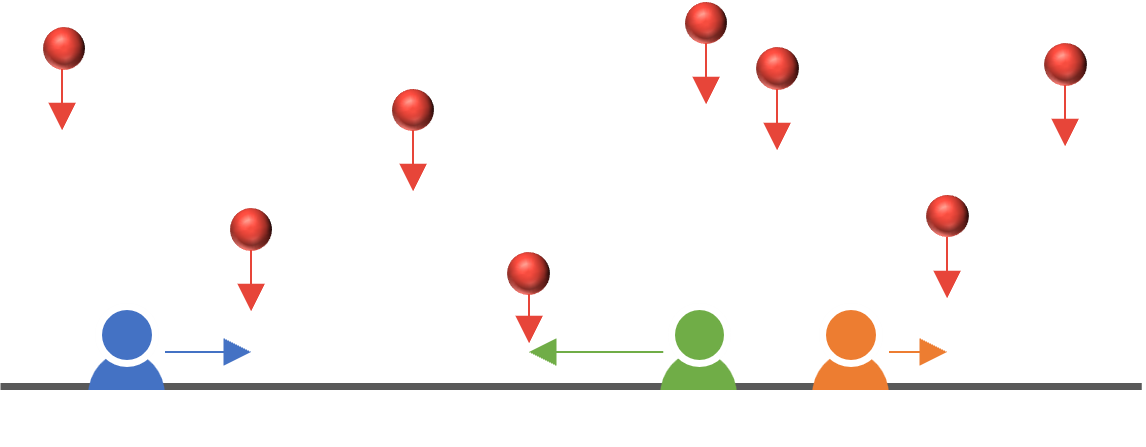
\includegraphics[width=1\linewidth]{chapters/bd/fig/bdhd.png}
    \vspace{-6mm}
    \caption[Illustration of the problem of boundary defense with heterogeneous defenders]
    {Illustration of the problem of boundary defense with heterogeneous defenders, where multiple defenders with different capabilities must do their best to intercept incoming attacks (signified as red balls moving downwards). The defenders are constrained to move on the boundary, which is a 1D perimeter in this case.}
    \label{fig:bd-bdhd}
    \vspace{-5mm}
\end{figure}
% \textbf{Related Work.}

%TODO: we focus on scalability (1) developed ILP algo (2) developed scalable algo (3) these algos enable us to carry out empirical studies including working with multiple topologies (can discuss hardness?)

The main contribution of our work lies in the development of efficient computational tools for and an empirical structural study of \prob. More specifically, 
\begin{itemize}[leftmargin=3.5mm]
\item We developed a network-flow formulation of \prob, leading to an exact method, based on integer linear programming (ILP), for solving the problem. The IP-based method is much more scalable than the DP-based method (which is only effective for no more than three defenders). 
% and the NP-hardness on the flow formulation of the problem  
\item Using the DP solution as a sub-routine, we developed a highly scalable heuristics method, called \emph{exhaustive defender pairing} (\ours), that runs in low polynomial time.  \ours is demonstrated to compute high-quality (in fact, often optimal or near-optimal) solutions. The design philosophy of \ours is of independent algorithmic interest. 
\item We further generalize our algorithms to apply to finite-horizon \prob (more challenging than infinite-horizon \prob), where only attacks whose attack time is within some $T$ time of hitting the boundary are revealed.
\item Utilizing the scalable algorithms developed in this work, we performed a thorough empirical study of the solution characteristics of \prob under various possible problem settings, including (1) different attack densities, (2) different defender speed distributions, and (3) different domain topology, i.e., $S^1$ (circle), $I = [0, 1]$ (unit interval), $S^2$ (sphere), and $I \times I$ (unit square). 
\end{itemize}

%2) a heuristic method based on exhaustive defender pairing that significantly reduces the computation time to solve perimeter defense problem with heterogeneous robot speed in a one-shot setting.
%3) a natural extension of the algorithm for the one-shot setting to the finite horizon continuous setting, where the robot team only know the attack events within a certain time frame in the future.

The rest of the chapter is organized as follows. 
In Sec.~\ref{sec:bd-preliminary}, we formulate the problems studied in this chapter and introduce the notations used. 
In Sec.~\ref{sec:bd-algorithm}, we describe the previous dynamic programming method in \cite{adler2022role}, 
and our ILP-based algorithms and \ours. 
We discuss the performance of our algorithms and solution characteristics of \prob under different settings in 
Sec.~\ref{sec:bd-evaluation}, 
and conclude with Sec.~\ref{sec:bd-conclusion}.
% The papers concludes with 

\label{sec:bd-intro}
\subsection{Preliminaries}\label{sec:bd-preliminary}
In boundary defense with heterogeneous defenders (\prob), there are $k$ defenders (which may be robots and/or other types of agents) with speeds $v_1,\dots,v_k$, where each defender is modeled as a point in some domain $\mathcal E = \mathbb R^2$ or $\mathbb R^3$.
The defenders live on a lower dimensional subspace of $\mathcal E$ (i.e., some boundary of a subset of $\mathcal E$).  
There are also $n$ attack events $\big\langle loc_i, t_i\big\rangle_{i=1}^{n}$, where each attack event is a pair $\big\langle loc, t\big\rangle$ in which $loc$ is the
location of the attack and $t$ is the time it happens. 
The $i^{{th}}$ attack is intercepted by a defender only if the defender is located at $loc_i$ at time $t_i$.
For initialization, we denote the initial locations of the $k$ defenders at $t=0$ as $loc^{1},\dots, loc^{k}$. 

Following the definition in \cite{adler2022role}, we define the horizon of the defenders as follows,
\begin{definition}[Horizon]
The (look ahead) \textit{horizon} $T$ of the defenders is defined as the amount of time defenders can peek into the attack sequence in the future. That is, given the current time $t$, and a horizon $T$, defenders have access to complete information on attacks happening on or before $t+T$. 
\end{definition}

Now, we provide formulations of the two versions of the \prob problem studied in this paper. In the infinite horizon setting, $T = \infty$, all attack events are given in a single batch.

\begin{problem}[Infinite-horizon \prob]\label{prob:bd-1}
Given $k$ defenders with speed $v_1, \dots, v_k$ and initial locations $loc^1, \ldots, loc^k$, and $n$ attack events $\big\langle loc_i, t_i\big\rangle_{i=1}^{n}$, intercept as many attacks as possible. 
\end{problem}

In a finite-horizon setting, the attack events are not all revealed at $t=0$ but are given as a stream of attacks $\big\langle loc_i, t_i\big\rangle_{i=1}^{\infty}$. The defenders can only know the attack events within a horizon or time window of $T < \infty$ in the future.

\begin{problem}[Finite-horizon \prob]\label{prob:bd-2}
There are $k$ defenders with speed $v_1, \dots, v_k$ and initial locations $loc^1, \ldots, loc^k$, and a stream of attack events.
%
At each time instance $t$, the defenders only know attack events happening no later than time $T$ in the future (i.e. $t_i \le t+T$).
%
Intercept as many attacks as possible. 
\end{problem}

We introduce here two useful notations: $next(a, d)\ (a\in[0, n],\ d\in[1,k])$ and $prev(a, d)\ (a\in[1,n],\ d \in [1,k])$.
They are defined as
\begin{align}
next(a, d) = \{ a'| dist(loc_a, loc_{a'}) \leq v_d \cdot (t_{a'} - t_a) \}    \\
prev(a, d) = \{ a'| dist(loc_a, loc_{a'}) \leq v_d \cdot (t_a - t_{a'}) \}    
\end{align}
where $dist(x,y)$ denotes the distance between location $x$ and $y$. 
In other words, $next(a, d)$ is the set of 
attack events that can be reached from the location of the $a^{th}$ attack event by defender $d$. 
And $prev(a,d)$ is the set of attack events from whose location defender $d$ can reach the $a^{th}$ attack event. 
Additionally, $next(0, d)$ denotes the set of attack events that can be reached by defender $d$ from its initial location.
Similarly, $prev(a, d)$ contains $0$ if defender $d$ can reach the location of attack $a$ from its initial location.
~\ref{fig:bd-next_prev} gives an example for defender $1$.

\begin{figure}[h]
    \centering
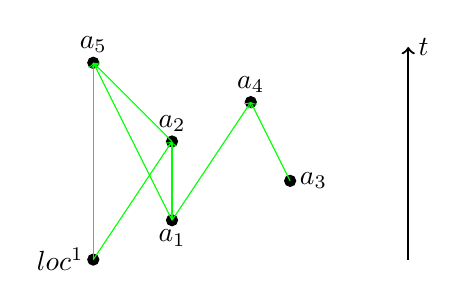
\begin{tikzpicture}
%\draw[black, thick, ->] (0,0) -- (4.5,0) node[anchor=south]{location};
\draw[black, thick, ->] (5,0) -- (5, 2.7) node[anchor=west]{$t$};

\filldraw[black] (1, 0) circle (2pt) node[anchor=east](iloc1){$loc^1$};

\filldraw[black] (2,0.5) circle (2pt) node[anchor=north](a1){$a_1$};
\filldraw[black] (2,1.5) circle (2pt) node[anchor=south](a2){$a_2$};
\filldraw[black] (3.5,1) circle (2pt) node[anchor=west](a3){$a_3$};
\filldraw[black] (3,2) circle (2pt) node[anchor=south](a4){$a_4$};
\filldraw[black] (1,2.5) circle (2pt) node[anchor=south](a5){$a_5$};

\draw[green, thin, ->] (iloc1.east) -- (a2.south);
\draw[green, thin, ->] (iloc1.east) -- (a5.south);

\draw[green, thin, ->] (a1.north) -- (a2.south);
\draw[green, thin, ->] (a1.north) -- (a4.south);
\draw[green, thin, ->] (a1.north) -- (a5.south);
\draw[green, thin, ->] (a2.south) -- (a5.south);
\draw[green, thin, ->] (a3.west) -- (a4.south);

\end{tikzpicture}
    \caption{Illustration of an example of reachability between different attack events for defender $1$.  
    For example, $next(1, 1) = \{2,4,5\}$, $next(0,1)=\{2,5\}$, $prev(2, 1) =\{0, 1\}$, $prev(1,1)=\varnothing$.
    $loc^1$ cannot reach $a_1$ since $v_1$ is not sufficiently large. For the same reason, defender $1$ cannot reach $a_3$ from $a_1$.
    }
    \label{fig:bd-next_prev}
\end{figure}


% 
\section{Structural Analysis}
Given that barrier forming problems studied in this work are NP-hard, a natural algorithmic choice for addressing the challenge is through exploring  mathematical programming.
%
To that end, a model must be built that selects from candidate barriers, which in turn requires the construction of a representative set of barrier candidates, a rather non-trivial task. 
%
The set of candidate barriers should satisfy two conflicting constraints: (1) it should contain a minimum set line segments that achieves the desired separation and (2) its size should not be too big that it will cripple the barrier selection process. 
%
Through careful structural analysis, we notice that the barriers to be considered can be limited to \emph{tangent} or \emph{bitangent} line segments. A tangent line segment, with respect to an object or an obstacle, is a line that passes through a vertex or an edge of the object/obstacle but does not intersect its interior. A bitangent is a line segment that is tangent to two objects and/or obstacles. 
%
This allows us to significantly reduce the number of candidates to be examined at the later selection stage.

\begin{theorem}\label{theorem:sin_tan}
For any $k$ sets of polygonal or point objects $S_1, \dots, S_k$ in the workspace $\mathcal W$, the set of line segments that are tangential to the objects and obstacles contains a set of minimum cardinality that separates $S_1, \dots, S_k$. 
\end{theorem}


\begin{proof}

% We prove that there exists a set of lines with minimum cardinality that separates $S_1, \dots, S_k$, and consists of only lines tangent to object vertices. 
Consider a set of line segments $L^*$ with minimum cardinality that separates $S_1,\dots, S_k$. 
Without loss of generality, we assume all line segments in $L^*$ do not end in the free space, i.e., each line segment in $L^*$ ends
at either object boundaries or workspace boundaries.
If some line segment in a minimum barrier is not tangent to any object vertex, denoted it as $\ell=OA$ (shown in Fig.~\ref{fig:proof}), we show that it can be replaced by a line segment that is tangent to some object vertex. 
%
Fix one end of $\ell$, $O$ in this case, and rotate $\ell$ around $O$ in both clockwise and counterclockwise directions until it hits some object vertex and becomes tangential to the object.
%
Denote the two line segments resulting from clockwise rotation and counterclockwise rotation as $\ell_1'=OB$ and $\ell'_2=OC$, respectively. 

We show $\ell$ can be replaced with $\ell_1'$ or $\ell_2'$. 
If this is not the case,
since replacing $\ell$ with $\ell_1'$ cannot make the separation work, there must be some point $P_1$ between $AB$ that is path connected to some point in the other class without crossing any line segments in $L^*$ when $\ell$ is replaced with $\ell'_1$. Denote the point as $D_1$ and the path as $path_1$. 
The same analysis goes for $\ell'_2$, that if $\ell$ cannot be replaced by $\ell_2$ then there is some point $P_2$ in $AC$ and path $path_2$ that connects $P_2$ to some other point $D_2$ in a different class and crosses segment $\ell$ but not $\ell_2'$. 
Since there are no objects or obstacles inside triangle $OCB$, we can assume the parts of $path_1$ and $path_2$ inside triangle $OCB$ are straight lines.
So, $path_1$ and $path_2$ must cross each other at some point. 
Denote the cross point as $Q\in path_1 \cap path_2$. 
Then, $path_1 = path_{11} (from\ P_1\ to\ Q) + path_{12} (from\ Q\ to\ D_1)$ and $path_2 = path_{12} (from\ P_2\ to\ Q) + path_{22} (from\ Q\ to\ D_2)$. 
Path $p_{11} + p_{22}$ connects $P_1$ to $D_2$, and $p_{21} + p_{12}$ connects $P_2$ to $D_1$, one of which must not cross $\ell$. 
This leads to a contradiction to the fact that the original line set $L^*$ separates the $k$ classes of objects.

Therefore, each non-tangent line segment in $L^*$ can be replaced with a tangent line segment. 
It will eventually result in a set of tangent barriers with minimum cardinality that separates $S_1,\dots,S_k$.
\begin{figure}[ht]
    \vspace{-2mm}
    \centering
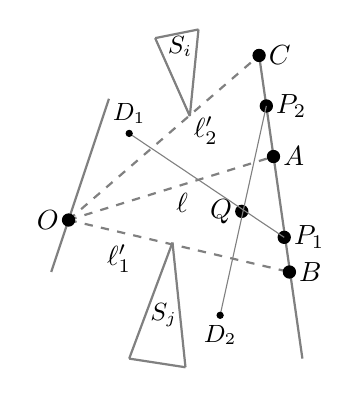
\begin{tikzpicture}[scale = 1.1]
\draw[gray, thick] (0.1, 0) -- (0.7666, 2);
\draw[gray, thick] (3, -1) -- (2.5, 2.5);


\draw[gray, thick] (1, -1) -- (1.5, 0.34);
\draw[gray, thick] (1.65, -1.1) -- (1.5, 0.34);
\draw[gray, thick] (1.65, -1.1) -- (1, -1);

\draw[gray, thick] (1.3, 2.7) -- (1.7, 1.8);
\draw[gray, thick] (1.8, 2.8) -- (1.7, 1.8);
\draw[gray, thick] (1.8, 2.8) -- (1.3, 2.7);

\draw[gray, thick, dashed] (0.3, 0.6) -- (2.66666, 1.333);

\draw[gray, thick, dashed] (0.3, 0.6) -- (2.5, 2.5);
\draw[gray, thick, dashed] (0.3, 0.6) -- (2.85, 0);

\node[text width=1cm] at (2, 0.8) {$\ell$};
\node[text width=1cm] at (2.2, 1.63) {$\ell_2'$};
\node[text width=1cm] at (1.2, 0.15) {$\ell_1'$};

\filldraw[black] (0.3, 0.6) circle (2pt) node[anchor=east] {$O$};
\filldraw[black] (2.666, 1.333) circle (2pt) node[anchor=west] {$A$};
\filldraw[black] (2.5, 2.5) circle (2pt) node[anchor=west] {$C$};
\filldraw[black] (2.85, 0) circle (2pt) node[anchor=west] {$B$};

\filldraw[black] (2.79, 0.4) circle (2pt) node[anchor=west] {$P_1$};
\filldraw[black] (2.5833, 1.917) circle (2pt) node[anchor=west] {$P_2$};

\filldraw[black] (2.3, 0.7) circle (2pt) node[anchor=east] {$Q$};

\draw[gray] (2.79, 0.4) -- (1.0, 1.6);
\draw[gray] (2.5833, 1.917) -- (2.05, -0.5);
\filldraw[black] (1.0, 1.6) circle (1pt) node[anchor=south] {\small{$D_1$}};
\filldraw[black] (2.05, -0.5) circle (1pt) node[anchor=north] {\small $D_2$};


\node[text width=1cm] at (1.9, 2.6) {\small $S_i$};
\node[text width=1cm] at (1.7, -0.5) {\small $S_j$};

\end{tikzpicture}
    \caption{Rotating non-tangent barrier line segment $\ell$ in clockwise and counterclockwise directions around its endpoint $O$ until it becomes tangential to some objects.}
    \label{fig:proof}
    \vspace{-2mm}
\end{figure}
% Then, we show that there exists a set of lines with minimum cardinality that separates $S1$ and $S2$. Similarly, when a line is only tangent to one vertex
\end{proof}

Although we can limit the candidate barriers to line segments tangent to object vertices, there can
still be infinite number of candidates. 
One may consider using line segments that are bitangent to
object vertices, i.e. line segments crossing two object or obstacle vertices. If there are $n$ object/obstacle vertices, there can be at most $n^2$, i.e., a quadratic number of bitangents. 
Unfortunately, bitangent lines are insufficient to act as candidate barriers by themselves for polygonal objects. A counterexample in Fig.~\ref{fig:counter} shows that there is an instance where an optimal solution must contain line segments that are not bitangents. 
%
In this counterexample, we need separate the orange objects from the lime object. A minimum of three line segments are used, and it is not possible that all of them are bitangent, i.e.

\begin{proposition}
Bitangent line segments do not always contain optimal solution for the barrier forming problem for polygonal objects.
\end{proposition}

\begin{figure}[ht]
    \centering
    \vspace{-.2in}
    \includegraphics[width = .25\textwidth]{chapters/bc/fig/counter_example.png}
    \vspace{0.0in}
    \caption{Counterexample that shows using only bitangent line segments cannot create the optimal solution}
    \label{fig:counter}
\end{figure}

Despite the caveat, for the first two formulations that deal with barrier forming for point sets, even with polygonal obstacles, bitangent line segments
always contain an optimal solution. More precisely, 
\begin{theorem}
For any $k$ sets of point objects $S_1, \dots, S_k$ in a workspace $\mathcal W$, there exists
a set of line segments with minimum cardinality that separates $S_1, \dots, S_k$, 
and only consists of bitangent line segments.
\end{theorem}

\begin{proof}
From Theorem~\ref{theorem:sin_tan}, we can see using single tangent line segments is always enough
for an optimal solution. 
Now we turn an optimal solution, $L^*$, with only tangent line segments, into
a solution with only bitangent line segments while still maintaining the same number of barriers. 

For a tangent line segment $\ell=AB\in L^*$ with tangent point $O$ (shown in Fig.~\ref{fig:proof_bi}), and if $O$ is a point object, assume it is beneath $\ell$,
rotate $\ell$ clockwise around $O$ until it hits a point object or an obstacle vertex.
Denote the resulting line segment as $\ell'$, and replace $\ell$ with $\ell'$.
Since the objects are point objects, so $BB'$ and $AA'$ must belong to obstacles or workspace boundary, 
and thus there is no object point inside $OAA'$ or $OBB'$. 
Therefore, the replacement won't result in
any path connecting objects in different classes.
If this is not the case, then there will be some path connecting two object points in different classes that crosses $\ell$ but does not cross $\ell'$ or other barriers. 
Since the triangle areas $OAA'$ and $OBB'$ are empty, that path must enter region $OAA'$ or $OBB'$ and leave them from $\ell$. Then, that part of the path could be replaced with a straight line segment parallel to $\ell$ which prevents it from crossing $\ell$. This contradicts the assumption that $L^*$ prevents all connections between objects in different classes. % of objects.

Continuing the replacement until all line segments are bitangent will result in an optimal solution with only bitangent line segments.

\begin{figure}[ht]
    \centering
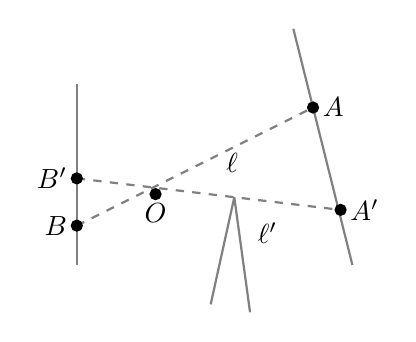
\begin{tikzpicture}
% \draw[gray, thick] (0, 0) -- (1, 2);
\draw[gray, thick] (2.5, -1) -- (1.75, 2);
\draw[gray, thick] (-1, -1) -- (-1, 1.3);

\draw[gray, thick] (0.7, -1.5) -- (1, -0.14);
\draw[gray, thick] (1.2, -1.6) -- (1, -0.14);

% \draw[gray, thick] (3, -1) -- (2.5, 2.5);

% \draw[gray, thick] (1, -1) -- (1.5, 0.34);
% \draw[gray, thick] (1.65, -1.1) -- (1.5, 0.34);
% 
% \draw[gray, thick, dashed] (0.3, 0.6) -- (2.66666, 1.333);
\draw[gray, thick, dashed] (-1., -0.5) -- (2., 1.);

\draw[gray, thick, dashed] (-1., 0.1) -- (2.35, -0.3);

% \draw[gray, thick, dashed] (0.3, 0.6) -- (2.5, 2.5);
% \draw[gray, thick, dashed] (0.3, 0.6) -- (2.85, 0);

\node[text width=1cm] at (1.4, 0.3) 
                        {$\ell$};
% \node[text] at (1.8, 1.63) 
                        % {$\ell_2'$};
\node[text width=1cm] at (1.8, -0.6) 
                        {$\ell'$};

\filldraw[black] (0.0, -0.1) circle (2pt) node[anchor=north] {$O$};
\filldraw[black] (2, 1.) circle (2pt) node[anchor=west] {$A$};
% \filldraw[black] (2.5, 2.5) circle (2pt) node[anchor=west] {$C$};
\filldraw[black] (-1, -0.5) circle (2pt) node[anchor=east] {$B$};

\filldraw[black] (2.35, -0.3) circle (2pt) node[anchor=west] {$A'$};
\filldraw[black] (-1, 0.1) circle (2pt) node[anchor=east] {$B'$};

% \filldraw[black] (2.7583, 0.6666) circle (2pt) node[anchor=west] {$P_1$};
% \filldraw[black] (2.5833, 1.917) circle (2pt) node[anchor=west] {$P_2$};

\end{tikzpicture}
    \caption{Rotating a single tangent barrier line segment $\ell$ around its tangent point $O$ clockwise until it becomes bitangent.}
    \label{fig:proof_bi}
\end{figure}
\end{proof}

For separating polygonal objects, although using bitangent line segments cannot guarantee an optimal solution that uses minimum number of line segments, they can still ensure that solutions limited to bitangents are at least $2$-optimal.
\begin{proposition}
For any $k$ sets of polygonal objects $S_1, \dots, S_k$ in the workspace $\mathcal W$, there exists a set of line segments with cardinality at most twice the minimum cardinality, that separates $S_1, \dots, S_k$, and only consists of line segments that are bitangent to object or obstacle vertices. 
\end{proposition}
\begin{proof}


\begin{figure}[ht]
    \centering
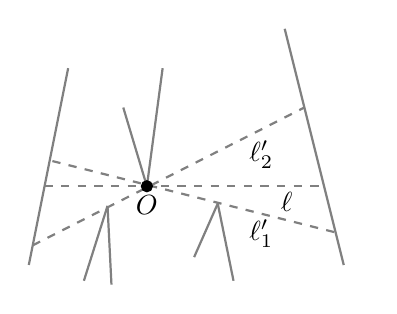
\begin{tikzpicture}

\draw[gray, thick] (2.5, -1) -- (1.75, 2);
\draw[gray, thick] (-1.5, -1) -- (-1, 1.5);
\draw[gray, thick] (0, 0) -- (-0.3, 1);
\draw[gray, thick] (0, 0) -- (.2, 1.5);

\draw[gray, thick] (-0.8, -1.2) -- (-0.5, -0.25);
\draw[gray, thick] (-0.45, -1.25) -- (-0.5, -0.25);

\draw[gray, thick] (0.6, -0.9) -- (0.9, -0.22);
\draw[gray, thick] (1.1, -1.2) -- (0.9, -0.22);


\draw[gray, thick, dashed] (-1.45, -0.75) -- (2., 1.);
\draw[gray, thick, dashed] (-1.3, -0.0) -- (2.2, 0);

\draw[gray, thick, dashed] (-1.2, 0.32) -- (2.45, -0.6);



\node[text width=1cm] at (2.2, -0.2) 
                        {$\ell$};

\node[text width=1cm] at (1.8, -0.6) 
                        {$\ell'_1$};

\node[text width=1cm] at (1.8, 0.4) 
                        {$\ell'_2$};

\filldraw[black] (0.0, -0.0) circle (2pt) node[anchor=north] {$O$};


\end{tikzpicture}
    \caption{Rotating tangent barrier line segment $\ell$ both clockwise and counterclockwise around its tangent point $O$ until it becomes bitangent.}
    \label{fig:proof_bi_2opt}
\end{figure}

Starting from an optimal solution $L^*$ with only tangent line segments,
we will replace each tangent line segment with two bitangent line segments.

Rotate each non-bitangent line segment $\ell\in L^*$ around its tangent point $O$ in clockwise or counterclockwise directions until the line segment become bitangent, as illustrated in Fig.~\ref{fig:proof_bi_2opt}. 
Since any path connecting two objects in different classes and is cut by barrier $\ell$ will still be cut by $\ell'_1$ and $\ell'_2$.
The replacement can still guarantee the separation among the object groups.
After replacing all barriers, we can obtain a 2-OPT solution with the number of line segments twice the minimum.
\end{proof}
\label{sec:bd-structure}
\subsection{Algorithmic Solutions for \prob}\label{sec:bd-algorithm}
In this section, we describe three methods for solving infinite-horizon \prob (Problem~\ref{prob:bd-1}).
Sec.~\ref{sec:bd-dp} provide a dynamic programming (DP) algorithm based on one developed in \cite{adler2022role}, 
followed by Sec.~\ref{sec:bd-ilp} formulating an integer linear programming model,
and Sec.~\ref{sec:bd-dp_local} discusses a heuristic search algorithm based on the DP algorithm. 
The extension to an infinite attack stream with a finite look-ahead horizon  (Problem~\ref{prob:bd-2}) will be discussed in Sec.~\ref{sec:bd-hor}.


\subsection{Exact Dynamic Programming Based Method}%for A Fixed Number of Defenders}
\label{sec:bd-dp}

The DP algorithm builds a recursion formula on the last attacks intercepted by the defenders.
Without loss of generality, we assume that each attack is only intercepted by one defender.
For a DP state $a_1, \dots, a_k$ where $a_i$ is the last attack defender $i$ intercepts, 
let $T[a_1]\dots[a_k]$ store the maximum number of attacks that can be intercepted when the $i^{th}$ defender's last intercepted attack events is $a_i$ $(i\in[1,k])$,
and denote $a_{ma}$ as the maximum of $a_1, \dots, a_k$.
Base on which attack the $ma^{th}$ defender intercepts before intercepting attack $a_{ma}$,
we can write the DP recursion formula as follows.
\begin{equation}
\begin{split}
T[a_1]\dots[a_{ma}]\dots[a_k] &= \\ 
\max_{p\in prev(a_{ma}, ma) \wedge p\neq a_1 \dots a_k} &  T[a_1]\dots[p]\dots[a_k] + 1
\end{split}
\end{equation}

Pseudo-code in Alg.~\ref{alg:bd-dp} provides a sketch of a possible implementation of the dynamic programming algorithm.
Effectively implemented, the time complexity of running Alg.~\ref{alg:bd-dp} is $O( (n+1)^{k+1})$, which is polynomial when $k$, the number of defenders, is fixed.
\vspace{-2mm}

\begin{algorithm}
%\begin{small}
\DontPrintSemicolon
\KwData{
$E=\big \langle loc_i, t_i\big\rangle_{i=1}^{n}$: $n$ attack events\;
$loc^1,\dots,loc^k$: initial locations of the $k$ defenders\;
$v_1,\dots,v_k$: speeds of the $k$ defenders\;
}
\KwResult{Maximum number of attacks intercepted}
\vspace{1mm}
$T\gets$ an $(n+1)^k$-length array initialized to $-\infty$\;
\vspace{1mm}
$result\gets 0$\;
\vspace{1mm}
$T[0]\gets 0$\;
\vspace{1mm}
\For{$mask\gets 0 $ \KwTo $(n+1)^k - 1$}{
\vspace{1mm}
    $\overline{a_1 a_2\dots a_k} \leftarrow mask$\;
    \Comment{$\overline{a_1 a_2\dots a_k}$ represents a base-($n+1$) number, i.e., $a_1\cdot (n+1)^{k-1} + a_2 \cdot (n+1)^{k-2} +\dots+ a_k$}
    \If{$\exists\ a_i = a_j$}{
        \Continue\;
    }
\vspace{1mm}
    $ma \leftarrow argmax_i a_i$\;
\vspace{1mm}
    \For{$p\in prev(a_{ma}, ma)$}{
        \If{$\forall i\ pos_i \neq p$}{
            $pm\gets mask - (a_{ma} - p)\cdot (n+1)^{k-ma}$\;
            \Comment{$pm$ is the result of replacing $a_{ma}$ with $p$}
            $T[mask]\gets \max(T[mask], T[pm] + 1)$\;
        }
    }
\vspace{1mm}
    $result\gets \max(result, T[mask])$\;
}
\vspace{1mm}
\Return{$result$}\;

\caption{Dynamic Programming for \prob}
\label{alg:bd-dp}
%\end{small}
\end{algorithm}
\vspace{-2mm}
%\vspace{-15mm}

The algorithm presented here is a slight modification of the DP algorithm in \cite{adler2022role} with two subtle differences. First, we enforce that an attack event can only be handled by one defender.
Second, we explicitly use the initial locations of the defenders in the algorithm, which is essential for handling the finite horizon extension.

\subsection{Solving \prob with Integer Linear Programming Model based on a Flow Formulation}
\label{sec:bd-ilp}

It is not difficult to see that \prob can also be seen as a network flow problem by treating each attack event as a node and the reachability between each pair of attack events for each defender as the edges in the graph. 

Specifically, there are $n$ nodes in the graph, representing the $n$ attack events. 
There are also $O(n^2k)$ connections between nodes inside the graph.
If defender $j$ can reach attack event $i'$ from $i$, there is an connection 
$edge[i][i'][j]$ between node $i$ and $i'$. 
Also, we use a binary variable $intercept[i]$ to denote whether attack event $i$ is successfully intercepted. 
These give rise to the following integer linear programming (ILP) formulation of the problem.

% \begin{gather}
Eq. \eqref{eq:bd-intercept} sets the criteria of an attack $i$ being intercepted as at least one defender to come into the node $i$, which means intercept attack $i$.
Eq. \eqref{eq:bd-flow} sets the defender flow conservation rule that the number of type $j$ defender exiting node $i$ must be larger than or equal to the number of type $j$ defender coming to node $i$.
Eq. \eqref{eq:bd-initial} sets the initial constraints on the number of each type of defender used (coming out from node 0).

\begin{gather}
\sum_{j\in[1, k],\ i'\in prev(i, j)} edge[i'][i][j] \geq intercept[i] \label{eq:bd-intercept}\\
\sum_{nxt_i\in next(i, j)} edge[i][nxt_i][j] \leq \sum_{prv_i \in prev(i,j)} edge[prv_i][i][j]  \label{eq:bd-flow} \\
\sum_{nxt_0 \in next(0, j)} edge[0[nxt_0][j] \leq 1 \label{eq:bd-initial}  \\
Objective\quad \max \sum_i intercept[i]
\end{gather}

% \end{gather}
Denote $M$ as the number of connections in the graph, clearly $M<n^2k$.
This integer linear programming formulation uses $M + n$ variables, and 
$nk + n$ constraints. 

%It may not be worth mentioning
\begin{remark}
The flow formulation of the problem is an NP-hard problem. The proof is similar to the NP-completeness proof of the two-commodity flow in \cite{even1975complexity}. This seems to suggest that \prob is NP-hard as well. 
\end{remark}

% \begin{proof}
% \end{proof}

\subsection{Exhaustive Defenders Pairing Heuristic Search Method}
\label{sec:bd-dp_local}
We now develop a heuristic search method using the dynamic programming algorithm discussed in Alg.~\ref{alg:bd-dp} 
applied on two defenders.
The DP algorithm that computes the optimal solution for two defenders is used as a local improvement primitive 
for the local search heuristic algorithm. 

We call the resulting algorithm \emph{exhaustive defender pairing} (\ours).  
In each iteration, \ours pick two defenders, and the attack events the two defenders have intercepted and the attack events that have not been intercepted by any defender. 
Then, \ours uses the DP algorithm in Alg.~\ref{alg:bd-dp} to increase the number of attack events intercepted by the two defenders selected. 
The complete algorithm is sketched in Alg.~\ref{alg:bd-dp_local}.

\begin{algorithm}[h]
\DontPrintSemicolon
\KwData{
$E=\big \langle loc_i, t_i\big\rangle_{i=1}^{n}$: $n$ attack events\;
$loc^1,\dots,loc^k$: initial locations of the $k$ defenders\;
$v_1,\dots,v_k$: speeds of the $k$ defenders\;
}
\KwResult{Number of attacks intercepted}

$Intercept \gets$ a length-$n$ array initialized to $-1$\;
\Comment{$Intercept$ array stores for each event the defender that intercepts it}
$result\gets 0$\;
\vspace{1mm}
\For{$u, v \in \{1, \dots, k\}\times\{1, \dots, k\}, u\neq v$}{
    $E'\gets \{w\ |\ Intercept[w] \in\{u, v, -1\}\}$ \;
    \Comment{$E'$ stores the set of attack events intercepted by defender $u,v$ and the attacks not intercepted by any defender}
\vspace{1mm}
    $\tilde{n}\gets E'.size$\;
\vspace{1mm}
    T $\gets$ an $(\tilde{n}+1)^2$-length array initialized to $-\infty$\;
\vspace{1mm}
    $T[0]\gets 0$\;
    \Comment{Apply the DP algorithm for defender $u$ and $v$}
\vspace{1mm}
    \For{$mask\gets 0 $ \KwTo $(\tilde{n}+1)^2-1$}{
        $\overline{a_1 a_2} \leftarrow mask$\;
        \If{$a_1 =a_2$}{
            \Continue\;
        }
\vspace{1mm}
        $ma \leftarrow argmax_i a_i$\;
\vspace{1mm}
        \For{$p\in prev(a_{ma}, ma)$}{
            \If{$\forall i\ a_i \neq p$}{
                $pm\gets mask - (a_{ma} - p)\cdot (n+1)^{2-ma}$\;
                $T[mask]\gets \max(T[mask], T[pm] + 1)$\;
            }
        }
        % $result\gets \max(result, T[mask])$\;
    }
\vspace{1mm}
    \If{Solution is improved}{
        Update $Intercept, result$\;
    }
}
\vspace{1mm}
\Return{$result$}
\caption{Exhaustive Defender Pairing}
\label{alg:bd-dp_local}
\end{algorithm}

We can try different defender pairing orders and choose the best one. 
In our \ours implementation, we choose to run line 3 of Alg.~\ref{alg:bd-dp_local} in 3 different iteration ordering of $u, v$.
Alg.~\ref{alg:bd-dp_local}'s running time is $O(k^2 n^3)$ as we try $O(k^2)$ pairs of defenders, and each run of the DP algorithm takes $O(n^3)$.
% ($u$ increasing from $1$ to $k$, decreasing from $k$ to $1$, increasing from $k/2$ to $k$ after which go back to $1$ and increase to $k/2-1$). 

\subsection{Handling Infinite Attack Streams with a Finite Look-Ahead Horizon }
\label{sec:bd-hor}
For Problem~\ref{prob:bd-2} where the attacks $\big \langle loc_i, t_i\big \rangle_{i=1}^{\infty}$ may be infinite, and the look-ahead horizon is finite, not all attacks are revealed at once. As such, previous methods cannot be directly applied. 
As the future attack sequence cannot be foreseen, defenders need to \emph{react} to information (e.g., the attack events in the next $T$ time interval) obtained so far. 

Towards addressing the problem, a greedy \emph{replanning} approach can be applied. Whenever an attack event is observed, the defender team replans the capture sequence given the new attacks added to the attack queue. 
This gives rise to an online algorithm sketched in Alg.~\ref{alg:bd-horizon}.

\begin{algorithm}[h]
\DontPrintSemicolon
\KwData{
$E=\big \langle loc_i, t_i\big\rangle_{i=1}^{\infty}$: a stream of attack events\;
$loc^1,\dots,loc^k$: initial locations of the $k$ defenders\;
$v_1,\dots,v_k$: speeds of the $k$ defenders\;
}
$E'\gets $ an empty queue\;
\Comment{$E'$ stores attack events seen so far}
\vspace{1mm}
\While{new attack events added to $E'$ }{
    Apply Alg.~\ref{alg:bd-dp_local} to compute a plan for the defenders and attack events $E'$\;
    Execute the plan, pop out from $E'$ attack events passed, and update $loc^1,\dots,loc^k$ to the defenders' current locations until new attacks are foreseen\;
}
% \KwResult{Number of attacks intercepted}

% $Intercept \gets$ a length-$n$ array initialized to $-1$\;
% \Comment{$Intercept$ array stores for each event the defender that intercepts it}
% $result\gets 0$\;
% \For{$u, v \in \{1, \dots, k\}\times\{1, \dots, k\}, u\neq v$}{
%     $E'\gets \{w\ |\ Intercept[w] \in\{u, v, -1\}\}$ \;
%     \Comment{$E'$ stores the set of attack events intercepted by defender $u,v$ and the attacks not intercepted by any defender}
%     $\tilde{n}\gets E'.size$\;
%     T $\gets$ an $(\tilde{n}+1)^2$-length array initialized to $-\infty$\;
%     $T[0]\gets 0$\;
%     \For{$mask\gets 0 $ \KwTo $(\tilde{n}+1)^2-1$}{
%         $\overline{a_1 a_2} \leftarrow mask$\;
%         \If{$pos_0 = pos_1$}{
%             \Continue\;
%         }
%         $ma \leftarrow argmax_i pos_i$\;
%         \For{$p\in prev(a_{ma}, ma)$}{
%             \If{$\forall i\ pos_i \neq p$}{
%                 $T[mask]\gets \max(T[mask], 1 + T[\overline{a_1\dots p \dots a_k}])$\;
%             }
%         }
%         % $result\gets \max(result, T[mask])$\;
%     }
%     \If{Solution is improved}{
%         Update $Intercept, result$\;
%     }
% }
% \Return{$result$}
\caption{Online Exhaustive Defender Pairing}
\label{alg:bd-horizon}
\end{algorithm}
\subsection{Evaluation and Empirical Study of \prob}\label{sec:bd-evaluation}
In this section, we describe our experimental study of the methods mentioned or proposed in the paper, which serves two purposes: (1) demonstrating the performance of our fast computational methods, and (2) characterizing the solution structure of \prob under different problem settings.
%

The algorithms are implemented in C++ and run on a 3.6GHz quad-core CPU with 16G memory.
For integer linear programming, Gurobi \cite{optimization2019gurobi} is used as the solver with a time limit of 60 seconds applied.
In the evaluation, two main factors are considered: computation time and solution quality measured by interception rate. 

The instances were generated for up to dozens of defenders, 
and the defender speeds are sampled uniformly at random from $1$ to $v_{max}$.
The attack sequence was generated according to a Poisson process with parameter $\lambda$ (i.e., the time gap between
two consecutive attacks conforms with an exponential distribution $P(t) = \lambda e^{-\lambda t}$),
and the locations of the attack are sampled uniformly at random from the boundary.
We use 4 types of boundary for testing a) unit circle $S^1$, b) unit interval $I=[0, 1]$
c) unit square $I^2=[0, 1]\times[0,1]$, and d) unit sphere $S^2$.

\subsection{Infinite-Horizon \prob: Basic Performance Evaluation}
This section provides experimental study and comparisons between the three methods described in the paper: 
dynamic programming (DP), integer linear programming (ILP), and exhaustive defender pairing (\ours) algorithms.
% \subsubsection{Computation time}

To test and compare the general performance of these methods, we set the defending task on $S^1$ (i.e., a circular boundary with a distance of $2\pi$) 
with the attack sequence's coming rate $\lambda$ (used in the Poisson process) proportional to $k$, the number of defenders. 
The results on computational time and interception rate are given in Figs.~\ref{fig:bd-time_cost} and~\ref{fig:bd-quality}.

\begin{figure}[h!]
    \centering
    \includegraphics[width=.5\linewidth]{chapters/bd/fig/timecost-v.png}
    \caption[Computation time for DP, ILP and \our]{Computation time in seconds ($y$-axis) for dynamic programming (DP), integer linear programming (ILP) and \ours for 2 to 7 defenders and up to 400 attack events ($x$-axis). DP quickly becomes intractable as the number of defenders goes beyond $3$; ILP is about 2-3 magnitudes slower than \ours.}
    \label{fig:bd-time_cost}
\end{figure}

% \subsubsection{Solution quality}

\begin{figure}[h!]
    \centering
    \includegraphics[width=.5\linewidth]{chapters/bd/fig/quality-v.png}
    \caption[Solution quality for DP, ILP and \our]{Solution quality (interception rate) for dynamic programming (DP), integer linear programming (ILP) and \ours  for 2 to 7 defenders. For all settings, \ours achieves optimality nearly identical to the optimal DP and ILP (when DP and ILP can complete the computation). ILP starts to fail as the number of defenders reaches $5$ and the number of events exceeds $300$.}
    \label{fig:bd-quality}
\end{figure}

For 2 to 7 defenders, in ~\ref{fig:bd-time_cost}, we show the computation time of running the algorithms. 
Each data point is an average of 20 runs. 
We remind the readers that both DP and ILP guarantee to produce an optimal solution (if they can finish).
For the two-defender scenario, which is the main focus of \cite{adler2022role}, DP is the most efficient.
However, DP only fully scales for $k=2, 3$ defenders, and start to peter out for $k=4$ defenders due to memory limit (so its running time is not shown for $k>4$).
%The integer programming method was set a time limit of 60s for solving the model.
As can be observed, ILP demonstrates much better scalability in comparison to DP, but fails to find a solution for $k > 5$ defenders. 

As expected, exhaustive defender pairing (\ours) has the least time cost for $k \geq 3$.
~\ref{fig:bd-quality} shows the corresponding solution qualities of these methods. 
We observe that, while \ours does not guarantee solution optimality, it generated solutions that are virtually the same as the exact methods (DP and ILP). 
%
Through these empirical evaluations, \ours demonstrates superior scalability with negligible solution optimality loss. 

%\textbf{JJ's edit location}


\subsection{Scaling up the Number of Defenders}
The number of defenders appears in the index term of the time complexity of the DP algorithm, which limits it from scaling up the number of defenders. Hence, we compare the performance of ILP and the local search algorithm when pushing the number of defenders up to dozens. With the main goal being the evaluation of optimality, we limit the attack events to $200$ so that the ILP method can return the optimal solution in $60$ seconds. At the same time, to make the problem more challenging, 
$\lambda$ is increased to $2\cdot k$ from $k$ so that not all attacks can be intercepted. 
~\ref{fig:bd-def_time_cost} and  ~\ref{fig:bd-def_quality} show the corresponding computation time 
and interception rate, each data point is the average of 20 runs.

\begin{figure}[h!]
    \centering
    \includegraphics[width=.5\linewidth]{chapters/bd/fig/def_timecost-v.png}
    \caption[Computation time in seconds for ILP and EDP algorithms]{Computation time in seconds for ILP and EDP algorithms for $5$ to $30$ defenders and up to $200$ 
    attack events (Limit the number of events because as shown in ~\ref{fig:bd-time_cost}, 
    more events will effectively cripple ILP). \ours consistently demonstrates 1-2 magnitudes faster computation time compared with ILP.}
    \label{fig:bd-def_time_cost}
\end{figure}

\begin{figure}[h!]
    \centering
    \includegraphics[width=.5\linewidth]{chapters/bd/fig/def_quality-v.png}
    \caption[Solution quality (interception rate) for the ILP and EDP]{Solution quality (interception rate) for the ILP and EDP for 5 to 30 defenders. 
    It is straightforward to observe that \ours achieves defending quality nearly identical to the optimal ILP solution (while ILP is still scalable).}
    \label{fig:bd-def_quality}
\end{figure}

As can be observed, EDP, due to its quadratic dependence on the number of defenders, consistently and significantly outperforms the ILP method in terms of computation time. At the same time, it yields virtually the same level of optimality as ILP, which guarantees that the result is optimal. 

\subsection{Impact of Defender Heterogeneity}
To explore the impact of the diversity of defender speeds on interception rate, we focus on a $5$-defender setting and to make the difference more visible, 
$\lambda$ is set to be $5\cdot k = 25$ so that the interception rate no more than 80\%. 
Here, the defender speed diversity is tested by setting the $v_{min}$ as 1, and $v_{max}$ from 1 (uniform speed) to 10, 
and then normalizing the defender speed to make them sum up to $15$ (i.e., with an average of $3.0$). 
Each data point is based on 100 runs. The result is summarized in ~\ref{fig:bd-heterogeneity}, 
from which we can observe that uniform speed $v_{max} = 1$ has the least interception rate, 
while the interception rate gets into its maximum after $v_{max}:v_{min} = 3$ or $4$. 
This suggests that heterogeneity can significantly enhance the interception rate, 
warrant the effort going into the current study (and previous study of heterogeneous defender setups). 
At the same time, as heterogeneity continues to increase, the effect becomes negligible. 
This also follows intuition: when the capability of the defenders varies too much, 
they can no longer effectively collaboratively intercept attacks. 

\begin{figure}[h!]
    \centering
    \includegraphics[width=0.5\linewidth]{chapters/bd/fig/heterogeneity.pdf}
    \caption[Solution quality (interception rate) for a different level of defender speeds diversity]{Solution quality (interception rate) for a different level of defender speeds diversity. It can be observed that the major difference happens as $v_{max}:v_{min}$ increases from $1$ to up to $4$. After that, the increase of interception rate no longer shows improvements.}
    \label{fig:bd-heterogeneity}
    \vspace{-2mm}
\end{figure}

\subsection{Impact of Attack Rate $\lambda$}
With the increase of $\lambda$ in the Poisson process for the attack sequence, 
there will be fewer attacks intercepted, 
and more defenders will be required to reach the same interception rate. 
In this regard, we test the interception rate computed using \ours for $1$ to $20$ defenders and different $\lambda$ from $1.0$ to $60.0$. 
The number of attacks is set to be $400$, and each data point represents an average of 20 runs.
~\ref{fig:bd-lambda} shows the resulting capture rate with respect to the attack rate $\lambda$ as a heat map for a different number of defenders $k$, which, unsurprisingly, suggests a gradual change as one might expect. Nevertheless, such a graph can serve as a quick reference for selecting an appropriate number defenders given an expected attack rate.

\begin{figure}[h!]
    \vspace{-2mm}
    \centering
    \includegraphics[width=0.5\linewidth]{chapters/bd/fig/lambda.pdf}
    \vspace{-2mm}
    \caption[Interception rate with different $\lambda$ (x-axis) and number of defenders]
    {Interception rate with different $\lambda$ (x-axis) and $k$ (y-axis, number of defenders). As one might expect, as attacks happens more frequently, holding other factors unchanged, the interception rate decreases. Similarly, holding other factors unchanged, increasing the number of defenders leads to increased interception rates.}
    \label{fig:bd-lambda}
    \vspace{-2mm}
\end{figure}

\subsection{Impact of Boundary Topology}
\ours applies to \prob with arbitrary boundary topology; we evaluated \ours on $I=[0, 1]$ (unit interval), $S^1$ (circle with a total circumference shrinked to $1$), $I^2$ (unit square), and $S^2$ (sphere with surface area of $1$) (see ~\ref{fig:bd-topology}) with $k = 5$, $v_{max} = 5$ and $\lambda$ from 1 to 200. 
The results are shown in ~\ref{fig:bd-geo}, where each data point is the average of 20 runs. 
We observe that $I$ and $S^1$ have similar difficulty to defend, with $I$ being a bit more challenging due to having boundaries. The same is observed for $I^2$ and $S^2$.
\begin{figure}[h!]
\vspace{2mm}
    \centering
    \includegraphics[width=.5\linewidth]{chapters/bd/fig/topology.png}
    \caption[\prob with boundary topologies $I$ (line segment), $S^1$ (circle), $I^2$ (unit square) and $S^2$ (sphere)]
    {\prob with boundary topologies $I$ (line segment), $S^1$ (circle), $I^2$ (unit square) and $S^2$ (sphere). The red arrows illustrate attack directions. The pictures are captured from animations of actual simulations, available at \url{https://youtu.be/x0mQD\_7RhKI}.}
    \label{fig:bd-topology}
    \vspace{-4mm}
\end{figure}

\begin{figure}[h!]
\vspace{1mm}
    \centering
    \includegraphics[width=.8\linewidth]{chapters/bd/fig/geo.png}
    \caption{Interception rate for $I$, $S^1 (\text{with length 1})$, $I^2$, $S^2 (\text{with surface area 1})$
     with different $\lambda$ from $1$ to $200$. Degradation as the number of attacks increases is as expected.}
    \label{fig:bd-geo}
\end{figure}

\subsection{Infinite Attack Stream with Finite Look-Ahead Horizon}
~\ref{alg:bd-horizon} describes an online \ours algorithm for handling the finite horizon version of the problem where the defenders only have the information about attacks in the next $T$ time frame.
Here, we present some simulation studies using the 5-defender and 400 attacks setup on an $S^1$ boundary with $v_{max} = 5$. 
~\ref{fig:bd-horizon} gives the interception rate with respect to varying defender horizons. Each data point is an average of 20 runs. 
The interception rate converges to around $1$ with a fairly short horizon, 
indicating that a long look-ahead horizon may not be necessary for effectively intercepting attacks.
\begin{figure}
    \vspace{-1mm}
    \centering
    \includegraphics[width=0.6\linewidth]{chapters/bd/fig/horizon.pdf}
    \vspace{-2mm}
    \caption[Interception rate with respect to different horizons]{Interception rate with respect to different horizons (logarithmic scale). It can be observed that longer horizon allows better planning.}
    \label{fig:bd-horizon}
    \vspace{-3mm}
\end{figure}

Lastly, in ~\ref{fig:bd-solution_examples}, we provide the interception trajectories of a typical run for ILP,  \ours, and online \ours. 
%We see that, somewhat interestingly, defender switching does not happen very frequently. 
% I think the term "switching" is a bit misleading
\begin{figure}[h!]
    \vspace{1mm}
    \centering
    \includegraphics[width=.5\linewidth]{chapters/bd/fig/ilp_example-v.png}
    \includegraphics[width=.5\linewidth]{chapters/bd/fig/ls_example-v.png}
    \includegraphics[width=.5\linewidth]{chapters/bd/fig/inf_horizon_example-v.png}
    \caption[The results computed by ILP, \ours, and online \ours]
    {The results computed by ILP, \ours, and online \ours with a horizon of 60, for a sequence of 140 attacks ($x$-axis is the location, $y$-axis is the time of attacks). 
    The number of captured attack events is 71, 70, and 67, respectively.}
    \label{fig:bd-solution_examples}
    \vspace{-4mm}
\end{figure}

\subsection{Conclusion}\label{sec:bd-conclusion}
This paper studied the heterogeneous perimeter defense problem, as formulated in \cite{adler2022role}, with the aim of
significantly boosting the scalability to work on many defenders while achieving high levels of solution optimality.
Toward achieving this goal, we developed an exact integer programming-based algorithm with better scalability than the original dynamic programming (DP) based algorithm from \cite{adler2022role}. We then further developed a fast and highly-effective heuristic based on the pairwise application of DP for computing near-optimal solutions, scaling to dozens of defenders.
%
This pairwise application of DP is of independent algorithmic interest. 
%
In addition, we extend our solution to a more realistic online version in which only attackers within a finite time window are visible. 
%
The algorithms are thoroughly evaluated on a diverse set of boundary topologies including circles, intervals, spheres, and squares. 
%
The evaluation not only confirms that \ours is highly effective but clearly demonstrates the benefit of employing heterogeneous defenders. 


\section{Sweep Line Coverage}
\subsection{Introduction}

Searching for a static or moving target in a planar environment is a classic 
problem in robotics \cite{guibas1999visibility, suzuki1992searching, lavalle2000algorithm, stiffler2017persistent, kolling2007graph}. 
%
The setting applies to many real-world applications, including searching for
lost person/object, checking for potential hazards, and generally, search and rescue tasks conducted in a known environment. 
%
Research tackling this problem mostly focuses on devising a search plan with
different types of objectives, such as minimizing the total length of the
frontier of the search schedule from the start to the end 
\cite{kolling2017coordinated}, minimizing the number of robots used for 
the search plan in a visibility-based robot sensing model
\cite{megiddo1988complexity}, and so on.

In certain cases, the high-level plan for searching a given region may already be pre-determined and fixed. For example, in search and rescue efforts, a frequently carried out plan is to perform a single sweep of an environment with a marching frontier, which is easy to execute when many participating robots/agents are involved.
%
The high-level search plan may also be determined by existing algorithms that 
compute only the search frontier.
%
However, even in the case where the search plan consists of pre-determined 
sweep (frontier) lines; it remains non-trivial to find an optimal organization 
of the mobile robots to execute the search plan, for either minimizing the 
number of robots needed for a given sensing probability requirement or utilizing 
a fixed number of robots to maximize the minimum sensing probability of locating something in the environment. 

\begin{figure}[t]
\vspace{1.5mm}
    \centering

    \begin{subfigure}[t]{0.7\textwidth}
         \centering
        % \vspace{2.5mm}
         \includegraphics[width=\textwidth]{chapters/sc/fig/instance_2.eps}
        %  \vspace{0.5mm}
         \caption{Optimal robot allocations in a vertical sweep}
         \label{fig:sc-vertical}
     \end{subfigure}
    
    %\includegraphics[width=.475\textwidth]{fig/instance_2.eps}
    \medskip
    
    \begin{subfigure}[t]{0.4\textwidth}
         \centering
        % \vspace{2.5mm}
         \includegraphics[width=\textwidth]{chapters/sc/fig/vertical.eps}
        %  \vspace{0.5mm}
         \caption{Vertical}
         \label{fig:sc-vertical}
     \end{subfigure}
    \begin{subfigure}[t]{0.2\textwidth}
         \centering
         \includegraphics[width=\textwidth]{chapters/sc/fig/circular.eps}
         \caption{Circular}
         \label{fig:sc-radial}
     \end{subfigure}
    \begin{subfigure}[t]{0.2\textwidth}
         \centering
         \includegraphics[width=\textwidth]{chapters/sc/fig/rotational.eps}
         \caption{Radial}
         \label{fig:sc-circular}
    \end{subfigure}
     
    \vspace{2mm}
    \caption{(a) An illustration of robots' locations along a left-to-right 
    vertical sweep schedule. Four robots are allocated to execute the vertical sweep, 
    and their trajectories are illustrated in different colors. 
    %
    % There exist discontinuities (jumps) along the trajectories when obstacle vertices 
    % intersect the sweep line, induced by topological changes of the environment. 
    (b)(c)(d) Illustrations of three use cases: vertical, circular, 
    and radial sweeps.}
    \label{fig:sc-sweep}
\end{figure}

In this work, we address the challenge of how to best allocate 
many robots to execute a pre-determined search schedule for a known environment. 
More specifically, for a two-dimensional closed and bounded workspace, and a known 
search schedule, which gives a search frontier for any given time, the robot guards 
are required to stay on the search frontier to carry out the sensing task. 
%
Because each robot's coverage quality deteriorates with distance, their relative 
placement on the frontier must be carefully decided to maximize the coverage quality. 
%
For the setup, we focus on the problem of finding the minimum number of robots required 
to execute a pre-determined sweep schedule such that a minimum sensing quality is 
guaranteed for each point in the workspace. Solutions to this minimization problem 
readily translate to solutions for maximizing the coverage quality for a fixed number 
of robots, which is a dual problem. 

In summary, the main contributions of this work are twofold. First, we generalize the 
notion of boustrophedon decomposition \cite{choset2000coverage}, which partitions the 
plane via vertical sweep, into a decomposition of the plane with a \emph{continuous 
monotone sweep schedule}, which we prove can always be represented as a directed 
acyclic graph (DAG). 
%
Then, we show the problem of minimizing the number of line guards required to execute a sweep schedule can be transformed into a network flow problem.
%
Since the generalized boustrophedon decomposition and the network flow problem can 
be solved in low polynomial time; our method achieves high levels of scalability.
%
The strengths of our method are further corroborated in extensive simulation experiments 
on three realistic use cases: \emph{vertical sweep}, \emph{circular sweep}, and 
\emph{radial sweep} (see, e.g., ~\ref{fig:sc-sweep} (b)(c)(d)).





\noindent
\textbf{Related Work.}
The study in this paper draws inspiration from the study of several 
lines of related problems. 
The Graph-Clear problem, formulated in \cite{kolling2007graph}, tasks a group of robots to search and clear an environment with the operations of blocking and clearing.
A follow-up work on Line-Clear \cite{kolling2017coordinated} uses line guards
with more focus on computational geometry in that
the objective is to minimize the maximum sweep line distance. Both of these problems are
NP-hard, establishing the difficulties of finding a sweep schedule for a planar environment.
The more general pursuit-evasion problem dates back to the research on \emph{search number}
on a discrete graph \cite{megiddo1988complexity}, 
followed by studies on pursuit and evasion continuous environment with 
visibility-based model \cite{guibas1999visibility, suzuki1992searching, lavalle2000algorithm, stiffler2017persistent}. 
The problem becomes the well-known art-gallery problem \cite{o1987art} when a static deployment of robots is sought after.
%
When working with known patrolling search frontiers, e.g., vertical sweep lines, 
this problem is analogous to the perimeter defense problem by placing guards on a static perimeter
to defend intruders \cite{shishika2020cooperative, macharet2020adaptive, chen2021optimal}.
Previously, we have also studied a version of static range guard placement problems for securing perimeters and regions \cite{fengyu2020optimally}.
In contrast to the pursuit-evasion algorithms that deal with searching dynamic and unpredictable targets that could escape, 
coverage planning/control-related algorithms become more suitable for searching or covering predictable or stationary targets,
e.g., room sweeping, pesticide and fertilizer spraying, persistent monitoring, and so on \cite{cortes2004coverage, oksanen2009coverage, haksar2020spatial, wei2018coverage, deng2019constrained, lan2013planning, cassandras2012optimal, yu2015persistent, palacios2017optimal}. 

\begin{comment}
\noindent
\textbf{Search and rescue}
Graph Clear / Line Clear: 
Andreas Kolling's work like his thesis and some following work as "Coordinated search with multiple robots arranged in line formations" 

\noindent
\textbf{Pursuit evasion}
\noindent
Visibility based: ...

\noindent
\textbf{perimeter defense/guarding}

\noindent
\textbf{Coverage planning}: 
Similar vertical (trapezoidal, boustrophedon) tessellation of plane 

\noindent
"Coverage of Known Spaces: The Boustrophedon Cellular Decomposition"

\noindent
"On Minimizing Turns in Robot Coverage Path Planning"

\noindent
"Coverage Path Planning Algorithms for Agricultural Field Machines"

\noindent
"Optimal Line-sweep-based Decompositions for Coverage Algorithms"



\end{comment}


\subsection{Preliminaries}

In this section, we first describe a general probabilistic robot sensing model 
used in this paper and introduce the notion of a \emph{continuous monotone 
sweep schedule}, along which robots must be deployed to carry out the 
search task. 
%
Then, the problem of finding the minimum number of robots for a certain 
sweep schedule is formally defined.

\subsubsection{Robot Sensing Model}
\label{sec:sc-sensing}

In this work, a robot is assumed to be a \emph{line guard} capable of sensing 
relevant events happening on a continuous line segment passing through the
robot. 
%
On the line segment guarded by a robot, for a (point) target at a distance 
of $r$ to the robot, the robot has probability $\rho(r)$ of 
detecting or capturing the target, where $\rho: \mathbb{R}^+\rightarrow[0,1]$ 
is a decreasing sensing probability function. 
%define the probability of the robot with line coverage capability
%capturing/detecting a point with distance $r$ to it as $\rho(r)$, where
%$\rho: {R}^+\rightarrow[0,1]$ is a decreasing function. 
%

Individual robots' 1D sensing range aligns to form a \emph{sweep line} or \emph{sweep frontier}.
%
It is assumed that robots carry out their sensing functions independently 
without interfering with each other.
%
For a point $p$ in the sweep line, if it falls between two robots $r_1, r_2$, 
the coverage of that point is provided by $r_1$ and $r_2$, and the 
probability of target detection at that point is computed as $1-(1-\rho(\ell_1))\cdot(1-\rho(\ell_2))=\rho(\ell_1) + \rho(\ell_2) - \rho(\ell_1) \cdot \rho(\ell_2)$, 
where $\ell_1$ (resp., $\ell_2$) is the distance between $p$ and $r_1$ (resp., $r_2$).
%
If it lies at the ends of the segment, the coverage of that point is only provided by the closest robot, 
and the coverage probability is simply $\rho(\ell)$, where $\ell$ is the distance between $p$ and the robot. 
These are illustrated in ~\ref{fig:sc-sensing}.
%
We note that \emph{sweep lines} are not necessarily straight. 
For example, a sweep line could be part of a circle in the case of circular sweeps (~\ref{fig:sc-sweep}(c)).

\begin{figure}[ht]
    \centering
    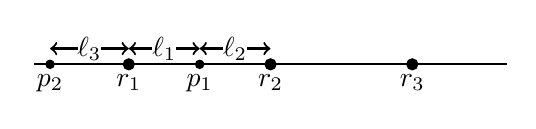
\begin{tikzpicture}
    
        
        \draw[black,thick] (0, 0) -- (6, 0);
        
        \filldraw[black] (0.2, 0) circle (1.5pt)
        node[anchor=north]{$p_2$};
        
        \draw[thick, <-] (0.2, 0.2) -- (0.55, 0.2); 
        \node[] at (0.7,0.2) {$\ell_3$};
        \draw[thick, ->] (0.85, 0.2) -- (1.2, 0.2);
        
        \filldraw[black] (1.2, 0) circle (2pt) node[anchor=north]{$r_1$};
        
        \draw[thick, <-] (1.2, 0.2) -- (1.5, 0.2);
        \node[] at (1.65,0.2) {$\ell_1$};
        \draw[thick, ->] (1.8, 0.2) -- (2.1, 0.2);
        
        \filldraw[black] (2.1, 0) circle (1.5pt)
        node[anchor=north]{$p_1$};
        
        \draw[thick, <-] (2.1, 0.2) -- (2.4, 0.2);
        \node[] at (2.55,0.2) {$\ell_2$};
        \draw[thick, ->] (2.7, 0.2) -- (3, 0.2);
        
        \filldraw[black] (3, 0) circle (2pt) node[anchor=north]{$r_2$};
        
        \filldraw[black] (4.8, 0) circle (2pt) node[anchor=north]{$r_3$};
        
        
    \end{tikzpicture}
    \caption{Illustration of the robot sensing model. The segment is being covered by three robot guards $r_1 \sim r_3$. The coverage probability of $p_1$, falling between robots $r_1$ and $r_2$, is given as $\rho(\ell_1)+\rho(\ell_2)-\rho(\ell_1)\cdot\rho(\ell_2)$, and the coverage probability of $p_2$, covered only by $r_1$ is given as $\rho(\ell_3)$.}
    \label{fig:sc-sensing}
\end{figure}


For covering a line segment with a length of $\ell$ and sensing function of $\rho$, 
we denote as $\zeta: \mathbb{R}^+ \rightarrow \mathbb{N}^+$ a primitive for computing 
the minimum number of robots needed to achieve the required minimum covering 
probability of $\rho_0$. 
%Denote the primitive as $\zeta: \mathbb{R}^+ \rightarrow \mathbb{N}^+$.

Take the exponential decaying sensing probability function as an example, 
where $\rho(r) = e^{-c\cdot r}$, $c>0$ is some constant.
In this case, the maximum distance at the two ends to guarantee the sensing probability of $\rho_0$ is $d_1=-\ln (\rho_0)/c$. 
If a point is between two robots with distance $\ell_1$ and $\ell_2$ to the two robots, its sensing probability is bounded by

\begin{align*}
\rho(\ell_1) + \rho(\ell_2) - \rho(\ell_1)\cdot \rho(\ell_2)\geq 2e^{-\frac{c\cdot d}{2}} - e^{-c\cdot d}    \\
where\ d = \ell_1+\ell_2
\end{align*}

So, the required maximum distance between two neighboring robots is $d_2=-2\ln(1-\sqrt{1-\rho_0})/c$.
Therefore, the minimum number of robots required to cover a line segment with length $\ell$ is 
$\zeta(\ell) = \max(1, 1 + \lceil(\ell-2\cdot d_1)/d_2 \rceil )$.


\subsection{Problem Formulation}
In this paper, we work with a 2D compact (i.e., closed and bounded) workspace 
${\mathcal W} \subset \mathbb{R}^2$, which can contain a set of obstacles. 
An existing \emph{sweep schedule} is an input to the problem, which we
define the \emph{continuous monotone sweep schedule} for $\mathcal W$ as 
\begin{definition}[Continuous Monotone Sweep Schedule]
A function $P(t)$ that maps a positive timestamp $t$ to a continuous curve is a continuous monotone sweep schedule for $\mathcal W$ if $P(t)$ changes continuously, 
and for each point $p\in \mathcal W$, there exists a single $t'$ such that $p\in P(t')$.
\end{definition}

Intuitively, a continuous monotone sweep schedule defines a function 
that maps the time step to a 1-D curve in the workspace that sweeps 
through each point in $\mathcal W$ only once. 
%
Depending on the continuous curve, $P(t)$ could take various forms. For example, the sweep line may be straight in a search-and-rescue scenario. Or the sweep line may be circular in a search-and-capture scenario. 
%e a  
%vertical sweeping, circular shrinking, and so on. 
In the rest of this paper, we simply refer to a continuous monotone sweep schedule as a \emph{sweep schedule}. Next, we introduce the notions of \emph{arrival time} and \emph{monotone chain}.
%
\begin{definition}[Arrival Time]
For a search schedule $P(t)$, and a point in the workspace $o\in\mathcal W$,
the arrival time at $o$, $arrival(o)$, is defined as the time step $t$ when $o\in P(t)$.
\end{definition}

\begin{definition}[Monotone Chain]
For a bounded 2D chain: $\tau(s): [0,1]\rightarrow\mathcal{W}$, where $\tau$ is a continuous function, it is considered as a monotone chain to the search schedule $P(t)$ if and only if
\[s_1 < s_2 \Leftrightarrow arrival(\tau(s_1)) < arrival(\tau(s_2)).\]
\end{definition}
In a search schedule or plan, $P(t)$ may be intersected by obstacles. In this case, $P(t)$ is separated into multiple continuous segments; each of these segments requires a dedicated group of robots. That is, robots on one continuous segment cannot provide coverage of other segments. 

%\r{We may want to define the classes of $\mathcal W$ that we work with. We want to work on a class of environment than can be swept with scan lines. This means that the non-convex obstacles must be able to ``see'' the outside in a some sense.}

With the probabilistic robot sensing model, we formulate the robot team scheduling problem for a given sweep schedule as the following,
\begin{problem}
Given a sweep schedule $P(t)$ for a 2D region $\mathcal W$, and a group of robots with coverage capability function $\rho$, what is the minimum number of robots required to execute the sweep schedule on the sweep line, such that 
for every point $o$ in $\mathcal W$, the probability that $o$ is covered is at 
least some fixed $0 < \rho_0 \le 1$?
\end{problem}



\section{Optimal Robot Allocation}

% \newcommand{\bdag}{{\textsc DAG}}

Our proposed algorithm can be divided into two steps at the high level. 
In the first step, the algorithm conducts a \emph{generalized boustrophedon 
decomposition} for the given environment along the sweep line, 
which generates a \textit{directed acyclic graph} (DAG) representation 
of the workspace $\mathcal W$ for a given sweep schedule. 
Using the DAG, a max-flow-based algorithm is then applied to compute the 
minimum number of robots required for executing the sweep schedule, 
as well as the corresponding arrangement of robots.

\subsection{Generalized Boustrophedon Decomposition}
In solving search and coverage problems, various decomposition techniques 
have been proposed, including trapezoidal, Voronoi, boustrophedon, Morse decompositions, 
and so on \cite{huang2001optimal, choset2000coverage, breitenmoser2010voronoi, acar2002morse}.
For our robot allocation task, it is also natural to start with a decomposition 
of the environment. 
However, we need a decomposition supporting non-straight 
boundaries between the decomposed cells, created by the sweep schedule. 
For this, we propose a generalization of boustrophedon decomposition. 

Before describing the generalization of boustrophedon decomposition, 
we briefly introduce boustrophedon decomposition (readers are referred to 
\cite{choset2000coverage} for further details), which in turn is based on 
trapezoidal decomposition. The difference is that it removes the sweeping 
events that cross inner vertices. As illustrated in Fig.~\ref{fig:trebou},
compared with trapezoidal decomposition, boustrophedon decomposition 
has fewer cells, which leads to fewer (back-and-forth) boustrophedon motions.

\begin{figure}[ht]
    \centering
    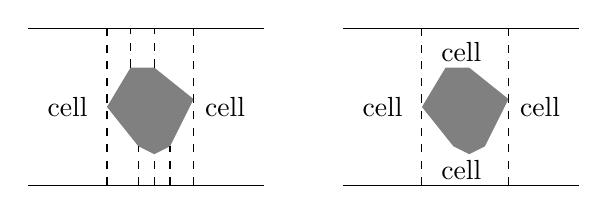
\begin{tikzpicture}
    % \fill[black] (0, 0) -- (1.9, 0.1) -- (1.3, 1) -- (1.85, 1.6) -- (0.1, 1.6) -- (0.7, 0.9) -- cycle;
    \fill[gray] (0, 0) -- (0.4, -0.5) -- (0.6, -0.6) -- (0.8, -0.5) -- (1.1, 0.1) -- (0.6, 0.5) -- (0.3, 0.5) -- cycle;
    \draw (-1, - 1) -- (2, -1); 
    \draw (-1, 1) -- (2, 1); 
    \draw[dashed] (0, -1) -- (0,1);
    \draw[dashed] (0.4, -1) -- (0.4,-0.5);
    \draw[dashed] (0.6, -1) -- (0.6,-.6);
    \draw[dashed] (0.8, -1) -- (0.8,-0.5);
    \draw[dashed] (1.1, -1) -- (1.1,1);
    \draw[dashed] (0.6, 0.5) -- (0.6,1);
    \draw[dashed] (0.3, 0.5) -- (0.3,1);
    
    \node[text=black] at (-0.5, 0.0) {cell};
    \node[text=black] at (1.5, 0.0) {cell};
    
    \fill[gray] (4, 0) -- (4.4, -0.5) -- (4.6, -0.6) -- (4.8, -0.5) -- (5.1, 0.1) -- (4.6, 0.5) -- (4.3, 0.5) -- cycle;
    
    \draw (3, - 1) -- (6, -1); 
    \draw (3, 1) -- (6, 1); 
    
    \draw[dashed] (4, -1) -- (4, 1);
    \draw[dashed] (5.1, -1) -- (5.1, 1);
    
    
    \node[text=black] at (3.5, 0.0) {cell};
    \node[text=black] at (4.5, -.8) {cell};
    \node[text=black] at (4.5, 0.7) {cell};
    \node[text=black] at (5.5, 0.0) {cell};

    \end{tikzpicture}
    \caption{[left] A trapezoidal decomposition, creating a total of $9$ cells. [right]
    Boustrophedon decomposition of the same environment, creating only $4$ cells.}
    \label{fig:trebou}
\end{figure}

We extend the boustrophedon decomposition from using only vertical sweep lines 
to allow the use of any \emph{continuous monotone sweep schedule}.
We are given a sweep schedule $P(t)$ for a workspace $\mathcal W$, 
which could take any curved form (see Fig.~\ref{fig:Bou}).
By following the sweep schedule, it is possible to
construct a decomposition of $\mathcal W$, based on the events of cell
splitting and merging. 

\begin{figure}[ht]
    \centering
    % \includegraphics[width = .3\textwidth]{fig/bou.eps}
    \begin{overpic}[width = .4\textwidth]{chapters/sc/fig/genbou.eps}
    \put(8, 35){$v_1$}
    \put(20, 10){$v_2$}
    \put(20, 30){$v_3$}
    \put(36.5, 42){$v_4$}
    \put(55, 20){$v_5$}
    \put(50, 40){$v_6$}
    \put(80, 30){$v_7$}
    \end{overpic}
    \caption{Suppose we have a sweep schedule that sweeps the environment from left 
    to right, with curved sweep fronts. 
    The curves, as they cross critical vertices of objects, are shown as the 
    dashed lines.
    The generalized boustrophedon decomposition decomposes and $\mathcal W$ into 
    $7$ cells, $v_1\sim v_7$. 
    %
    It is important to note here that, for any continuous monotone sweep schedule,
    a decomposition can be obtained. 
    }
    \label{fig:Bou}
\end{figure}


\begin{theorem}
A sweep schedule can be organized in a DAG by the generalized boustrophedon decomposition.
\end{theorem}

\begin{proof}
Following the sweep schedule, we can conduct a generalized boustrophedon 
decomposition of the workspace $\mathcal W$. 
%
A node in the DAG will represent a cell after the decomposition, whose 
parents and children are the predecessor and successor cells along the 
sweep schedule. 

Additionally, we add a source node that links to all nodes without a parent 
and add a terminal node that links from all nodes without a child.
%
Since obstacles in the environment can contain concave vertices, we must 
consider two special cases involving concave vertices for the construction of DAG, 
as illustrated in Fig.~\ref{fig:concave_vertices}. 
%
When a line segment of the sweep schedule ends at a concave vertex, 
the corresponding node in the DAG is linked to the terminal node $t$.
When a line segment of the sweep schedule starts at a concave vertex,
the corresponding node in the DAG is linked from the source node $s$.
In mapping these scenarios to detailed plans, it means that 
some robots will start later or end earlier compared with 
others.
% \end{remark}

\begin{figure} [ht]
    \centering
    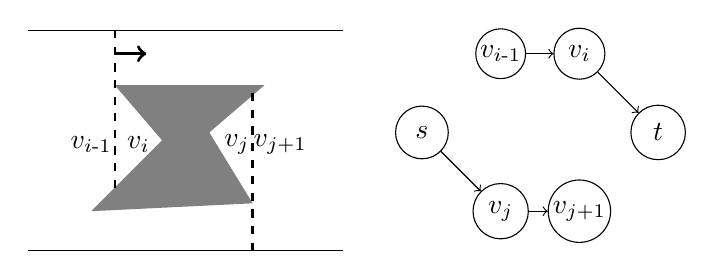
\begin{tikzpicture}
    \fill[gray] (-0.2, 0) -- (1.85, 0.1) -- (1.3, 1) -- (2.0, 1.6) -- (0.1, 1.6) -- (0.7, 0.9) -- cycle;
    \draw (-1, - 0.5) -- (3, -.5); 
    \draw (-1, 2.3) -- (3, 2.3); 

    \draw[dashed, line width=0.9pt, black] (0.1, 2.3) -- (0.1, 0.3);
    \draw[dashed, line width=0.9pt, black] (1.85, 1.5) -- (1.85, -0.5);
    
    
    \draw(-0.2, 0.85) node[text=black] { $v_{i\text{-}1}$};
    \draw(0.4, 0.85) node[text=black] {$v_i$};
    \node[text=black] at (1.65, 0.85) {$v_j$};
    \node[text=black] at (2.2, 0.85) {$v_{j\text{+}1}$};
    
    \draw(4, 1.0) node [circle, radius = 0.12, draw, inner sep=4.5](s){ $s$};
    
    \draw(5, 2.0) node [circle, radius = 0.12, draw, inner sep=0.8](vi1){ $v_{i\text{-}1}$};
    \draw(6, 2.0) node [circle, radius = 0.12, draw, inner sep=3](vi){ $v_{i}$};
    
    \draw(5, 0.0) node [circle, radius = 0.12, draw, inner sep=3](vj){ $v_{j}$};
    \draw(6, 0.0) node [circle, radius = 0.12, draw, inner sep=0.8](vj1){ $v_{j\text{+}1}$};
    
    \draw(7, 1.0) node [circle, radius = 0.12, draw, inner sep=4.5](t){ $t$};
    
    \draw[->] (vi) -- (t);
    \draw[->] (vi1) -- (vi);
    
    \draw[->] (vj) -- (vj1);
    \draw[->] (s) -- (vj);
    
    \draw[very thick, ->] (0.1, 2.0) -- (0.5,2.0);
    \end{tikzpicture}
    \caption{An example that contains two concave scenarios. As a result of the DAG construction, some robots will
    start their work at $v_j$ (by having $s$ as its parent) and some robots will end their work at $v_i$ (by having $t$ as its child).}
    \label{fig:concave_vertices}
\end{figure}
\end{proof}

% \begin{remark}



The implementation of the generalized boustrophedon decomposition is similar 
to vertical decomposition, we provide here an implementation 
Alg.~\ref{alg:genbou} adapted from \cite{lavalle2006planning} under the 
\emph{generation position} assumption (i.e., there are no degenerative 
settings).
%
Basically, the algorithm works by maintaining a binary search tree for 
\emph{boundary chains} representing cell boundaries. The algorithm considers 
two types of events during the sweeping process: splitting a cell into two 
cells and merging two cells into one cell.
%
Since the time cost mainly comes from maintaining the binary search tree of 
chains, with an efficient implementation, Alg.~\ref{alg:genbou} requires 
$O(n \log n)$ time, where $n$ is the complexity of the environment. 


\subsection{Reduction to Circulation with Demand}
Since we are working with \emph{monotone sweep schedules}, for any point $p$ in 
$\mathcal W$, it can only be contained in $P(t')$ for a single $t'$, i.e., each 
point $p \in \mathcal W$ is only swept once. 
%
Denote the length of the line segment where it is contained as $L$, which 
requires at least $\zeta(L)$ robots inside that segment at time $t'$
(recall that $\zeta$ is the primitive defined in Sec.~\ref{sec:sensing}).
%
For each decomposed cell, the minimum number of robots required is $\zeta(l_{max})$, where $\ell_{max}$ 
is the maximum length of the sweep line inside that cell.
%
Given a DAG $G(V,E)$ that represents the sweep schedule, the arrangement problem of the robots along the sweep line can be transformed into a network 
flow problem on the DAG.
%
For each node $v\in G$, there is a requirement of coverage for the node, 
$demand(v)$, which can be computed as $\zeta(v.\ell_{max})$.
%
Given the DAG and the demands, we are then to ``flow'' the robots through 
the schedule, allocating a certain number of robots to each decomposed cell 
along the way to satisfy these demands. 
%

Specifically, our problem may be further cast as a \emph{circulation with demand} 
problem \cite{kleinberg2006algorithm}, with the following augmentation. We replace 
each node $v$ in $G$ with two vertices $v_1$ and $v_2$ and replace every edge 
$uv$ in the previous graph with edge $u_2 v_1$, as illustrated in Fig.~\ref{fig:flow}. 
The edge between $v_1$ and $v_2$ has flow demand of $demand(v)$. 
The following minimum circulation with demand problem is then obtained.

\begin{algorithm}[h!]
\SetKwFunction{genbou}{GenBouDecomp}
%\begin{small}
\KwData{$P(t)$: a sweep schedule. $\mathcal W$: the workspace.}
\KwResult{a DAG from the decomposition.}
\vspace{1mm}
\SetKwComment{comment}{\%}{}
\DontPrintSemicolon
\SetKw{arrival}{Arrival}

1. Separate the boundaries of obstacles into a set of \emph{monotone chains},
where each chain has the points on it \emph{arrival time} arranged in an 
increasing order.;\;
\vspace{0.5mm}
% Denote $k$ as the number of chains obtains;\;

2. $T\gets$ A binary search  tree of the chains\;
\vspace{0.5mm}

3. Construct an \emph{event array} that contains the events of the start of a chain and the end of a chain, sorted by their occurrence time during the sweep.\;
\vspace{0.5mm}

4. Iterate over the event array, which inserts and deletes chains from the binary search tree $T$, while making sure that $T$ represents the current order of the chains.\;
\vspace{0.5mm}
%\comment{\begin{footnotesize}With the general position assumption, the events comes as a paired operation for either deletion or insertion of chains \end{footnotesize}}

% When two chains are added to $T$, a cell is split into two new cells in the case of convex
% vertex or a new cell is created.  An edge from $s$ is added for a concave vertex.\;
When two chains are added to $T$, a cell is split into two new cells in the case of a convex vertex, or a new cell is created for a concave vertex, where an edge directed from $s$ is added.\;
% When two chains are removed from $T$, two cells are merged into a new cell in the case of 
% convex vertex or a cell disappears. An edge is added to $t$ for a concave vertex.\;
When two chains are removed from $T$, two cells are merged into a new cell in the case of a convex vertex or a cell disappears for a concave vertex, where an edge is added directed to $t$.\;

5. Return the DAG constructed based on $P(t)$.
%\end{small}
\caption{\protect\genbou{$P$, $\mathcal{W}$}: Generalized Boustrophedon Decomposition} 
\label{alg:genbou}
\end{algorithm}

\begin{figure}[h]
    \centering
    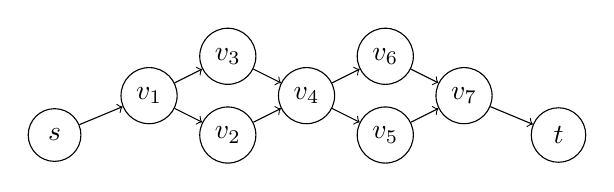
\begin{tikzpicture}
    % \node[circle](v1){$v1$};
    % \node[circle](v2){$v2$};
    % \draw[->] (v1.east) -- (v2.west);
    \draw(0,0) node [circle, radius = 0.12, draw](v1){ $v_1$};
    \draw(1, -0.5) node [circle, radius = 0.12, draw](v2){ $v_2$};
    \draw(1, 0.5) node [circle, radius = 0.12, draw](v3){ $v_3$};
    \draw(2, 0.0) node [circle, radius = 0.12, draw](v4){ $v_4$};
    \draw(3, -0.5) node [circle, radius = 0.12, draw](v5){ $v_5$};
    \draw(3, 0.5) node [circle, radius = 0.12, draw](v6){ $v_6$};
    \draw(4, 0.0) node [circle, radius = 0.12, draw](v7){ $v_7$};
    
    \draw(-1.2, -.5) node [circle, radius = 0.2, draw,inner sep=4.5](s){ $s$};
    
    \draw(5.2, -.5) node [circle, radius = 0.2, draw,inner sep=4.5](t){ $t$};
    
    \draw[->] (v1) -- (v2);
    \draw[->] (v1) -- (v3);
    \draw[->] (v2) -- (v4);
    \draw[->] (v3) -- (v4);
    \draw[->] (v4) -- (v5);
    \draw[->] (v4) -- (v6);
    \draw[->] (v5) -- (v7);
    \draw[->] (v6) -- (v7);
    
    \draw[->] (s) -- (v1);
    \draw[->] (v7) -- (t);
    \end{tikzpicture}
    \caption{The constructed DAG from the example in Fig.~\ref{fig:Bou}}
    \label{fig:sc-DAG}
\end{figure}


\begin{algorithm}[h!]
%\begin{small}
\DontPrintSemicolon
\SetKwFunction{mindag}{MinSweepDAG}
\SetKwFunction{dflow}{MinCirculationWithDemand}
\SetKwFunction{addedge}{add\_edge}
\SetKwFunction{addvertex}{add\_vertex}
\KwData{$dag(V, E)$: the DAG obtained from \genbou. $\zeta$: the sensing requirement primitive function.}
\KwResult{$dag$: the updated $dag$ with the robot allocation information}
\vspace{0.5mm}
$G'\gets$ a new empty graph;\;
\vspace{0.5mm}

\For{$v\in dag$}{
\vspace{0.5mm}
    $G'$.\addvertex$(v_1),$ $ G'$.\addvertex($v_2$);\;
\vspace{0.5mm}
    
    $G'.$\addedge($v_1, v2$, capa=$\infty$, demand=$\zeta(v.\ell_{max})$);\;
\vspace{0.5mm}
    
    \For{$u\in dag.neighbor[v]$}{
\vspace{0.5mm}
        $G'$.\addedge($v_2$, $u$, capa=$\infty$, demand=0);\;
    }
}
\vspace{0.5mm}

\dflow($G'$);\;
\vspace{0.5mm}

\For{$v\in dag$}{
\vspace{0.5mm}
    $dag.v.guards\_num\gets$ $G'.flow[v_1][v_2]$;\;
    
\vspace{0.5mm}
    \For{$u\in dag.neighbor[v]$}{
        $dag.flow[v][u] = G'.flow[v_2][u_1]$;\;
    }
    
}


\Return{$dag$}\;

% \begin{small}

%\end{small}
\caption{\protect\mindag{$dag$, $\zeta$}{}}
\label{alg:mindag}
\end{algorithm}

\begin{figure*}[h!]
\vspace{2mm}
    \centering
    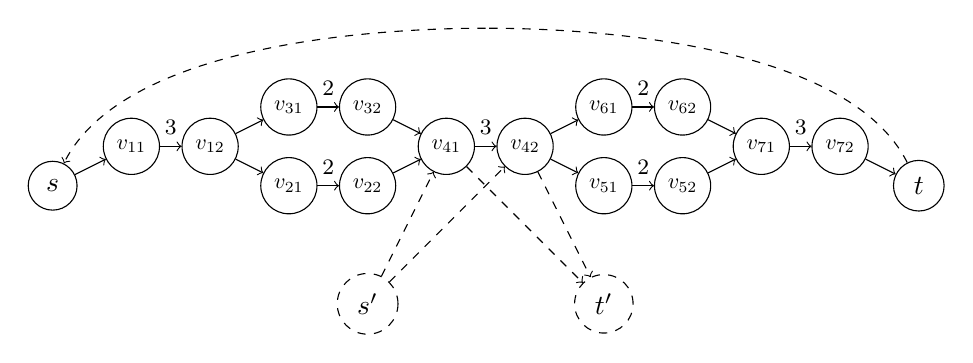
\begin{tikzpicture}[scale = 1, every node/.style={inner sep=4}]
    \draw(0,0) node [circle, draw, scale = 0.8](v11){ $v_{11}$};
    \draw(1,0) node [circle, draw, scale = 0.8](v12){ $v_{12}$};
    
    \draw(2, -0.5) node [circle, draw, scale = 0.8](v21){ $v_{21}$};
    \draw(3, -0.5) node [circle, draw, scale = 0.8](v22){ $v_{22}$};
    
    \draw(2, 0.5) node [circle, draw, scale = 0.8](v31){ $v_{31}$};
    \draw(3, 0.5) node [circle, draw, scale = 0.8](v32){ $v_{32}$};
    
    \draw(4, 0.0) node [circle, draw, scale = 0.8](v41){ $v_{41}$};
    \draw(5, 0.0) node [circle, draw, scale = 0.8](v42){ $v_{42}$};
    
    \draw(6, -0.5) node [circle, draw, scale = 0.8](v51){ $v_{51}$};
    \draw(7, -0.5) node [circle, draw, scale = 0.8](v52){ $v_{52}$};
    
    \draw(6, 0.5) node [circle, draw, scale = 0.8](v61){ $v_{61}$};
    \draw(7, 0.5) node [circle, draw, scale = 0.8](v62){ $v_{62}$};
    
    \draw(8, 0.0) node [circle, draw, scale = 0.8](v71){ $v_{71}$};
    \draw(9, 0.0) node [circle, draw, scale = 0.8](v72){ $v_{72}$};
    
    \draw(-1, -.5) node [circle, draw](s){ $s$};
    \draw(10, -.5) node [circle, draw](t){ $t$};
    
    \draw[->] (v12) -- (v21);
    \draw[->] (v12) -- (v31);
    \draw[->] (v22) -- (v41);
    \draw[->] (v32) -- (v41);
    \draw[->] (v42) -- (v51);
    \draw[->] (v42) -- (v61);
    \draw[->] (v52) -- (v71);
    \draw[->] (v62) -- (v71);
    
    \draw[->] (v11) -- node[above]{\footnotesize $3$} (v12) ;
    \draw[->] (v21) -- node[above]{\footnotesize $2$} (v22) ;
    \draw[->] (v31) -- node[above]{\footnotesize $2$} (v32) ;
    \draw[->] (v41) -- node[above]{\footnotesize $3$} (v42) ;
    \draw[->] (v51) -- node[above]{\footnotesize $2$} (v52) ;
    \draw[->] (v61) -- node[above]{\footnotesize $2$} (v62) ;
    \draw[->] (v71) -- node[above]{\footnotesize $3$} (v72) ;
    
    \draw[->] (s) -- (v11) ;
    \draw[->] (v72) -- (t) ;
    
    \draw[dashed] (t) .. controls(9, 1.5) and (5, 1.5) .. (4.5, 1.5);
    \draw[dashed,->] (4.5,1.5) .. controls(4,1.5) and (0,1.5) .. (s);
    
    \draw(3, -2) node [circle, draw, dashed] (s'){$s'$};
    \draw(6, -2) node [circle, draw, dashed] (t'){$t'$};
    
    \draw[dashed,->] (s') -- (v41);
    \draw[dashed,->] (v41) -- (t');
    
    \draw[dashed,->] (s') -- (v42);
    \draw[dashed,->] (v42) --  (t');
    
    \end{tikzpicture}
    \caption{Transform the DAG in Fig.~\ref{fig:DAG} into a circulation with demand problem. 
    The value above each edge represents the demand of the edge, which is eliminated when it is zero.
    The source node is $s$, and the target node is $t$. $s'$ and $t'$ are the auxiliary source and target for solving the ``circulation with demand'' problem.
    Also, auxiliary edges are added between $s', t'$ and every other vertex.}
    \label{fig:sc-flow}
\end{figure*}


\begin{problem}[Minimum Circulation with Demand]
There is a graph $G(V,E)$, where $s,t$ are the source and terminal nodes. 
Every edge $uv$ in $G$ has a demand of $d(uv)$ and a capacity of $c(uv)$. 
Compute minimal network flow from $s$ to $t$ that saturates all the edge 
demands.
\end{problem}

Readers are referred to \cite{kleinberg2006algorithm} for %detailed algorithm   description and proof of correctness 
the details of the classical ``circulation with demand'' problem solution with max-flow. 

Alg.~\ref{alg:mindag} outlines the operations
used in this section. We note that the 
graph data structure needs to have the functionality of adding vertex and adding 
edge with edge demand, and $G'.flow[v_1][v_2]$ denotes the flow from $v_1$ to $v_2$ on $G'$.
% By solving the maxflow problem, we 

\subsection{The Complete Allocation Algorithm}
The overall algorithm for robot allocation is described as in Alg.~\ref{alg:overall}.
To analyze the running time of Alg.~\ref{alg:overall} for a polygonal environment, 
we denote the environment complexity (number of vertices) as $n$. 
As mentioned in the previous section, the generalized boustrophedon decomposition takes $O(n\log n)$ time. 
As the generation of a node in the DAG comes from some chain insertion or deletion events, and an event would require one vertex to happen, 
there is at most $O(n)$ decomposed cells, i.e., nodes in the DAG. 
Similarly, adding edges between nodes comes from some chain insertion or deletion events, and the number of events is at most $O(n)$. 
So, both the number of edges and the number of nodes in the DAG is $O(n)$.
Moreover, it is easy to see that the DAG is a planar graph since a node corresponds to a decomposed cell, and there is an edge between nodes only if the two corresponding cells are adjacent.
The circulation with demand problem requires solving two max-flow problems based on the DAG. 
If we use the push-relabel algorithm \cite{cheriyan1989analysis} that runs in $O(V^2\sqrt{E})$, solving the max flow for this problem will cost $O(n^{2.5})$, 
% If we use the Dinic's algorithm \cite{dinitz1970algorithm} that runs in $O(V^2E)$, solving the max flow for this problem will cost $O(n^{3})$, 
since $|V|, |E| = O(n)$.% for planar graphs. 

\begin{algorithm}[ht]
%\begin{small}
\SetKwFunction{minsweep}{MinSweep}
\KwData{$P(t)$: a sweep schedule. $\mathcal W$: a compact workspace.
$\rho_0$: required sensing probability guarantee.
% Primitive function $\zeta$ to compute the minimum number of line guards required for a continuous line segment.
}
\KwResult{$n$: the minimum number of robot guards required. $plan$: the corresponding allocation plan}%, embedded in a DAG.}
\SetKwComment{comment}{\%}{}

\vspace{1mm}
Construct $\zeta$ based the sensing model and $\rho_0$\;
\vspace{1mm}

\begin{small}
\comment{Primitive function $\zeta$ is to compute the minimum number of robots required for a continuous line segment}
\end{small}
\vspace{1mm}
$dag\leftarrow \genbou(P, {\mathcal W})$;\;

\vspace{1mm}
$dag\gets \mindag(dag, \zeta)$;\;

\vspace{1mm}
$plan\gets dag$;\;

\vspace{1mm}
\begin{small}
\comment{The plan of the robots can be constructed based on the flow on the $dag$.} 
\end{small}

\vspace{1mm}
\Return{$dag.s.guards\_num$, plan};\;
% Step 2. Construct corresponding DAG for the robot sweep schedule, as well as 
% the minimum number of robots required: $\zeta(\ell_m)$ for each cell\;

% Step 3. Run the minimum flow with demand algorithm on the transformed DAG, which results in the allocation of the robots\;
%\end{small}
\caption{\protect\minsweep{$P, {\mathcal{W}}, \rho_0$}: Computing Minimum Number of Robots for a Sweep Schedule}
\label{alg:overall}
\end{algorithm}



\begin{remark}
In the case of having a fixed number of robots, 
and the objective is to 
maximize the minimum coverage probability of a point in $\mathcal W$.
We can apply binary search on the minimum coverage probability we can guarantee, where Alg.~\ref{alg:overall} can be used to decide whether some coverage probability can be guaranteed by the fixed number of robots.
% The algorithm is detailed out in Alg.~\ref{alg:fixednum}
%\r{I think a remark is enough to say it}
\end{remark}

% \begin{algorithm}[ht]
% \begin{small}
% \SetKwFunction{maxprob}{MaxProb}
% \KwData{ $P(t)$: a sweep schedule. 
% $\mathcal W:$ a compact workspace.  $k$: the number of robots. }
% \KwResult{an allocation plan for $k$ robots to achieve 
% maximum guaranteed coverage probability, embedded in a DAG.}

% $\rho_{min}, \rho_{max}\leftarrow  0$, $1$;\;

% \While{$\rho_{max}-\rho_{min} \geq \varepsilon$}{
%     % \State Construct $\zeta$ based on $\rho_{mid}=(\rho_{min} + \rho_{max})/{2}$\\
%      $n$, $plan$ $\gets \minsweep(P, {\mathcal W}, \rho_{min})$;\;
    
%     \eIf{$n > k$}{
%          $\rho_{max} \gets \rho_{mid}$;\;
%     }{
%          $\rho_{min} \gets \rho_{mid}$;\;
%     }

% }
% \Return{$\rho_{min}$, plan}
% \end{small}
% \caption{\maxprob$(P, \mathcal{W}, k)$: Maximizing the Sensing Probability Guarantee for a Sweep Schedule with Fixed Number of Robots }
% \label{alg:fixednum}
% \end{algorithm}


\subsection{Simulation Evaluation}
In this section, we perform a numerical evaluation of our proposed method
with two goals: (1) confirms the scalability and (2) observe the behavior 
of the method as input parameters change. 
%
We implemented our proposed algorithms in C++. Dinic's algorithm is used to solve the max-flow problem \cite{dinitz1970algorithm} for simplicity. 
The methods are evaluated at an Intel\textsuperscript{\textregistered} Core\textsuperscript{TM} i5-10600K CPU at 4.1HZ.
%
For the three use cases (~\ref{fig:sc-sweep} (b)(c)(d)), we
programmatically create a large number of test cases, with up to 
$6,000$ randomly generated polygonal obstacles. 
%
The number of vertices of each polygon ranges from 3 to 50, making the total vertices up to 
$100,000+$. 
%
~\ref{fig:sc-cases} shows the largest problem instances for the experiments with 
around $100,000$ vertices.
\begin{figure}[ht]
    \centering
    \includegraphics[width=.95\linewidth]{chapters/sc/fig/cases.png}
    \caption{Examples of programmatically generated test environments with total 
    vertices around $100,000$.}
    \label{fig:sc-cases}
\end{figure}

\textbf{Algorithm performance.} In a first set of evaluations, under an exponentially 
decaying sensing 
model, $\rho(r) = e^{-c\cdot r}$, we test the performance of our algorithm over 
the set of instances. Example allocation of robots along the sweep frontiers for 
the three cases are shown in ~\ref{fig:sc-sweep}(a) and ~\ref{fig:sc-simulations}. 
We limited the number of robots to be small so that the trajectories are more easily 
observed. It can be seen that the trajectories can vary significantly along the 
sweep frontiers for each case. 
% The first setting uses vertical sweep as the search schedule to sweep a rectangle.
% The second setting uses circular sweep, where guards are tasked to
% sweep $\mathcal{W}$ in a circular expansion manner.
% The thirst setting uses radial expansion as the search schedule, that is 
% a group of guards are tasked to sweep a circular regions in a radial rotational manner.
\begin{figure}[ht]
    \centering
    % \includegraphics[width=.45\linewidth]{fig/vertical_large-eps-converted-to.pdf}
    \includegraphics[width=.45\linewidth]{chapters/sc/fig/circular_sol-eps-converted-to.pdf}\hspace{2mm}
    \includegraphics[width=.45\linewidth]{chapters/sc/fig/rotational_sol-eps-converted-to.pdf}
    
    \caption[Example robot trajectories]{Example robot trajectories computed by our method for circular and radial 
    sweep use cases, respectively.
    }
    \label{fig:sc-simulations}
\end{figure}

In ~\ref{fig:sc-simulations_runtime}, the computational performance is thoroughly 
evaluated. As can be observed, our method scales fairly well, taking less than two seconds
to handle all cases, even those involving over $100,000$ vertices. 
%
%We show the running time information in ~\ref{fig:simulations_runtime}. 
%The algorithm scale up reasonably to $10^5$ vertices in around $1.5s$ for the three sweep patterns. 
Interestingly, the experimental running time is almost linear, even using the less efficient Dinic's algorithm. 
%
We suspect the near linear running time is due to the fact that the DAG is 
a planar graph; studies show that max-flow for planar graphs can be computed 
in $O(n\log n)$ \cite{borradaile2009n}. 
%
Although the graph constructed when solving the ``circulation with demand'' problem is not planar, large portions are planar. 
This could reduce the actual time complexity of running the max-flow algorithm.

\begin{figure}[h]
\vspace{2mm}
    \centering
    \includegraphics[width=0.5\linewidth]{chapters/sc/fig/runtime-eps-converted-to.pdf}
    \caption{Running time in seconds with respect to environment complexity (number of vertices). }
    \label{fig:sc-simulations_runtime}
\end{figure}

\textbf{Different environment settings.}
Lastly, we evaluate the impact of environmental changes, considering factors including the spatial distribution of polygonal obstacles as well as 
the size distribution of the obstacles. 
%
All in all, three settings are considered: (1) The polygons are regularly distributed 
and are of similar size, (2) the polygons are randomly distributed and are of similar size,
and (3) the polygons are regularly distributed, and their sizes can vary dramatically. 
The first and the third settings are illustrated in the top row of ~\ref{fig:sc-runtime_env}.
%
For these settings, we compare the time it takes to compute solutions for many polygonal
obstacles and also the number of robots required to achieve $80\%$ probabilistic guarantee 
under the exponential decay sensing model.
%
As we can observe, there is little difference as the settings change. 

\begin{figure}[h]
    \centering
    \hspace{5mm}
    \includegraphics[width = 0.44\linewidth]{chapters/sc/fig/expr_inst_regular-eps-converted-to.pdf}\hspace{1mm}
    \includegraphics[width = 0.44\linewidth]{chapters/sc/fig/expr_inst_varscale-eps-converted-to.pdf}
    \vspace{3mm}
    
    \includegraphics[width=.47\linewidth]{chapters/sc/fig/runtime_env-eps-converted-to.pdf}
    \includegraphics[width=.48\linewidth]{chapters/sc/fig/n_env-eps-converted-to.pdf}
    \caption[Random instance and runtime time]{
    [top] Random instance with regularly distributed obstacles and instance with random obstacle scales and positions.
    [bottom] Running time for different randomly generated environments and the number of robots required for different randomly generated environments.}
    \label{fig:sc-runtime_env}
\end{figure}

%Based on the evaluation, one somewhat interesting conclusion we can draw is 
%that, the solution to the robot allocation task for carrying out pre-determined 
%sweep schedule is fairly ``stable''; it is unlikely to have dramatic 
\subsection{Conclusion }%\& Future work}

In this paper, we studied the problem of allocating a minimum number of robots for a sweep schedule with a probabilistic line sensing model, where a desired level of scanning quality can be guaranteed. 
Towards this, a novel decomposition technique is proposed that generalizes the well-known boustrophedon decomposition. The decomposition leads naturally to  a transformation of the problem into a network-flow problem. Due to the decomposition and the transformation, our proposed algorithm runs in low polynomial time and even near $\Tilde{O}(n)$ in simulation experiments for polygonal environments, where $n$ is the complexity of the environment, measured as the number of vertices of polygons. Extensive simulation-based evaluation corroborates the effectiveness of our algorithm, which is applicable to multiple types of environments.  

% In future work, we would like to take the current study in several directions. 
% One further step is to overcome the discontinuities in the robot paths generated. 
% As can be seen in the example trajectory of the robots, 
% when the sweep line crosses vertices, there exists position ``jumps'', though these jumps are transitions inside the sweep line and does not cross objects.
% Intuitively, this requires the sweep line to stop at that position until the robot moved to the next point, or the robot is much faster than the sweep line.
% A second direction is the adaptation to more versatile sweeping plan.
% This work limits the robot to stay on the given search frontier;
% it will be more natural to allow robots to shortly leave the search frontier, e.g., possibly going into or out of a concave region.




    
\chapter{Realworld Application}
\thispagestyle{myheadings}

This chapter discusses a relevant real-world application in the placement of UV (ultraviolet) lights 
to cover the surface of an environment for sanitization purposes. The problem can be seen as an extension
of the art-gallery problem \cite{o1987art}, and thus computationally intractable.
Still, a combined integer programming and classical local search approach can be used to
solve the problem effectively. The method is evaluated on three real scenarios: 
the interior of a bus, a subway or an ICU room. 

% text of this chapter goes here
\section{Covering 3D surfaces}

\def\spoc{{\texttt{{SPOC}}}\xspace}
\def\osg{{\texttt{{OSG}}}\xspace}

\subsection{Introduction}

We perform a systematic study of a class of mobile sensor\footnote{As will be explained, ``mobile sensor'' is used here in a broad sense.} deployment optimization problems targeting the coverage of 2D surfaces embedded in 3D domains, applicable to a broad set of practical settings, for example: (1) the selection of surveillance camera locations for maximizing the joint coverage of an art museum, (2) the deployment of mobile robots with range-based sensing apparatus for the monitoring of complex 3D terrains with quality assurances, and (3) the optimization of UVC light source locations for disinfecting interior surfaces of public indoor spaces, e.g., airplanes, buses, hospital rooms, and schools (~\ref{fig:ex}), which is of key relevance to the ongoing COVID-19 pandemic. Despite the problems' apparent differences, the above-mentioned tasks fall under the general problem of placing mobile sensors for optimizing some form of coverage. This work is devoted to providing such a unifying problem formulation, understanding its rich structural properties, and delivering effective computational methods for readily solving the multiple variations, which all have high application potentials.

\begin{figure}[!ht]
    \centering
    \includegraphics[width=0.95\columnwidth]{chapters/surf/fig/icu-expo.png}
    \vspace{1mm}
    %\hspace{-0.505\columnwidth}
    %\includegraphics[width=.48\columnwidth]{fig/icu_result_problem3_3.png}
    \caption{[left] The 3D model of an intensive care unit (ICU) in a hospital. [right] A near-optimal coverage of the ICU using three UVC light sources deployed on the ceiling of the room (shown as red discs) where a minimum level of exposure dose can be guaranteed. Each color (orange, green, pink) marks the covered surface locations of a given UVC source. Areas with insufficient exposure are also readily shown as scattered white regions, which can be eliminated through adding more UVC sources.}
    \label{fig:ex}
\end{figure}

As a summary of the research and its contributions, under a general formulation, three coverage optimization problems are examined that are based on \emph{visibility}, \emph{best quality}, and \emph{cumulative quality}, respectively. The visibility model only takes into account line-of-sight sensing. In the best quality model, the coverage quality of a point in the environment is determined by the closest visible sensor, i.e., the quality is determined by distance. A max-min optimization over this quantity is performed. In the cumulative quality model, the coverage of a point is the sum of coverage by all visible ``sensors''. For this model, the area over which a minimum quality can be guaranteed is maximized. Even in simpler 2D settings, these formulations, are known to induce significant computational challenges. They are frequently NP-hard and sometimes hard to approximate, which we briefly discuss. On the algorithmic side, we show how some of these problems can be approximately solved in polynomial time and then develop general integer programming methods, assisted with local improvements, for quickly computing high quality (i.e., $(1+\varepsilon)$-optimal) solutions. Extensive evaluations are performed over multiple realistic application scenarios, confirming the effectiveness of our algorithmic solutions. 

The general formulation and specific models investigated in this work have their origins in two main lines of research: Art Gallery \cite{o1987art,shermer1992recent,o2017visibility} and studies on mobile sensor networks, e.g., \cite{howard2002mobile,cortes2004coverage,martinez2007motion,krause2008near,schwager2009decentralized,hollinger2013sampling}. Our visibility-based model has deep roots in Art Gallery problems \cite{o1987art,shermer1992recent,o2017visibility}, which commonly assume a sensor model based on line-of-sight visibility\cite{lozano1979algorithm}; a main task is to guard every point in the interior of a bounded 2D regions (a point is guarded when it is visible to at least one of the guards). Depending on the exact formulation, guards may be placed on boundaries, corners, or the interior of the region. Not surprisingly, Art Gallery problems are typically NP-hard \cite{lee1986computational}. Other than Art Gallery, 2D coverage problems with other sensing models, e.g., disc-based, have also been considered \cite{thue1910dichteste,hales2005proof,drezner1995facility,cortes2004coverage,pavone2009equitable,pierson2017adapting}. Some formulations prevent the overlapping of individual sensing ranges \cite{thue1910dichteste,hales2005proof} while others seek to ensure a full coverage which often require overlapping sensor coverage.

In an influential body of work \cite{cortes2004coverage,martinez2007motion}, a gradient-based iterative method was devised that drives multiple mobile sensors to a locally optimal coverage configuration, with 
convergence guarantees. 
%
Whereas \cite{cortes2004coverage,martinez2007motion} assume availability of gradients {\em a priori}, such information can also be learned \cite{schwager2009decentralized}. 
%
Subsequently, the method is further extended to allow the coverage of non-convex and disjoint 2D domains \cite{schwager2009optimal} and to work for mobile robots with heterogeneous capabilities \cite{pierson2017adapting}. 
%
In contrast to these iterative local interaction-based methods, this work emphasizes the direct computation of globally optimal solutions under challenging 3D settings. 

 Distributed sensor coverage \cite{cortes2004coverage,schwager2009decentralized} builds on the study of facility location problems \cite{weber1929theory,drezner1995facility} examining the selection of facility (e.g., warehouses) locations that minimize the cost of delivery of goods to spatially distributed customers. These are known (e.g., in operations research and computer science) as clustering problems \cite{har2011geometric}, with many variations depending on the cost structure. Our investigation benefits from the vast literature on clustering and related problems, e.g., \cite{feder1988optimal,hochbaum1985best,gonzalez1985clustering,daskin2000new,shamos1975closest}.
%
Clustering problems are in turn related to packing \cite{hales2005proof}, tiling \cite{thue1910dichteste}, and Art Gallery problems \cite{o1987art,shermer1992recent}.

This work is a continuation of our systematic effort \cite{fenghangaoyu2019efficient,fengyu2020RAL,fengyu2020optimally} at tackling sensor coverage problems. Our earlier studies focus on 1D/2D sensors models covering 1D/2D domains, which are significantly less complicated than the 3D settings examined in the current study.

The rest of the paper is organized as follows. In Section~\ref{sec:preliminary}, we provide an umbrella problem statement and detail the three coverage models. Computational complexity of the formulations is briefly discussed. In Section~\ref{sec:algorithm}, we describe effective algorithmic solutions for solving these sensor coverage problems. Extensive evaluation results are provided in Section~\ref{sec:evaluation} containing multiple realistic application settings. We conclude the work in Section~\ref{sec:conclusion}.\label{sec:surf-intro}

\subsection{Preliminaries}\label{sec:surf-preliminary}
\subsection{Sensor Placement for Optimal Coverage: Formulations}
Let $\mathcal E \subset \mathbb R^3$ be a bounded three-dimensional workspace that is path-connected, e.g., a hilly terrain or an intensive care unit (ICU) in a hospital. We consider the problem of deploying $k$ ``mobile sensors'', $c_1, \ldots, c_k$, to guard a \emph{critical subset} $S$ embedded in the surface of $\mathcal E$, i.e., $S \subset \partial \mathcal E$ where $\partial$ is the boundary operator. For example, if $\mathcal E$ is a hospital ICU, $S$ may be a part of its interior surface. The sensors are to be deployed to achieve a globally optimal coverage of $S$ satisfying some prescribed objective, to be made more precise as the problems are further grounded for specific sensor models. We denote this broad class of problems as \emph{Sensor Placement for Optimal Coverage} (\spoc). 
%

The terms \emph{mobile sensor} and \emph{coverage} are used in a broad sense. Beyond traditional sensors that only collect information, we are interested in mobile robots with means to effect the environment as well. For example, a mobile robot may be equipped with a disinfecting light source (e.g., UVC) for eradicating harmful microbes (e.g., viruses and bacteria). Nevertheless, such settings can be nicely captured under a general sensor coverage formulation. 

In this study, we explore two common types of coverage models: \emph{visibility}-based and \emph{quality}-based. 
%
In a \emph{visibility}-based sensor coverage model, as the term suggests, a point $p \in S$ is considered covered by a sensor $c$ if $p$ is visible from $c$.
%, i.e., the straight line path between $p$ and $c$ does not intersect the 3D environment $\mathcal E$. 
When there are more than one sensor, a point $p$ is covered if it is visible from any sensor $c_i \in \{c_1, \ldots, c_k\}$. 
%
In a \emph{quality}-based model, the coverage quality of a point $p \in S$ is captured by some function that potentially depends on the sensors, the point $p$, and its neighborhood in $S$. For example, one type of quality measurement can be based on the inverse of the distance between a point $p$ and its closest sensor $c$. 

Formally, we capture the different sensor models under a unified function $f(c_1, \ldots, c_k, p, \mathcal E)$ whose co-domain is non-negative reals, i.e., $f: \mathbb R^{3k + 3} \times \mathcal E \to \mathbb R_+\cup\{0\}$. In what follows, $\mathcal E$ is omitted but understood to be part of the input to $f$. In this paper, the following instantiations are considered:
\begin{itemize}[leftmargin=4mm]
    \item Let $vis(p, c) = 1$ if the point $p$ is visible to the sensor $c$. Otherwise, $vis(p, c) = 0$. For example, an omni-directional visibility model would have $vis(p, c) = 1$ if the open line segment between $p$ and $c$ does not intersect $\mathcal E$. In a model based purely on \textbf{visibility},  
    \begin{align}
    f(c_1, \ldots, c_k, p) := \max_{1\le i \le k}vis(p, c_i).\label{f:1}
    \end{align}
    \item Let the \emph{coverage quality} of a point $p$ by a sensor $c_i$ be represented as a function $\phi(p, c_i) \in \mathbb R_+\cup\{0\}$. In a \textbf{quality maximization} sensor model,  the coverage quality for a point $p$ is determined by a single best sensor:  
    \begin{align}f(c_1, \ldots, c_k, p) := \max_{1\le i \le k} \phi(p, c_i)vis(p, c_i).\label{f:2}
    \end{align}
    \item In a \textbf{cumulative quality} sensor model, the overall quality of coverage at a point $p$ is the sum of the effects of all visible sensors:
    \begin{align}f(c_1, \ldots, c_k, p) := \sum_{1\le i \le k}\phi(p, c_i)vis(p, c_i).\label{f:3}
    \end{align}
\end{itemize}



All above models have direct and practical applications. 
A visibility model is applicable to the deployment of a network of $360^{\circ}$ cameras for monitoring. 
Letting $\phi(p, c_i) = \lVert pc_i\rVert^{-1}$ ($\lVert pc_i\rVert$ denotes the distance between $p$ and $c_i$), 
the quality maximization model becomes the $k$-center problem \cite{weber1929theory} if we optimize $\min_p f(c_1, \ldots, c_k, p)$, 
a broadly applicable problem. For the cumulative quality model, when the ``sensors'' are UVC lights, 
one may ask the question of how to optimally place these lights to ensure the highest percentage of $S$ can be exposed to sufficient UVC light for eradicating SARS-CoV-2 and other microbes. 
Here, a cumulative quality model clearly makes sense. 

To fully ground the discussion that follows, we formulate three concrete optimization problems, one for each of the above-mentioned sensor models. 

\begin{problem}[Visibility Maximization]\label{p:1} 
    Given $S \subset \partial \mathcal E$ with $\mathcal E \subset \mathbb R^{3}$, $c_i \in \mathbb R^3$, 
    $1 \le i \le k$, and $f(c_1, \ldots, c_k, p)$ from \eqref{f:1}, 
    determine a placement of $c_1, \ldots, c_k$ that maximizes the \ul{support of $f$}, i.e., 
    $supp(f) = \{p \in S \mid \max_{1\le i \le k}vis(p, c_i) >0\}.$  
\end{problem}

\begin{problem}[Quality Maximization]\label{p:2} 
    Given $S \subset \partial \mathcal E$ with $\mathcal E \subset \mathbb R^{3}$, $c_i \in \mathbb R^3$, 
    $1 \le i \le k$, and $f(c_1, \ldots, c_k, p)$ from \eqref{f:2} with $\phi(p, c_i) = \lVert pc_i\rVert^{-1}$, 
    determine a placement of $c_1, \ldots, c_k$ that maximizes the \ul{minimum coverage quality}, i.e., 
    $\min_{p \in S} \max_{1\le i \le k} \frac{vis(p, c_i)}{ \lVert pc_i\rVert}.$
\end{problem}

\begin{problem}[Cumulative Quality]\label{p:3} 
    Given $S \subset \partial \mathcal E$ with $\mathcal E \subset \mathbb R^{3}$, 
    $c_i \in \mathbb R^3$, $1 \le i \le k$, and $f(c_1, \ldots, c_k, p)$ from \eqref{f:3} with $\phi(p, c_i) = |lVert pc_i\rVert^{-2}\langle \hat{n}_p, \hat{n}_{pc_i} \rangle$ where $\hat{n}_p$ is the unit normal of $S$ at $p$ and $\hat{n}_{pc_i}$ is the unit vector in the direction from $p$ to $c_i$, 
    determine a placement of $c_1, \ldots, c_k$ that maximizes the \ul{coverage area where $f$ is above a given threshold} $\Phi > 0$,
    $supp(f - \Phi) = \{p \in S \mid \sum_{1\le i \le k} \frac{vis(p, c_i)\langle \hat{n}_p, \hat{n}_{pc_i} \rangle}{ \lVert pc_i|rVert ^2} > \Phi \}.$  
\end{problem}


\begin{wrapfigure}[11]{r}{1.4in}
  \vspace*{-1mm}
  \begin{overpic}[width=1.4in,tics=5]{chapters/surf/fig/exposure.png}
	\end{overpic}
\vspace*{-3.5mm}
\caption{For a point with the normal shown as the arrow, light sources on the same dotted curve provide same level of exposure.}
\label{fig:exposure}
\end{wrapfigure}
An implicit assumption for Problem~\ref{p:2} to be meaningful is that an arbitrary $p \in S$ is visible to the closest sensor, 
which limits the choice of $S$. Problem~\ref{p:2} is a suitable model for, 
e.g., surveillance applications that cannot tolerate any blind spots. 
A generalization with less limitation can require a certain percentage of $S$, e.g., $80\%$, to have optimized coverage. 
Problem~\ref{p:3}, which computes coverage quality using the formula  $\langle \hat{n}_p, \hat{n}_{pc_i} \rangle \lVert pc_i\rVert^{-2}$, 
takes after a standard light exposure model that depends on the inverse of the squared distance and incoming light angle with respect to a local surface region (see ~\ref{fig:exposure}). 

A 2D illustration of the three models is given in ~\ref{fig:models}. 

\begin{figure}[ht]
    \vspace{1mm}
\centering
\includegraphics[width=0.155\textwidth]{chapters/surf/fig/model1-eps-converted-to.pdf}
\includegraphics[width=0.155\textwidth]{chapters/surf/fig/model2-eps-converted-to.pdf}
\includegraphics[width=0.155\textwidth]{chapters/surf/fig/model3-eps-converted-to.pdf}
\centering
    \vspace{1mm}
\caption{Illustration of the effects of two sensors (or light sources) under three different models. \
    Only a 2D slice of a simple ICU with a bed and a counter is shown for clarity. \
    [left] A visibility-based sensing model where the green segments show the visible surfaces. \
    [middle] A quality maximization model where the dotted lines show the equal-quality level sets. \
    $\phi(p, c_i) = \lVert pc_i\rVert^{-1}$ [right] A cumulative quality model with $\phi(p, c_i) = \lVert pc_i\rVert^{-2}\langle \hat{n}_p, \hat{n}_{pc_i} \rangle$. \
    Again, the dotted lines show the additive quality. The impact of the surface normal is not displayed in the figure.} 
    \label{fig:models}
\end{figure}

Problems~\ref{p:1}-\ref{p:3} allow sensor locations to be anywhere in $\mathcal E$. 
In practice, sensor locations are often limited to a 2D surface. 
For example, in a museum or a bus, cameras are mounted on walls and ceilings. 
For drones surveying an area, there is often a preferred height to fly at. 
With this in mind, whereas algorithms we develop are general, 
the evaluation is mainly focused on practical settings where sensors locations are confined to some 2D surface.

%\vspace{-1mm}
\subsection{Computational Complexity}\label{subsec:complexity}
\vspace{-1mm}
As the computation of 3D visibility is a well-known hard problem \cite{canny1987new}
%\sw{it seems to me this paper is about robot motion planning and has nothing to do with visibility?}, 
Problems~\ref{p:1}-\ref{p:3} are all computationally intractable because they all involve, as part of the solution, computation of 3D visibility sets. The involvement of multiple robots/sensors introduces additional sources of computational complexity, which we briefly discuss. 

Problem~\ref{p:1} may be viewed as an Art Gallery \cite{o1987art} problem in 3D. The basic 2D Art Gallery problem, which asks the question that how many guards with omnidirectional visibility are needed to ensure that every point in a simply-connected (2D) polygon is visible to at least one guard, is shown to be NP-hard\cite{lee1986computational}. Problem~\ref{p:1} is then also NP-hard through reducing the 2D Art Gallery problem to a 3D one by creating a third dimension that is very ``thin''.

Our recent work \cite{fengyu2020optimally} shows that a 2D version of Problem~\ref{p:2}, called Optimal Set Guarding (\osg), is NP-hard to approximate within a factor of 1.152. Similarly, we may reduce \osg to Problem~\ref{p:2} by adding a thin third dimension. Therefore, through this route, we know that optimal solutions to Problem~\ref{p:2} is hard to approximate within a factor of 1.152, even when the surface $S$  is a simple polygon. 

From an instance of Problem~\ref{p:2}, reduced from an instance of \osg, we can add further 3D structures to obtain an instance of Problem~\ref{p:3} such that cumulative effect from multiple sensors are limited. That is, when sensors are forced to have no interactions, a version of Problem~\ref{p:3} that is similar to Problem~\ref{p:2} is obtained, which is again NP-hard. 

We summarize the discussion in Theorem~\ref{t:hardness}. Full proofs of these complexity results, which are too lengthy to be included here and are not as essential in comparison to the problem formulations and the algorithmic results, will be detailed in an extended version of this work. 
\vspace{-1mm}

\begin{theorem}\label{t:hardness}
Problems~\ref{p:1}-\ref{p:3} are NP-hard.
\end{theorem}
    \vspace{-2mm}






%\section{Hardness Analysis}
%%\vspace{-1mm}
\subsection{Computational Complexity}\label{subsec:complexity}
\vspace{-1mm}
As the computation of 3D visibility is a well-known hard problem \cite{canny1987new}
%\sw{it seems to me this paper is about robot motion planning and has nothing to do with visibility?}, 
Problems~\ref{p:1}-\ref{p:3} are all computationally intractable because they all involve, as part of the solution, computation of 3D visibility sets. The involvement of multiple robots/sensors introduces additional sources of computational complexity, which we briefly discuss. 

Problem~\ref{p:1} may be viewed as an Art Gallery \cite{o1987art} problem in 3D. The basic 2D Art Gallery problem, which asks the question that how many guards with omnidirectional visibility are needed to ensure that every point in a simply-connected (2D) polygon is visible to at least one guard, is shown to be NP-hard\cite{lee1986computational}. Problem~\ref{p:1} is then also NP-hard through reducing the 2D Art Gallery problem to a 3D one by creating a third dimension that is very ``thin''.

Our recent work \cite{fengyu2020optimally} shows that a 2D version of Problem~\ref{p:2}, called Optimal Set Guarding (\osg), is NP-hard to approximate within a factor of 1.152. Similarly, we may reduce \osg to Problem~\ref{p:2} by adding a thin third dimension. Therefore, through this route, we know that optimal solutions to Problem~\ref{p:2} is hard to approximate within a factor of 1.152, even when the surface $S$  is a simple polygon. 

From an instance of Problem~\ref{p:2}, reduced from an instance of \osg, we can add further 3D structures to obtain an instance of Problem~\ref{p:3} such that cumulative effect from multiple sensors are limited. That is, when sensors are forced to have no interactions, a version of Problem~\ref{p:3} that is similar to Problem~\ref{p:2} is obtained, which is again NP-hard. 

We summarize the discussion in Theorem~\ref{t:hardness}. Full proofs of these complexity results, which are too lengthy to be included here and are not as essential in comparison to the problem formulations and the algorithmic results, will be detailed in an extended version of this work. 
\vspace{-1mm}

\begin{theorem}\label{t:hardness}
Problems~\ref{p:1}-\ref{p:3} are NP-hard.
\end{theorem}
    \vspace{-2mm}






\subsection{Fast Computation of High-Quality Solutions}\label{sec:surf-algorithm}
In this section, we first describe a polynomial time approximation algorithm for a restricted version of Problem~\ref{p:surf-2}. 
Then, we describe a general integer linear programming framework for solving Problems~\ref{p:surf-1}-\ref{p:surf-3},
and local improvement techniques for enhancing solution quality.

\subsection{Polynomial Time Approximation Algorithm}
\vspace{-1mm}
% Briefly mention the hardness results
% As for 2D OSG, it is similar to the metric k-center problem and therefore
% the approximation algorithms solving k-center problem can be applied to 2D OSG. 

In their general forms, Problems~\ref{p:1}-\ref{p:3} require the computation of 3D visibility, a hard task on its own. Due to this reason, a polynomial time algorithm with guaranteed good approximation ratio for these problems appear difficult to come by. It is an interesting question to ask whether some form of approximation scheme can be derived. Here, we show that for Problem~\ref{p:2}, if one relax the visibility requirement, i.e. letting $vis(\cdot, \cdot)\equiv 1$, then a polynomial time $(2+\varepsilon)$-approximation algorithm can be obtained. 

Taking Problem~\ref{p:2}, we examine a setup assuming that each point $p \in S$ has good visibility, i.e., $p$ is always visible to the nearest sensor. Such scenarios happen when the 3D domain does not have large curvatures that would easily block sensors' view, e.g., covering the earth with GPS satellites or using drones to survey a vineyard. To drive a specific approximation bound, 
we further assume that sensors have spherical range sensing and are in a plane of some fixed 
\begin{wrapfigure}[5]{r}{1.3in}
  \vspace*{0mm}
  \begin{overpic}[width=1.3in,tics=5]{chapters/surf/fig/env.png}
	\end{overpic}
\vspace*{-6.5mm}
\end{wrapfigure}
height $h$ from the ground, which may be relaxed. Denote this surface as $H_C$. 
The figure on the right provides an illustration of the target environment setting. 

The main idea is to first obtain a dense sample of $S$ and then adapt $2$-approximation algorithms for the corresponding 2D setting, which requires some non-trivial reasoning. Two well-known approximation algorithms for $k$-center like problem in 2D are based on \emph{farthest point clustering} \cite{gonzalez1985clustering} and \emph{dominating set} \cite{hochbaum1985best, vazirani2013approximation}. Both of these approaches work for our purpose; we show how to work with the former.

Let a uniformly sampled set of point of $S$ be $S_N = \{o_1, \ldots, o_N\}$. We apply farthest point clustering \cite{gonzalez1985clustering} on $S_N$ as follows. As the name suggest, it picks farthest sensor locations until the number of sensors are exhausted. In the original approach, the points to be clustered are also sensor locations, which is not true here. Instead, we perform clustering in the set $S_N$ and project the selected samples to $H_C$ gradually. The relatively straightforward process is given in Algorithm~\ref{alg:greedy} (($d(\cdot$,$\ \cdot)$ denotes the distance between the inputs, one or both of which may be sets).


\begin{algorithm}
\begin{small}
    \SetKwInOut{Input}{Input}
    \SetKwInOut{Output}{Output}
    \SetKwComment{Comment}{\% }{}
    \caption{Farthest Point Clustering}
		\label{alg:greedy}
    \SetAlgoLined
		\vspace{1mm}
    \Input{$S_N$=\{$o_1, \dots, o_N$\}: $N$ sampled points on the surface $S\subset \partial \mathcal E$; $k$: number of sensors;\\
    $H_C$: a plane with a fixed height}
    \Output{$\mathcal{C}$: sensor location set}
		\vspace{1mm}
        % $\mathcal C$ = $\varnothing$\\
        $\mathcal{C} \leftarrow$  \{$o_1$'s vertical projection onto $H_C$\}\\
        % \While{$|\mathcal{C}|<k$}{
        \For{$i \gets 1$ \KwTo $k$}{
        \For{$o\in S_N$}{
        compute the distance $d(o, \mathcal{C})$ between $o$ and $\mathcal{C}$\\ 
        }
        $o \leftarrow$ point $v\in S_N$ with the largest $d(v,\mathcal{C})$\\
        $\mathcal{C} \leftarrow \mathcal{C}\ \cup \{o$'s projection onto $H_C$\}\\
        % $p^\star \leftarrow$ the projection of $v^\star$ on height $H$\\
        % Add $p^\star$ to $\mathcal{C}$\\
        }
        \Return $\mathcal{C}$
\end{small}
\end{algorithm}

To prove the claimed $(2+\varepsilon)$-approximation bound,  
denote the optimal sensor location set and the sensor location set derived by Algorithm~\ref{alg:greedy} as $\mathcal{C}_{OPT}$ and $\mathcal{C}$, respectively. Since these are centers of spherical sensing ranges, we call them center set for short. Denote the minimum coverage radius in the spherical sensing model as $r_{OPT}$. Let $h$ be the minimum distance between surface $S$ and sensor space $H_C$, i.e. $h:=d(S,H_C)$. $r_{OPT}$ and $r_{\mathcal{C}}$ are defined as follows:
\begin{equation}
    r_{OPT}:=\max_{o\in S_N} d(o, \mathcal{C}_{OPT})
\end{equation}
\begin{equation}
    r_{\mathcal{C}}:=\max_{o\in S_N} d(o, \mathcal{\mathcal{C}})
\end{equation}

\begin{proposition}
\label{prop:algo1t}
The center set obtained by Algorithm~\ref{alg:greedy} achieves coverage radius of at most
%$r_{OPT} + \sqrt{r_{OPT}^2 - h^2}$
$\sqrt{4r_{OPT}^2 - 3h^2}$.
\vspace{-1mm}
\end{proposition}
\begin{proof}

%So we need to prove:
%\begin{equation}
%    r^{C}\leq 2r^{OPT}
%\end{equation}

Denote the center set generated at the 
$i$th round as $\mathcal{C}_{i}$, and $r_i$ as the cluster radius $r_i := \max_{o_\tau}\min_{c_j \in \mathcal{C}_i} d(o_\tau, c_j)$. It is straightforward to observe that $r_k\leq r_{k-1} \leq \dots \leq r_1$.
Consider the relationship between the optimal center set $\mathcal{C}_{OPT}$ and the center set obtained by Algorithm~\ref{alg:greedy}, we have the following 2 cases.

Case 1: For each sphere $\mathcal{B}_{c}$ centered at a point $c\in\mathcal{C}_{OPT}$ with radius of $r_{OPT}$, the projection of $\mathcal{B}_{c}\bigcap S$ onto the sensor space $H_C$
contains exactly one point of $\mathcal{C}_k$. 

% \kg{KG: Since we have a projection step, the OPT sphere needs to cover not only the center, but also the points that project to the center}

In this case, let $v$ be an arbitrary point in $S$. 
Let $c_{\alpha}$ be the nearest center to $v$ in $\mathcal{C}_{OPT}$ 
and $c_{\beta}$ be the point in $\mathcal{C}_k$ whose projection on $S$ is inside $\mathcal{B}_{c_{\alpha}}$. 
Therefore, we have: 
\begin{equation}
    d(v, c_\beta) 
    % \leq d(v,c_{\alpha}) + d(c_{\alpha}, c_\beta) 
    \leq 
    %r_{OPT} + \sqrt{r_{OPT}^2-h^2}
    \sqrt{4r_{OPT}^2 - 3h^2}
\end{equation}

Case 2: There exists a sphere $\mathcal{B}_{c}$ centered at a point $c\in\mathcal{C}_{OPT}$ with radius of $r_{OPT}$, the projection of $\mathcal{B}_{c}\bigcap S$ onto the sensor space $H_C$
contains at least 2 points of $\mathcal{C}_k$. 
In this case, denote the two centers by $c_i$ and $c_j$ $(i<j)$, and their projections on $S$ are in the same sphere $\mathcal{B}_c$. As $c_j$ is added after $c_i$, then,
%Without loss of generality, we can assume that $c_2$ is added in the $i^{th}$ iteration and is no less than $c_1$.% then we have:
\begin{equation}
    \begin{split}
    r_\mathcal{C} = r_k 
    &\leq r_{j}
    \leq d(c_i, c_j\text{'s projection on } S)\\
    &\leq \sqrt{4r_{OPT}^2 - 3h^2}
    % \\
    % &\leq \sqrt{r_{OPT}^2 - h^2} + r_{OPT}\\
    \end{split}
\end{equation}
Summarizing the two cases proves Proposition~\ref{prop:algo1t}.
\vspace{-2mm}
\end{proof}

% \begin{remark}
% With a finer analysis, it can be shown both approximation algorithms are guaranteed to produce at most $\sqrt{4r_{OPT}^2 - 3h^2}$ spherical radius.
% \end{remark}
\vspace{-0.05in}

\vspace{-1mm}
\subsection{Integer Programming-Based Algorithmic Framework}
With Problems~\ref{p:surf-1}-\ref{p:surf-3} being computationally intractable, a natural algorithmic alternative is mathematical programming. In \cite{fengyu2020optimally}, an integer linear programming (ILP) model was shown to be effective for a 2D setting. For our 3D problems, visibility constraints must be effectively handled. We pre-compute pairwise visibility at a given sample granularity. The information is then fed to an ILP model. As the discretization granularity gets smaller, we can then realize \emph{globally optimal} $(1\pm \varepsilon)$-approximations (depending whether it is a maximization or a minimization). 

As a first step to building the ILP model, visibility information must be computed. 
We work with two discretizations, the surface $S$ to be covered and the space where the sensors may be deployed (as discussed in Section~\ref{sec:surf-preliminary}, this is a 3D space though in practice it is frequently a 2D subset). For each pair of samples, we use a collision checker \cite{cgal:aabb-20b} to determine whether the line segments between the two samples intersects $\mathcal E$. During the process, we also compute for each sample $p\in S$ its normal $\hat{n}_p$.

%For the actual computation, we first work only with samples of $S$. For each sample $p \in S$, we then sample the $2$-sphere $\mathbb S^2$ around $p$ to get a unit vector $\vec{v}$. For each $(p, \vec{v})$, we compute the point $p' \in \mathcal E$ that blocks the ray starting at $p$ in the direction of $\vec{v}$. This information is then used to compute pairwise visibility information between the surface samples and sensor location samples. Such an approach decouples the visibility computation between the two sample sets. 

%
With the visibility pre-computation performed, we are ready to construct the ILP models. For all three problems, recall that we have $S_N = \{o_1, \ldots, o_N\}$ for discretizing the surface $S$ through grid-based sampling. 
We use boolean variable $y_i$ to indicate whether sample $o_i$ is covered. 
Candidate sensor locations are also discretized to obtain a sample set $\{c_1, \ldots, c_M\}$, from which $k$ locations would be selected with $z_i$ indicating whether $c_i$ is selected. 
The ILP model for the Problem~\ref{p:surf-1} is
\begin{gather}
    y_i   \leq \sum_{j\ s.t.\ vis(o_i, c_j) = 1} z_j   \text{\quad for each } o_i\\
    \sum_j z_j \leq k\\
    \max\ \ y_1 + \dots + y_N
\end{gather}


%In the integer linear problem framework, we first discretize the candidate 
%robot locations using grids. 
%Then, pairwise sensing quality was computed between each pair
%of candidate sensor location and sampled points on the surface. 
% So, we can obtain the 
% following integer programming model to approximately computing the maximum number 
% of surface being computed.
%In these models, we have $N$ samples on the surface $\{o_1, \dots, o_N\}$ and $y_i$ indicates whether sample $o_i$ is covered. Also, there are $M$ candidate sensor locations $\{c_1, \dots, c_M\}$ and $z_j$ indicates whether $c_j$  is selected as sensor location.
%For the visibility model, we have the following integer programming model. 
%\begin{gather}
%    y_i   \leq \sum_{j} vis(c_j, o_i)\cdot y_i   %\text{\quad for each } o_i\\
%    \sum_j c_j \leq k\\
%    \max\ \ y_1 + \dots + y_N
%\end{gather}

The cumulative quality case (Problem~\ref{p:surf-3}) is similar. Denoting the sensing
quality between sensor location $c_j$ and surface point $p$ 
as $\phi(p, c_j) = vis(p, c_j) \cdot (
\hat{n}_p, \hat{n}_{p c_j} )/||p c_j||^2$, the ILP model may be constructed as

\begin{gather}
    y_i \cdot \Phi  \leq \sum_{j} \phi(o_i, c_j)\cdot z_j   \text{\quad for each }o_i\\
    \sum_j z_j \leq k\\
    \max\ \ y_1 + \dots + y_N
\end{gather}

% Reason for comment, 
% We note that although $\phi(o_i, c_j)$ is computed as a floating 
% point value, using such values significantly increases computational 
% burden. Therefore, in transferring the values to the ILP model, 
% we further discretize $\phi(o_i, c_j)$ to be an integer within some 
% certain range, e.g. $0\sim 10$.

For quality maximization (Problem~\ref{p:surf-2}), the objective is to maximize 
the minimum distance of a sampled point on the surface to its nearest sensor 
location. 
%If we further consider visibility here, then if there exists a point 
%that is not visible to any deployed sensor, then the objective can never be 
%%positive. So, its more natural to apply this formulation to scenarios where no
%visibility issues were raised. 
For a required coverage ratio $\rho$ and radius $r$, we can verify whether it is possible to put $k$ sensors and cover $N\rho$ discretized points by checking the 
feasibility of the following model:
% Then, the essentially same method as our previous work can be applied. 
\begin{gather}
    y_i \leq \sum_{j\ s.t.\ ||c_j - o_i|| \leq r}  z_j \text{\quad for each } o_i\\
    \sum_j z_j \leq k\\
    N \rho \leq \sum_i y_i 
    % \max\ \ y_1 + \dots + y_N
\end{gather}
A subsequent binary search can be applied to find the smallest feasible $r$. 
%When $\rho = 1$, the optimization is applied to all visible points in $S_N$ 
%to $k$ sensors.
%\sw{all points in S\_N ?}



\subsection{Local Enhancement of Coverage Quality}
%\sw{``Enhancing Coverage Quality Locally" instead ?}
Whereas the ILP models for Problems~\ref{p:1}-\ref{p:3} support arbitrary precision, given that these problems are all computationally intractable, it can be expected that a pure ILP-based solution will only be scalable up to a certain point before an exorbitant amount computation time is needed. Inspired by the iterative update approach form \cite{cortes2004coverage}, we propose a two-phase optimization pipeline of using ILP (or the approximation algorithm for Problem~\ref{p:2}) as the first phase with a good level of \emph{global} optimality guarantee and follow that with \emph{local} improvements that can be quickly computed to enhance the initial solution. We note that, as the local improvement is enhancing a solution with a level of global optimality guarantee, the enhancement is also global in effect. For example, in Problem~\ref{p:2}, if we start with a $2$-approximation solution and obtain an initial coverage quality $r$ and subsequent local improvement reduce that to $0.75r$, then the final solution is a globally $1.5$-optimal solution.

We develop two such routines. The first is generally applicable and straightforward to implement: as the discretization level increases, we move the set of initial sensor locations (computed by Algorithm~\ref{alg:greedy} or ILP) locally, one at a time. More formally, given an initial solution $\mathcal C = \{c_1, \dots, c_k\}$, denote $S_j \subset S$ as the region covered (possibly partially when working with Problem~\ref{p:3}) by the sensor deployed at $c_j$. For each $S_j$, we try improving the quality of the solution by finding a better location for $c_j$ to cover $S_j$ at a finer resolution. Subsequently, $S_j$ can be updated based on the new $c_j$. The process may be repeated until convergence. 

The second local improvement routine is via solving a ``1-cener'' like problem and is applicable to Problem~\ref{p:2} and Problem~\ref{p:3}. Due to limited space, we omit the lengthy algorithmic details and give a high-level description. For Problem~\ref{p:2}, a sensor located at $c_j$ is ``responsible'' for visible points of $S$ that falls within a ball $B(c_j, r)$. Our improvement routine examines $S \cap B(c_j, r)$ and attempts to compute a new ball with a smaller radius that covers all of $S \cap B(c_j, r)$. The routine uses the ideas from Welzl's algorithm for computing minimum enclosing discs \cite{welzl1991smallest, Mark1997computation} and take time that is expected linear with respect to the number of samples that falls within $B(c_j, r)$, which is fairly fast. This method can be readily extended to Problem~\ref{p:3} where the spheres become ``distorted'' (Fig.~\ref{fig:exposure}).


\subsection{Experimental Evaluation}\label{sec:surf-evaluation}
For each of Problems~\ref{p:surf-1}-\ref{p:surf-3}, extensive experimental evaluations were carried out to evaluate our proposed algorithmic solutions. Here, we present representative evaluation demonstrating the effectiveness of our methods, with a focus on three realistic settings (the ICU model from ~\ref{fig:surf-ex}, bus and subway car models shown in ~\ref{fig:surf-bus-subway}). %
For all environments, the surface $S$ is selected to be all visible surfaces not facing downward.
Due to limited space, result on the (2+$\varepsilon$)-approximation algorithm (Algorithm~\ref{alg:surf-greedy}) is omitted (as shown in \cite{fengyu2020optimally}, such methods are fast but are quite sub-optimal). The experiments were carried out on a median-end quad-core Intel i7 processor with 16GiB RAM. 
Algorithms were implemented in C++. Gurobi \cite{optimization2019gurobi} was used as the Integer Programming solver. 
Source code is available at 
{\small \url{https://github.com/rutgers-arc-lab/3d_coverage}}.

\begin{figure}[!ht]
    \centering
    \includegraphics[width = .4\columnwidth]{chapters/surf/fig/bus.png}\hspace{3mm}
    \includegraphics[width = .4\columnwidth]{chapters/surf/fig/subway.png}
    \caption[Real 3D environments used in our evaluation in addition to the ICU model]
    {Realistic 3D environments used in our evaluation in addition to the ICU model from ~\ref{fig:surf-ex}. [left] A 40-foot large bus model and its interior. [right] A subway car and its interior.}
    \label{fig:surf-bus-subway}
\end{figure}

Results on Problem~\ref{p:surf-1}, using ILP, is given in ~\ref{fig:surf-coverage-ratio-vis}. 
For each model, $600$ candidate sensor locations and $20,000$ coverage surface points are sampled using grids. 
As expected, the surface coverage ratios increase as the number of sensors increase, approaching full coverage. We note that certain surface region is not visible, e.g., ground underneath seats in subway cars, leading to plateaus below $100\%$ coverage. The computation time is very reasonable for offline computations. The spikes in the middle of the computation time plot correspond to hard cases when the visibility coverage is about to plateau. We also observe that subway $<$ ICU $<$ bus in terms 
of computation time, which may be explained by the interior complexity of these environments. This aspect is different across the three problems.

\begin{figure}[!ht]
\vspace{1mm}
    \centering
    \includegraphics[width=0.475\columnwidth, height=2in]{chapters/surf/fig/result-coverage-ratio-eps-converted-to.pdf}
    \includegraphics[width=0.49\columnwidth, height=2in]{chapters/surf/fig/result-time-eps-converted-to.pdf}
    \caption[Coverage quality and computation time for Problem~\ref{p:surf-1}]
    {Coverage quality and computation time for Problem~\ref{p:surf-1} for the three environments as the number of sensors change.}
    \label{fig:surf-coverage-ratio-vis}

\end{figure}

\begin{wrapfigure}[7]{r}{1.1in}
  \vspace*{0mm}
  \begin{overpic}[width=1.1in,tics=5]{chapters/surf/fig/terrain-8.png}
	\end{overpic}
\vspace*{-6.5mm}
\end{wrapfigure}
In evaluating Problem~\ref{p:surf-2}, we first examine a case where mobile sensors
(e.g., camera drones) are deployed to cover a synthetic terrain with relatively 
small curvature, i.e., $vis(\cdot, \cdot) \equiv 1$. An illustration of the 
setting is given in the figure on the right, where the color indicates the height 
of the terrain. The sensors (8 red triangles in the figure) are placed
at a fixed height above the terrain and must guard the region enclosed 
in the black curve. Spherical range sensing is assumed. For the setup 
($600$ sensor locations and $20,000$ surface points), computation time 
and solution quality as the number of sensors changes are listed in the table. 
Computation time decreases as the number of sensors 
increases, indicating the problem is harder when sensors are too few to provide 
a good coverage. It also shows that the ILP running time does not depend positively
on sensor quantity. The quality (smaller is better) increase becomes minimal
as sensor quantity reaches $10$. 


\vspace{1mm}
\begin{table}[!ht]
    \centering
    \begin{tabular}{|c|c|c|c|c|c|c|c|c|}
    \hline
        \#Sensors   & 2     &  4    & 6      & 8     & 10    & 12    & 14    & 16 \\
        \hline
        Time (s)    & 42.9   &  25.4    & 18.5  & 12.7 & 13.1  & 11.3  & 7.64 & 6.70 \\ 
        \hline
        Radius  & 5.10     &  3.31    & 2.76      & 2.43     & 2.27    & 2.16    & 2.07    & 1.99 \\
        \hline
    \end{tabular}
    %\caption{Computation time and minimum radius for the problem 2 without visibility issue computed on a randomly generated terrain.}
    \label{tab:Terrain}
\end{table}

In a second evaluation of Problem~\ref{p:surf-2}, visibility is considered with the 
optimization coverage ratio set to $80\%$. That is, at least $80\%$ of the
maximum visible target surface (for a given $k$) will be guaranteed the achieved coverage 
quality. The result, summarized in ~\ref{fig:surf-coverage-ratio-mq}, again 
demonstrates a negative correlation between the computational time and the number 
of sensors. Here, however, the computational time is $20+$ times  more 
than when having full visibility.

\begin{figure}[!ht]
    \centering
    \includegraphics[width=.46\columnwidth, height=2in]{chapters/surf/fig/result-radius-mq-eps-converted-to.pdf}
    \includegraphics[width=.46\columnwidth, height=2in]{chapters/surf/fig/result-time-mq-eps-converted-to.pdf}
    \caption{Coverage quality (lower is better) and computation time for Problem~\ref{p:surf-2}
    for the three environments, as sensors increase.}
    \label{fig:surf-coverage-ratio-mq}
\end{figure}

Our last benchmark on Problem~\ref{p:surf-2} tests the effectiveness of the local improvement following the resolution of a coarsely generated ILP, at $60$ candidate sensor locations and $1000$ surface samples (~\ref{fig:surf-coverage-ratio-cu}). The right figure shows much faster computation time. The left figure shows that the  faster method does a decent job for the bus environment (other environments have similar outcomes). The result suggests which method to use would depend on whether computational time or solution optimality is more important to the task at hand. We note that the local improvement method does not help improve the ILP result at the higher resolution. 

\begin{figure}[!ht]
    \centering
    \includegraphics[width=.46\columnwidth, height=2in]{chapters/surf/fig/result-bus-mq-eps-converted-to.pdf}
    \includegraphics[width=.46\columnwidth, height=2in]{chapters/surf/fig/result-time-mq-coarse-eps-converted-to.pdf}    
    \caption[Solution quality and computation time for ILP + lcoal improvement on the bus environment]
    { [left] Solution quality (lower is better) for the bus environment. 
    The first curve (Bus) is the same as that from ~\ref{fig:surf-coverage-ratio-mq}. 
    [right] Computation time using coarse ILP + local improvement.}
\label{fig:surf-coverage-ratio-cu}
\end{figure}

For Problem~\ref{p:surf-3}, computation becomes more demanding. At the specified 
discretization level, most ILP models did not complete the optimization process 
in $10$ minutes. The intermediate quality result is given in ~\ref{fig:surf-computation-time-3}, on the left (the same threshold, selected to make the computation challenging, is used for all three environments), where the lines 
corresponds to the coverage ratio returned by the ILP model and the attached vertical bars show the reported optimality gap. The crosses show the updated ratio after local improvement is carried out (the triangles will be explained shortly). 
The subway data was shifted to the left to improve readability.
For the bus, we see that the local improvement does help improve solution optimality, suggesting it is the most difficult problem. For the other two, it appears that the solution by the ILP model is already quite optimal, but the ILP solver still needs time to close the gap from the above. The subway case has worse coverage by the same number of sensors because it is larger. If we run a coarse ILP model ($60$ sensor candidates, $1000$ surface sample) for one minute and then do local improvement, we get coverage ratios shown as the triangles in ~\ref{fig:surf-computation-time-3}, left. ~\ref{fig:surf-computation-time-3}, right shows the total computation time used. We observe that except for the challenging bus model, the faster method achieves essentially identical optimality as running ILP at higher resolutions. Subway costs most time here because it is the largest. 

\begin{figure}[!ht]
    \centering
    \includegraphics[width=.48\columnwidth, height=2in]{chapters/surf/fig/result-coverage-ratio-3-eps-converted-to.pdf}
    \includegraphics[width=.48\columnwidth, height=2in]{chapters/surf/fig/result-time-3-coarse-eps-converted-to.pdf}
    \caption[Computation time for Problem~\ref{p:surf-3}]{[left] Coverage ratio (lines) for Problem~\ref{p:surf-3} returned by multiple methods. [right] Computation time used by running a coarse ILP plus local improvements.}
    \label{fig:surf-computation-time-3}
\end{figure}

% For the last evaluation of Problem~\ref{p:3}, 

Lastly, we provide some additional visualization to help further demonstrate the structure of the problems. ~\ref{fig:surf-icu-comp} shows that Problems~\ref{p:surf-2} and~\ref{p:surf-3} induce different optimal distribution of sensors. Generally, Problems~\ref{p:surf-2} tends to cause the sensors to be evenly spaced out. On the other hand, Problem~\ref{p:surf-3} tends to balance between spacing out sensors and provide good cumulative coverage, which may require sensors to aggregate, which can be observed in ~\ref{fig:surf-bus}.

\begin{figure}[!ht]
\vspace{1mm}
    \centering
    \includegraphics[width = 0.35\columnwidth, height=2in]{chapters/surf/fig/icu-2-4.png}\hspace{3mm}
    \includegraphics[width = 0.35\columnwidth, height=2in]{chapters/surf/fig/icu-3-4.png}
\vspace{1mm}
    \caption{$4$ sensor ICU result for Problems~\ref{p:surf-2} (left) and~\ref{p:surf-3}(right).}
    \label{fig:surf-icu-comp}
\end{figure}

\begin{figure}[!ht]
\vspace{-1mm}
    \centering
    \includegraphics[width = .25\columnwidth]{chapters/surf/fig/illustration_bus.png}
    \includegraphics[width = .23\columnwidth]{chapters/surf/fig/bus-3-3.png}
    \includegraphics[width = .23\columnwidth]{chapters/surf/fig/bus-3-4.png}
    \includegraphics[width = .23\columnwidth]{chapters/surf/fig/bus-3-5.png}
    \caption[The coverage of bus]{The coverage of bus (see through model on the left) using $3$ to $5$ sensors under Problem~\ref{p:surf-3}. Aggregation of sensors at the front of the bus, which is structurally more complex, can be observed. }
    \label{fig:surf-bus}
\end{figure}



%\begin{figure}[!ht]
%    \centering
%    \vspace{-0.5in}
%    \includegraphics[width=\columnwidth, height=1.65in]{fig/terrain_8_spheres.png}
%    \vspace{-0.5in}
%    \caption{Covering a randomly generated terrain region (enclosed in black lines) with %8 sensors, for Problem~\ref{p:2}.}
%    \label{fig:terrain_8_spheres}
%\end{figure}

%% Coverage quality - # sensor curve for visibility model
% \begin{comment}
% Experiment data:
% Visibility:

% ICU computation time
% 161.070609 151.295530 330.685622 557.836444 429.295166 297.618731 304.730803 440.795053
% Coverage out of 20000
% 14082 17622 18588 18975 19252 19445 19535 19608

% Train computation time
% 33.274342 34.031417 37.465971 235.116101 202.418864 91.999594 28.336419 26.826848
% Coverage out of 20000
% 13549 16903 18557 19250 19492 19704 19811 19856

% Bus computation time
% 82.551965 47.326792 49.360691 819.235458 1155.414985 843.010299 301.578288 292.435206
% Coverage out of 20000
% 10874 13896 15788 17047 17791 18254 18626 18855


% Cumulative quality:
% ICU objective gap after 10 mins
% 0 0.137288 0.078094 0.061441 0.046752 0.033730 0.040505 0.026052
% Coverage out of 10000
% 3421 6592 7683 8203 8513 8746 8789 8982

% Train:
% ICU objective gap after 10 mins
% 0 0.279252 0.275232 0.271503 0.263170 0.251072 0.227925 0.186125
% Coverage out of 10000
% 1025 2299 3230 3860 4404 4899 5436 5910

% Bus:
% Bus objective gap after 10 mins:
% 0 0.219363 0.104556 0.086342 0.065497 0.049472 0.043567 0.034721
% Coverage out of 10000
% 1897 3770 5356 6231 7008 7479 7827 8122
% \end{comment}

% 

% Coverage quality maximization
% Coverage quality - cumulative







% \begin{comment}
% % cone model
% \begin{table}[!ht]
%     \centering
%     \begin{tabular}{|c|c|c|c|c|c|c|c|c|}
%     \hline
%         \#sensors   & 2     &  4    & 8     & 10    & 12    & 14    & 16 \\
%         \hline
%         Time (s)    & 25.8  &  23.9 & 14.1  & 14.3  & 15.3  & 13.3  & 13.8\\ 
%         \hline
%         Cone Angle  &  60.4 &  47.5 & 33.5  & 30.9  & 28.7  & 25.6  & 24.1\\
%         \hline
%     \end{tabular}
%     \caption{Computation time and minimum cone angle for the cone model computed on a randomly generated terrain.}
%     \label{tab:Terrain}
% \end{table}
% \end{comment}




%% The visibility and cumulative exposure model's visualization

\begin{comment}
\begin{figure}[!ht]
    \centering
    % \includegraphics[width=0.49\columnwidth]{fig/icu_sampled.png}
    \includegraphics[width=0.49\columnwidth]{fig/icu_result.png}
    \includegraphics[width=0.49\columnwidth]{fig/icu_result_3.png}
    % 73965/ 78549
    
    % \includegraphics[width=0.52\columnwidth]{fig/train_sampled.png}
    \hspace{-0.1in}
    \includegraphics[width=0.54\columnwidth]{fig/train_result.png} 
    \hspace{-0.4in}
    \includegraphics[width=0.54\columnwidth]{fig/train_result_3.png}
    % 14160 / 19604
    
    %\includegraphics[width=0.52\columnwidth]{fig/bus_original.png}
    % \includegraphics[width=0.52\columnwidth]{fig/bus_sampled.png}
    % \hspace{-0.3in}
    \includegraphics[width=0.52\columnwidth]{fig/bus_result.png} 
    \hspace{-0.3in}
    \includegraphics[width=0.52\columnwidth]{fig/bus_result_3.png} 
    % 45148 / 54229
    {
    \small{
    \caption{The illustration of the the results of coverage of the ICU, train and bus meshes using the visibility model and the cumulative exposure model using 4 sensors. 
    The coverage ratios are 94.2\%, 72.2\%, 83.2\%, for the visibility model, respectively. 
    The coverage ratios are 82.0\%, 38.6\%, 62.31\%, for the cumulative exposure model, respectively. 
    }
    }
    }
    \label{fig:my_label}
\end{figure}

\begin{figure}
    \centering
    \includegraphics[width = .31\columnwidth]{fig/illustration_bus.png}
    \includegraphics[width = .31\columnwidth]{fig/illustration_bus_mq_1.png}
    \includegraphics[width = .31\columnwidth]{fig/illustration_bus_mq_2.png}
    \includegraphics[width = .31\columnwidth]{fig/illustration_bus_mq_3.png}
    \includegraphics[width = .31\columnwidth]{fig/illustration_bus_mq_4.png}
    \includegraphics[width = .31\columnwidth]{fig/illustration_bus_mq_5.png}
    \caption{The coverage of the bus model using $1$ to $5$ lights with the maximum quality model.}
    \label{fig:my_label}
\end{figure}
\end{comment}

%% Comparison with different number of sensors problem 2


%% Comparison with different number of sensors


\vspace{-1mm}
\subsection{Conclusion}\label{sec:surf-conclusion}
\vspace{-1mm}
We have formulated a general Sensor Placement for Optimal Coverage (\spoc) problem with three concrete instantiations, each with distinct practical applications. We provide near-optimal methods for solving these challenging optimization problems and demonstrated their effectiveness with extensive evaluations. We are currently exploring real-world applications of our methods.  

% \section{Camera Poses Optimization}

    % \input{chapters/appendix.tex}
    \begin{publications}
\thispagestyle{myheadings}

%% Please use \labelcref instead of \ref when refer to your publications!

\begin{enumerate}[leftmargin=*,start=1,label=\textbf{P\arabic*}, ref={P\arabic*}]
    \item \label{pubs:P1} Publication 1.
    \item \label{pubs:P2} Publication 2.
    \item \label{pubs:P3} Publication 3.
\end{enumerate}

\end{publications}

    \makeBibliography
\end{thesisbody}

\end{document}
